\documentclass[10pt,a4paper]{report}
\usepackage[a4paper,left=25mm,right=25mm,top=25mm,bottom=20mm]{geometry}
\usepackage{amsfonts}
\usepackage{amsmath}
\usepackage{graphicx}
\usepackage{csquotes}
\usepackage{hyperref}
\usepackage{caption}
\usepackage{epstopdf}
\usepackage{subcaption}
\usepackage{listings}
\usepackage{listings, xcolor}
\usepackage{witharrows}
\usepackage{color}
\usepackage{listings}
\usepackage{fancyhdr}
\usepackage{mathtools}
\usepackage{amsthm}




\usepackage{listings} %CODE STYLE 
\usepackage{color}

\definecolor{red}{rgb}{0.6,0,0} 
\definecolor{blue}{rgb}{0,0,0.6}
\definecolor{green}{rgb}{0,0.8,0}
\definecolor{cyan}{rgb}{0.0,0.6,0.6}
\definecolor{cloudwhite}{rgb}{0.9412, 0.9608, 0.8471} 
\definecolor{davysgrey}{rgb}{0.33, 0.33, 0.33}
\definecolor{deepfuchsia}{rgb}{0.76, 0.33, 0.76}
\definecolor{deepskyblue}{rgb}{0.0, 0.75, 1.0}
\theoremstyle{definition}
\newtheorem{definition}{Definition}[section]

\lstset{
	language=csh,
	basicstyle=\footnotesize\ttfamily,
	numbers=left,
	numberstyle=\tiny\color{black},
	numbersep=5pt,
	tabsize=2,
	extendedchars=true,
	breaklines=true,
	frame=b,
	stringstyle=\color{blue}\ttfamily,
	showspaces=false,
	showtabs=false,
	xleftmargin=17pt,
	framexleftmargin=17pt,
	framexrightmargin=5pt,
	framexbottommargin=4pt,
	commentstyle=\color{green},
	morecomment=[l]{//}, %use comment-line-style!
	morecomment=[s]{/*}{*/}, %for multiline comments
	showstringspaces=false,
	morekeywords={ abstract, event, new, struct,
		as, explicit, null, switch,
		base, extern, object, this,
		bool, false, operator, throw,
		break, finally, out, true,
		byte, fixed, override, try,
		case, float, params, typeof,
		catch, for, private, uint,
		char, foreach, protected, ulong,
		checked, goto, public, unchecked,
		class, if, readonly, unsafe,
		const, implicit, ref, ushort,
		continue, in, return, using,
		decimal, int, sbyte, virtual,
		default, interface, sealed, volatile,
		delegate, internal, short, void,
		do, is, sizeof, while,
		double, lock, stackalloc,
		else, long, static,
		enum, namespace, string},
	keywordstyle=\color{deepfuchsia},
	identifierstyle=\color{deepskyblue},
	%backgroundcolor=\color{davysgrey},
}


\fancyfoot[E,LO]{The following notes cannot be sold}
\pagestyle{fancy}
\begin{document}
	
	\clearpage
	\begin{titlepage}
	\begin{figure}[!htb]
		\centering
		
\includegraphics[keepaspectratio=true,scale=0.5]{images/cherubino_pant541_144}
	\end{figure}
	
	\begin{center}
		\LARGE{University of Pisa}
		\vspace{5mm}
		\\ \large{Department of Computer Science }
		\vspace{5mm}
		\\ \LARGE{Master Degree in Computer Science}
	\end{center}
	
	\vspace{15mm}
	\begin{center}
		{\LARGE{\bf Notes of Mobile and Cyber-Physical Systems
			}{\\\vspace{15mm}\small Based on the lectures of prof. S. Chessa, F. Paganelli}}
	\end{center}
	\vspace{30mm}
	
	\begin{center}
		{\normalsize\vspace{3mm}
			\bf \large{A.Y. 2022-2023}}
	\end{center}
	%\hfill
	%\begin{minipage}[t]{0.47\textwidth}\raggedleft
	%	{\large{Candidato:}{\normalsize\vspace{3mm} \bf\\ \large{Tuo %Nome\\ }}}
	%\end{minipage}
	
	
\end{titlepage}
	
	\tableofcontents 
	This notes have been written in Obsidian and automatically converted to LaTeX: there are several type of errors, missing labels and caption, wrong/absence of references and both grammar and conceptual errors.\\
	If you're one of those shits that sells notes, Richard Stallman is looking at you.

	
	\clearpage
	
	\chapter{IoT \& Smart Environment}

There is no universal accepted definition of \textit{Smart Environments}. According to Journal of Ambient Intelligence and Smart Environment:
\begin{center}
	\textit{“smart environments can be defined with a variety of different characteristics based on the applications they serve, \textbf{their interaction models with humans}, the practical system design aspects, as well as the multi-faceted conceptual and algorithmic considerations that would enable them to operate \textbf{seamlessly} and \textbf{unobtrusively}”}
\end{center}


They are considered smart for the final user because can \textbf{recognize context, situations and activities}, \textbf{able to figure out use need at right time} and \textbf{provide services}. They also have in common several characteristic like \textbf{persasive}, \textbf{unobtrusive cyber-physical devices}.

With the term IoT or \textbf{Internet of Things} we mean physical objects embedded with electronics, software and sensor, with \textbf{network connectivity}. Generally, they are objects with \textbf{sensors} and \textbf{actuators} that respectively represent the two flow of data in-and-out of the IoT system because \textbf{sensors} can receive input data and elaborate them by resulting in a performed physical action on the physical environment by \textbf{actuators}.
\paragraph{IoT Devices}\label{sec:iot-devices}
Each IoT device can be seen as composed by 4 main components:
\begin{itemize}
	\item 
	\textbf{Sensors/actuators}
	\item 
	\textbf{Microcontroller}
	\item 
	\textbf{Wireless interface}
	\item 
	\textbf{Software for business logic}
	
\end{itemize}

We can identify in IoT a \textit{layered architecture} pictured in \ref{layered-arch}
\begin{figure}[h]
	\centering
	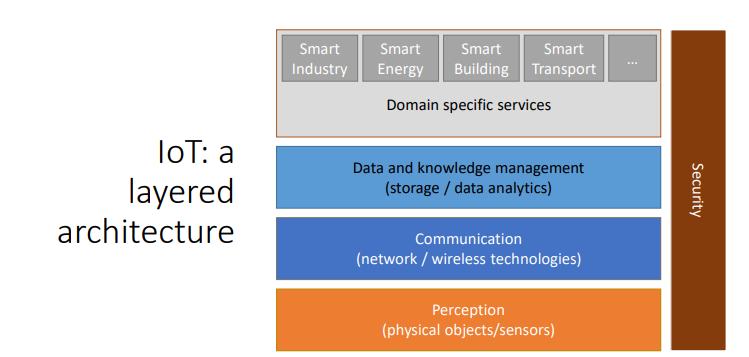
\includegraphics[scale=0.50]{images/Pasted image 20230221153200.png}
	\caption{IoT layered architecture}
	\label{layered-arch}
\end{figure}
And, by istantiating this model we can obtain the following scenario \ref{iot-scenario1}.

\begin{figure}[h]
	\centering
	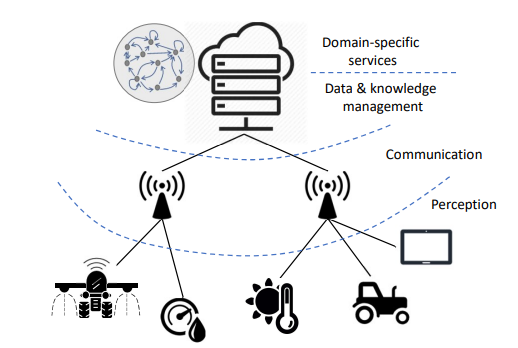
\includegraphics[scale=0.50]{images/Pasted image 20230221153337.png}
	\caption{Simple IoT schema device}
	\label{iot-scenario1}
\end{figure}

\textbf{Sensors} at \textbf{perception layer} can be  of different type based on the nature of activity that need to be carried out:
\begin{itemize}
	\item 
	Specific: they're a fully-functional component and not need to be istantiate along other components to accomplish the desiderated task
	\item 
	Aspecific: they're part of a chain of interaction with other component and this interaction (\textit{e.g. Camera that effect facial recognition task}) allows to perform the intended task
\end{itemize}
\paragraph{Platforms for IoT}\label{sec:platforms-for-iot}
Sensors and actuators are the edge of the cloud: behind internet, data is stored, processed and presented in the cloud. So \textbf{IoT Platforms} provide software layer between IoT devices and applications. Their functionalities may be distributed between devices themself, gateways and server in the cloud or at the edge.
Those platform not allow only data collection but can perform several complex functionalities with a various range of activities (\textit{as mentioned, facial recognition can be a service offered/performed via AWS SageMaker connected to AWS IoT}).
Those platforms allows a wide range of functionalities:
\begin{itemize}
	\item 
	\textbf{Identification}: provides a unique way to identify things in the platform. There are several established standard, based on a given context:
	\begin{itemize}
		\item 
		\textit{IP Address}: for Internet
		\item 
		\textit{MSISDN – Mobile Station International Subscriber Directory Number}: for telephony identification
		\item 
		\textit{URI - Universal Resource Identifier}: on resources exposed to web
		\item 
		\textit{UUID - Universally Unique Identifier}: in computer system and bluetooth-based communication system
	\end{itemize}
	\item 
	\textbf{Discovery}:A mean to find devices, resource and/or services within an IoT deployment inside the same network of devices. This allows also to obtain properties, features and services and locate via identification.

	\item 
	\textbf{Device Management}: as \textit{initial setting} allows to pair, secure setting and key distribution, manage configuration and binding of devices with services, calibrate the sensors, localize devices etc. Managing involves also \textbf{Automatic Software Updates} (\textit{both for software and firmware}), \textbf{device real-time monitoring} (\textit{battery level, internal tempeture, energy consumption}), \textbf{diagnostic/default detection}, \textbf{remote control of devices} (\textit{by activate pheriperals and remote rebooting, without human interaction}) and \textbf{system logging and audit management}.
	Clearly there are different standard based on a given context. The most popular are:
	\begin{itemize}
		\item 
		\textbf{OMA DM (Open Mobile Alliance Device Management)}: mainly for management activity of mobile terminals
		\item 
		\textbf{OMA LWM2M (Open Mobile Alliance Lightweight Machine2Machine}: used for management of IoT devices
		\item 
		\textbf{BBF (Broadband Forum) TR-069}: management for end-users appliances (\textit{e.g. DSL terminals, etc.})
	\end{itemize}
	\item 
	\textbf{Abstraction/Virtualization}: an IoT device is seen as a service so the physical device is associated with its \textit{digital twin}. This provide a way to represent IoT devices and their context, enabling a broad of function on the virtual-device like reasoning and AI-processing over data.
	\item 
	\textbf{Service Composition}: build a composite service by integrating services of different IoT devices and SW components as sketched in \ref{composite-integration}
	\begin{figure}[h]
		\centering
		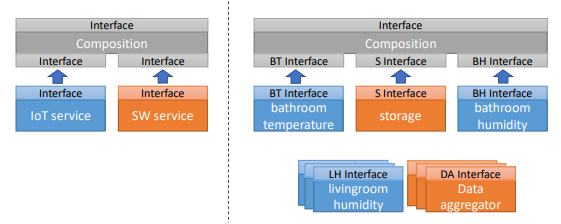
\includegraphics[scale=0.70]{images/Pasted image 20230221155324.png}
		\caption{Example of different service composition}
		\label{composite-integration}
	\end{figure}
	
\end{itemize}

Based on the previous layered architecture model, we add the details just mentioned and provide a general picture on how those are distributed among the layers, obtaining the model pictured in \ref{general-iot-platform}
\begin{figure}[h]
	\centering
	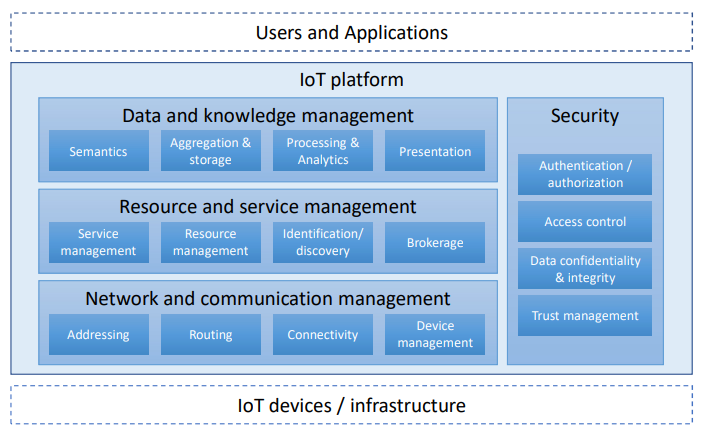
\includegraphics[scale=0.50]{images/Pasted image 20230221155442.png}
	\caption{General layered model for IoT devices}
	\label{general-iot-platform}
\end{figure}

\subsubsection{NoSQL databases}\label{sec:nosql-databases}
No-SQL databases are used in big data and real-time application: they're suitable to scale on horizontal cluster of machines.

As main example, we use \textbf{MongoDB}: what in SQL were \textit{Records} in MongoDB are \textbf{documents}. Documents have a \textit{JSON}-like data syntax: in the following snippet, they're all \textit{field:value} entry.
% json null
\begin{verbatim}
	{ 
		name: "sue", 
		age: 26, 
		status: "X"; 
		group: ["news", "sport"] 
	}
\end{verbatim}

A set of \textit{name/value} pairs are separated by commas: a \texttt{value} can also be an array.
So MongoDB \textbf{documents} correspond to \textbf{native data types} in many programming languages: can embed other documents and arrays to reduce the need for expensive joins.

What were \textbf{tables} in SQL, in \textit{MongoDB} are \textbf{collections}: documents can be grouped in collection but, differently from SQL, different documents in the same collection can have different structure.
\paragraph{Queries}\label{sec:queries}
Usually a \textbf{query} targets a specific \textbf{collection}: it specify criteria and conditions that identify a set of documents in the collection. As SQL, a query can also include a \textit{projection} that specifies the fields to return or include modifier of the output (\textit{like sorting of result, manipulating data format, etc}).  Here an example:
% json null
\begin{verbatim}
	db.sensedData.find({time:{$gt: 1900}}).sort({time:1})
\end{verbatim}

which is represented by the image pictured in \ref{query-example}.
\begin{figure}[h]
	\centering
	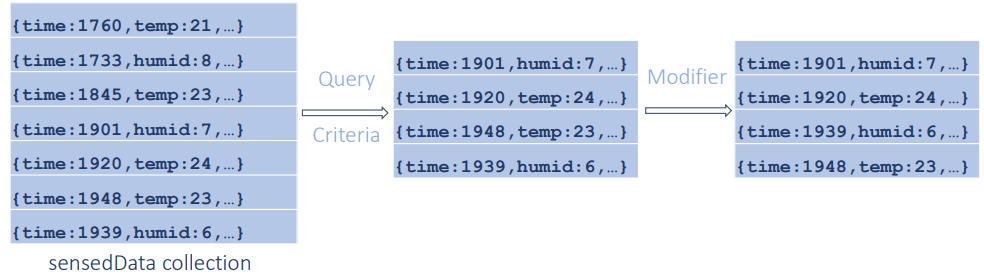
\includegraphics[scale=0.50]{images/Pasted image 20230221160450.png}
	\caption{\texttt{sensedData} query perform}
	\label{query-example}\end{figure}


We can \textbf{modify the data} by update/create/delete: the \texttt{update} and \texttt{delete} operations can specify the criteria to select the documents to update or remove. Here an example of \texttt{insert} query (\textit{referring the pictured in \ref{query-example2}}):
% json null
\begin{verbatim}
	db.sensedData.insert( 
	{ 
		time:2011, 
		humid: 5, 
		... } 
	
	)
\end{verbatim}

\begin{figure}[h]
	\centering
	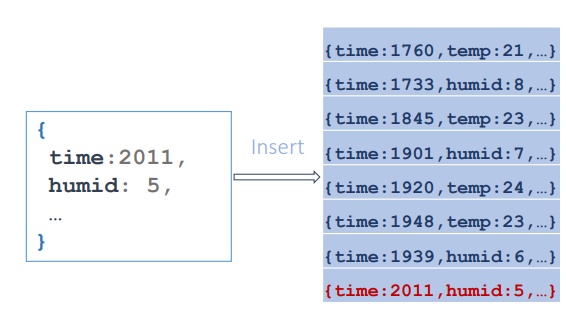
\includegraphics[scale=0.50]{images/Pasted image 20230221160655.png}
	\caption{\texttt{insert} query execution}\label{query-example2}\end{figure}




\subsection{IoT issues}
There are many issues in IoT and they're not easy to address:
\begin{itemize}
	\item 
	\textbf{Performance}: because microcontroller have a very low computation capacity there are physical and computational constraints to evaluate based on the type of activity to perform. This induces to optimize various parameters and metrics.
	\item 
	\textbf{Energy efficiency}: each features it's based on a component that require a minimum level of power to work properly. The \textit{features level} of a device can be tuned, as we will see when discussing about \textbf{duty cycle} \ref{sec:duty-cycle-modulation}. 
	\item 
	\textbf{Security}
	\item 
	\textbf{Data analysis/processing}: how perform analysis and processing in a constrained device or orchestrating the load between several devices in the same network, balancing the overhead between differences neighbors devices.
	\item 
	\textbf{Communication/brokerage/binding}: How to bring together data producers (\textit{sensors}) with consumers (\textit{users/actuators/applications}).
	\item 
	\textbf{Data representation}: data formats and standardization to simplify the multi-vendor device communication.
	\item 
	\textbf{Interoperability}: many standard already exists at different level, like:
	\begin{itemize}
		\item 
		\textbf{MAC Level}: \textit{Bluetooth, IEEE 802.15.4}
		\item 
		\textbf{Network level}: \textit{ZigBee, Bluetooth, 6LowPan,}
		\item 
		\textbf{Application level}: : \textit{MQTT, CoAP, oneM2M}
	\end{itemize}
\end{itemize}


Let's discuss the issues related to \textbf{latency} and \textbf{reliability}, proposing some solutions: this issues arises because the physical devices can be (and they are) far from each other, this without any doubt adds latency to the IoT network. With reliability we mean the process of the network to lose nodes or packets due to some type of \textbf{failure/incident}. We saw 2 approaches:
\begin{itemize}
	\item \textbf{Everything is on the Cloud:} this means that all the processing is done in the cloud, the devices at the perception level are meant only to acquire data and send it to the cloud servers, where all the processing is done. Here latency impacts a lot, since the amount of data sent to the cloud can be significant in term of needed bandwidth.
		\begin{figure}[h]
		\centering
		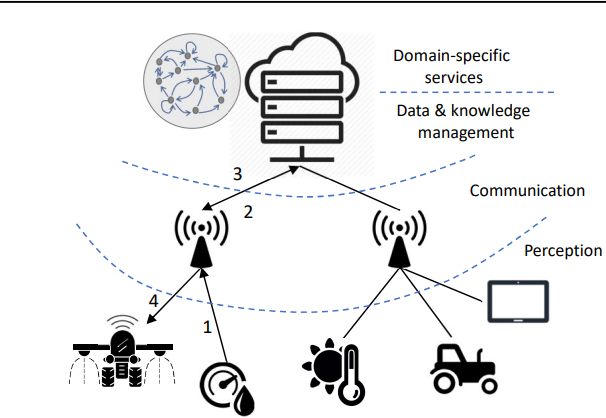
\includegraphics[scale=0.50]{images/Pasted image 20230222185737.png}
		\caption{First approach: everythign on the cloud}
	\end{figure}
			
	
	
	\item \textbf{Some Processing on the Edge}:
	We can adopt some \textit{perception devices (still sensors)} with a little bit of computational power (\textit{small, cheaper cpu}) to process some of the input data, in this way we can reduce the amount of packets sent to the Cloud servers. It's not mandatory to use the cloud, if your devices can make all the processing alone, then you don't need any cloud.
	\begin{figure}[h]
		\centering
		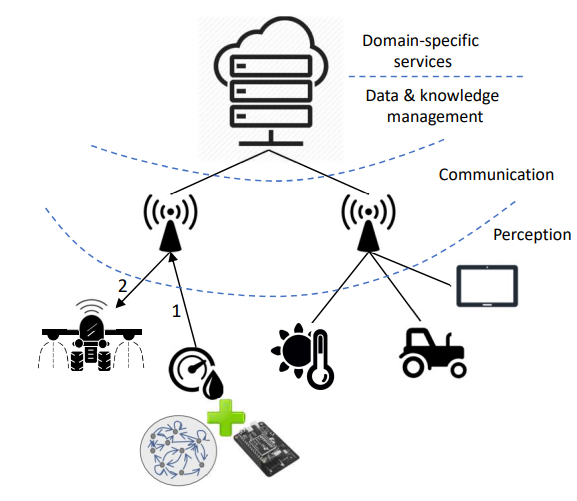
\includegraphics[scale=0.50]{images/Pasted image 20230222185842.png}
		\caption{Second approach: processing on the edge}
	\end{figure}
\end{itemize}


Based on the type of devices, scenario, services offered and computational powered provided closer or farest from the data generation point, we can identify three different \textit{computational models} to apply in an IoT context, as pictured in \ref{scenario1}.

\begin{figure}[h!]
	\centering
	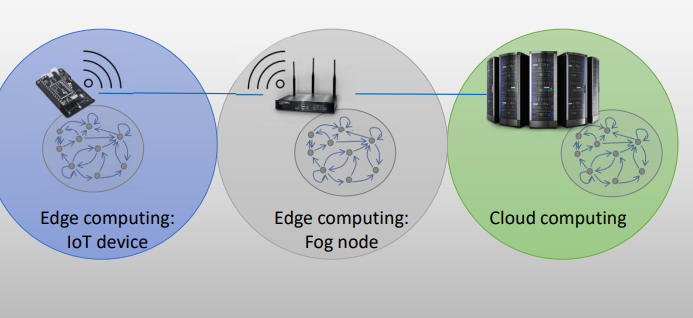
\includegraphics[scale=0.40]{images/Pasted image 20230222191530.png}
	\caption{Three approaches to IoT computational load}
	\label{scenario1}
\end{figure}

\begin{enumerate}
	
	\item \textbf{Edge}: the edge of a typical enterprise network is a network of IoT-enabled devices consisting of sensors and perhaps actuators, these devices may comunicate with one another. A cluseter of sensors can comunicate with a central device that aggregate the data to be collected by a higher level entity. A \textbf{gateway} interconnects the Iot devices with the higher level comunication networks, it performs the traslation between the protocols used in the comunication networks (on top of \textbf{perception} layer) and those used by devices.
	Perception layer uses some protocol that needs to be translated to enter the network. In \textit{a few words}, in the edge we find the \textbf{physical} devices of the perception layer.
	
	
	
	\item \textbf{Fog}: It's an infrastructure of local servers and access points, connected together to provide fast response time to the  \textbf{edge} \textbf{devices} and to reduce the amount of data that goes to the cloud, typically the fog devices are deployed \textbf{physically near the edge}. So rather than storing data \textbf{permanently} or for \textbf{long period} in a central storage we do as much processing as possibile on the \textbf{Fog} level. Processing elements at these levels may deal with high volumes of data and perform data transformation operations, resulting in the storage of much lower volumes of data.\\
	You can think of Fog as the opposite of Cloud, because Cloud \textbf{centralizes storage and processing for a relatively small number of users} while the Fog approach \textbf{distributes processing and storage resources close to the massive number of IoT devices}.\\
	\item \textbf{Core}: the core \textbf{network connects far fog networks and provides access to other networks.} The core network uses high-performance routers, high-capacity transmission lines and multiple interconnected routers for redundancy and capacity. It may connect to other type of devices, such as high performance servers and databases or private cloud capabilities. \textbf{This means that you can connect fog networks to the cloud.}
	
\end{enumerate}



\subsection{AI approach to IoT}\label{sec:the-ai-approach-to-iot}
AI aims at getting computers to behave in a smarter manner, \textbf{either through curated knowledge or through machine learning}.

\begin{figure}[h]
	\centering
	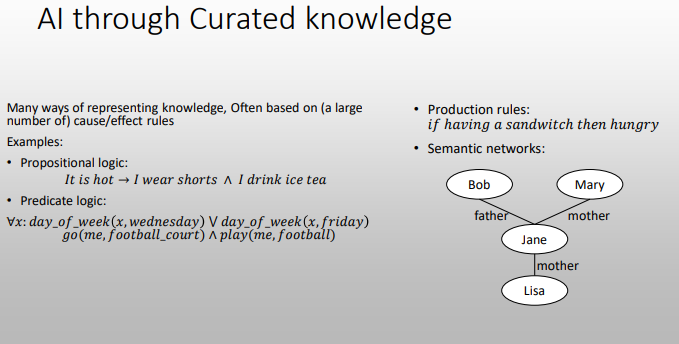
\includegraphics[scale=0.60]{images/Pasted image 20230222192441.png}
	\caption{Curated Knowledge paradigm}
\end{figure}


With \textbf{Machine learning} we indicates a subfield of AI that deals with automatic systems that can learn from data. The system is fed by examples to learn to associate input with output, then when an input (\textbf{never seen}) is given, the model/system produces anyway an output. If \textbf{well trained} the output will mostly be correct, due to generalization capability of ML.\\
Mostly three ML paradigms are used today: the first is the \textit{Unsupervised Learrning} in which the algorithm is presented with a dataset and must find structure or relationships within that dataset on its own. The goal is to identify underlying patterns or groupings within the data. \textit{without any type of labeled data}.\\
The following 2 approaches are the most used in IoT:
\begin{itemize}
	\item 
	\textbf{Supervised learning}:  learn from past examples, \textbf{every example is a pair input + desired output}, aims at predicting the future or interpret the present.
	\item 
	\textbf{Reinforcement learning}: learn from examples, \textbf{but the main difference is that the example is a pair input + reward}, in this way the system knows that the answer is correct if there's a reward. (\textit{E.g. to learn a game the reward can be +1 for winning, -1 for losing, 0 otherwise}).
\end{itemize}

\subsubsection{IoT and emerging Paradigms}\label{sec:iot-and-emerging-paradigms}
\textbf{Blockchain} is a \textbf{shared and trusted public ledger} for making transactions, everyone can inspect and nobody can alter it. the blockchain thus provides a single point of truth: it is shared and \textbf{tamper-evident}, in case of tampering it's quickly noticed.\\
Blockchains shifts the IoT paradigm from \textbf{centralized storage} to a \textbf{decentralized one} in a distribuited ledger. Supports the expanding of the Iot Ecosystem. Since the \textbf{ledger is public} this implies a \textbf{reduce in maintenance costs} and provides trust in data produced. An implementation of this approach can be seen on having different companies that work in a supply chain, everyone of them needs to \textbf{check the quality of the product} along the chain. Each company in supply chain can \textbf{query the ledger} and check the latest transaction, thanks to \textbf{smart contracts} that are used to certify each intermediate transaction.
\subsection{Interoperability \& Reference Standards}\label{sec:interoperability--reference-standards}
A straight implementation of an IoT solution is not a problem by itself, you can design the solution from the bottom (\textit{physical layer}) up to the application layer. This approach is called \textbf{Vertical Silos} (\textit{as there is no external comunication, so even the infrastructure itself is inside the \textit{silos}}) since this system only has your devices and every change/update requires \textbf{your intervention}. This creates a \textbf{Vendor Lock-in} for your clients because the silos prevents them to use devices from other vendors. Vendor lock-in forces high costs to \textbf{migrate} to another vendor, customer need to fully redesign and deploy a new solution.\\
\textbf{Standards} are useful to fix this problem. The first standards we saw are for \textbf{Wireless technologies}:
\begin{figure}[h]
	\centering
	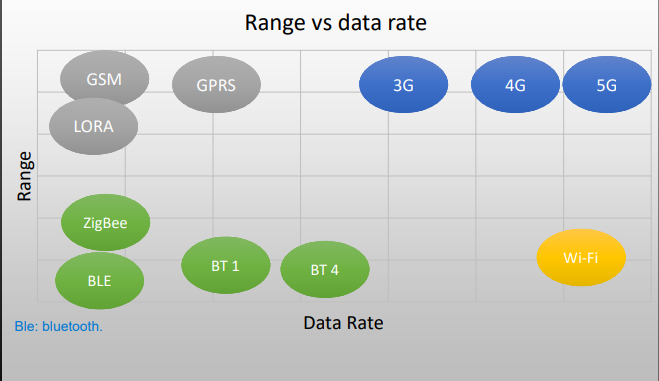
\includegraphics[scale=0.50]{images/Pasted image 20230223102134.png}
	\caption{Standard comparison for range and data rate performances}
\end{figure}


\begin{enumerate}
	\item \textbf{IEEE 802.11} aka \textbf{WIFI}: is a \textbf{family of standards} useful for networks where devices are close to each other (\textit{Range = 100 meters}) but need high data rate. There's a new standard IEEE 802.11A, B, AC. They added new features such as additional frequency bands (5GHz). Since Wi-Fi networks operate on specific frequency bands, with this band the network is faster and less congested. Allows to \textbf{Increase trasmission range and bit rate.} Another useful feature is Roaming between access points, this means that a device changes to the nearest access point in the network.

	
	\item \textbf{IEEE 802.15.4 and Zigbee}: is a wireless communication standard for low-rate wireless networks, where devices are very close to each other (low range). It defines \textbf{both physical and MAC layers}. Usually used when developing low-power sensor networks. The \textit{Low power} property involves also having a \textbf{low throughput} (\textit{115 Kbps, at most}) and low duty cycle (\textit{percentage of time sensor is sensig, as we will see}). Thanks to the fact that Zigbee network can create a \textbf{mesh topology}, we can create larger range networks. In partial mesh topology, nodes basically forward the data to the desired node, in this way the network can grow. The general idea is pictured in \ref{mesh-vs-full}.
	\begin{figure}[h]
		\centering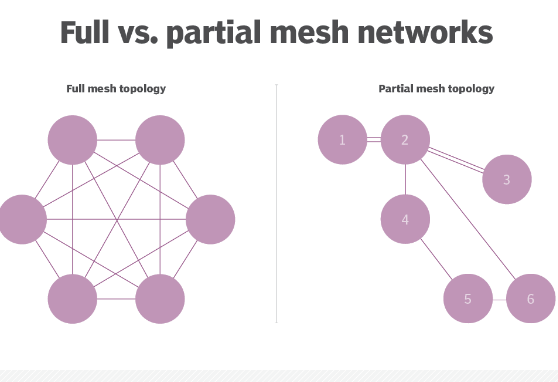
\includegraphics[scale=0.50]{images/Pasted image 20230223100530.png}
		\caption{Full mesh network vs partial mesh network}\label{mesh-vs-full}\end{figure}
	
	
	\item \textbf{Bluetooth}: Higher data rate than ZigBee, but the range is basically the same. Used to make multimedia comunication. Small networks with \textbf{master-slave comiunication}, master sends the data and the slave acquire it.
	
	
\end{enumerate}

\textbf{Why standards?}
Usually motivated by a reduction of the costs for development of a technology, the price for a new technology is high but as soon as other companies try to create the same one this will \textbf{instantly drop the price}. For instance think about a technology that has been developed on the lower layers, in this case comunication layer (Wifi) the companies can move to higher layers in order to create their own technology and sell it at their price.\\
\textbf{Coopetition} stand for \textit{competition and cooperation} so can be a good approach for companies, they work with each other to develop a standard but still deploy their own technologies, built on top of those standards. As said before, this happened for wireless comunications, we saw lot of different standards. \textbf{Interoperability problems moved to the higher layers}.\\
The problem of \textbf{interoperability} arises between consortium of standards.  Nowadays, the problem of interoperability and thus of standarization is moving up at middleware/application layer.
For ZigBee, it covers many layers: it defines a network, transport and application layer specific for ZigBee and incompatible with others.\\
When there are too may standard available and they are not compatible, the solution is to use the concepts of \textit{endpoints} or \textbf{integration gateways}: allows to translate from a given standard to another. The gateway is limited to a single layer but they're able to translate a layer protocol to another one.\\
We have different scenarios/configurations as sketched in \ref{two-type-conf}
\begin{figure}[h]
	\centering
	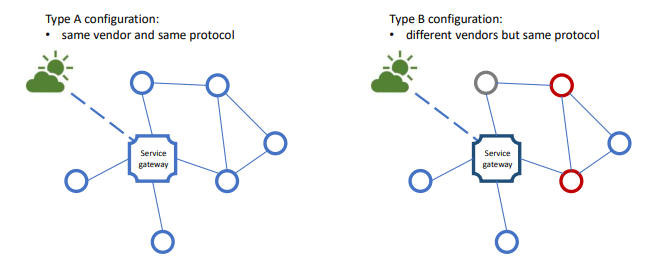
\includegraphics[scale=0.70]{images/Pasted image 20230228112347.png}
	\caption{Service layer within the same standard vs Integration layer for interoperability}
	\label{two-type-conf}\end{figure}

In the left case, even if the same vendor with same protocol, the nodes need a communication to the service gateway that provides access to the internet.
In the right case, we have different vendors that commonly use the same protocol, respecting a common standard: even in this case we need the service gateway to access the rest of the world. The service gateway allows to map \textit{the rest of the world} to interact with it.\\
For devices that are not using internet, there is no need to provide external connectivty: differently for ZigBee or MQTT in which the service gateway provide the functionality of transmitting external data.
Different scenario is pictued in \ref{etherogeneous-conf}: in the left scenario, we have 3 networks which talks using a common standard provided by the \textbf{integration gateway}: in each network, the node talk each other using specific protocols, different from network to network.\\
A \textbf{integration gateway} is able to speak different languages/protocols and able to map one protocol in another. The mapping can be complicated becase can define different behaviours of the devices: in case of a protocol that \textit{push data} and other that differently \textit{pop data} are not translable in one another. So the integration gateway need to translate the \textit{behaviour}: it also need to complete the packet structure, frame tramission, etc.
\begin{figure}
	\centering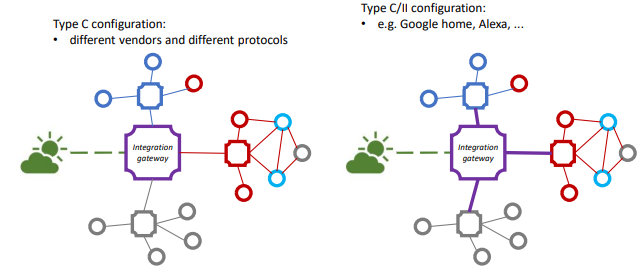
\includegraphics[scale=0.70]{images/Pasted image 20230228112743.png}
	\caption{Integration gateway driven by different vendors and standard consortium}\label{etherogeneous-conf}
\end{figure}
In type C/II scenario (\textit{on the rigth}), the key idea is that the protocol standard or under-the-hood technology is driven by the players (\textit{Google, Amazon}) that in practice determine the specific technology of \textit{integration gateway}, pushing other players to develop in accordance to their technology to guarantee interoperability.

Provide a general purpose integration service is complex: a better solution is forming a \textit{network} of integration gateway that allows to map one protocol to another one or subset of specific-translated protocol. So we obtain a network of \textbf{distributed integration gateways} as sketched in \ref{distribute-gateway}
\begin{figure}[h]
	\centering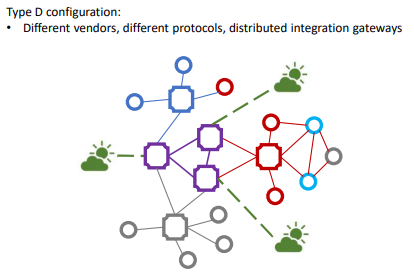
\includegraphics[scale=0.70]{images/Pasted image 20230228114110.png}
	\caption{Distributed integration gateway network}\label{distribute-gateway}\end{figure}

\subsection{Brief Security in IoT}\label{sec:brief-security-in-iot}
There is a crisis point with regard to the security of embedded systems, including IoT devices. The embedded devices are riddled with vulnerabilities and there is no good way to \textit{patch} them. The device manufacturers focus is the functionality of the devices itself so end-users may hve no means of patching the system, having little information about how and when patching.\\
The result is hundreds of millions of internet-connected devices vulnerable to attacks: this lead a problem with sensors that, if attacked, can inject false data into the nework. 
The general context which we refer is pictured in \ref{security-scenario1}
\begin{figure}[h]
	\centering
	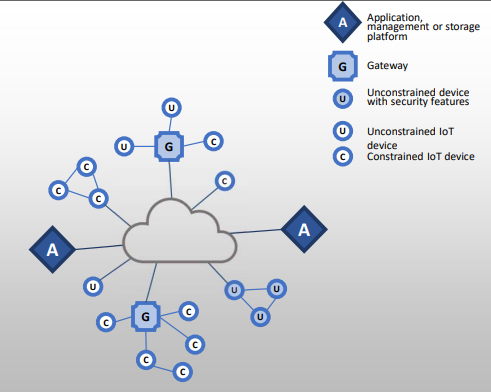
\includegraphics[scale=0.90]{images/Pasted image 20230228114543.png}
	\caption{IoT gateway security: scenario 1}
	\label{security-scenario1}
\end{figure}
Some devices are \textit{constrained, unconstrained} or provide security features: some of them, despite not having security features, they're connected directly with internet.\\
Apply those requirements try to address the problem of security in IoT: the pressure of time-to-market and fasten development phases set the problem of security on devices that are constrained in terms of capabilities or powers so security sometimes became optional because it's not fittable in that types of devices.\\
Usually those devices are not capable to run a full-fledge OS but only a simple OS without security features that are necessary to implement policies, even during updating the software-specific features.\\
The problem arises in the topics of \textit{confidentiality} and \textit{authentication} (\textit{e.g. wearable, physiological sensors}).
\subparagraph{Security Standards}\label{sec:security-standards}
The \textit{IUT-T Standard Recommendation Y.2066} includes a list of \textbf{security requirements} for IoT: those are functional requirements during \textit{capturing, storing, transferring,a ggregating, processing} the data. The requirements concern:
\begin{itemize}
	\item 
	\textbf{Communication security} (\textit{secure, trusted, and privacy protected communication capabilities}): enforces confidentiality and integrity of data during data transmission or transfer
	\item 
	\textbf{Mutual authentication and authorization}: mutual authentication and authorization between devices (or device/user) according to predefined security policies. Before a device (or an IoT user) can access the IoT. The authentication pattern can follow 2 main methods:
	\begin{itemize}
		\item 
		Remote: directly to the cloud but poses complexity due to device's constraints
		\item 
		Local: between devices or authentication service at most one-hop far way or with low overhead for devices
		The mutual authentication is meant as \textit{in both direction between devices and gateway}.
	\end{itemize}
	\item  \textbf{Data management security}: enforces confidentiality and integrity og data when storing or processing data
	
	
	\item \textbf{Service provision security}: deny unauthorized access to service and frauolent service provision. Ensure privacy protection for IoT users.
	
	\item \textbf{Integration of security policies and techniques}: ability to integrate different security policies and techniques. Ensure a consistent security control over the variety of devices and user networks.
	
	
	\item \textbf{Security audit}: any data access or attempt to access IoT applications are required to be fully transparent, traceable and reproducible, according to apporpaite regulations and laws. Support security audit for data transmission, storage, processing and applciation access.
	
\end{itemize}

The \textbf{gateway} is the main building block of the security mechanism and the devices implement only a subset of logic in accordance to the security operations carried out by the gateway.\\
Authentication can happen at different levels: authenticate devices only at physical layer is important but itself it's not a guarantee that the behaviour at the application level is correct (\textit{e.g. tampered device at physical layer}).
There are also other features like protect privacy for devices and gateway, self-diagnosis and self-repair.
A critical phase is the deployment of the devices because initially they're not fully configured and may have not been still identified the correct gateway to connect.\\
An \textbf{IoT gateway} allows the identification of each access to the connected device: the authentication is performed based on application requirements and device capabilities so can either be \textit{mutual} or \textit{one-way}. The first type is more robust than the second one. The \textit{mutual authentication} can also be perfomed between applications.\\
The \textit{security of the data} is based on different security level, defined by the data storage location:
\begin{itemize}
	\item data stored in devices and the gateway 
	\item data transferred between the gateway and devices
	\item data transferred between the gateway and applications
\end{itemize}

\begin{figure}[h]
	\centering
	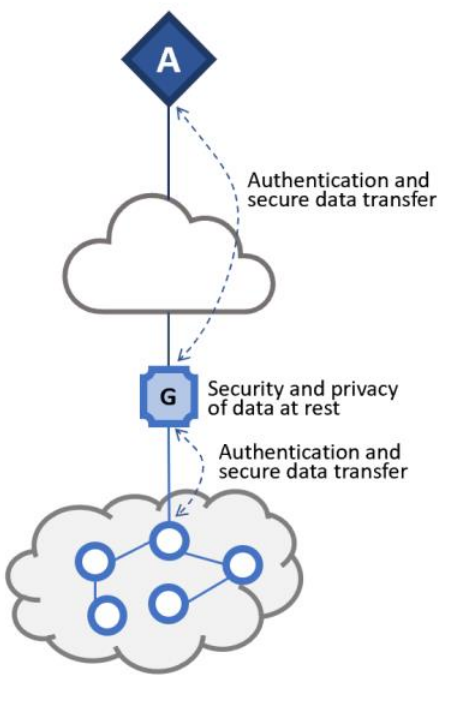
\includegraphics[scale=0.30]{images/Pasted image 20230529150410.png}
	\caption{IoT gateway security - scenario 2}
	\label{security-scenario2}
\end{figure}

These requirements may be difficult to achieve if they involve \textbf{constrained devices}: if the gateway should support security of data stored in devices, without encryption this may be impractical to achieve.\\
These requirements make several refences to \textit{privacy}:
\begin{itemize}
	\item with massive IoT, goverments and enterprises will collect massive amount of data about individuals like \textit{medical information, location, application usage}
	\item privacy is an area of growing concern with the widespread IoT
	
\end{itemize}

\chapter{MQTT - Message Queueing Telemetry Transport}\label{sec:mqtt---message-queueing-telemetry-transport}

\textbf{MQTT} it's  a \textit{lightweight publish/subscribe reliable messaging transport protocol}. It's lightweight thanks to a small code footprint and low network bandwidth, with minimal packet overhead (slightly better than TCP).\\
It's builds upon \textit{TCP/IP} with port \texttt{1883} or \texttt{8883} for using MQTT with SSL (\textit{with overhead}).
MQTT covers application, session and presentation layer (\textit{both directly or undirectly by using middleware}).\\
MQTT uses an instance of \textbf{publish-subscribe} model between users and consumer: internally, as we will see, is implemented as a client-server architecture.
To connect to internet, the IoT devices must adopt internet protocol suite. However, internet stack is too resource-compsuntive respect to constrained IoT devices that usually are \textit{lossy, low power, etc}.\\
Internally MQTT uses a \textbf{client/server} architecture: this bought the major complexities on the server side. It also provide basic \textbf{Quality of Service (QoS)} and it's \textit{data agnostic} so it's suitable both to \textit{M2M (Machine-to-Machine)} and IoT.
\section{Publish/subscribe model}\label{sec:publishsubscribe-model}
The main components of the model are \textbf{publishers, subscribers} and \textbf{broker or event service}. The fist two are both seen as clients and do not know each other, the latter it's the server known both by publishers and consumer.
The \textbf{publisher} produce event or any data: interact only with the \textbf{broker} and does not know if the data is consumed/read by other entities.
The subscribes express interest for an event (\textit{or a pattern of events}): receive the notifications from the broker whenever the event is generated.
Publishers and subscribers never interact each other: they interact indirectly only by the \textit{broker(s)}.
Those pattern allows to be publisher and subscriber to be decoupled in \textbf{time, space and syncrhonization}.

The broker know publisher/subscribers and receive all incoming messages from the first, filter them all and distributed them to the interested subscriber. It also need to manage request of subscription/unsubscription.

A \textbf{publish/subscribe} interaction can be implented in different ways: the boker is usually an \textit{independent} agent and manage, coordinating with publishers/subscribers, the operations of \texttt{publish, subscribe, notify, unsubscribe} as briefly introduced in \ref{mqtt-op}
\begin{figure}[h!]
	\centering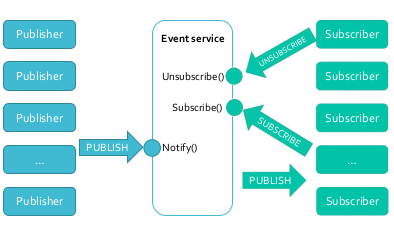
\includegraphics[scale=0.70]{images/Pasted image 20230301091322.png}
	\caption{Operations summary}\label{mqtt-op}
\end{figure}\\
The \textbf{broker} is delegated to storage and management of subscriptions: in figure \ref{mqtt-topic-sub} an example in which different subscribers register themself to one or more \textit{topics} (\textit{smartphone subscribe to \texttt{Temperature \& Humidity} topic} while \textit{computer subscribe only to temperature topic}).
\begin{figure}[h!]
	\centering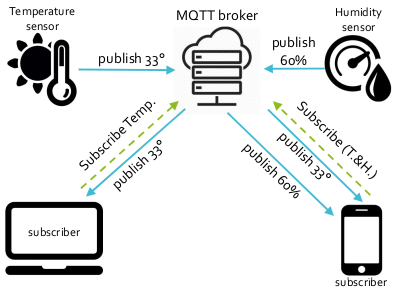
\includegraphics[scale=0.60]{images/Pasted image 20230301091527.png}
	\caption{Example of \texttt{subscribe} for temperature topic}\label{mqtt-topic-sub}
\end{figure}
This model allow to \textbf{decouple the space} because pub/sub do not need to known each other and do not share anything (\textit{they don't known the IP/port of each other and how many peers are subscribed}). It allows also the \textbf{time decoupling} because they don't need to run at the same time, guaranteeing the \textbf{asyncrhonicity} of the model. The asyncrhonous model is pictured in \ref{mqtt-example1}.

\begin{figure}[h]
	\centering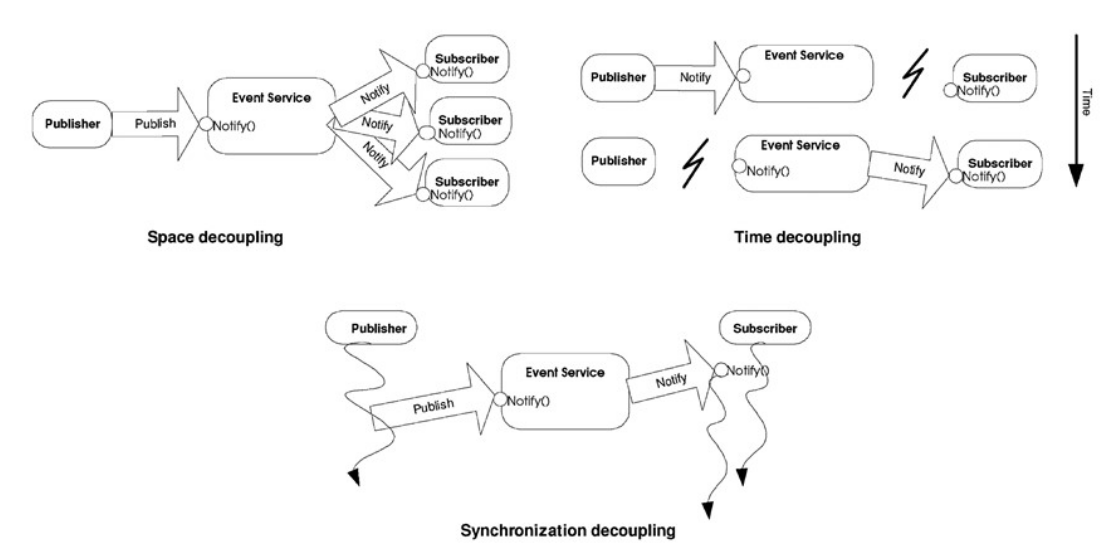
\includegraphics[scale=0.40]{images/Pasted image 20230301091741.png}
	\caption{Asyncrhonous model flow of operations}\label{mqtt-example1}

\end{figure}

The decoupling increments the \textbf{scalability} of the actors involved: the operations on the broker can be easily parallelized and are event-driven, allowing scalability to a very large number of devices by parallelizing the broker.
\subsubsection{Filtering}\label{sec:filtering}
The filtering features managed by the broker can be based on three different criteria:
\begin{itemize}
	\item 
	\textit{Based on \textbf{subject topic}}: the subject (\textit{or topic}) is a part of the message and clients subscribe only to a specific topic. They are usually represented by a string, possible organized in a hierarchical taxonomy.
	\item 
	\textit{Based on \textbf{content}}: the client subscribe for a specific query (\textit{like \texttt{temperature > 30°}}) and that query is used by the broker to filter the messages. This methods involves to understand the semantics of the data transmitted or at least be able to \textit{read} the data so add complexity con context in which security mechanism (\textit{like encryption}) are used to transmit/store data.
	\item 
	\textit{Based on \textbf{type}}: filtering of event is based on both \textit{content} and \textit{structure} so the type refers to the type/class of data that can be customized by the subscriber by defining in a strongly typed language the desired object structure. This methods introduces complexities in case publishers and subscribers are written in different language and there is no a unique \textit{translation of type} because their type system is not uniquely determinate. In those scenarios, tight integration of the middleware and language paradigms (\textit{like Object Programming}) can ease the presented problem.
\end{itemize}
\paragraph{Highlights}\label{sec:highlights}
In the proposed model (\textit{widely sketched in \ref{mqtt-example1}}), publishers and subscriber \textbf{need to agree on topics beforehand} and publisher cannot assume that somebody is listening to the messages because is there are no subscriber messages are not readed by anyone.\\
Despite publisher and subscribers do not need to known each other, they need to known the \textit{hostame/port} of the \textbf{broker} beforehand, to connect and establish a TCP connection to it.
In most application, the delivery of messages is near-real-time but in cases when the subscribers are offline, the broker is able to store the messages \textit{only if} subscribers have been connected with a \textbf{persistent session} and they're already subscribed to the \textit{topic}.  In case of delay or unreliable message the retransmissions is necssary and the latency issues have to been taken into account.
Also the deployment phase take time due to the time needed both by clients to connect to brokers.\\\\
MQTT decouples the syncrhonization allowing to obtain an \textbf{asyncrhonous model}: this model implies the use of callback functions on the subscriber side. Libraries that implements MQTT allows this async model by enabling callbacks.
The complexities of the MQTT protocol are shifted to the \textbf{broker work} which in general represent a much more powerful machine respect to subscribers/clients.

As mentioned, the \textit{subject-based} filtering of a message involves the use of \textit{topic}: topic is based on a hirerarchy of topics that are meaning to the purposes of the appication.
MQTT offers additional \textit{QoS} in term of message reliability: it's based on top of TCP by adding an application level ackwnoledge. It's expressed by 3 levels of QoS (0, 1 ,2) where the last two levels ensure the ACK at application level, while the level $0$ corresponds to TCP reliability level.


\subsection{MQTT operations}

MQTT includes operations at layer 5-6 of ISO/OSI layer, as indicated in \ref{mqtt-iso}.
\begin{figure}[h]
	\centering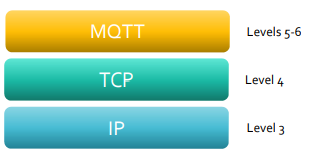
\includegraphics[scale=0.50]{images/Pasted image 20230303163018.png}
	\caption{MQTT in ISO/OSI layer specification}
	\label{mqtt-iso}
\end{figure}
In the following chapter we'll present the main types of messages used in MQTT, how they interact and contribute to the overall protocol flow. 
\subparagraph{CONNECT}\label{sec:connect}
A client connects to a broker by sending a \texttt{CONNECT} message. This enstaurate a \textit{TCP connection} with the broker. The \texttt{CONNECT} message contains:
\begin{itemize}
	\item 
	\textit{Client ID}: it's an optional identifier, if absent is setted to 1.  It's necessary in case of persistent connection: allows to restore connection even in case the connection with the broker is broken, allowing to restore the session from the last \textit{time} the exchange of the message happened. Using no client ID implicit declare the \textit{no session state} so this setting the \textit{Clean Session} flah to true.
	\item 
	\textit{Clean Session (Optional)}: it's FALSE if the client request a persistent session.
	\item 
	\textit{Username/Password (optional)}: No encryption unless used with SSL
	\item 
	\textit{Will flags (optional)}: allows in case of disconnection ungracefully to sent a \textbf{last will message} to the subscribers by the broker (\textit{in case of broken connection with the broker and/or damage}).
	\item 
	\textit{KeepAlive (optional)}: the broker expect to receive from the client periodic message of alive. If not received, the broker can assume that the client is dead and close the TCP connection (\textit{possibly sending the last will message to each subscriber}). The \texttt{KeepAlive = 0} turn of this mechanism, indicating that the subscriber will never send the alive messages to the broker.
\end{itemize}

The broker acknoledges to the CONNECT message with the CONNECTACK message that states if the connection is accepted or rejected and also informs the client (in case of persistent session) information about the previous session.
\subsubsection{PUBLISH}\label{sec:publish}
Each message contains a \textbf{topic} and a \textbf{payload} of whatever type because its managed as a bunch of \textit{bytes}. Only the subscriber is able to understand the semantics of the payload.

The publish message is sent by the publisher to the broker and forgetted. Then it's forwarded by the broker to the subscriber.
The \texttt{PUBLISH} message contains the following data (\textit{summarized in \ref{mqtt-publish}}):
\begin{itemize}
	\item 
	\texttt{packetId}: an integer, is 0 if the QoS level is 0
	\item 
	\texttt{topicName}: string possibly structured in a hierarchy wih slash \textbf{/} delimeters
	\item 
	\texttt{qos}: 0,1 or 2 (\textit{see later})
	\item 
	\texttt{payload}: the actual message in any form (\textit{usually interpreted as bytes})
	\item 
	\texttt{retainFlag}: tell if the message is to be stored by the broker as the last knoen value for the topic. If a subscriber connects later, it will get this message
	\item 
	\texttt{dupFlag}: indicates that the message is duplicate of a previous un-ACKed message. This field is meaningful only if the \texttt{qos} is greather than 0.
	\begin{figure}[h]
		\centering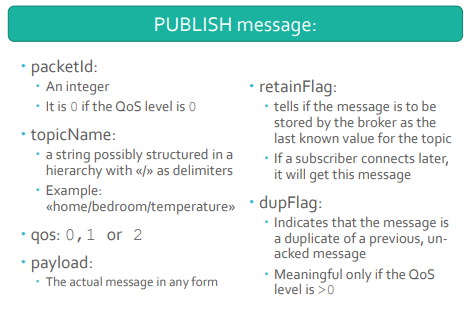
\includegraphics[scale=0.50]{images/Pasted image 20230303165056.png}
		\caption{Publish message structure}\label{mqtt-publish}\end{figure}
	

\end{itemize}
The \texttt{retainFlag} allows to send a specific message for later subscriber, storing it to the broker.\\
When the \textbf{broker} receives a \texttt{PUBLISH} message, it:
\begin{itemize}
	\item 
	acknowledges the message (\textit{if requested, QoS > 0})
	\item 
	processes the message (\textit{identify its subscribers})
	\item 
	delivers the message to its subscribers
\end{itemize}
	The \textbf{publisher}:
\begin{itemize}
	\item 
leaves the message to the broker
\item 
does not know whether there are any subscribers and whether or when they will receive the message
\end{itemize}


\paragraph{SUBSCRIBE}\label{sec:subscribe}
There can be a difference of QoS between \textbf{publisher-broker} and \textbf{subscriber-broker}: even in case of 3 different subscriber with different QoS, the broker will manage them independently.
The structure of the \texttt{SUBSCRIBE} message is the following:
\begin{itemize}
	\item 
	\texttt{packetId}: an integer
	\item 
	\texttt{topic1}: a string (\textit{as in publish message})
	\item 
	\texttt{qos1}: 0,1 or 2
	Usually a \texttt{SUBSCRIBE} message contains a list of \texttt{(topic, qos)} because a subscribe message can refer to multiple topics with the relative QoS.
\end{itemize}

The \textbf{broker} acknowledges the subscriber with a \texttt{SUBACK} message. It contains the following fields:
\begin{itemize}
	\item 
	\texttt{packetId}: the same integer of the relative \texttt{SUBSCRIBE} message
	\item 
	\texttt{returnCode}: one for each topic subscribed. The value \texttt{128} indicates failures (\textit{e.g. the subscriber is not allowed or the topic is malformed}) while \texttt{0,1,2} indicates success with the corresponding QoS granted (\textit{that can be lesser than the QoS requested}).
\end{itemize}
\paragraph{UNSUBSCRIBE}\label{sec:unsubscribe}
A client can unsubscribe a topic to stop receiving the related messages. The \texttt{UNSUBSCRIBE} message is composed by a \texttt{packetId} and a list of topics \texttt{topic1, topic2, ..., topic\_n}. 
The \texttt{UNSUBACK} message have also a \texttt{packetId} and contains the same data of the \texttt{UNSUBSCRIBE} message.

\subsection{Topics}\label{sec:topics}
Topics are strings that are organized into a \textbf{hierarchy} in which each level is separated by a \textbf{/} \textit{slash}.
The subscriber can use \textbf{wildcards} to specify a group of topics:
\begin{itemize}
	\item 
	\texttt{home/firstfloor/+/presence}: select all presence sensors in all rooms of the first floor
	\item 
	\texttt{home/firstfloor/\#}: select all sensors in the first floor
	If using only a dash as a topic, you will subscribe to all topics, including the reserver one.
	Topics that begins with \textbf{"\$"} are reserved for internal statistics of MQTT so they cannot be published by clients. 
\end{itemize}
An HiveMQ example of 5 different topic specification:
\begin{verbatim}
	$SYS/broker/clients/connected 
	$SYS/broker/clients/disconnected 
	$SYS/broker/clients/total 
	$SYS/broker/messages/sent 
	$SYS/broker/uptime
\end{verbatim}

Topics must do not contain space, are short for memory storage optimization and packet size, use ASCII char UTF-8. It's also common practice to embed the clientID in topic or an \textit{unique identifier} like \texttt{sensor1/temperature} so that onlt the client with the same \texttt{clientID} can publish such a topic.
\subsection{Quality of Service}\label{sec:quality-of-service}
The QoS is an agreement between the send and the receiver of a message: the underlying TCP allows the QoS to gurantee delivery and ordering of the messages.
In MQTT the QoS is an agreement between the \textit{clients (publishers/subscribers)} and the \textit{broker}.
MQTT define three levels of QoS:
\begin{itemize}
	\item 
	\textbf{At most once (\texttt{level 0})}: best-effort delivery without guarantees
	\item 
	\textbf{At least once (\texttt{level 1})}: guarantees that a message is delivered at least one time to the receiver
	\item 
	\textbf{Exactly once (\texttt{level 2})}: guarantees that each message is received only once by the intended recipients
	
\end{itemize}
So QoS is used both between publisher and broker and between broker and subscriber.\\
The \textbf{QoS level 0} is called \textit{best effort} delivery because messages are not acknoledge by the receiver. When used between publisher and broker messages are not stored by the broker and immediately forwarded.
It provides the same guarantees as the TCP Protocol by guaranteeing the delivery as long as the connection remains. If one of the two peers disconnect there's not guarantee anymore.\\
Messages are numbered and stored by the broker until they are delivered to all subscribers with \textbf{QoS level 1}. Each message is delivered at least once to the subscribers with QoS 1. A message may be delivered more than once so it's suitable when the subscribers can handle the management of duplicated messages.
Subscribers send acknowledgements by sending \texttt{PUBACK} packets.\\\\
The \textbf{QoS level 2} is the slowest mechanism to guarantee QoS because check that each message is received exactly once by the recipient.\\ 
It uses a \textbf{double two-way handshake} by sending \texttt{PUBLISH} and the relative ACK by the \texttt{PUBREC} Packet. Respectively, the client send \texttt{PUBREL} to acknoledge the reception of the message: the broker now can drop the message from its storage and declare the transmission complete by sending a \texttt{PUBCOMP} packet.\\
So for each message of QoS level 2 there is need four times the exchange of packets required by the level 0.
To summarize QoS level 2, the figure \ref{mqtt-qos-2}, describe the entire exchange.
\begin{figure}[h]
	\centering
	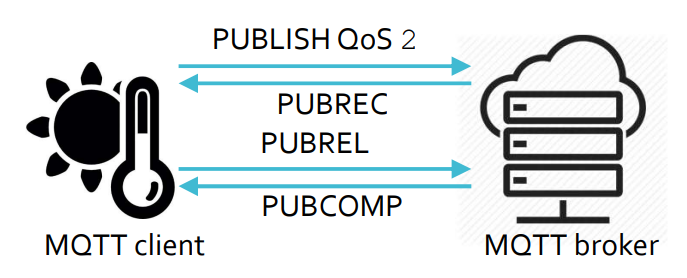
\includegraphics[scale=0.50]{images/Pasted image 20230304093804.png}
	\caption{MQTT QoS $2$ message exchange diagram}\label{mqtt-qos-2}\end{figure}

In \textit{QoS level 2}, the \textbf{broker}:
\begin{enumerate}
	\item 
	receives the PUBLISH with a message
	\item 
	Process the PUBLISH
	\item 
	Sends back a PUBREC
	\item 
	Keeps a reference to the message until it receives PUBREL
\end{enumerate}

The \textbf{client}:
\begin{itemize}
	\item 
Sends PUBLISH with a message
\item 
Waits for PUBREC and then store PUBREC and discards the message
\item 
Sends back a PUBREL to inform the broker
\item 
Waits for PUBCOMP and then discards the PUBREC	
\end{itemize}



The \textit{double two-way handshake} is necessary because the first handshake allows to send the message, the second is to agree to discard the state. The \texttt{PUBREC} message alone is not sufficient because if it's lost, the client will send again the message so the broker needs to keep a reference to the message to identify duplicates. With \texttt{PUBCOMP} the client know that it can discard the state associated to the message.
This level of QoS is suitable when the clients \textit{cannot manage duplicates} so the complexity to guarantee avoiding duplicates is managed by the broker that keep tracks of ACK and stores messages, with high overhead.
\subsection{Persistent sessions}\label{sec:persistent-sessions}
Persistent sessions keep the state between the client and the broker: if a subscriber disconnect, when it connects again, it does not need to subscribe again the topics. The session is associated with the \texttt{clientId} defined with the \texttt{CONNECT} message.
In a persistent session the data stored are:
\begin{itemize}
	\item 
	All subscriptions to topics
	\item 
	All QoS \texttt{1,2} messages that are not confirmed yet
	\item 
	All QoS \texttt{1,2} messages that arrived when the client was offline
\end{itemize}
A persistent session is requested at \texttt{CONNECT} time (\textit{\texttt{cleanSession} flag setted to FALSE}): the \texttt{CONNACK} message confirms whether the session is persistent.\\
Also clients have to \textbf{store state} in persistent session:
\begin{itemize}
	\item 
	Store all messages in QoS \texttt{1,2} flow, not ACKED By the broker
	\item 
	All received QoS \texttt{2} messages not confirmed by the broker
	
\end{itemize}
Messages of persistent sessions will be stored as long as the system allows it. The persistent mechanism can be avoided when refers to publishing-only clients that uses only QoS level 0 or if old messages are not important or when miss some data is not a problematic.

\subsection{Retained messages}\label{sec:retained-messages}
A publisher has to gurantee that its messages are actually delivered to the subscriber, even for later subscriber. When a client connects to the broker and subscrbes a topic, it does not known when it will get any message. For each topic, we can have \textbf{only one retained messages}, generally the \textit{last one message} sent by the publisher. This way a new subscriber is immediately updated with the \textit{state of the current communication}.\\
A retained message is a normal message with the flag \texttt{retainFlag} setted to \texttt{TRUE}: the message is stored by the broker so if a new retained message is published, the broker will keep the last one received.
When a \textit{client} subscribes the topic of the retained message, the broker immediately sends the retained message for that topic: this can also works combined with \textbf{wildcards}.\\
The mechanism of \textbf{retained messages} and \textbf{persistent sessions} are completely decoupled: the second are messages kept by the server even if they had already been delivered. To delete a retained message is sufficient to publish a retained \textbf{empty} message of the same topic. This mechanism is usefull for \textit{unfrequent updates} of a topic: for \textit{example}, consider a device that update its status (\texttt{ON/OFF}) on topic \texttt{home/devices/device1/status} so if it publish ON, this status will remain for long time and if the message if retained, all subscribers will easily know the device is on.
\subsection{Last will and testament}\label{sec:last-will-and-testament}
Last will and testament feature is used to \textbf{notify other clients about the ungraceful disconnection of a client}. At \texttt{CONNECT} time, a client can request the broker a specific behavior about its last will: it's a normal message with \texttt{topic, retainFlag, QoS} and \texttt{payload} stored by the broker as a last will.
When the broker detects the client is \textbf{abruptly disconnected}, it send the last will message to all subscribers of the topic specific in the last will message. If the client send \texttt{DISCONNECT}, the stored last will message is discarded because the underlying assumption is that before correctly disconnect the clients has been already notified other clients.
So, the broker sends a last will message if:
\begin{itemize}
	\item 
	Occurs an IO Network error
	\item 
	The client does not send the \texttt{KeepAlive} message in time
	\item 
	The client closes the network connection without sending \texttt{DISCONNECT}
	\item 
	The broker closes the connection with the client because of a protocol error
\end{itemize}

The last will is specified in the \texttt{CONNECT} Message and contains 4 optional fields:
\begin{itemize}
	\item 
	\texttt{lastWillTopic}: a topic
	\item 
	\texttt{lastWillQoS}: either 0,1,2
	\item 
	\texttt{lastWillMessage}: a string
	\item 
	\texttt{lastWillRetain}: a boolean flag
\end{itemize}

The last will message can be combined with \textbf{retained messages}: imagine a scenario in which a devices updates the status (\texttt{ON/OFF}) on topic \texttt{home/devices/device1/status} so it's powered and publish \texttt{ON} with a \textit{retained message}. If the device crashes and then it abruptly disconnect, it does not publishes \texttt{OFF}: \textit{last wll message} can be useful here because could be a retained message with payload \texttt{OFF} so the \textbf{subscribers and the futures ones are properly informed}, even in case of unwanted disconnection.
\subsection{KeepAlive}\label{sec:keepalive}
The KeepAlive mechanism assure that a client and its connection with the broker is still \textbf{alive}: the client sends periodics messages to the broker that prove its liveness. The \textit{frequency} of these messages is declared in the \texttt{CONNECT} message. The keep alive message must be sent by the client before the connection expiration of the interval set with the CONNECT message. The entire process is sketched in \ref{mqtt-keepalive}
\begin{figure}[h]
	\centering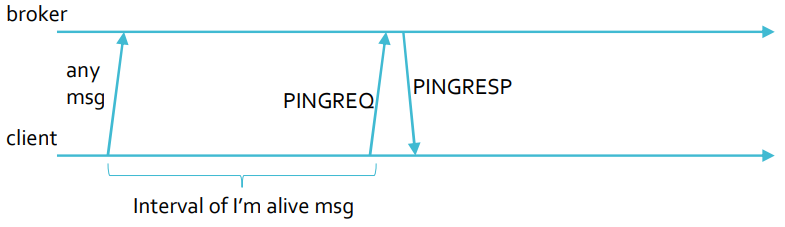
\includegraphics[scale=0.50]{images/Pasted image 20230304101151.png}
	\caption{\textit{KeepAlive} message flow}\label{mqtt-keepalive}
\end{figure}

\textbf{KeepAlive} timer (\textit{managed by the broker to control the liveness}) is resetted by both \texttt{PINGREQ} messages and by pulbish a message on a topic: this allows to be consired alive by the broker. So if the client does not send \texttt{PINGREQ} in time or any other message, the broker turns off the TCP connection and sends the last will message.
\subsection{Packet format}\label{sec:packet-format}
The structure of an MQTT \textbf{control packet} is the following:
\begin{figure}[h!]
	\centering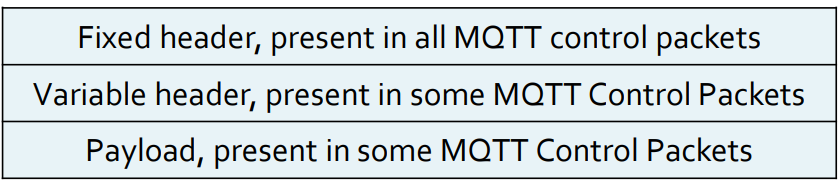
\includegraphics[scale=0.40]{images/Pasted image 20230304101920.png}
	\caption{Control packet structure}
\end{figure}

The \textbf{fixed header} is composed by \textbf{2 bytes}, the first contains (\ref{fixed-header-bytes}):
\begin{figure}[h]
	\centering
	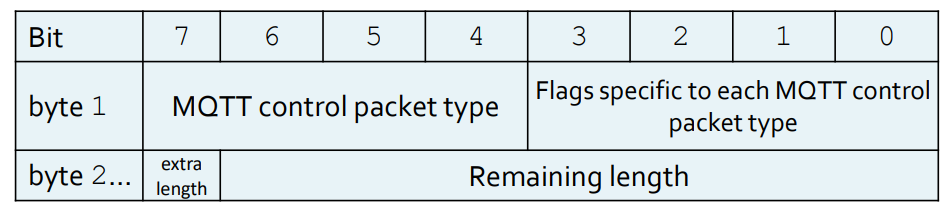
\includegraphics[scale=0.35]{images/Pasted image 20230304101933.png}
	\caption{Fixed header structure}\label{fixed-header-bytes}
\end{figure}

\begin{itemize}
	\item 
	\textit{MQTT Control packet type}: 4 bit (\textit{range 7 to 4})
	\item 
	\textit{Flags specific to each MQTT control packet type}: 4 bit (\textit{range 3 to 0})

\end{itemize}
The second byte contains the \textbf{remaining length} which is the \textbf{length} of the variable header and payload: 7 bits are used to encode the remaining length while one bit (\textit{the MSB, index 7}) is a flag that specifies that there is another field.
The \textbf{control packet type} are pictured in \ref{mqtt-control-packet-type}
\begin{figure}
	\centering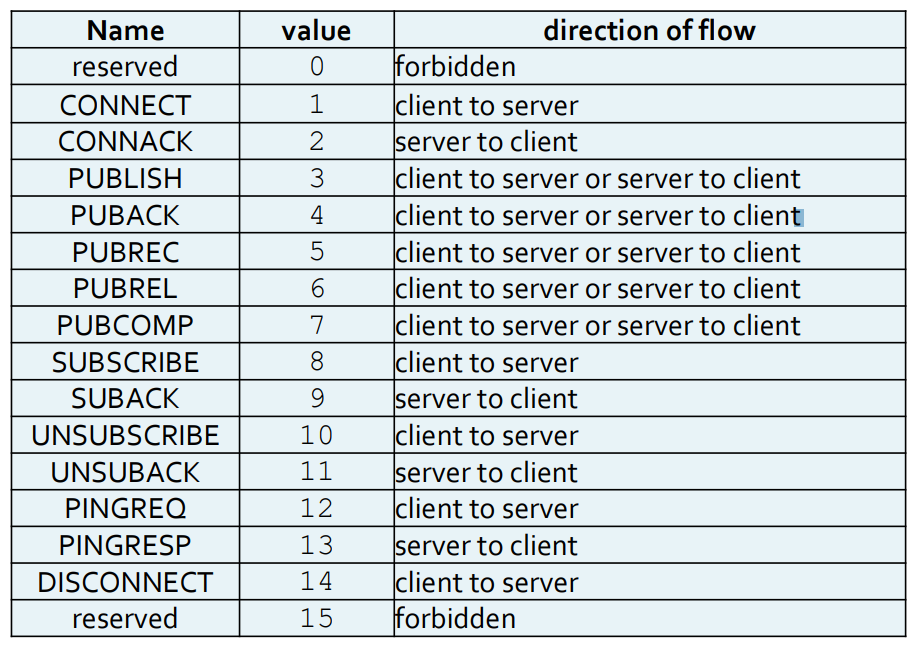
\includegraphics[scale=0.30]{images/Pasted image 20230304102050.png}
	\caption{Control packet type}\label{mqtt-control-packet-type}\end{figure}

The \textbf{variable header} contains the \texttt{packetId} (\textit{encoded with 2 bytes)}, only the packets regarding the \texttt{CONNECT} and \texttt{CONNACK} does not contains the \texttt{packetId} while the \texttt{PUBLISH} packet contains this information only if \texttt{qos > 0}. It can contains other information depending on the control packet type: for example, \texttt{CONNECT} packets include the protocol name and version, plus a number of flags (\textit{see CONNECT)}.\\
The \textbf{payload} can be empty or, in case of \texttt{CONNECT} message it contains data about the client or for \texttt{PUBLISH} can be optional (\textit{empty payload are allowed, e.g. to reset retained message}). For example, the \texttt{CONNECT} packet includes:
\begin{itemize}
	\item 
	client identifier (mandatory)
	\item 
	will topic (optional)
	\item 
	will message (optional)
	\item 
	Username (optional)
	\item 
	Password (optional)
	
	
\end{itemize}
In the table \ref{mqtt-req-data} is listed when the payload is required. 
\begin{figure}[h!]
	\centering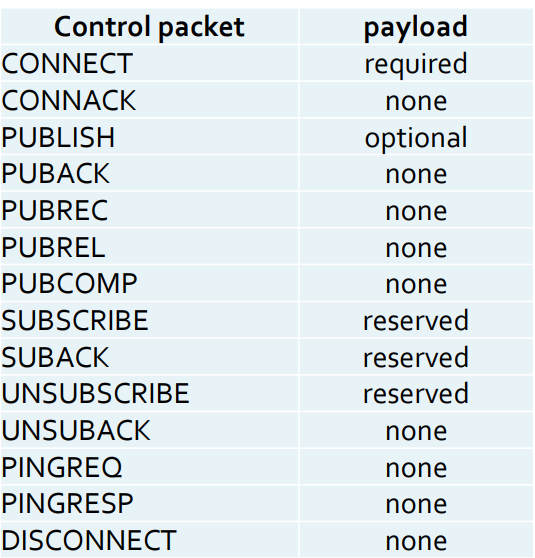
\includegraphics[scale=0.40]{images/Pasted image 20230304102808.png}
	\caption{MQTT required payload commands}\label{mqtt-req-data}\end{figure}


\section{MQTT on Arduino}\label{sec:mqtt-on-arduino}
Include only a subset of MQTT specific, excluding:
\begin{itemize}
	\item 
	SSL/TLS
	\item 
	QS level 2
	\item 
	Payload limited to \texttt{128} bytes
\end{itemize}
\iffalse
\paragraph{Constructors}\label{sec:constructors}\begin{itemize}
	\item 
	\texttt{PubSubClient()}
	\item 
	\texttt{PubSubClient (server, port, [callback], client, [stream])}: create a fully configured client instace. The API includes other \textit{PubSubClient} with lesser parameter. The parameters are:
	\begin{itemize}
		\item 
		Server address: IP address of the broker (\textit{as an \texttt{IPAddress} object})
		\item 
		Port: port used by the broker. Because SSL/TLS is absent, usually is the 1883.
		\item 
		Callback: a pointer to a function that allows to distinguish between subscriber, publisher or both. They are implemented on top of interrupts and allows to intercept publishing/invokation.
		\item 
		Client: an instance of the \texttt{Client} class that cna connect to a specified internet IP address and \texttt{portCLlient} (\textit{e.g \texttt{EthernetClient}})
		\item 
		Stream: an instance of \texttt{Stream}, used to store received messages (\textit{e.g. \texttt{mqtt\_stream}})
	\end{itemize}
\end{itemize}

\paragraph{Functions}\label{sec:functions}\begin{itemize}
	\item 
	\texttt{boolean connect(clientId, username, password, willTopic, willQoS, willRetain, willMessage)}: connect the client, specifyng the \textbf{will message}, username and password (\textit{as basic authentication mechanism})
	\item 
	\texttt{void disconnect}
	\item 
	\texttt{int publish(topic, payload, length, retained)}: publishes a message to the specified topic, with the \textbf{retained flag} as specified. Return \texttt{FALSE} if publish fails, either due to connecion lost or message too long, while return \texttt{TRUE} if publish succeeds. The API includes other \texttt{publish()} with lesser methods.
	\item 
	\texttt{boolean subscribe (topic, [qos])}: topic is a \texttt{const char []}, payload is a \texttt{byte[]}, length is \texttt{byte}, retained is \texttt{boolean} and qos is an \texttt{int}.
	\item 
	\texttt{boolean unsubscribe(topic)}:
	\item 
	\texttt{boolean loop()}: to support the keepAlive features
	\item 
	\texttt{int connected()}: check whether the client is connected to the server
	\item 
	\texttt{int state()}: return the current state of the client
	The following function configure the parameter to the server if still not initialized by the constructor:
	\item 
	\texttt{PubSubClient setServer (server, port)}
	\item 
	\texttt{PubSubClient setCallback (callback)}
	\item 
	\texttt{PubSubClient setClient (client)}
	\item 
	\texttt{PubSubClient setStream (stream)}

\end{itemize}

	See more bootstrap example at \href{https://pubsubclient.knolleary.net/api}{https://pubsubclient.knolleary.net/api}.
\fi
\subsection{MQTT Competitors}\label{sec:mqtt-competitors}
HTTP is a valid alternative to MQTT, despite it's not speficially designed to operate for IoT devices at appliaiton level. A comparison is sketched in \ref{mqtt-vs-http}.
\begin{figure}[h!]
	\centering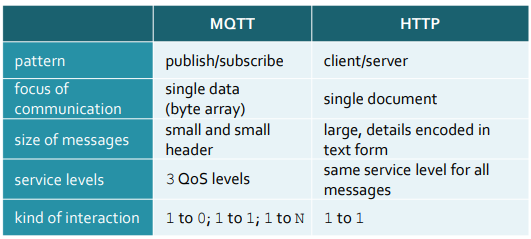
\includegraphics[scale=0.70]{images/Pasted image 20230307112648.png}
	\caption{MQTT vs HTTP}\label{mqtt-vs-http}\end{figure}

HTTP used in IoT device can be used in two different ways:
\begin{enumerate}
	\item 
	Clients are server accept connection from services
	\item 
	Service is the server and accept incoming connection from clients (devices). 	This paradigm poses problems on scalability, also considering the size of messages and the focus of communication (\textit{because HTTP is not suitable for constraned devices}).
	In real world application both solution are deployed (\textit{e.g. TeamSpeak, AWS IoT}) because nowadays devices are not entirely constrained on power/computation capacity.
\end{enumerate}

There are several \textbf{limitations} on MQTT: the need for a centralized broker can be limiting in scenario where we have several point-to-point communication because the overhead of a broker may easily become not compatible with end devices capabilities as the network scales up. Also, the broker is a \textbf{single point of failure} and the underlying TCP protocol does not come for free: it's not cheap for low end devices. Exists also an MQTT based on UDP, not standardized nowadays.
\subsection{Brief CoAP (Constrained Application Protocol)}\label{sec:brief-coap-constrained-application-protocol}
Standardized in \texttt{RFC-7252}, it's specialized for \textbf{web transfer} and it's suitable for machine-to-machine for use with constrained nodes and constrained networks. It used under the hood the UDP Protocol. The general key idea is pictured in \ref{mqtt-vs-coap}
\begin{figure}[h]
	\centering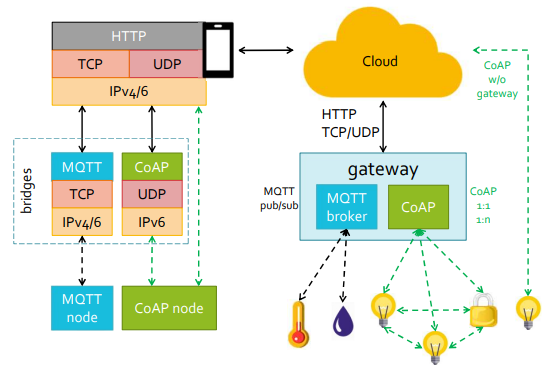
\includegraphics[scale=0.50]{images/Pasted image 20230307113500.png}
	\caption{MQTT vs CoAP}\label{mqtt-vs-coap}\end{figure}


CoAP also support a direct connections between devices, without relying on an intermediate bridges to translate/support the communication.

CoAP is designed to work with nodes with \textit{8 microcontrollers} with small amounts of ROM and RAM.  Constrained networks such as IPv6 over 6LoWPANs: it concerns the size of the header, compressing addresses and header used in IPv6.\\
The main strenghts are that is \textit{native UDP, support multicast, security mechanism are embedded in the RFC itself, suppport asyncrhonous communication by design}. There are also weakes as \textit{standard maturity} and \textit{message reliability not quite sophisticated, similar to MQTT QoS}.



\chapter{ZigBee}\label{sec:zigbee}
\textit{ZigBee} covers almost all layer from \textit{phyisical} to \textit{application} layer: it's a standard protocol for wireless sensors and actuators networks thus is considered an IoT standard even if use TCP/IP as its internal mechanism.
The protocol is developed and promoted by industrial private alliance called ZigBee alliance.\\
It covers different application cases like \textit{home automation, health care, consumer and industrial automation}. It's a competing standard with Bluetooth, especially in eHealth environment where ZigBee failed but had more successfull application in other sectors.

The main requirements that drove the designing of the protocol were:
\begin{itemize}
	\item 
	\textit{Network completely autonomous}: self-organiziting with minimal or nothing manual intervention
	\item 
	\textit{Very long battery life}: ideally a ZigBee device should last 10 years
	\item 
	\textit{Low data rate}: allows to guarantee a very long battery life by optimizing performances. This allows trading performances for battery life.
	\item 
	\textit{Interoperability} of ZigBee devices from different vendors
\end{itemize}

This criteria resulted in some \textbf{main features}, like being \textit{standard based, low cost} and \textit{globally-enabled} by allowing a range of private frequencies based on user parameters (\textit{there are constraints country-specific for frequencies}), \textit{reliable and self-healing}, \textit{large number of node support} by allowing up to $30.000$ devices in a short ranges (\textit{$200$ meters}) and also for larger range by supporting \textit{multi-hop network}. Those combination of charateristics allows an easy deploy and a very long battery, also guarateeing advacend \textit{security mechanism.}\\
Despite is not explicitly mentioned in the specific itself, the \textit{transport layer} features are implemented by some \textbf{sub-layers} between network and MAC layer.
\paragraph{IEEE 801.15.4 Standard}\label{sec:ieee-801154-standard}
Define the specification of the \textbf{physical} and \textbf{MAC layers} for \textit{low rate PAN}. It operates on top of the frequencies of WiFi and Bluetooth: using the same frequencies but not perceived or talk each other, just consider each other as \textit{noise}. The frequency that are defined by the specification are:
\begin{itemize}
	\item 
	$868–868.6 MHz$ (\textit{e.g., Europe}) with a data rate of $20$ kbps
	\item
	$902–928 MHz$ (\textit{e.g., North America}) with a data rate of $40$ kbps
	\item 
	$2400–2483.5 MHz$ (\textit{worldwide}) with a data rate of $250$ kbps
\end{itemize}

\section{ZigBee Standard}\label{sec:zigbee-standard}
The components described in the ZigBee specification are pictured in \ref{zigbee-specification}. 
\begin{figure}[h!]
	\centering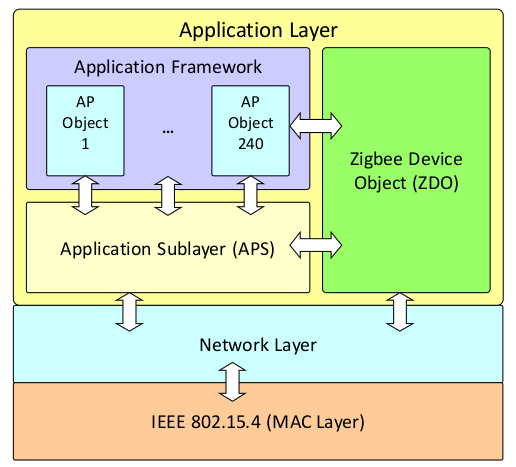
\includegraphics[scale=0.40]{images/Pasted image 20230307162949.png}
	\caption{ZigBee Specification overview}
	\label{zigbee-specification}
\end{figure}

The Application layer of ZigBee is defined by 3 sub-layer:
\begin{enumerate}
	\item 
	\textbf{Application Framework}: contains up to $240$ \textbf{\textit{Application Objects (APO)}} in which each APO is a \textit{user-defined ZigBee application}.
	\item 
	\textbf{ZigBee Device Object (ZDO)}: provides services to let the APOs organize into a distributed application. Guarantee interoperability between different devices of different vendors
	\item 
	\textbf{Application Support sublayer (APS)}: provides data and management services to the APOs and ZDO.
\end{enumerate}
The workflow of those three sublayers will be addressed in detail in \ref{sec:application-layer}.
\subsection{Service primitives}\label{sec:service-primitives}
Each layer provides its data and magement service to the upper layer so \textbf{each service} is specified by a set of primitives of four generic types.
Between all the services and all the layer, only \textbf{4 primitives} are used/consumed between each layer as sketched in \ref{4-primitives-layer}:
\begin{itemize}
	\item 
	\textbf{Request}: It is invoked by the upper layer to request for a specific service;
	\item 
	\textbf{Indication}: It is generated by the lower layer and is directed to the upper layer to notify the occurrence of an event related to a specific service;
	\item 
	\textbf{Response}: It is invoked by the upper layer to complete a procedure previously initiated by an indication primitive;
	\item 
	\textbf{Confirm}: It is generated by the lower layer and is directed to the upper layer to convey the results of one or more associated previous service requests.
	Services may not use all the four primitive (\textit{see later}).

\end{itemize}
	\begin{figure}[h]
	\centering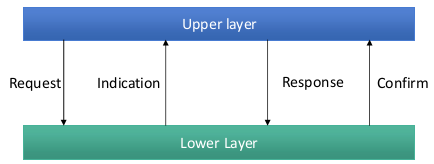
\includegraphics[scale=0.50]{images/Pasted image 20230307163527.png}
	\caption{Layer interaction}
	\label{4-primitives-layer}
\end{figure}

In figure \ref{zigbee-com-example} an example of \textit{service primitives} that allows to visualize the flow: same levels of different nodes interact by means of those 4 primitives.
\begin{figure}[h]
	\centering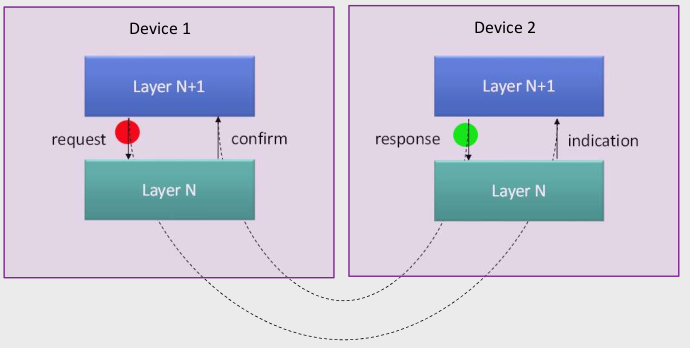
\includegraphics[scale=0.40]{images/Pasted image 20230307163642.png}
	\caption{Communication between two devices, using basic primitives}
\label{zigbee-com-example}
\end{figure}

\paragraph{Data transfer}\label{sec:data-trasnfer}
The data transfer between node assume an uniform name called \textbf{Data Unit}, encapsulated at different level with different packet layers, here specified in \ref{data-unit-layer}.

\begin{figure}[h]
	\centering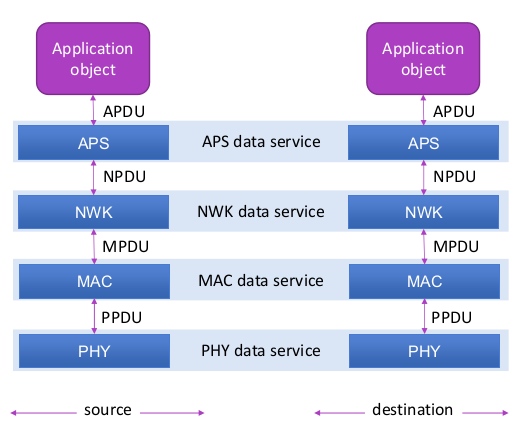
\includegraphics[scale=0.40]{images/Pasted image 20230307163743.png}
	\caption{Data Unit per layer}
	\label{data-unit-layer}
\end{figure}
For each layer the \textit{data unit} are specific:
\begin{itemize}
	\item 
	\textit{Application Protocol Data Unit}
	\item 
	\textit{Network Protocol Data Unit}
	\item 
	MAC Protocol Data Unit
	\item 
	\textit{Physical Protocol Data Unit}
\end{itemize}
\subsection{Network Layer}\label{sec:network-layer}
At network level we identify 3 types of devices:
\begin{enumerate}
	\item 
	\textbf{Network coordinator}: Despite been a infrastructurless protocol, a coordinator have the function of create the network by taking decisions/interfacing with the rest of the network. Allows to bootstrap the network.
	\item 
	\textbf{Router}: provide routing features in a large network and can also have services capability. From the point of view of routing capabilities, they have the same capabilities of a coordinator.
	\item 
	\textbf{End device}: they are not able to communicate alone with the rest of the network and use coordinators/routers to communicate. They must be attach to the coordinator to be able to communcate over the network. They do not need to implement the entire standard, differently from router/coordinators that must have the capabilities to implement the standard fully. Generally they correspond to a RFD \textit{Reduced Functional Interface} while routers/coordinator are FFD \textit{Full Functional Device}.
	
\end{enumerate}
We can have different \textbf{network topologies} as shown in \ref{net-topologies}.
In a \textbf{star shaped topology}, the router have the same roles as end device: they uses the \textit{superframe}. In the \textbf{tree topology}, the \textit{multi-hop network} (\textit{not fully addressed in those notes}) functionalities are supported and the nodes can communicate only via the intermediary routers: they can or cannot use \textit{superframes}. In \textbf{mesh networks}, the communication is possible even between nodes witout relying on the \textit{superframe infrastructure} (\textit{superframe is the topic of the lecture on CSMA/CA, see later chapters}).

\begin{figure}[h]
	\centering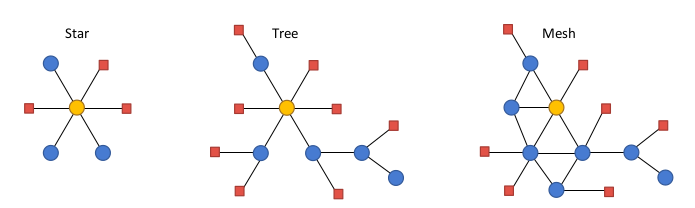
\includegraphics[scale=0.50]{images/Pasted image 20230307164039.png}
	\caption{ZigBee supported network topologies}
	\label{net-topologies}
\end{figure}


The \textbf{network layer} provides services for:
\begin{enumerate}
	\item 
	Data transmission (\textit{both unicast \& multicast})
	\item 
	Network initialization
	\item 
	Devices addressing
	\item 
	Routes management \& routing
	\item 
	\textit{Management of joins/leaves of devices}: because the networks is formed incrementally, formed a network with an arbitrary topology.
\end{enumerate}

The \ref{table-primitives} table summarizes which services uses the 4 primitives already mentioned:

\begin{figure}[h!]
	\centering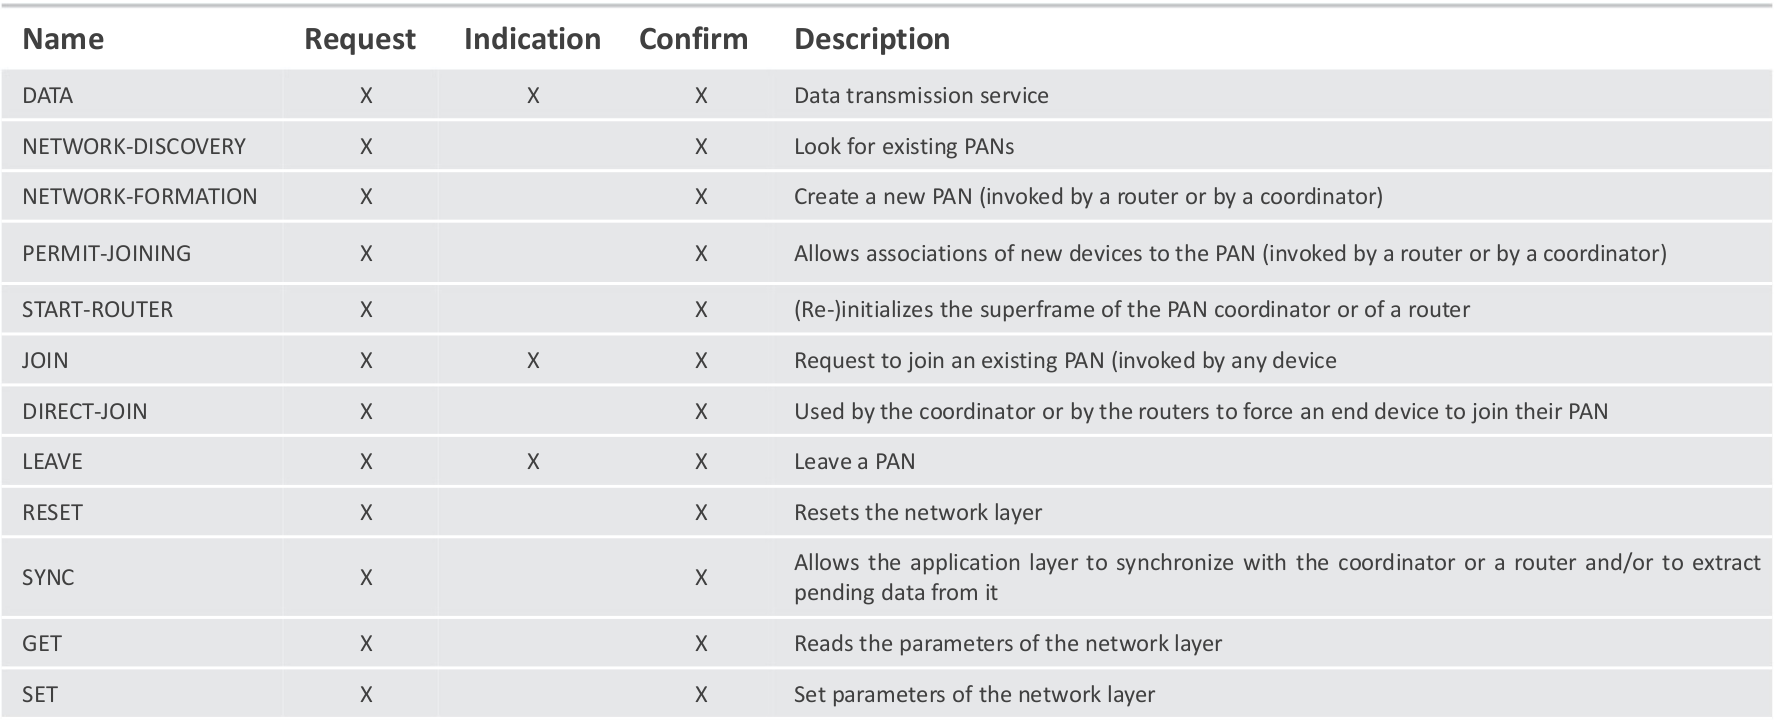
\includegraphics[scale=0.25]{images/Pasted image 20230307165435.png}
	\caption{Operations that exploit the 4 basic primitives}
	\label{table-primitives}
\end{figure}
As highlighted by the table, not all four primitives are used in the listed operations: particularly, the \texttt{GET} and \texttt{SET} are functionalities used \textbf{locally to set/get parameters of the network layer}, internally, without using communication means.

Before communicating over a network, a ZigBee device must either:
\begin{enumerate}
	\item 
	Form a network so it's a \textbf{ZigBee coordinator}
	\item 
	Join an existing network so it's a \textbf{ZigBee router/end-device}
	The role of the device is chosen at \textbf{compile-time} by specifing the code ad application level when writing the \textbf{Application Object} code.
\end{enumerate}


\subsection{Network Formation}\label{sec:network-formation}
The \textit{network formation} is initiated by the \texttt{NETWORK-FORMATION.request} primitive: it's invoked by a device that acts as a \textbf{coordinator} and that is not already in another PAN.
The operation uses the MAC layer services to \textbf{look for a channel} that does not conflict with other existing networks: it \textbf{selects a PAN identifier} which is not alredy in use by other PANs. The process is pictured in \ref{network-formation}

\begin{figure}[h]
	\centering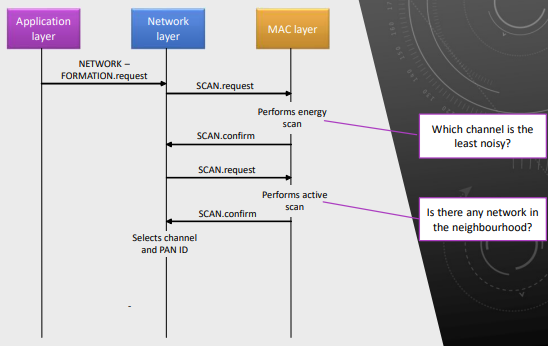
\includegraphics[scale=0.70]{images/Pasted image 20230311120710.png}
	\caption{Network Formation: \texttt{SCAN} request exchange and PAN ID selection}
	\label{network-formation}
\end{figure}


\begin{enumerate}
	\item 
	At application layer is invoked the \texttt{NETWORK-FORMATION.request}
	\item 
	The network layer execute an \textit{energy scan} to verify if there is noisy on the channel
	\item 
	The MAC layer return the result of the energy scan: at this point, the network layer request a second scan, differently from the first because it's an \textbf{actve scan} to lookup nearest PAN networks. This is due to avoid to have two different PAN with the same identifier so a preventive scan allows to select a PAN ID unique among the already existing.
	\item 
	The MAC Layer return a list of existing PAN ID and the Network Layer now can set the PAN ID.
	
\end{enumerate}
The process of \texttt{NETWORK-FORMATION} continues as showed in \ref{network-formation2}
\begin{figure}[h]
	\centering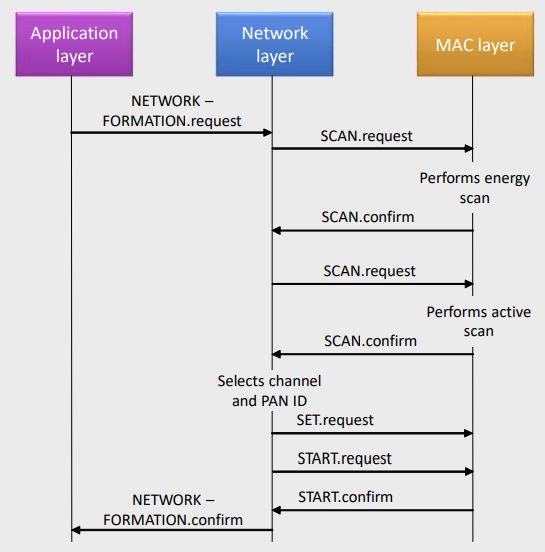
\includegraphics[scale=0.40]{images/Pasted image 20230311121418.png}
	\caption{Network creation confirmation after \texttt{START.request} is completed}
	\label{network-formation2}
\end{figure}

Now the Network layer can configure the MAC layer starting from the time the \texttt{START.request} is sent thus the MAC layer can start to send beacon frames. After that, the MAC layer can answer with a \texttt{START.confirm} that will be translated also by the network layer with a \texttt{NETWORK-CONFIRMATION.confirm}  to the application layer to confirm that the PAN has been created.

\subsection{Device join}
To \textbf{join} inside a PAN network there are two ways:
\begin{enumerate}
	\item 
	The end-device or the router can communicate with the coordinator to request the access: this method is called \textbf{Join Through Association}
	\item 
	The coordinator request a device to join the network: this method is called \textbf{Direct Join} (\textit{no further addressed in this notes})
\end{enumerate}
\paragraph{Join through association (\texttt{CHILD-SIDE})}\label{sec:join-through-association-child-side}
The protocol flow is pictured in \ref{JTA-child-side}
\begin{figure}[h]
	\centering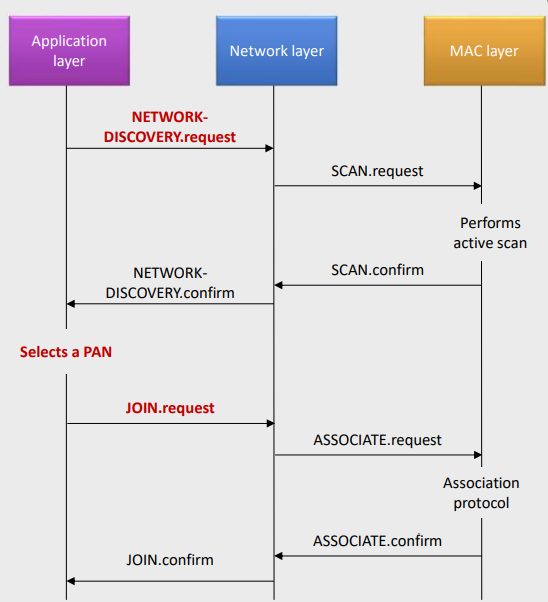
\includegraphics[scale=0.60]{images/Pasted image 20230311121914.png}
	\caption{Join Through Association}
	\label{JTA-child-side}
\end{figure}


The device that wish to join a PAN:
\begin{enumerate}
	\item 
	Performs a \texttt{NETWORK-DISCOVERY} to look for existing PANs
	\item 
	Select a PAN
	\item 
	Invokes \texttt{JOIN.request} with parameters like the \textit{PAN Identifier} of the slected network, a \textit{flag} indicating whether it joins as a router or as an end device. This request in the \textit{network layer} selects a "\textit{parent node \texttt{P}}" (\textit{in the PAN}) from its neighbourhood. In a \textbf{star topology} \texttt{P} is the coordinator and the device join as end-device, while in a \textbf{tree topology} \texttt{P} is the coordinator or a router and the device can join as a router or as an end-device.
	\item 
	The association protocol obtains from \texttt{P} a $16-bit$ \textbf{short address}: the \texttt{ASSOCIATE.confirm} returns to the network layer the short address that will be used in any further communication over the network.
	The \texttt{JOIN.request} is triggered at application level: this require preliminarly to scan the network to find a free channel to communicate. The scan is perfomed troguht \texttt{NETWORK-DISCOVERY} which return a list of PAN network to connect: this allows to select the PAN and send the \texttt{JOIN} request.

\end{enumerate}
	Depending on the three network topologies supported by ZigBee, the \textbf{parent-child} relationship established as a result of \textit{nodes joins} shapes the network in a \textbf{tree} form, where:
	\begin{itemize}
		\item the ZigBee \textit{coordinator} is the \textbf{root}
		\item the ZigBee \textit{routers} are \textbf{internal nodes} \textit{(or even leaves)}
		\item the ZigBee \textit{end-devices} are the \textbf{leaves}
	\end{itemize}
	The \textit{tree-based topology} is exploited by the \textbf{ZigBee Network Layer} to assign the \textbf{short network addresses} based on a specific policy defined by the \textit{ZigBee coordinator}, defined on three main parameters:
	\begin{itemize}
		\item the \textbf{maximum number of routers} \texttt{Rm} that each router may have as a children
		\item the \textbf{maimum number of end-devices} \texttt{Dm} that each router may have as a children
		\item the \textbf{maximum depth of the tree} \texttt{Lm}
	\end{itemize}

	Each router is assigned with a range of addresses to be recursively assigned to its children: devices join as high to the three as possible to \textit{minimize the number of hops}. Despite the addresss are assigned according to a tree structure, the actual network topology can be a \textit{mesh}.
	\begin{figure}[h]
		\centering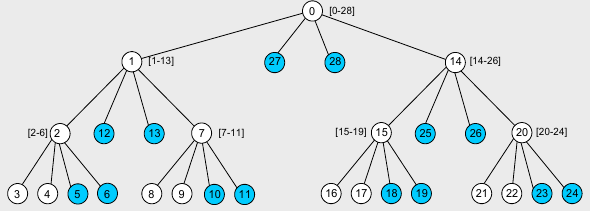
\includegraphics[scale=0.60]{images/Pasted image 20230523172036.png}
		\caption{Address assignment with $Rm = 2, Dm=2, Lm=3$ (\textit{router are white, end-devices are blue})}
		\label{three-based-addressing-assignation}
	\end{figure}\\
In \ref{three-based-addressing-assignation}, the coordinator have index $0$ and considering the left children $1$, the range $[1-13]$ is assigned based on the parameter $Rm, Dm, Lm$, considering the worst-case scenario in which all addresses in this range are used by either a device or a router. The maximum number of nodes (\textit{both end-devices and routers}), in the given example is $28$ because is the threshold given by the three parameter already specified: to have a larger number of nodes it's necessary to set those three parameter to values that allows more nodes. This value limit the number of new devices that can join the network, so new devices cannot enter the network if this limit is reached.\\
This mechanism allows to \textbf{pre-define the set of the addresses to be assigned to joining nodes}: in advance we already know the size of a given subtree (\textit{knowing the max depth and number of children per node}) thus we can allocate the addresses range for each sub-tree.\\
The range assignation is performed following a DFS order, considering sub-nodes children routers (\textit{in \ref{three-based-addressing-assignation}, nodes $2,7$}) range as previously.\\
At network layer we can also define the specific type of \textbf{routing protocol} that ZigBee can use:
\begin{itemize}
	\item 
	\textit{Broadcasting}
	\item 
	\textit{Tree routing}
	\item 
	\textit{Mesh routing}

\end{itemize}
The last two types are for \textit{point-to-point} communication.
\paragraph{Tree routing}\label{sec:tree-routing}
Consider the scenario pictured in \ref{tree-routing-scenario}.
\begin{figure}[h]
	\centering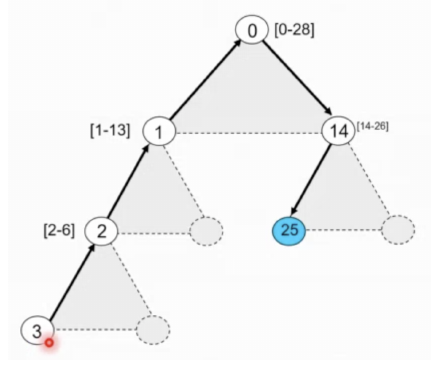
\includegraphics[scale=0.50]{images/Pasted image 20230524141226.png}
	\caption{Tree routing scenario}
	\label{tree-routing-scenario}
\end{figure}

The node $3$ that want to communcate with node $25$ must forward the packet to node $2$ because is his father. The node 25 is outisde of node 2's range so the packet will be forwarded to node $1$ and again to node 0 which is the root node. The packet will be forwarded to 14 and then to node 25.
All those communciation happen between routers, except the final one that is between the router 14 and the end-device 25: for the last hop, the node 14 can advertise the node 25 of the presence of a new message in its \textit{beacon message}, so the node 25 will request the message itself to node 14.
\paragraph{Mesh routing}\label{sec:mesh-routing}
It's based on \textit{AODV protocol} (\textit{which is not in the scope of the following notes}): the key idea is that each router have its own routing table, mantaining destination, next hop and a set of information about the path to a specific node.

\begin{figure}[h]
	\centering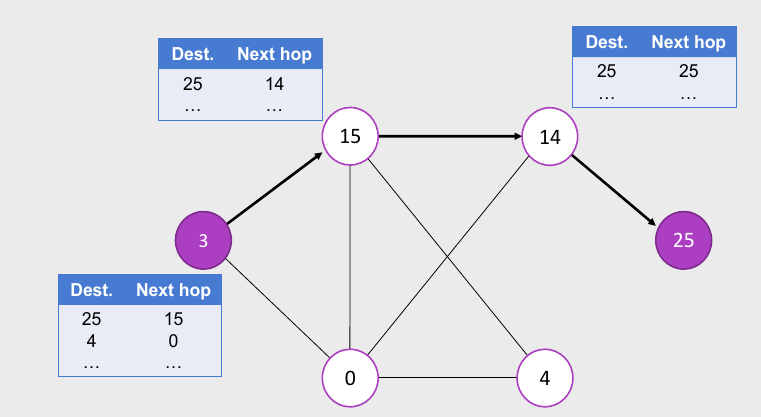
\includegraphics[scale=0.50]{images/Pasted image 20230524141323.png}
	\caption{Mesh routing scenario}
\end{figure}

If the communication happen between the node 3 and node 25, the source node will verify that the destination exists in an entry of its routing table: if the entry does not exists, a \textbf{path discovery} operation is triggered.
The path discovery operation exploit the \textit{broadcast} method, containing the \textit{request ID} and the \textit{path cost}, initialized to 0: the request is propagated inside the network so each intermediary router can answer if an entry with the target destination is found in one of the node's routing table.


	
	
	
	
	
\subsection{Application Layer}\label{sec:application-layer}
The application layer comprends various components (\textit{as shown in \ref{zigbee-app-layer}}):
\begin{figure}[h!]
	\centering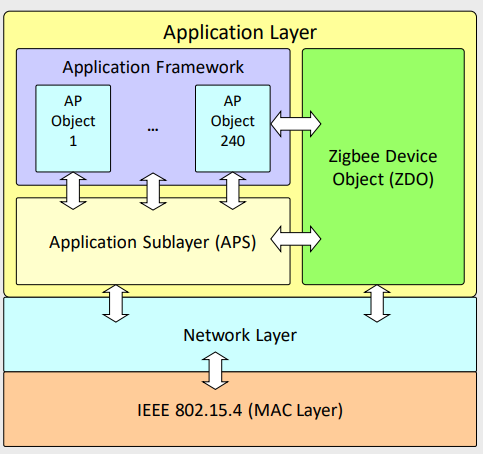
\includegraphics[scale=0.50]{images/Pasted image 20230311122809.png}
	\caption{ZigBee Application layer segmentation in three sub-layers and interaction with network layer}
	\label{zigbee-app-layer}
\end{figure}

\begin{enumerate}
	\item 
	\textbf{Application Framework}: contains up to 240 \textbf{Application Objects (APO)} in which each APO is a user defined ZigBee application.
	\item 
	\textbf{ZigBee Device Object (ZDO)}: provides services to let the APOs organize into a distributed application. Guarantee interoperability between different devices of different vendors
	\item 
	\textbf{Application Support sublayer (APS)}: provides data and managemnt services to the APOs and ZDO.
\end{enumerate}
\subsection{1. Application Framework}\label{sec:1-application-framework}
The application framework can contains up to 240 different \textit{Appication Object (APO)}, each one uniquely identified inside the netowrk.
Simplest APO can be queried with \textit{Key Value Pair data service (KVP)} by using primitives like \texttt{Set/Get/Event} transactions on the APOs attributes: native KVP disappeared in the second version of ZigBee but it’s now present in the cluster library.
Complex APO can have conpelx states and communicate with the \textit{Message data Service}. \\\\
 In figure \ref{APO-ex1} an example of complex APO: we have two devices, the first with two endpoint, the second with three endpoint. The logic of this device can be easily implemented using two \texttt{ON-OFF} attribute and two endpoint in the device A.
\textbf{APOs 5B, 6B, and 8B} have a single attribute containing the status of the bulbs (on/off) that is configured as servers at the application layer while \textbf{APO 10} and \textbf{APO 25} are switches, and they are configured as clients at the application layer. The attributes of \textbf{APOs 5B, 6B}, and \textbf{8B} can be set remotely from the \textbf{APOs 10A} and  \textbf{APO 25A}.

\begin{figure}[h]
	\centering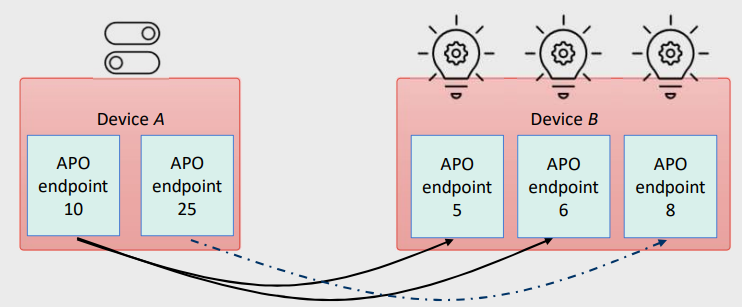
\includegraphics[scale=0.40]{images/Pasted image 20230311123327.png}
	\caption{APO bulbs example}
	\label{APO-ex1}
\end{figure}


\subsection{2. Application Support Sublayer (APS)}\label{sec:2-application-support-sublayer-aps}
The APS define the \textbf{endpoint, cluster, profile IDs and device IDs}. It's responsible for:
\begin{itemize}
	\item 
	Data service (\textit{light transport layer}) that provides support for the communication's reliability and packet filtering
	\item 
	Management services which includes mantaining a local binding table, a local group table and a local addresss map.
\end{itemize}

The \textbf{endpoints} are identified by a number between 1 and 240: an endpoint can be seen as the equivalent of a Unix socket, connecting virtual wires to applications.
The \textbf{cluster} is a protocol that can be used to implement the functionality of a given application: cluster defines the attribute that contains the information about the APO. A cluster is defined by a \textbf{clusterID} of \textit{\textbf{16 bit}} (\textit{as shown in \ref{cluster-table}}), local inside the \textbf{profile}. In ZigBee a \textbf{profile} defines a set of application layer protocols that enable interoperability between devices that perform specific functions or serve specific purposes. A profile specifies the standard ways in which devices should communicate and exchange information, making it easier for devices from different manufacturers to work together.

A profile consists of one or more \textbf{clusters}, which are groups of related functionality that can be supported by a device.

A cluster defines a specific set of \textbf{messages and commands} that devices can use to communicate with each other. \textit{For example}, the ZigBee Home Automation profile includes clusters for controlling lights, thermostats, and door locks. Each cluster specifies the \textbf{data format and message types} that devices should use to exchange information related to that functionality.
\begin{figure}[h]
	\centering
	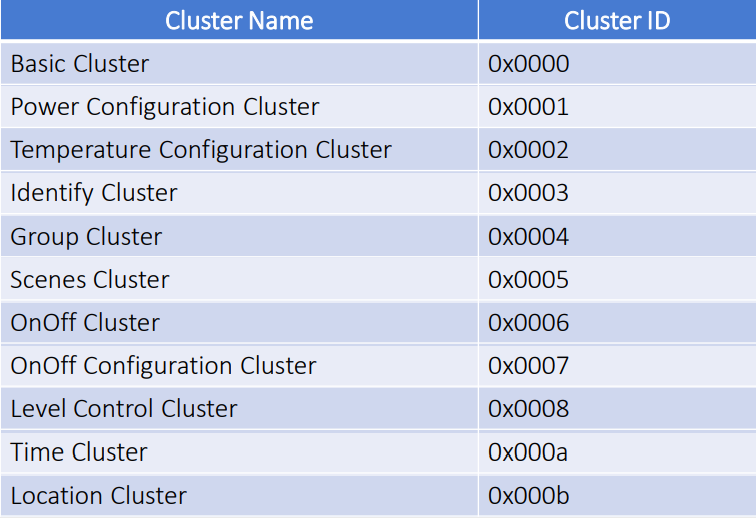
\includegraphics[scale=0.50]{images/Pasted image 20230311124737.png}
	\caption{Prefefined clusters ID}
	\label{cluster-table}
\end{figure}

In the previous table, the \textit{Basic Cluster} with ID \texttt{0x0000} allows to retrieve basic information about the device, the \textit{Power Configuration Cluster} allows to set the \textit{minimum and the maximum temperature} of the device. Also, the \textit{OnOff Cluster} allows to set the \textit{switch} ON or OFF, as expected.\\\\
The \textit{APS \textbf{Device IDs}} range from \texttt{0x0000} to \texttt{0xFFFF}, this value has two main purposes:
\begin{enumerate}
	\item 
	To allows human readable displays (\textit{e.g. an icon is realted to a device})
	\item 
	Allows ZigBee tools to be effective also for humans: a device may implement the on/off cluster but you don't know whether it's a bulb or a oven so you only kwno you can turn it on or off. The DeviceID tells you what it is, but it does not tell you how you can communciate with it: this is given by the IDs of the cluster it implements.\\
	ZigBee discovers services in a network based on profile IDs and cluster IDs, but not on device IDs alone because each device is specified by the combination of Application profile ID and cluster ID.
	
\end{enumerate}
In figure \ref{cluster-IDs} an example of cluster IDs.
\begin{figure}[h]
	\centering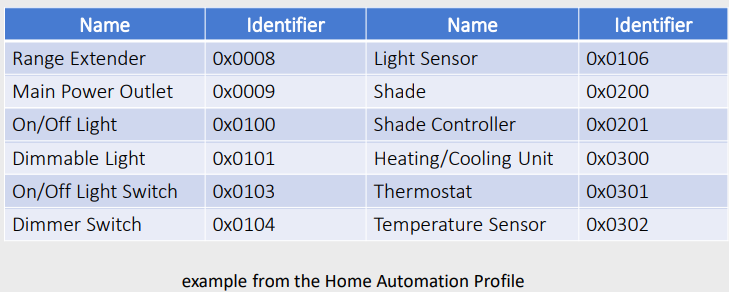
\includegraphics[scale=0.50]{images/Pasted image 20230311161838.png}
	\caption{Cluster ID example}
	\label{cluster-IDs}
\end{figure}
\subsubsection{APS Services}
The \textbf{APS \textit{\textbf{Services}}} provides data service to both APOs (\textit{Application Objects}) and ZDO (\textit{ZigBee Device Object}), allowing to \textit{\textbf{bind a service to the ZDO}} and \textit{\textbf{group management services}} (\textit{see later)}. APS data service enables the exchange of messages between two or more devices within the network: here the data exchange is defined in terms of primitiviles like \texttt{request(send), confirm(return status of trasnmission), indication(receive). }

The reliability of a data service is ensured by using the \textbf{ACKNOWLEDGE messages} for data trasmission as the schema \ref{zigbee-data-ack} indicates.
\begin{figure}[h!]
	\centering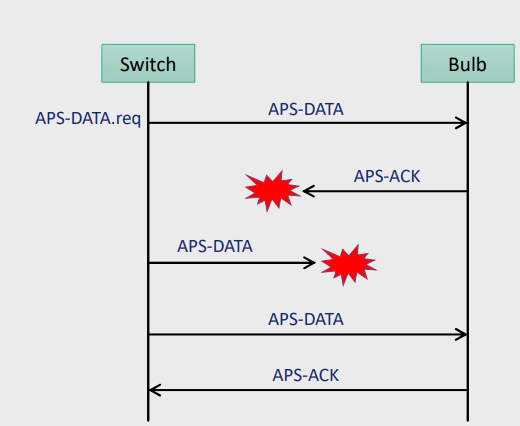
\includegraphics[scale=0.50]{images/Pasted image 20230311162150.png}
	\caption{APS exchange diagram}
	\label{zigbee-data-ack}
\end{figure}


The \textit{\textbf{APS Group Management}} provides service to build and mantains groups of APOs: a group is identified by a $16-bit$ address and each APO in the group is identified by the pair network \textit{address/endpoint}. The \texttt{ADD-GROUP} primitive allows to add an APO to a group and \texttt{REMOVE-GROUP} primitive to remove an APO from a group: takes group number and endpoint number; if the group does not exists it's created. The information about groups are stored in a \textit{group table} in APSs.

\subparagraph{APS Binding}\label{sec:aps-binding}
The binding operation allows an endpoint on a node to be connected (\textit{bound}) to one or more endpoints on another nodes: the binding is \textbf{unidirectional} and can be configued only by te ZDO of the coordinator or of a router. \\
So the binding provide a way to specify the destination address of the messages. This method is called \textbf{Indirect Addressing}: when a Message is routed to the destination APO based on its pairs \texttt{<destination endpoint, destination network address>} the method is usually called \textbf{Direct Addressing}. Direct addressing might be unsuitable for extremely simple devices while \textit{Indirect addressing} exploit the \textit{\textbf{Binding table}}.

Two main primitives are used for binding in \textbf{Indirect addressing}, respectively \texttt{BIND} and \texttt{UNBIND}:
\begin{enumerate}
	\item 
	\texttt{BIND.request} creates a new entry in the local binding table. It takes in input the tuple 
	\begin{center}
		\texttt{<source address, source endpoint, cluster identifier, destination address, destinatione endpoint>}
	\end{center}
	
	\item 
	\texttt{UNBIND.request} deletes an entry from the local binding table
\end{enumerate}

In the \textbf{Indirect addressing}, the binding table matches the \textit{source address \texttt{<network addr, endpoint addr>}} and the \textit{cluster identifier} into the pair \texttt{<destination endpoint, destination network address>}. The binding table is stored in the APS of the ZigBee cordinator and/or of the other router: it's updated on explicit request of the ZDO in the routers on in the coordinator. It's usually initialised at the network deployment.

In the scenario of light bulb and a switch, can be complex from the switch side to know to which light bulb connect but, this information is known by the installer. Despite operating directly on the device, the installer can set and entry in the \textbf{coordinator's binding table} so that the messages arriving to the switch will be forwarded to the light bulb.

Here an example of \textbf{binding table} with a request \texttt{APS-DATA.req} of cluster 6 from endpoint 5 on node \texttt{0x3232} that in \textbf{indirect routing} will generate 4 data requests:
\begin{itemize}
	\item 
	Node \texttt{0x1234}, endpoint \texttt{12}
	\item 
	Multicast to group \texttt{0x9999}
	\item 
	Node \texttt{0x5678}, endpoint \texttt{44}
\end{itemize}

\begin{figure}[h]
	\centering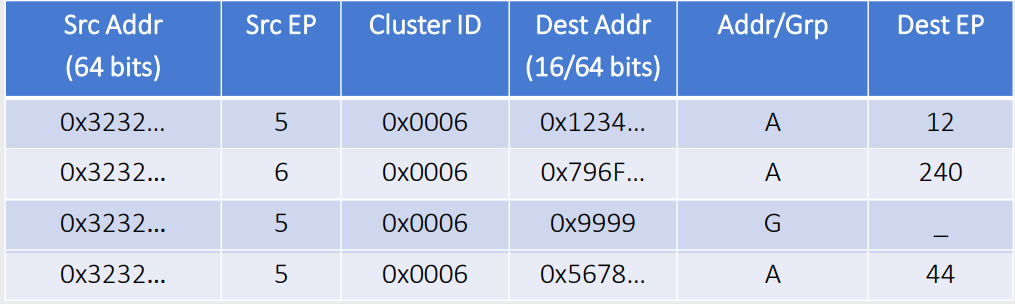
\includegraphics[scale=0.30]{images/Pasted image 20230311163416.png}
	\caption{Binding table example}
	\label{zigbee-binding-table}
\end{figure}

In the binding table showed in \ref{zigbee-binding-table}, the \texttt{Src Addr} and the \texttt{Dest Addr} are formatted as a MAC addresses: this choice has been made because the devices can disconnect/re-connect to the network for many reasons, requiring a reconfiguration of the addresses in the binding table.
The column \texttt{Addr/Grp} allows to tag as destination a group of devices (\texttt{G}). Also, the same devices can be the source of different messages (\texttt{Src EP = Endpoint}).

The \textit{APS \textbf{Address Map}} \ref{zigbee-addr-map} allows to associated the $16-bit$ network address with the $64-bit$ IEEE MAC address: ZigBee end devices (\textit{ZED}) may change their 16 bit network address when they leave and join again. In that case, an announcement is sent on the network and every node updates its internal table to preserve the binding.
\begin{figure}[h]
	\centering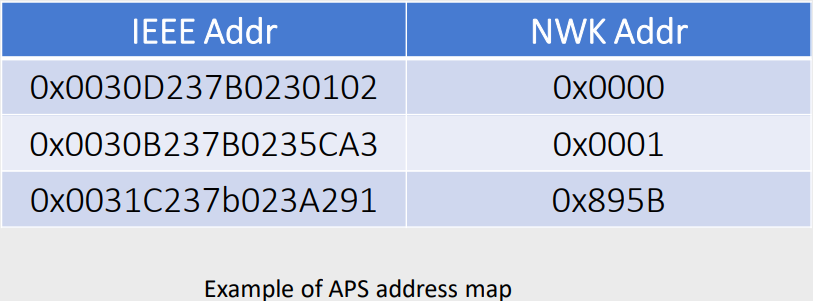
\includegraphics[scale=0.30]{images/Pasted image 20230311163736.png}
	\caption{Address map example}\label{zigbee-addr-map}
\end{figure}



\subsection{3. ZigBee Device Object (ZDO)}\label{sec:3-zigbee-device-object-zdo}
ZDO is a \textit{special application} attached to \textit{\textbf{endpoint \texttt{0}}}: it implement the basic functionalities expected by the devices. It also implement the end-device or router or coordinator based on the specific configuration given by the \textbf{ZigBee Device Profile} that describe the cluster that must be supported by any ZigBee device, defines how the ZDO implements the services of discovery and binding and how it maanges the network and security.\\
So the main ZDO services are \textit{device and service discovery, binding management, network management, node management}.

\subsubsection{Device and service discovery}\label{sec:device-and-service-discovery}
The \textbf{ZigBee Device Profile} specifies the device and the \textit{service discovery mechanisms} to obtain any information about devices and services in the network. The \textbf{Device Discovery} allows a device to obtain the (\textit{network or MAC}) address of other devices in the network: starting from an unknown address it allows to identify the relative device inside the network. It follow an \textbf{hierarchical implementation} in which a router return to its parent its address and the address of all the end-devices is associated to itself. Then the coordinator returns the address of its associated devices.\\
A newly joined device does not know anything about the network: to provide a service it must also known, require and use the services offered  by other devices. This actions are performed thanks to \textbf{ZigBee Device Profile} that allows the service discovery of other devices.\\
The service discovery send queries that are based on \textit{cluster ID, profile ID} and optionally on \textit{service descriptors}: the coordinator responds to service discovery query by returning lists of endpoint addresses matching with the query. The hierarchical implementation is effective because \textit{each router collect information from its associated devices and forwards it to its parent}.\\\\
The other mechanism to understand what service a device is providing is called \textbf{Service Discovery}: the network is created according to a parent-child relation (with a coordinator), building as a tree (\textit{as the addresses tree previously mentioned}). To known which service a device offer, a joined device ask to its coordinator that may not have fully all the information and may ask to it's parent node, recursively. Each node is responsible for the subtree under its domain: in case of missing information, intermediate routers prepare information report to answer the queries.\\
The \textbf{Service Discovery} provides a report that tells for a single device what are the cluster to which it responds: for example, a device can responds telling that implement a ON/OFF cluster. The service discovery can be direct to the coordinator and is it's responsability to collect information and answer for the whole network.
The requests can be directed also to end-device but due to low-power devices, they may not be ready to answer the queries regarding the services they offer.
The service discovery does not tell where the device is physically located, only the service offered and their relative identifier (Cluster ID, Device ID, etc): to obtain the location is necessary that a device implements the \textbf{Identity Cluster} that force a device to identify itself by blinking a led.
\subparagraph{Binding management}\label{sec:binding-management}
The ZDO processes the binding requests received from local or remote EP: both to add entries and delete entries from the APS binding table (\textit{by invoking primitives}). This process require having an IEEE address.
\subparagraph{Managing network and nodes}\label{sec:managing-network-and-nodes}
The \textit{network management} implements the protocols of the coordinator, a router or an end-device according to the configuration settings established either via a programmed application or at installation. Differently, the \textit{node management} involves the ZDO to serves incoming requests aimed at perfoming network discover, retrieving the routing and binding tables of the device and managing \texttt{join/leaves} of nodes to the network.

\subsection{ZigBee Cluster Library (ZCL)}\label{sec:zigbee-cluster-library-zcl}
The ZCL is a repostory for cluster functionalities: it's a \textit{working library} with regular updates and new functionalities. The develoeprs are expected to use the ZCL to find relevant cluster funcionalities to use for their application.
The main goal is to avoid re-inventing the wheel, supports \textbf{interoperability} and facilitates maintanability: two devices must implement the same application layer to use each other. The ZCL allows to implement the same set of commands and functionalities, standardized by ZCL.\\
For example, in a \textit{base home automation system} we have many application execute at the same moment: the ZCL allows to specify the behaviours of the involved devices based on a \textit{\textbf{client-server model}}.\\\\
A \textbf{cluster is a collection of commands and attributes}, which define an interface to a specific functionality.
The \textbf{device} that stores the attributes, by keeping an internal state, is the \textbf{server of the cluster} while  the device that manipulates/writes the attributes is the \textbf{client of the cluster}.
It's not necessary that a server have more computational power than end-devices.
\begin{figure}[h!]
	\centering\includegraphics[scale=0.40]{images/Pasted image 20230311165232.png}
	\caption{Client-server cluster binding operation}
\end{figure}

If we think an application that switch the light, it will have an attribute \texttt{ON/OFF} and the client will be the switch that turn on/off the light while the server will be the light bulb itself.
Cluster are grouped in \textbf{functional domains}:
\begin{itemize}
	\item 
	\textit{General}: allows the access and control of any device, irrespective of their functional domain. Includes general basic functions, implemented by all devices.
	\item 
	\textit{Closures}:  for shade controllers, door locks.
	\item 
	\textit{HVAC}: for pumps (\textit{like fan, heating, etc})
	\item 
	\textit{Lighting}: control lights
	\item 
	\textit{Measurement and sensing}: illuminance, presence, flow, humidity
	\item 
	\textit{Security and Safety}: security zone devices (\textit{e.g. passive infrared})
	\item 
	\textit{Protocol interfaces}: interconenct with other protocols
	
\end{itemize}
Each functional domain, for each server, defines \textbf{commands} and \textbf{message structure}.
The \textbf{commands} are messages (\textit{with their own header and paylaod}) with a format specified by ZCL: the commands can be read/write attribute or also can be used for dynamic attribute reporting (\textit{useful to periodic reading of the sensors}).
The \textit{types of command} are generally three:

\begin{enumerate}
	\item 
	Read/write an attribute
	\item 
	Configure a report and read a reporting response:  allows to request periodic attribute/configuration reading. Requests for report whenever an attribute/configuration changes. The client ask the server to report periodicly about the state of the server: the server will send periodically a report to the client, withoyt any further request. Also defines parameters of the reporting like \textit{duration, period, minimum change, etc}.
	\item 
	Discover attributes: to discover the IDs and types of the attributes of the cluster that are supported by the server
\end{enumerate}

The \textit{schemes of use} \ref{zcl-use-scheme} show a typical use of \textbf{device configuration and installation cluster:} the configuration phase allows to setting up some parameters by using several clusters.
The \texttt{Basic} domain allows to retrieve software version, manufacturer ID, etc. The \texttt{PowerConfig} return information about battery and power configuration. The \texttt{Temperature Configuration} allows to set treshold, etc. Last, the \texttt{Identify} cluster allows to identify physically a device.
\begin{figure}[h]
	\centering\includegraphics[scale=0.40]{images/Pasted image 20230311165919.png}
	\caption{Common functional domains use between client and server}
	\label{zcl-use-scheme}
\end{figure}

Following the schema, usually the installer configure the devices by using specific configuration tools that allows to connect to the devices, apply the specific settings and read their status. As an example, the \texttt{Identify} allows to recognize the device by enabling a blinking led.\\
Applied to our \texttt{ON/OFF} previous example, the relative scheme obtained is pictured in \ref{zcl-on-off-ex}
\begin{figure}[h!]
	\centering\includegraphics[scale=0.45]{images/Pasted image 20230311165957.png}
	\caption{Lamp switches configuration diagram and interconnection}
	\label{zcl-on-off-ex}
\end{figure}\\
In this case we want to configure a set of APO, we have one
ON/OFF switch which is connected with a "\textit{Simple Lamp}", we have to
create the association between the lamp and the switch, in the same way we must also create the association between the "dimmer switch" and the "dimmable lamp".\\\\
This association is created by the \textbf{Configuration Tool}, working as a client sets the configuration of the On/Off switch device in such a way that when it wants to turn the lamp on or off it will find the corresponding device and make the request for turning on or off. The same goes for configuring the Dimmer Switch. The configuration tool must also configure the simple lamp. The configuration allows to setup the \textbf{binding table} to the \textbf{coordinator} by knowing the addresses of the devices and relative APO. This can be done by invoking device and service discovery, alongside physical discovery.\\
Typically what happens is that the installer has a tablet and it connects to the Zigbee Network, using an application you can access information about the network. When I run this configuration each device knows what it is and what it can do, a lamp for example knows it is a lamp but it is necessary to carry out a \textbf{commissioning procedure} so that the lamp is connected to an on/off switch which allows the ignition. It's necessary to execute the procedure of \textit{commissioning} to simplify the deployment of complex smart system, like in a scenario with hundreds of devices to be deployed and configured.\\
Each devices has many of information assigned to it, contained in the \texttt{BASIC} cluster, like the ones listed in \ref{basic-cluster-info}.
\begin{figure}[h!]
	\centering\includegraphics[scale=0.30]{images/Pasted image 20230311170348.png}
	\caption{\texttt{BASIC} cluster information}
	\label{basic-cluster-info}

\end{figure}\\
The \texttt{ZCLVersion} is mandatory to be sure that the ZCL is the right one implemented at application level, specially due to continue updating.
Also the  \texttt{PowerSource} is mandatory because provide information about power sources. Usually the  attributes in \texttt{BASIC} cluster are in \textit{read-only} access.\\
Among those information, highly relevant are the \texttt{PowerSource}, an 8-bit number that can have the values listed in \ref{powersource-values}. 
\begin{figure}[h!]
	\centering\includegraphics[scale=0.20]{images/Pasted image 20230311170452.png}
	\caption{\texttt{PowerSource} attribute}
	\label{powersource-values}

\end{figure}\\
The value in the last table indicates the \textbf{type of battery}, if there is an emergency power supply, etc. Those devices have also the attribute called \textbf{tempetature measurement cluster} that allows to kown the tempetature \textit{inside} the device itself.
The attribute to know this temperature are specified by \texttt{Temperature} cluster as listed in \ref{temperature-cluster}.
\begin{figure}[h]
	\centering\includegraphics[scale=0.30]{images/Pasted image 20230311170646.png}
	\caption{Temperature cluster data definition}
	\label{temperature-cluster}

\end{figure}

The cluster specified uses only generic commands to \textit{read attributes, discover attributes, configure and report.} There are no specific commands to program a simple devices as a temperature measurement.For complex devices that also implement part of the \texttt{Temperature} cluster there is usually an accessory appendix that specify other commands.\\
ZCL is designed to enforce a hierarchical approach  to device functionality by supporting backward compatibility and interoperability, as shown in \ref{zcl-interop}: instead of design every possible ZCL cluster for specific \textit{lamp}, it's incremental and allows compatibility by also let the possiblity to create custom features not standardized by ZigBee.
\begin{figure}[h!]
	\centering\includegraphics[scale=0.30]{images/Pasted image 20230311171010.png}
	\caption{Hierarchical approach for lamp example}
	\label{zcl-interop}
\end{figure}

\subsection{ZigBee Security Specification}\label{sec:zigbee-security-specification}
Security services provided for ZigBee include methods for:
\begin{enumerate}
	\item 
	Key Establishment: create the keys without prior information
	\item 
	Key Transport: exchange keys previously setted/stored at configuration time
	\item 
	Frame Protection: by using encryption
	\item 
	Device Management
	
\end{enumerate}
Security services are optional and have an overhead, minimum for low power devices. These services form the building blocks for implementing security policies within a ZigBee device.\\
The underlying assumptions are that \textbf{level of security} depends on:
\begin{itemize}
	\item 
	the safekeeping of the symmetric keys: by avoiding stolen information about keys, also physically
	\item 
	the protection mechanisms employed,
	\item 
	the proper implementation of the cryptographic mechanisms and associated security policies involved.
	\textbf{Trust} in the security architecture comes from:
	\item 
	trust in the \textit{\textbf{secure initialization}} and installation of keying material and
	\item 
	trust in the \textit{\textbf{secure processing and storage}} of keying material.
\end{itemize}

Further assumptions are:
\begin{itemize}
	\item 
	\textbf{correct implementation of all security protocols}: the  implementation must follow the standard, according to ZigBee standard and deployment operations
	\item 
	correct random number generators
	\item 
	secret keys do not become available outside the device in an unsecured way. The only exception to this is when a device joins the network.
\end{itemize}

Due to the \textit{low-cost nature of ZigBee devices} we \textbf{cannot generally assume the availability of tamper resistant hardware}: it's possiible to some extent but it's not provided by the ZigBee standard (\textit{can be possible by anti tamper hardware up to a given point}).  The level of protecntion is both at network level of physical level.  Hence, physical access to a device may yield access to secret keying material and other privileged information, as well as access to the security software and hardware. Also, \textbf{different APO in the same device are not logically separated and lower layers are entirely accessible to the application layer}. Hence different APO in the same device must trust each other.
\subparagraph{Security Design Choices}\label{sec:security-design-choices}
The security is granted by the \textbf{Trust Center} that it's a module in the \textit{Application Layer}, tipycally allocated in the \textit{ZDO} that distribute the security keys to the devices inside the same network.
Two main keys are provided, at different level:
\begin{itemize}
	\item 
	\textbf{Single key per network} (\textit{network level security}): each Zigbee network is assigned a unique network key, which is a symmetric encryption key. This network key is shared among all devices within the network and is used to encrypt and decrypt data transmitted between them. Since it is a symmetric key, the same key is used for both encryption and decryption.
	\item 
	\textbf{Single key per link} (\textit{device-to-device level security})
	The process flows: the devices inside the network uses a \textbf{Master key} to connect to the \textbf{Trust center}: this master key can be pre-assigned to the device (\textit{write in ROM/Firmware}) or can be injected later in the device. The master key allows to establish a connection to request  the \textbf{Network keys} or \textbf{Link keys}. \\ 
	Those three key allows ZigBee to provide a level of encryption corresponding to $AES-128$ that it's enough for low power devices. The keys are provided by the APS. The low power and computing constraints of the devices implies that the encryption is \textbf{symmetric} and the decryption is made by the keys provided by the \textit{application layer}.
	It aims to the protection of individual devices but not individual applciations in the same device: this allows the re-use of the same keying material among the different layers of the same device.
\end{itemize}

The layer that originates a frame is responsible for initially securing it: if a network command need protection this must be ensured at network level security. If protection from \textit{theft of service} is required, network layer security must be used for all frames (\textit{except the one when new device joins}). The reuse of key materials among different layers in a device and link-keys allows to have additional security from source to destination: an application can extends the security by adding other mechanism but it's entirely upon itself.

An \textit{application profiles} should include policies to:
\begin{itemize}
	\item 
	Handle error conditions arising from securing and unsecuring packets: error conditions may indicate loss of synchronization of security material or may indicate ongoing attacks.
	\item 
	Detect and handle loss of counter synchronization and counter overflow.
	\item 
	Detect and handle loss of key synchronization.
	\item 
	Expire and periodically update keys, if desired.
\end{itemize}
\paragraph{The keys}\label{sec:the-keys}
The keys can be obtained by means of:
\begin{itemize}
	\item 
	\textbf{Key transport}: a mechanism for communcating a key from one device to another dervice or other device. It's a sensible phase because at that time the communication is unencypted: can be encrypted but with more overhead, depending the scenario context.
	\item 
	\textbf{Key establishment}:  a mechanism that involves the execution of a protocol by two devices to derive a mutually shared secret key
	\item 
	\textbf{Pre-installation}: at manufacturing time, install the key into the device or during the deploying phase
\end{itemize}

The \textbf{Network key} are \textit{128-bit} shared by all devices: they are acquired either by key-transport or pre-installation and generally are of two types (\textit{\textbf{standard vs high security}}).\\
The \textbf{Link keys} are 128 bit, shared by all devices: they are acquired by key-transport, key-establishment or pre-installation. The key establishment is based on pre-existing master key. Two types are considered (\textit{\textbf{Global vs Unique}}).\\
The \textbf{Master key} is a 128 bit key acquired either by key transport or pre-installation. Other keys are used to implement the secure transport of key material: they are derived from the link key with one-way functions.\\\\
The \textbf{Key Establishment} it's stated by the specification: it describe a variation of Diffie-Hellmann and it's called \textbf{SKKE (Symmetric-Key Key Establishment)}. Usually the key establishment involves two entities, an initiator device and a responder device. It evolves as following:
\begin{enumerate}
	\item \textit{trust provisioning based on trust information (typically the master key)}: the master key can be either pre-installed during manufacturing or it may be installed by a Trust Center (\textit{for example, from the initiator, the
	responder, or a third-party device acting as a Trust Center}), or it may be based on user-entered data (\textit{for example: PIN, password, or key})
	\item exchange of ephemeral data (a random number)
	\item  the use of this ephemeral data to derive the link key.
	\item  confirmation that the link key was computed correctly
	
\end{enumerate} 
The \textbf{Trust Center} is the device trusted by devices within a network: it's a funcionality implemented in the coordinator or a specified device. In a simple network can be the coordinator and it's usually used to obtain new \textbf{network/link key} by connecting to it and requesting new keys. All members of the network shall recognize exactly one Trust Center and  there shall be only one in each secure network to provide a trust agreement between all the device in the same network.\\
The device that joins the network:
\begin{itemize}
	\item obtain the keys from the trust center according to different protocols, depending on which keys they already have (or no key) 
	
	
	\item in low-security applications the Trust Center give it the master key
	by using unsecured transport 
	
	\item If the device already has the master key, it can establish a secure
	communication link with the Trust Center to transport the keys.
	
\end{itemize}


\chapter{IoT Design Aspects}\label{sec:iot-design-aspects}
IoT are special custom devices that need to manage the energy efficiency differently from standard market device.
The devices we refer are usually charaterized by \textit{low power, low cost, small size} and \textit{entirely autonomous}, being able to perform operative operations without the human intervention.

Each device is a full micro-system that embeds:
\begin{itemize}
	\item 
	Processor
	\item 
	Memory
	\item 
	Radio transceiver
	\item 
	Battery powered or energy harvesting methods: depending on the specific scenario, both allows to avoid wired powered devices.
\end{itemize}

The \textbf{energy efficiency} based on battery-powered implies that the working life is limited in time: this implies the need to intervene on the field to change the battery. This operation can be costly, respect to the device cost itself.
Some other issues are \textit{adaptability to changing conditions} that arises for dynamic network management and programming, adapting its behavior as the environment change. This implies the necessity of \textit{dynamic programming} to also preserve the interoperability.\\
Another problem is that the devices comes in term of very \textit{low complexity and overhead}, with reduced complexity of operation execution and constrains on computational resources.
Another issues concerns \textit{multi-hop communication}: standard routing protocols like Distance Vector or similar relies on address table but due to constrained capacity both in term of storage and computational resoures, those model does not scale in IoT context multi-hop network.

This also introduce the problem of the \textit{mobility} that need for dyamic routing protocols to scale efficiently, provided the underlying infrastructure.

\subparagraph{Moore's Law}\label{sec:moores-law}
\textit{"The number of transistor that can be embedded in a chip grows exponentially (it doubles every two year)"}.
The application of Moore's law to IoT is peculiar and subject to different interpretation, like: 
\begin{enumerate}
	\item 
	The \textit{performance doubles every two years} at the same cost
	\item 
	The \textit{chip's size halves} every two year at the same cost
	\item 
	The size and the processing power remain the same but the cost halves every two year.
	
\end{enumerate}
In IoT all those interpretation are true, based on the specific scenario: there are application that require small sized sensors and or that have low power comsuption, can require higher processing capabilities. There is the need to balance the computational power to the costs, based on the specific application.\\
The Moore's law does not necessarily solve the problem in IoT design, at least in the near future.
\section{Energy efficiency}\label{sec:energy-efficiency}
It represent one of the critical aspects because devices are usually battery-powered, avoid wired powered devices and avoid maintenance cost.
The energy efficiency is one of the main aspects in IoT design: the following diagram shows how the evolution of \textit{processor, HD capacity and memory} grows faster than battery efficiency as pictured in \ref{processor-vs-capacity}
\begin{figure}[h]
	\centering\includegraphics[scale=0.50]{images/Pasted image 20230324162428.png}
	\caption{Processor and memory storage evolution over the years}
	\label{processor-vs-capacity}
\end{figure}
The improvements of the battery efficiency is not bound to the Moore's Law: this is also due to the physic limit. The consequences are that if we want to improve the battery efficiency, we need to improve the design aspects of an IoT system, improving the design of the components that heavily rely on battery.

In a laptop, most of the energy in spent on a screen, as shown in \ref{laptop-usage} image.
\begin{figure}[h]
	\centering\includegraphics[scale=0.50]{images/Pasted image 20230324162704.png}
	\caption{Energy expenditure for a commercial laptop}
	\label{laptop-usage}
\end{figure}

In a wireless sensor, the energy usage follows a different pattern than in laptop as pictured in \ref{iot-usage}: 20\% of battery is used for sensing activities, the 40\% is used for wireless and network interfaces activities and the remaining part, about 40\%, is used by the processor and the chipset.
\begin{figure}[h!]
	\centering\includegraphics[scale=0.50]{images/Pasted image 20230324162732.png}
	\caption{Energy expenditure for a commercial IoT device}
	\label{iot-usage}
\end{figure}

The percentage areas can vary based on the specific sensors. There is a trade-off between sensing and transmission: \textit{"a general rule state that transmit 1 byte is equal to compute 1k byte"}.
Usually the sensing activation frequency it's mandatory based on a given context: reducing it have a direct impact on the quality of sensing data. The opmitizable component is surely the \textbf{processor area} but, differently, the sensing area cannot be opmitized muchly because it both transmit and receive: the optimizable part is the one that concern the communication timeframe and behavior.
A radio for \textbf{WiFi Network Interface} can be in 4 modes, each with different energy consumption:
\begin{enumerate}
	\item 
	\textbf{Sleep Mode}: consume very less and can get the radio operative in short time. The energy consumption is around $10mA$.
	\item 
	\textbf{Listen Mode}: $180mA$
	\item 
	\textbf{Receive Mode}: $200mA$
	\item 
	\textbf{Transmit Mode}: $280 mA$
\end{enumerate}

For a sensor (\textit{specifically the moto-clone}) the energy consumption is:
\begin{enumerate}
	\item 
	Sleep Mode:  $0.16mW$
	\item 
	Listen Mode:  $12.35 mW$
	\item 
	Receive Mode: $12.50mW$
	\item 
	Transmit Mode: varies from $12.36 mW$ to $17.76 mW$

\end{enumerate}
	The power level can change based on the distance that are needed to communicate, amplyfing the signal. In case of receive mode, it's also necessary to activate a \textbf{decoder} (\textit{from a given analogical signal}) that require more energy. Those numbers show how it's not useful to put the \textbf{sleep mode} only, but remaining in a \textbf{listen mode}, letting the device comunicate.
This had an impact on the MAC protocols for IoT which differs from the standard definition.\\
So for \textbf{sensors}, as a rule of thumb, the approach is:
\begin{itemize}
	\item 
	transmit power is \textit{less} than receive power
	\item 
	listen power is \textit{more or less} equal to receive power
	\item 
	radio should be turned off as much as possible
	
\end{itemize}
Switching on and off a component require energy: the decision to switch the status must not be reversed in a short timeframe to avoid energy wasting.\\
The IoT device we're considering are not general purposes devices so it's not needed to be active all the time providing the service: the key idea is to save energy by \textbf{reducing the period of activity of a sensor}. This is called \textbf{duty cycle} and define the \textit{repetitivity of the activities of a sensors}:
\begin{enumerate}
	\item 
	\textit{Sense}: it's more efficient if it's repeated periodically and it's \textbf{constant} in a given timeframe
	\item 
	\textit{Process and store}: process sampled data to transmit or for local purposes, storing locally if requested by the device features itself.
	\item 
	\textit{Transmit and receive}: A sensor alternates a period of activity and a period of inactivity (\textit{defining a duty cycle}). During the inactivity the energy consumption is very low but the process, radio and I/O need to be freezed.
	
\end{enumerate}
In general, the \textit{\textbf{duty cycle}} of a system is defined as \textbf{the fraction of one period in which the system is active}. The radio activities can represent an exception to this, based on the specific activity that need to be carried out even during an inactivity period.
The duty cycle is commonly expressed as a ratio or as a percentage. An example taken form Arduino is the pictured in \ref{arduino-dc-1}: the \texttt{delay} instruction does not power off any component. The period of activity of this duty cycle is 400 ms, but the duty cycle itself does not guarantee to save energy consumption.

\begin{figure}[!h]
	\centering\includegraphics[scale=0.60]{images/Pasted image 20230324165412.png}
	\caption{Duty cycle on Arduino device}
	\label{arduino-dc-1}
\end{figure}


Instead, consider the following code in which we turn off the components:
% C null
\begin{lstlisting}
	void loop() { 
		// reads the input from analog pin 0:
		turnOn(analogSensor); 
		int sensorValue = analogRead(A0);
		turnOff(analogSensor); 
		
		// converts value into a voltage (0-5V):
		float voltage = sensorValue * (5.0 / 1023.0); 
		
		// transmits voltage over the radio
		turnOn(radioInterface); 
		Serial.println(voltage);
		turnOff(radioInterface);
		
		// waits for next loop 
		idle(380); 
	}
\end{lstlisting}

The \texttt{turnOn/turnOff} turn on/off a given components and the \texttt{idle} isntruction puts the processor in idle state with low power consumption for \texttt{y} ms. The \texttt{idle} instruction allows to do not power-off the processor but to obtain a duty cycle that by firing a call when the \texttt{y} ms are passed, the processor can return operative.
The above code defines 3 different duty cycles, one for each component as is sketched in \ref{3-dc-phases}.
\begin{figure}[h]
	\centering\includegraphics[scale=0.50]{images/Pasted image 20230324171110.png}
	\caption{Three different duty cycle over active and idle period}
	\label{3-dc-phases}
\end{figure}

The duty cycles allows to define or compute the current absorbed by each component based on the general state of each component: the table in \ref{dc-1-table} define the specific value for each state of the considered component. As an example, the processor have two state (\textit{full operation, sleep}) that consume different amount of current (\textit{respectively 8 mA and 15 $\eta$ A}).
\begin{figure}[h]
	\centering\includegraphics[scale=0.40]{images/Pasted image 20230324171214.png}
	\caption{Ampere for each component in each different mode}
	\label{dc-1-table}
\end{figure}

The battery gives a given amount of power but part of the energy is lost even without plugging it: it estimates to 3\% per year on the total provided energy. This also have an impact on the charge efficiency of the battery that decrease overtime.
\paragraph{Example 2}\label{sec:dc-example-2}
Consider two different models: the first model have a 100\% DC so it's always fully active while the second model have a 5\% DC as listed in \ref{dc-ex-2}, or, in an alternative visualization as pictured in \ref{dc-ex-2-bis}.


\begin{figure}[h]
	\centering\includegraphics[scale=0.40]{images/Pasted image 20230324171652.png}
	\caption{Two different duty cycle with percentage of usage for each component}
	\label{dc-ex-2-bis}
\end{figure}

\begin{figure}[h]
	\centering\includegraphics[scale=0.50]{images/Pasted image 20230324171858.png}
	\caption{Two different duty cycle usage percentage}
	\label{dc-ex-2}
\end{figure}

The sum of two different activity period form a duty cycle: in the figure \ref{dc-ex-2-bis} there is only indicated a single period.
\subsection{Measuring energy}\label{sec:measuring-energy}
Energy and power are mesured in Joule $J$ and Watt $W$, respectively $1J = 1W *sec$. In electromagnetism, $1W$ is the work performed when a current of $1A$ (Ampere) flows through an electrical potential difference of $1V$ volt, so:
\begin{center}
$1W = 1V * 1A$
\end{center}

Since we use direct current and the electrical potential difference is almost constant, the power and the energy only depend on the current (\textit{Ampere}).
Hence we can express both the energy stored in a battery and the energy consumed in $mAh$ (\textit{milli-Ampere per hour}).
\subsubsection{Example on computing consumption per duty cycle}\label{sec:example-on-computing-consumption-per-duty-cycle}
Consider the two different models, introduced in \ref{dc-ex-2}, in which, for each component, the Duty Cycle \textit{(DC)} follows the percentage presented in \ref{dc-ex-3}:
\begin{figure}[h]
	\centering\includegraphics[scale=0.30]{images/Pasted image 20230327151219.png}
	\caption{Example 3}
	\label{dc-ex-3}
\end{figure}
Note that the first model have a Duty Cycle of 100\% so it's an always up system while the second model present a Duty Cycle of 5\%.\\
To compute the energy total cost we must first compute the energy cost of each component, considering its duty cycle period.\\
The \textbf{energy cost of a microprocessor $E_{\eta}$ \textit{per cycle}} can be expressed as:
\begin{equation}
	E_{\eta} = C_{\eta}^{full}*dc_{\eta} + C_{\eta}^{idle}*(1-dc_{\eta})
\end{equation}

where:
\begin{itemize}
	\item 
	$C_{\eta}^{full}$ full energy cost microprocessor
	\item 
	$C_{\eta}^{idle}$ idle energy cost microprocessor
	\item 
	$dc_{\eta}$ \% duty cycle microprocessor
\end{itemize}

The $C_{\eta}^{idle}$ cannot be dropped because it's multiplied with a factor that is not neglectible ($1-dc_{\eta}$).
The \textbf{energy cost radio $E_{\rho}$ \textit{per cycle}} can be expressed as: 	
\begin{equation}
	E_{\rho} = C_{\rho}^{T}*dc_{\rho}^{T}+ C_{\rho}^{R}*dc_{\rho}^{R} + C_{\rho}^{idle}*(1-dc_{\rho}^{T}-dc_{\rho}^{R})
\end{equation}

where:


\begin{itemize}

	\item 
	$C_{\rho}^{T}$ radio transmission energy cost
	\item 
	$C_{\rho}^{R}$radio receival energy cost
	\item 
	$C_{\rho}^{idle}$ idle energy cost
	\item 
	$dc_{\rho}^{T}$ percentage transmit duty cycle radio
	\item 
	$dc_{\rho}^{R}$ percentage receive duty cycle radio

	
\end{itemize}

	The \textbf{energy cost logger $E_{\lambda}$ and sensor board $E_{\sigma}$} can be calculated as before, obtaining the \textbf{total energy cost per duty cycle} of:
\begin{equation}
	E = E_{\eta} + E_{\rho} + E_{\lambda} + E_{\sigma}
\end{equation}

.The \textbf{lifetime}, expressed in number of duty cycles, is:
\begin{equation}
	Lifetime = \frac{B_{0} - L}{E}
\end{equation}

where $B_{0}$ is the initial battery charge and $L$ is the battery charge lost during the lifetime due to \textbf{battery leaks} and $E$ is the total cost of energy. Because $L$ depends on lifetime and it's based on charge/loss cycle $\epsilon$ (\textit{estimated to 3\% yearly}), we can obtain a recurrence equation:
\begin{equation}
	B_{n} = B_{n-1}*(1-\epsilon) - E
\end{equation}
where $B_{n}$ is the battery charge at cycle $n$. By solving the recurrence equation we obtain that:
\begin{equation}
	B_{n} = B_{0}*(1-\epsilon)^{n-1} + \frac{E((1-\epsilon)^{n})-1}{\epsilon}
\end{equation}

The device lifetime is given by $n$, when $B_{n} = 0$.\\
Regarding the two models already cited, we can plot both the battery life (\textit{expressed in months on x axis}) and the battery capacity (\textit{expressed in milli-Ampere per hour on y axis}) as pictured in \ref{battery-vs-capacity}.
\begin{figure}[h]
	\centering\includegraphics[scale=0.30]{images/Pasted image 20230327151650.png}
	\caption{Comparison between the two models}
	\label{battery-vs-capacity}
\end{figure}

The previous graph (\ref{battery-vs-capacity}) show how the second model that have 5\% of DC have a longer battery life than the first-one, thanks to longer duration of idle state of its components. The graph, which in expressed in logarithmic scale, show how enlarging the battery capacity the correspondent battery life for the first model is limited to a couple of days while for the second model the battery life can last up to some months.
\begin{figure}[h!]
	\centering\includegraphics[scale=0.25]{images/Pasted image 20230327151825.png}
	\caption{Lifetime correlation with DC for the two models}
\label{lifetime-vs-dc}
\end{figure}

The second graph (\ref{lifetime-vs-dc}) show that given two devices, increase the DC corresponds to a decrease of the lifetime battery. To obtain an efficient device, it's necessary to work on the DC to minimize it and obtain a longer battery life.

To gain \textit{energy efficiency} the solution is to reduce the \textit{Duty Cycles (DC)}, however \textit{\textbf{turning off the processor is a local decision}} so the node scheduler knows that are the activires and when the processor should run. Also, turning off the radio is a \textbf{global decision} that implies no communication, no reception of incoming messages/commands and the impossibility to act as a router in multihop network.

At \textbf{MAC Layer}, MAC Protocols arbitrate the access to the shared communcation channel: in IoT also implements strategies for energy efficiency like \textbf{synchronize the devices} and \textbf{turn off the radio when it's not needed} (\textit{so excluding the device from the network}).

\subsection{Exercise}\label{sec:exercise}
Consider the following program and the table \ref{ex1-table-dc} of energy consumption in the different states. Compute:
\begin{itemize}
	\item the energy consumption of the device per single hour
	\item the expected lifetime of the device
\end{itemize}
\begin{lstlisting}
void loop(){

//4 milliseconds
	turnOn(analogSensor);
	int sensorValue = analogRead(A0);
	turnOff(analogSensor);
	
// 1 milliseconds
	float voltaage = sensorValue*(5.0/1023.0);

//15 milliseconds
	turnOn(radioInterface);
	Serial.println(voltage);
	turnOff(radioInterface);
	
//380 milliseconds
	idle(380);

}
\end{lstlisting}

\begin{figure}[h]
	\centering\includegraphics[scale=0.45]{images/Pasted image 20230508152346.png}
	\caption{Exercise 1 parameters}
	\label{ex1-table-dc}
\end{figure}



\subsubsection{Answer}\label{sec:answer}
Consider the energy consumption per hour:
\begin{enumerate}
	\item The processor has a duty cycle of:

	\item The radio has a duty cycle of:
	\item The sensor has a duty cycle of:
	\item The energy consumption in one hour is:
	\item The lifetime of the device is: 
\end{enumerate}



\subsubsection{Exercise 2}\label{sec:exercise-2}
Consider the sensor specification in the table pictured in \ref{energy-ex2}
\begin{figure}
	\centering\includegraphics[scale=0.50]{images/Pasted image 20230328161140.png}
	\caption{Exercise 2 - Parameters specification}
\label{energy-ex2}
\end{figure}


The device measures the hearth-rate (HR) of a person:
\begin{itemize}
	\item 
	Samples a photo-diode on the wrist at 20 Hz
	\begin{itemize}
		\item 
		sampling the sensor takes 0.5 ms
		\item 
		it requires both the processor and the sensor active
	\end{itemize}
	\item 
	HR is computed every 2 s (based on 40 samples)
	\item 
	Transmit (from time to time… see below) a data packet to the server:
	\begin{itemize}
		\item 
		The average time required to transit is 2 ms
		\item 
		Requires both processor and radio active
		Compute the energy consumption and the lifetime of the device if it sends all the samples to a server:
	\end{itemize}
	\item 
	Stores 5 consecutive samples from the photodiode
	\item 
	Transmits the stored 5 samples to the server
	\item 
	The server computes HR (hence the device does not compute HR)
	Disregard battery leaks.
\end{itemize}
\subsubsection{Solution 2}\label{sec:solution-2}
\textbf{Duty cycle of sampling}: DC of processor + sensors: 0.5 milliseconds (sampling time) / 0.05 seconds  = (sampling period)= 0.01\\

\textbf{Duty cycle of transmitting}: DC of radio + processor: 2 milliseconds (transmit time) / 0,25 seconds (transmission period) = 0.008
\begin{itemize}
	\item Sensor power consumption:
	$E_{\eta} = 5 mAh * 0,01+ 5 uAh *0,99 =0,05+0,005 mAh = 0,055 mAh$
	\item Processor power consumption:
	$E_{\rho}=0,018*8 mAh + 0,982*15 uAh =0,144+0,0147 mAh = 0,1587 mAh$
	\item Radio power compsution:
	$E_{\lambda}=0,008*20 mA + 0,99992*20\eta A = 0.16 mA + 0.0198 mA = 0.1799 mAh$
\end{itemize}

\begin{center}
	$E = E_{\eta} + E_{\rho} + E_{\lambda}$\\
	Battery specification (\textit{in table}) $B_{0} = 2000mAh$\\
	Power consumption: $2000 mAh / 0,3935 mAh$     $(\frac{B_{0}}{E})$\\
	obtaining \textbf{Lifetime}:  $5082 h$
\end{center}




\subsubsection{Exercise 3}\label{sec:exercise-3}
Consider the sensor specification in the table pictured in \ref{energy-ex3}.
\begin{figure}
	\centering\includegraphics[scale=0.50]{images/Pasted image 20230328162514.png}
	\caption{Exercise 3 - Parameters specification}
	\label{energy-ex3}
\end{figure}

The device measures the hearth-rate (HR) of a person:
\begin{itemize}
	\item 
	Samples a photodiode on the wrist at 20 Hz
	\begin{itemize}
		\item 
		sampling the sensor takes 0.5 ms
		\item 
		it requires both the processor and the sensor active
	\end{itemize}
	\item 
	HR is computed every 2 s (based on 40 samples)
	\begin{itemize}
		\item 
		Computing HR in the device takes 5 ms
	\end{itemize}
	\item 
	Transmit a data packet to the server:
	\begin{itemize}
		\item 
		The average time required to transmit is 2 ms
		\item 
		Requires both processor and radio active
		Compute the energy consumption and the lifetime of the device if it computes HR itself:
	\end{itemize}
	\item 
	Transmits every 5 values of HR computed (1 packet every 10 seconds)
	
\end{itemize}
Disregard battery leaks.
\subsubsection{Solution 3}\label{sec:solution-3}

\begin{itemize}
	\item Duty cycle of sampling: $0,5ms$ (sampling time) / $0,05s$ (sampling period)= $0,01$
	\item 
	Duty cycle of processing: 5 milliseconds / 2 seconds = 0,0025 
	\item 
	Duty cycle of transmitting: 2 milliseconds (transmit time) / 10 seconds (transmission period) = 0,0002
	\item 
	Power consumption of sensor (in 1h):
	\begin{itemize}
		\item 
		$E_{\eta} = 5 mAh * 0,01+ 5 uAh *0,99 =0,05+0,005 mAh = 0,055 mAh$
	\end{itemize}
	\item 
	Power consumption of processor (1h):
	\begin{itemize}
		\item 
		$E_{\rho} = 8 mAh * 0,0127+ 15 uAh *0,9873 =0,1016+0,0148 mAh = 0,1164 mAh$
	\end{itemize}
	\item 
	Power consumtpion of radio (1h):
	\begin{itemize}
		\item 
		$E_{\theta} = 0,0002 *20mAh + 0,9998 *20uAh = 0,004 + 0,02 mAh = 0,024 mAh$
		
	
	\end{itemize}
	
	\begin{center}
			$E = E_{\eta} + E_{\rho} + E_{\theta}$ = $0.1954 mAh$\\
		Battery specification (\textit{in table}) $B_{0} = 2000mAh$\\
		Power consumption: $2000 mAh / 0,1954 mAh$     $(\frac{B_{0}}{E})$\\
			Lifetime: $2000 mAh / 0,1954 mAh = 10.235 h$
	\end{center}

\end{itemize}




\subsection{Exercise 4}
\label{sec:exercise-4}
Consider a Mote-class sensor with the parameters pictured in table \ref{energy-ex4}.
\begin{figure}
	\centering\includegraphics[scale=0.50]{images/Pasted image 20230328174646.png}
	\caption{Exercise 4 - Parameters specification}
	\label{energy-ex4}
\end{figure}


Assume that the device performs a sensing task with the following parameters:
\begin{itemize}
	\item 
	The sensor board is activated with a rate of 0,1 Hz to perform the sampling; this operation takes 0.5 milliseconds. At the end the sensor board is put in sleep mode. During each sensing operation the processor is always active.
	\item 
	After each sampling the processor performs a computation that takes 2 milliseconds.
	\item 
	Then the processor activates the radio and transmits the data. The transmission takes 1 millisecond and, during it, the processor is active. At the end the radio and the processor are both set in sleep mode.
	Compute the duty cycle of each component (\textit{sensor board, radio and processor}), and the lifetime of the device (\textit{assuming that the sensor stops working when its battery charge becomes 0}).
\end{itemize}
\paragraph{Solution 4}\label{sec:solution-4}\begin{itemize}
	\item 
	Sampling takes $0.5 ms$ with a rate of $0,1 Hz$
	\item 
	Processing: $2 ms$
	\item 
	Transmitting: 1 ms
	\item 
	\textbf{Duty cycle of sampling (processor and sensors)}: $0.5 ms /10s = 0,00005$
	\item 
	\textbf{Duty cycle of processing (only processor)}: $2ms/10s$  $(10000ms) = 0.0002$
	\item 
	\textbf{Duty cycle of transmissions (radio\&processor)}: $1ms/10s  = 0.0001$
	\item 
	Power consumption of sensor (in 1h):
	\begin{itemize}
		\item 
		$E_{\eta} = 5 mA * 0,00005+ 0,005 mA * (1-0,00005) = 2.5*10^{-4} mA + 0.05 mA = 0.00525 mA$
	\end{itemize}
	\item 
	Power consumption of processor (1h):
	\begin{itemize}
		\item 
		$E_{\rho} = 8 mA * 0.00035 + 0,015 mA *(1-0.00035) = 0.0028 mA+0,015 mA = 0,0178 mAh$
	\end{itemize}
	\item 
	Power consumtpion of radio (1h):
	\begin{itemize}
		\item 
		$E_{\theta} = 0,0001 * 1mA + (1-0,0001) *0,02 mA = 100 nA + 20 \eta A = 0.0201 mA$
		
	\end{itemize}
	\item \begin{center}
		$E = E_{\eta} + E_{\rho} + E_{\theta}$ = $0.04315 mAh$\\
		Battery specification (\textit{in table}) $B_{0} = 2000mAh$\\
		Power consumption: $2000 mAh / 0.04315 mAh$     $(\frac{B_{0}}{E})$\\
	\end{center}
	\textbf{Lifetime}: $2000 mAh / 0,04315 mAh = 46.349 h$
\end{itemize}



\chapter{MAC Protocols}\label{sec:mac-protocols}
In order to efficient the power consumption, is necessary to \textit{reduce and optimize} the duty cycle: this does not apply to \textbf{radio interface} directly so careful observation must be taken to address the activity of the radio interface at MAC layer. By operating at MAC layer we can reduce the radio duty cycle while mantaining network connectivity.
The optimal solution involves a trade-off between \textit{energy, latency} and \textit{bandwidth}.
In this scenario, MAC protocols change their objectives, taking the role of implementing DC by developing:
\begin{enumerate}
	\item 
	\textbf{Syncrhonization of nodes} (\textit{as in S-MAC or IEEE 802.15}): implement a distributed protocol so the nodes agree on the activity period of the network. It's based on explicit syncrhonization.
	\item 
	\textbf{Preamble sampling} (\textit{as B-MAC}): another way to obtain synchronization despite it's not a fully standardized mechanism.
	\item 
	\textbf{Polling} (\textit{IEEE 802.15.4}): there is an asymmetry between the roles of the nodes in synchronizing process, with an unbalanced workload between the sender node and the receiver node.
\end{enumerate}

Those approaches are implemented as \textbf{distributed coordination protocol}: the syncrhonization of the nodes is performed by agreeing \textbf{on when can turn on/off the radio}.\\
To build large multi-hop network those protocols try to minimize the impact of \textit{latency} on large communcations: the latency adopted by the synchronization protocols can be problematic for hundreds of devices (\textit{e.g. multi-hop ZigBee network with high number of devices}) because each hop introduce additional delay due to the processing and transmission time of each node. This behavior can determine packet loss because the communication is is performed during an \textit{inactive period} of the neighbors's node.\\
The \textbf{syncrhonization of nodes} allows the node to turn on the radio simultaneosly by coordinating between all nodes and when the radios are active the network is connected while when the radio is inactive there is no network activity available.
The goal is to have a low duty cycle for the radio, minimizing the overall energy consumption by remaining inactive for most of the time.
\section{Syncrhonization: S-MAC}\label{sec:syncrhonization-s-mac}
\textit{S-MAC} is a \textit{medium access control protocol} for wireless multi-hop network.
The key idea is that it uses only \textbf{local syncronization}: the nodes implement synchronization locally by exchaging synchronization packets only with around neighbors. The farest node can be totally un-synchronized respect to a given node.\\
The syncronization mechanism of exchanging \texttt{SYNC} messages allows to synchronize the clock to a common timeframe of radio activation: to communicate they just to wait the activity period of the communication timeframe. A \texttt{SYNC} frame contains the \textit{\textbf{schedule}} of the node thus if a node detects adjacent nodes with a pre-defined listen period will use the same period, otherwise it chooses its own period. The choosen period is advertised to the neighbors by \texttt{SYNC} frames.
So nodes alternate \textit{listen} and \textit{sleep} periods in which, during sleep time, the sensor cannot detect incoming messages.
Two different nodes can decide different schedule of activity for the radio but the \textit{"most popular schedule"} among the neighbors it's the most suitable to communicate with the highest range of devices.
A node may revert to someone else schedule if its own schedule it's not shared by any other device.\\\\
A node \textbf{receives} frames from the neighbors during its own \textbf{listen period}: node \texttt{A} can send a frame to node \texttt{B} only during the listen period of \texttt{B} (\textit{as pictured in \ref{s-mac1}}):
\begin{itemize}
	\item 
	node \texttt{A} may need to turn on its radio also outside its listen period
	\item 
	node \texttt{A} should know all the listen periods of its neighbors
	\item 
	At startup a node preliminary listens the \texttt{SYNC} frame of its neighbors

\end{itemize}

\begin{figure}[h]
	\centering\includegraphics[scale=0.50]{images/Pasted image 20230404171403.png}
	\caption{Activity perioid utilisation}
\label{s-mac1}
\end{figure}

In the previous exchange \ref{s-mac1}, \texttt{A} and \texttt{B} have the same listen period so they're able to communicate without problem: the communication between \texttt{B} and \texttt{C} require that the node \texttt{B} activate its radio in the listen period of \texttt{C}, despite it's outside of its own active period.\\\\
So the frame are sent during the listen period of the receiver: the problem of \textbf{collision} arises if two nodes have the same listen period, they will send packets on the same time.  To avoid collisions, the adaptive duty cycle use a \textbf{Carrier Sense} check it's executed before the transmissison and if the channel is busy and a node fails to get the medium, the frame is delayed to the next period. So if an \textit{RTS (\textbf{Request To Send})} or \textit{CTS (\textbf{Clear To Send})} is received (\textit{more details in section \ref{sec:maca---multiple-access-with-collision-avoidance}}), the radio is keeped up until the end of the transmission just incase it's the next hop of commnication. This simple optimization allows avoiding collisions on the communciation channel.
\begin{figure}[h]
	\centering\includegraphics[scale=0.50]{images/Pasted image 20230404171802.png}	\caption{Differentiation between sync time and data transmission time in each period}
\end{figure}


The \textit{\textbf{S-MAC Energy Consumption}} follows the diagram pictured in \ref{smac-energy}. The  diagram shows the \textit{aggregate energy consumption over a 10-hops path}: as the data shows, the adaptive duty cycle is a little optimization used by S-MAC so if a node overhears a RTS or a CTS it keeps its radio on until the end of the transmission just in case it's the next hop of communication.
As the diagram shows, the \textbf{larger is inter-arrival period, the smaller is the load of the network}.
\begin{figure}[h]
	\centering\includegraphics[scale=0.50]{images/Pasted image 20230404171944.png}
	\caption{S-MAC Energy consumption}
\label{smac-energy}
\end{figure}

\subsubsection{Latency}\label{sec:latency}
While traveling across a multi-hop path, a frame may have to wait (\textit{in the worst case}) for the listen period of each intermediate node.
This is mitigated by the fact that (\textit{hopefully}) a number of nodes will converge towards the same schedule (\textit{not guaranteed anyway}).

Latency must be well addressed, as shown by the exchange pictured in \ref{smac-latency}: from \texttt{A} to \texttt{C} the communication can happen within one activty period but between \texttt{C} and \texttt{D} there is a \textit{waiting time}, the same happen with \texttt{E} and \texttt{F}: this \textit{waiting periods} increase the overall latency.
A trade-off must be achieved because a larger duty cycle ca surely lower the latency but increasing the energy consumption.
\begin{figure}[h!]
	\centering\includegraphics[scale=0.50]{images/Pasted image 20230405103011.png}
	\caption{Cumulative latency in multihop transmission over 10-hops path}
\label{smac-latency}
\end{figure}


Another problems that affects the Iot devices is the \textbf{quality of clock component} that usually it's not suitable for exact sycnrhonzation: they are cheap and are affected by environmental conditions. There are conditions that make clocks of different devices diverge (\textit{e.g. a device with a shield vs no shield respect to temperature impact}), impacting the syncrhonziation between the devices.


\section{Preamble Sampling: B-MAC}\label{sec:preamble-sampling-b-mac}
The key idea behind \textit{B-MAC} is to reduce the complexity of the protocol, obtaining syncrhonization by differenciating the behavior of the receiver and the transmitter. A \textbf{sender} sends whener it want that contains a very long preamble in it's header while the \textbf{receiver} activates its radio periodically to check if there is a preambe on the air. This last activity is called \textbf{preamble sampling} and it's based on \textit{\textbf{Low-Power Listening (LPL) mode}}.\\
The general schema is shown in \ref{bmac-1}: if the receiver during the \textit{preamble sampling} detects a preamble \textbf{keeps the radio on to receive the frame}, otherwise turns off the radio.
The idea is to spend more in transmission but save energy in reception because the preamble sampling should be very short and cheap. The costs of radio activation/deactivation at the receiver side are balanced by a \textit{low rate sampling}
Surely to be effective, this implies that the \textbf{preamble should be longer than the sleep period}.
\begin{figure}[h!]
	\centering\includegraphics[scale=0.50]{images/Pasted image 20230405103750.png}
	\caption{B-MAC syncrhonization mechanism}
\label{bmac-1}
\end{figure}

The green peaks in \ref{bmac-1} indicates the \textbf{preamble sampling} for small fraction of time while the interval between two \textit{peaks (sleep period)} it's a fixed parameter given by the B-MAC protocol. The \textit{sampling duration}, differently, cannot be enforced by the protocol but depends on the specific device/hardware performances.
To avoid partially communication by receiver side, the \textbf{long preamble} it's used: it does not contains anything useful but the only purpose it's to signal that meaningful packets will be sent at the end of the preamble packets.
The protocol work because the lenght of the preamble is longer than the interval between two periods.

The idea is to give \textit{more work to the transmitter, lesser to the receiver}: in multi-hop devices network this allows to save the overall energy in a scenario with multiple receivers.\\

As mentioned, the preamble sampling it's based on \textbf{Low-Power Listening (LPL)} that also have its own overhead: the diagram in \ref{bmac-power} shows the Current consumption over time for the \textit{Mica-Mote} radio during its initialization/startup/trasnmission/sleep phases.
\begin{figure}[h]
	\centering\includegraphics[scale=0.40]{images/Pasted image 20230405104057.png}
	\caption{Radio current usage over different modes}
	\label{bmac-power}
\end{figure}


The radio keeps an internal clock to be synchronized to the bit flowing on the radio channel: this require an initial setup by the clock (\texttt{init radio}). The diagram also indicates that the \textit{init} phase must be avoided over time to reduce the current consumption. Another result is that the transmission represent the activity with the most current expenditure, alongside the ADC (Analog-Digital Converter) activity period.

This simple process allows to define a \textbf{model to compute the $lifetime$}, both for transmitter and receiver sketched in \ref{bmac-model}.
\begin{figure}
	\centering\includegraphics[scale=0.50]{images/Pasted image 20230405104440.png}
	\caption{Transmitter and receiver lifetime model}
	\label{bmac-model}
\end{figure}
Based on this general schema, to \textbf{model the lifetime} we need make some assumption like that there is only \textit{one receiver and one transmitter}. Their parameter are:
\begin{enumerate}
	\item 
	$f_{data}$ : frequency of \textbf{transmitted data} (\textit{in hertz $\frac{1}{sec}$} )
	\item 
	$f_{check}$: frequency of \textbf{preamble samplig}
\end{enumerate}

Hence, at the \textbf{transmitter} (\textit{considering only the radio activity}), we have:
\begin{itemize}
	\item 
	\textbf{Duty cycle data}: $DC_{tx} = f_{data}*(t_{preamble}+t_{data})$
	\item 
	\textbf{Duty cycle check}: $DC_{check} = f_{check}*t_{check}$
	\item 
	\textbf{Energy (\textit{in joule}) spent in $t$ seconds at the transmitter side}:
			\begin{equation}
	ET(t) = t * (p_{tx}*DC_{tx}+p_{rx}*DC_{check}+p_{sleep}*(1-DC_{tx}-DC_{check})
			\end{equation}
\end{itemize}

While, at the \textbf{receiver side} we have:
\begin{itemize}
	\item 
	\textbf{Duty cycle data}: $DC_{rec} = f_{data}*(\frac{1}{2}t_{preamble}+t_{data})$
	\item 
	\textbf{Duty cycle check}: $DC_{check} = f_{check}*t_{check}$
	\item 
	\textbf{Energy (\textit{in joule}) spent in $t$ seconds at the receiver side}:
		\begin{equation}
			ER(t) = t * (p_{rx}*DC_{rec}+p_{rx}*DC_{check}+p_{sleep}*(1-DC_{rec}-DC_{check})
	\end{equation}

\end{itemize}

Thus, the overall \textbf{lifetime} are:
\begin{itemize}
	\item 
	\textbf{Transmitter}: $lifetime= \frac{battery_{charge}}{ET(1)}$
	\item 
	\textbf{Receiver}: $lifetime = \frac{battery_{charge}}{ER(1)}$

	
\end{itemize}

In the table \ref{bmac-values} are sketched some value of the specified parameter from the original BMAC paper for the \textit{CC1000 radio}.
\begin{figure}[h]
	\centering\includegraphics[scale=0.50]{images/Pasted image 20230409084546.png}
	\caption{BMAC Parameters}
	\label{bmac-values}
\end{figure}

\subsubsection{Lifetimes}\label{sec:lifetime-diagrams}
The following results assume a battery of $3000 mAh$ and disregard the processing, sensing and battery leaks in the computation.
The data in \ref{fig:bmac-transmitter} shows the lifetime at \textit{transmitter side}, showing that by decreasing the sample frequency interval ($t_{check}$) (\textit{from 1 sample every min to 1 sample every 20 min}) we can increase te overall lifetime. Analogues results are obtained for the receiver \ref{fig:bmac-receiver}. 



\begin{figure}
	\centering
	\begin{minipage}{.5\textwidth}
		\centering
		\includegraphics[width=.9\linewidth]{images/Pasted image 20230409084848.png}
		\captionof{figure}{Transmitter lifetime vs $t\_check$}
		\label{fig:bmac-transmitter}
	\end{minipage}%
	\begin{minipage}{.5\textwidth}
		\centering
		\includegraphics[width=.9\linewidth]{images/Pasted image 20230409084955.png}
		\captionof{figure}{Receiver lifetime vs $t\_check$}
		\label{fig:bmac-receiver}
	\end{minipage}
\end{figure}



The previous model consider only two nodes (\textit{one receiver and one transmitter}): even considering several transmitters, the lifetime trend does not change and still result in the same shown in \ref{fig:bmac-transmitter}.
The node \textit{lifetime} depends on the \textbf{check interval} (\textit{of preamble sampling}) and the total amount of traffic in the network cell.
Each line in the picture \ref{fig:bmac-multitrans} diagrams shows the lifetime of a node at that sampe rate and LPL (\textit{Low-Power-Listening}) check interval: the circles occur at the maximum lifetime (\textit{indicating optimal check intervals}) for each sample rate.
\begin{figure}[h]
	\centering\includegraphics[scale=0.50]{images/Pasted image 20230409085338.png}
	\caption{Lifetime with several transmitter nodes}
	\label{fig:bmac-multitrans}
\end{figure}

\subsubsection{Stenghts and drawbacks}\label{sec:stenghts-and-drawbacks}
As mentioned previous, the clock must be not necessarily syncrhonzied but they need to measure the time in the same way, guaranteeing that 1 second must corresponds to 1s in every device, despite, as previously mentioned, the decreasing quality of measuring of the clocks used in IoT device.
The \textbf{strengths} of the B-MAC Protocol are:
\begin{enumerate}
	\item 
	It's not a network organization protocol
	\item 
	It's simple to use and configure (\textit{having only one parameter})
	\item 
	It's transparent at the higher layers
\end{enumerate}
	While the \textbf{drawbacks} are:
\begin{enumerate}

	\item 
	Long check intervals have an impact on the througput of the network but in IoT this is acceptable. B-MAC is suitable for low transmission rate.
	\item 
	Long check interval imply long, expensive preambles
	\item 
	In some cases it may result more expensive than using other form of synchronization
\end{enumerate}
\subsection{X-MAC}\label{sec:x-mac}
\textit{X-MAC} is an evolution of B-MAC aimed at \textbf{reducing the impact of long preambles}.
It allows a \textit{receiver} to stop the preamble transmission: the preamble this time contain also information of the \textbf{ID of target node} so a receiver can check if it's the recipient of the frame and interrupts the preamble transmission to request the data frame.
In figure \ref{xmac-schema} comparison schema between \textit{LPL (B-MAC)} and \textit{X-MAC}.
\begin{figure}[h!]
	\centering\includegraphics[scale=0.60]{images/Pasted image 20230409090007.png}
	\caption{B-MAC (\textit{LPL}) vs X-MAC periods}
	\label{xmac-schema}
\end{figure}

During the \textit{transmission phase}, the transmitter ($S$) send \textit{\textbf{short preambles}} containing the target address information: when the receiver ($R$) wakes up, catch the short preamble and reply with an \textbf{early ACK} that allows $S$ to stop the sending of short preamble and start sending the \textbf{data frame}.\\
After receive a frame, the receiver $R$ does not turn off the radio immediately to allows other nodes that wanted to transmitduring the preamble transmission but were not allowed (\textit{as they sensed the channel was occupied}), so the receiver remain active to catch eventually other communciations: this is indicatd by the gray area after $R$'s reception phase  (\textit{low part diagram X-MAC}).
\subparagraph{X-MAC vs B-MAC}\label{sec:x-mac-vs-b-mac}
The comparison pictured in \ref{xmac-bmac} is made by simulation on \textbf{total duty cycle of transmitters}: the scenario was a \textit{star connected network} with 1 receiver and several transmitter that varies over time. Each station transmits every 9 seconds with randomized jitter, using also different LPL intervals (\textit{different check intervals of B-MAC}).
\begin{figure}[h!]
	\centering\includegraphics[scale=0.30]{images/Pasted image 20230409090844.png}
	\caption{X-MAC vs B-MAC duty cycles}
\label{xmac-bmac}
\end{figure}

\subparagraph{BoX-MAC}
Another following development of X-MAC is known as \textit{\textbf{BoX-MAC}}: it still try to reduce the impact of long preamble by attaching inside the preamble message also the data itself, so the receiver send an ACK after having received the packets containing both the preamble and the data frame. This is suitable for \textbf{small data packets}. The general schema of BoX-MAC is pictured in \ref{box-max}
\begin{figure}[h]
	\centering\includegraphics[scale=0.50]{images/Pasted image 20230409091352.png}
	\caption{BoX-MAC single hop transmission}
\label{box-max}
\end{figure}


For a \textbf{multi-hop routing} in BoX-MAC, we refer the schema in \ref{boxmax-multihop} : the transmission involves three different nodes. The first node $i1$ try the transmission multiple time before having success: the node $i2$ first need to sample the channel and then receive the communication so it's allowed to send a \textit{ACK-TX} to $i1$ and the same process is repeated between $i2$ and $i3$.

\begin{figure}[h!]
	\centering\includegraphics[scale=0.40]{images/Pasted image 20230409091501.png}
	\caption{BoX-MAC multihop transmission}
	\label{boxmax-multihop}
\end{figure}

\subparagraph{Polling}\label{sec:polling}
This methods is widely used in IEEE 802.15.4: can be combined with other syncrhonization methods and usually allows an \textbf{asymmetric organization} of the nodes by having  \textit{one master} that issues periodic beacons and \textit{several slave nodes} that can keep the radio off whenever they want. (\textit{See section \ref{sec:ieee-802154-standard} on  IEEE 802.15.4 for more details}).
\chapter{IEEE 802.15.4}
\label{sec:ieee-802154-standard}


The \textbf{IEEE 802.15.4 standard} specifies the \textbf{physical} and \textbf{MAC layers} for low-rate wireless \textit{Personal Area Networks (PAN)}. Its protocol stack is simple and flexible, it does not require any infrastructure and it is suitable for short-range communications (\textit{typically within a range of 10 meters}).
For these reasons it features ease of installation, low cost, and a reasonable battery life of the devices.\\
The \textit{physical layer} of the IEEE 802.15.4 has been designed to coexist with other IEEE standards for wireless networks such as \textit{IEEE 802.11 and IEEE 802.15.1 (Bluetooth)}. It features activation and deactivation of the radio transceiver and transmission of packets on the physical medium. It operates in one of the following three license-free bands:
\begin{itemize}
	\item 
	$868–868.6 MHz$ (\textit{e.g., Europe}) with a data rate of $20$ kbps;
	\item 
	$902–928 MHz$ (\textit{e.g., North America}) with a data rate of $40$ kbps; or
	\item 
	$2400–2483.5 MHz$ (\textit{worldwide}) with a data rate of $250$ kbps.
\end{itemize}

The MAC layer provides \textit{\textbf{data and management services}} to the upper layers. The \textbf{data service} enables transmission and reception of MAC packets (\textit{Protocol Data Unit (PPDU)}) across the physical layer.
The \textbf{management services} include synchronization of the communications, management of guaranteed time slots, and association and disassociation of devices to the network. This is performed by a set of features like \textbf{Energy Detection (ED), Link Quality Indicator (LQI)} (\textit{that allows to chose the best channel for a given communication}), \textbf{Channel Selection}, \textbf{Clear Channel Assessment (CCA)} (\textit{more information later}). In addition the MAC layer implements basic security mechanisms.
\subsection{Physical layer}\label{sec:physical-layer}
There are several channels operating at different frequencies ($Mhz$) as pictured in \ref{phy-channels}: the lower channels are used for short range devices (\textit{baby monitor, automatic gate remote controller, etc}) while the upper channels (\textit{11-26}) are for large range of communications.
\begin{figure}[h]
	\centering\includegraphics[scale=0.50]{images/Pasted image 20230409093421.png}
	\caption{Physical channels with relative $Mhz$}
	\label{phy-channels}
\end{figure}


It's designed to operate well even in highly noisy environment: the physical channel is designed to be more robust respect to Bluetooth as shown in \ref{ieee-snr-ber} because the higher is the SNR, the easier is to extract signal from noise. The \textit{BER - Bit Error Rate} indicates the probability that a transmitted bit is receveid wrongly by the receiver. Overall, increase the transmission power correspond to an increment of SNR thus to a decrease of BER. 
\begin{figure}[h]
	\centering\includegraphics[scale=0.50]{images/Pasted image 20230409094546.png}
	\caption{ZigBee transmission efficiency respect to SNR-BER correlation}
	\label{ieee-snr-ber}
\end{figure}

As mentioned in the previous chapters (\ref{sec:communication-environment-metrics}), the \textbf{Signal-to-noise ratio (SNR)} is a measure of the strength of a signal relative to the background noise present in a given environment or system. It is expressed as a ratio of the \textit{signal power} to the \textit{noise power}, typically measured in decibels ($dB$).

In communication systems, the signal refers to the information or data that is being transmitted, while noise refers to any unwanted or random fluctuations in the signal. \textbf{The higher the SNR, the better the quality of the signal and the more accurate the transmission of information}. Conversely, a low SNR indicates a weaker signal that is more susceptible to errors and interference from noise.

The \textbf{Energy Detection (ED)} is used to find a free channel and for carrier sense: the estimation time for ED equals the average over 8 sumbols interval. The \textbf{detection threshold} is at $10dB$ above the sensitivity level.
The \textbf{Link Quality Indicator (LQI)} indicates the quality of data packets that are received by a node: it's based on ED or on the \textit{signal/noise ratio}. It's assesed each time a packet is received and must contemplate 8 different levels of quality.
The estimated value for \textit{LQI} is forwarded to the network and application layers.

For the \textbf{Channel Assessment}, the main objective is to detect if the channel is \textit{busy} and operates in 3 modes:
\begin{itemize}
	\item 
	\textbf{Mode 1}: uses ED, if the energy level exceeds the detection threshold, then the channel is marked as \textit{busy}.
	\item 
	\textbf{Mode 2}: perform \textit{Carrier Sense}, the channel is \textit{busy} if the detected signal has the same characteristics as the sender.
	\item 
	\textbf{Mode 3}: Combination of modes 1 and 2 (in \textit{AND/OR}).
\end{itemize}
\paragraph{Data services}\label{sec:data-services}
At the \textit{physical layer}, the \textit{PPDU (Physical Protocol Data Unit)} reports the result of the transmission to the upper layer (\textit{if successfull or failed}). The main reasons for a transmission to fail are:
\begin{enumerate}
	\item 
	radio transceiver \textit{out of order}
	\item 
	radio transceiver is in the \textit{reception mode}
	\item 
	radio transceiver is \textit{busy}
\end{enumerate}

The \textbf{frame} have the structure pictured in \ref{802-frame-structure}:

\begin{figure}[h]
	\centering\includegraphics[scale=0.60]{images/Pasted image 20230409095527.png}
	\caption{802.15.4 Physical Layer frame structure}
\label{802-frame-structure}
\end{figure}

A frame at the physical layer contains:
\begin{itemize}
	\item 
	\textbf{SHR (Synchronization Header)}: synchronisation with the receiver
	\item 
	\textbf{PHR (PHY Header)}: information about the frame length
	\item 
	\textbf{PHY Payload}: the MAC frame
	\item 
	\textbf{SFD (Start-of-frame delimiter)} : tell the receiver that the real data is beginning
	\item 
	\textbf{PSDU (Physical Service Data Unit)}: it's the actual payload, up to $127$ bytes. It's not a good idea to use all of them all despite are only few bytes: with long frames there are problem of carrier sense and multiple access.
\end{itemize}
\subsection{MAC Layer}\label{sec:mac-layer}
Also at the MAC Layer, we can differentiate three different types of services:
\begin{enumerate}
	\item 
	\textit{\textbf{Data services}}: transmission and reception of \textbf{MAC frames (MPDU)} across the physical layer.
	\item 
	\textit{\textbf{Managament services}}: perform synchronization of the communications, channel access, management of guaranteed time slots,association and disassociation of devices.
	\item 
	\textit{\textbf{Security services}}: allows \textit{data encryption, access control, frame integrity and sequential freshness}.
\end{enumerate}
The MAC layer defines two types of nodes: \textit{\textbf{Reduced Function Devices (RFDs)}} and \textit{\textbf{Full Function Devices (FFDs)}}.\\
\textbf{RFD} are meant to implement end-devices with reduced processing, memory, and communication capabilities which implement a subset of the MAC layer functions. In particular the RFD can only associate to an existing network and they depend on \textbf{FFDs} for communication. One \textit{RFD} can be associated to only one FFD at a time. Example of RFD devices are simple sensors or actuators like light switches,
lamps and similar devices.\\
The \textit{\textbf{FFDs}} implement the full MAC layer and they can act aither as the \textit{Personal Area Network (PAN)} coordinator or as a generic coordinator of a set of RFDs. The PAN coordinator sets up and manages the network, in particular it selects the PAN identifier and manages associations or disassociation of devices.
In the association phase the PAN coordinator assigns to the new device a 16 bit address. This address can be used in alternative to the standard 64 bit extended IEEE address which is statically assigned to each device.

\begin{figure}[h!]
	\centering\includegraphics[scale=0.50]{images/Pasted image 20230409100959.png}
	\caption{Star topology vs Peer to peer topology}
	\label{802-network-top}
\end{figure}


The FFDs cooperate to implement the \textbf{network topology} as pictured in \ref{802-network-top}. The actual network formation is performed at the network layer, but the MAC layer provides support to two types of network topologies: \textit{\textbf{star}} and \textit{\textbf{peer-to-peer}} (\textit{as shown in \ref{802-network-top}}).
In the \textbf{star topology} one FFD is the PAN coordinator and it is located in the star centre.  All the other FFD and RFD behave as generic devices and they can only communicate with the coordinator which synchronizes all the communications in the network.  Different stars operating in the same area have different PAN identifier and operate independently of each other.

In the \textbf{peer to peer topology} each FFD is capable of communicating with any other device within its radio range. One \textit{FFD (normally the FFD which initiated the network)} act as PAN coordinator, and the other \textit{FFDs} act as routers or end devices to form a multihop network as shown in the previous figure. The \textit{RFDs} act as
end devices and each RFD is connected only with one \textit{FFD}.
\subsection{Channel access}\label{sec:channel-access}
The MAC protocol have two channel access:
\begin{enumerate}
	\item 
	\textbf{Superframe structure}: used in \textbf{star topologies} (\textit{it can also be used in peer to peer topologyes organized in trees}) and provides synchronization between nodes to enable energy savings of the devices.
	\item 
	\textbf{No superframe structure}: is more general and can be used to support communications in arbitrary \textbf{peer to peer topologies}.
\end{enumerate}
\subparagraph{Access with superframe}\label{sec:1-access-with-superframe}
A superframe is composed by an \textbf{active} and an \textbf{inactive} portion as shown in \ref{superframe-general}. All the communications happen during the active portion, hence the \textit{PAN coordinator (and the connected devices)} may enter a \textit{low power (sleep)} mode during the inactive portion. The active portion comprises up to \textit{16} \textbf{equally sized time slots}.
The first time slots is the \textit{\textbf{beacon frame}} and is sent by the PAN coordinator to begin the superframe. The beacon frames are used to synchronize the attached devices, to identify the PAN, and to describe the structure of the superframes.

The actual communications between the end devices and the coordinator take place in the \textit{remaining time slots}. The time slots in the active portion are divided into a \textit{\textbf{Contention Access Period (CAP)}} and a (\textit{optional}) \textit{\textbf{Contention Free Period (CFP)}} as shown in \ref{gts-cfp-periods}.

\begin{figure}[h]
	\centering\includegraphics[scale=0.50]{images/Pasted image 20230409102712.png}

	\caption{Superframe division between beacon, active period and inactive period}
	\label{superframe-general}
\end{figure}
In the \textbf{CAP period} the devices compete for channel access using a standard slotted \textit{CSMA-CA protocol (Carries Sense Multiple Access with Collision Avoidance)}.  This means that a device wishing to transmit data frames first waits for the beacon frame and then it \textit{randomly selects a time slot for its transmission}: if the selected time slot is busy because another communication is already ongoing (\textit{this is detected using carrier sense}) then the device selects randomly another time slot. If the channel is \textit{idle}, the device can begin transmitting on the next slot.\\\\
The \textbf{CFP period} is optional and it is used for low-latency applications or applications requiring specific data bandwidth. To this purpose the PAN coordinator may assign portions of the active superframe (\textit{called \textbf{Guaranteed Time Slots} or GTS}) to specific applications. The GTSs form the \textbf{contention-free period (CFP)}, which always begins at the end of the active superframe starting at a slot boundary immediately following the CAP. Each GTS may comprise more than one time slots and it is assigned to an individual application which access it without contention.
\begin{figure}[h]
	\centering\includegraphics[scale=0.60]{images/Pasted image 20230409103442.png}
	\caption{Division between CAP, CFP and GTS over active period}
	\label{gts-cfp-periods}
\end{figure}

In any case the PAN coordinator \textit{always leave a sufficient number of frames for the CAP period for the other devices and to manage the ssociation/disassociation protocols}. Note also that all contention-based transactions shall be complete before the beginning of the CFP, and each device transmitting in a GTS shall complete its transmission within its GTS.\\

The PAN coordinator may optionally avoid using of the \textbf{superframe structure} (\textit{thus the PAN is called \textbf{non beacon-enabled})}. In this case the PAN coordinator never sends beacons and communication happens on the basis of the \textit{\textbf{unslotted CSMA-CA protocol}}. The coordinator is always on and ready to receive data from an end-device while data transfer in the opposite direction is \textbf{poll-based}: the end device periodically wakes up and polls the coordinator for pending messages. The coordinator responds to this request by sending the pending messages or by signalling that no messages are available
\subsection{Data transfer models}\label{sec:data-transfer-models}
The standard supports three models of data transfer:
\begin{enumerate}
	\item 
	end device to the coordinator (\textit{or router}),
	\item 
	coordinator (\textit{or router}) to an end device
	\item 
	Peer to peer
\end{enumerate}

The \textbf{star topology} use only the first two models because the data transfers can happen only between the PAN coordinator and the other devices. In the peer to \textbf{peer topology} all the three models are possible since data can be exchanged between any pair of devices. The actual implementation of the three data transfer models depends on whether the network supports the transmission of beacons, thus obtaining two network models: \textit{beacon-enabled vs non-beacon enabled}.

\subsubsection{Data transfers in beacon-enabled networks}\label{sec:data-transfers-in-beacon-enabled-networks}
\textbf{Data transfer from an end-device to a coordinator}: The end device first waits for the network beacon to synchronize with the superframe. When the beacon is received, if it owns a GTS it directly use it, otherwise it transmits the data frame to the coordinator using the slotted CSMA-CA protocol in one of the frames in the CAP period. The coordinator may optionally acknowledge the successful reception of the data by transmitting an acknowledgment frame in a successive time slot. (\textit{Figure A of \ref{beacon-enabled-models}}).

\begin{figure}[h]
	\centering\includegraphics[scale=0.30]{images/Pasted image 20230417090745.png}
	\caption{Data transfer models in beacon-based networks}
	\label{beacon-enabled-models}
\end{figure}
\textbf{Data transfer from and to a coordinator to an end device}: The coordinator stores the message (\textit{a data frame}) and it indicates in the network beacon that the data message is pending. The end-device usually sleeps most of the time and it \textit{periodically listens to the network beacon to check for pending messages}.
When it notice that a message is pending it explicitly requests the message to the coordinator using the \textbf{slotted CSMA-CA in the CAP period}. In turn, the coordinator sends the pending message in the \textbf{CAP period} using the slotted CSMA-CA. The device thus acknowledges the reception of the data by transmitting an acknowledgment frame in a \textbf{successive time slot} so that the coordinator can remove the pending message from its list (\textit{Figure B of \ref{beacon-enabled-models}}).



\textbf{Peer-to-peer data transfers}: If the sender or the receiver is a end device then \textbf{one of the above schemes is used}. Otherwise both the source and the destination are coordinators and they issue their own beacons because two end-devices \textit{cannot communicate directly}. In this case the sender must \textbf{first synchronize with the beacon of the destination} and act as an end device. The measures to be taken in order to synchronize coordinators are beyond the scope of the IEEE 802.15.4 standard and are thus left to the upper layers. The syncrhonization procedure is sketched in \ref{p2p-beaconed-network}.
\begin{figure}[h]
	\centering\includegraphics[scale=0.50]{images/Pasted image 20230417091003.png}
	\caption{P2P Data Transfer in Beacon-based network}
	\label{p2p-beaconed-network}
\end{figure}

\subsubsection{Data transfers in non beacon-enabled networks}\label{sec:data-transfers-in-non-beacon-enabled-networks}
\textbf{Data transfer from an end device to a coordinator}: In this case the end device transmits directly its data frame to the coordinator using the \textbf{unslotted CSMA-CA protocol}. The coordinator acknowledges the successful reception of the data by transmitting an optional acknowledgment frame. (\textit{Figure A of \ref{non-beacon-based-models}}).

\textbf{Data transfer from a coordinator to an end-device}: The coordinator stores the message (\textit{a data frame}) and \textbf{waits for the appropriate device to request for the data}. A device can inquiry the coordinator for pending messages by transmitting a request using the \textit{unslotted CSMA-CA protocol} (\textit{this request happens at an application-defined rate}).
The coordinator acknowledges the successful reception of the request by transmitting an \textbf{acknowledgment frame}. If there are pending messages, the coordinator transmits the messages to the device using the \textit{unslotted CSMA-CA protocol}. Otherwise, if no messages are pending, the coordinator transmits a message with a \textbf{zero-length payload} (\textit{which indicates that no messages are pending}). The device acknowledges the successful reception of the messages by transmitting an acknowledgment frame so that the coordinator can discard the pending messages (\textit{Figure B of \ref{non-beacon-based-models}}).
\begin{figure}[h!]
	\centering\includegraphics[scale=0.30]{images/Pasted image 20230417091534.png}	\caption{Non beacon-based data transfer model}
	\label{non-beacon-based-models}
\end{figure}

\textbf{Peer to peer data transfer}: : In peer-to-peer PANs each device can communicate with each other device in its \textit{radio range}. In order to do this effectively, the devices wishing to communicate need either to:
\begin{enumerate}
	\item 
	keep the \textbf{radio constantly active} in order to be ready to receive incoming messages or
	\item 
	to synchronize with each other.
\end{enumerate}

In the former case the device can directly transmit the data using \textit{unslotted CSMA-CA} while in the second case the device has to wait until the destination device is ready to receive. Note however that the devices synchronization is beyond the scope of the IEEE 802.15.4 standard and it is left to the upper layers.
\subsection{MAC Layer Service primitives}\label{sec:mac-layer-service-primitives}
The MAC layer provide data and management services to the upper layer (\textit{normally the ZigBee network layer}). Each service is specified by a \textbf{set of primitives} which can be of four generic types (\textit{as pictured in \ref{mac-service-primitives}}):
\begin{itemize}
	\item 
	\textbf{Request}: It is invoked by the upper layer to request for a specific service;
	\item 
	\textbf{Indication}: It is generated by the MAC layer and it is directed to the upper layer to notify the occurrence of an event related to a specific service;
	\item 
	\textbf{Response}: It is invoked by the upper layer to complete a procedure previously initiated by an indication primitive;
	\item 
	\textbf{Confirm}: It is generated by the MAC layer and is directed to the upper layer to convey the results of one or more service requests previously issued.
	\begin{figure}[h!]
		\centering\includegraphics[scale=0.30]{images/Pasted image 20230417091904.png}
		\caption{MAC Layer services primitive}
	\label{mac-service-primitives}	
\end{figure}
	
\end{itemize}
\paragraph{Data service}\label{sec:data-service}
The data service comprises one main service which exploits only the \texttt{request}, \texttt{confirm} and \texttt{indication} primitives.
The \texttt{DATA.request} primitive is invoked by the upper layer to send a message to another device. The result of a transmission requested with a previous \texttt{DATA.request} primitive is reported by the MAC layer to the upper layer by the \texttt{DATA.confirm} primitive, which returns the status of transmission (\textit{either success or an error code}). The \texttt{DATA.indication} primitive corresponds to a \textbf{"\textit{receive}" primitive}: it is generated by the MAC layer on receipt of a message from the physical layer to pass the received message to the upper layer. The overall exchange is sketched in \ref{data-service-exchange}
\begin{figure}[h]
	\centering\includegraphics[scale=0.30]{images/Pasted image 20230417092320.png}
	\caption{Data service exchange using MAC layer primitives}
	\label{data-service-exchange}
\end{figure}

\paragraph{Management service}\label{sec:management-service}
The management services of the MAC layer include functionalities for \textit{PAN initialization, devices association/disassociation, detection of existing PANs} and other services exploiting some of the features of the MAC layer.
The main management services are summarized in \textbf{Table \ref{management-service-list}} : in the table symbol $X$ in a cell corresponding to \textbf{service} $S$ and \textbf{primitive} $P$ denotes that $S$ uses the primitive $P$, while symbol $O$ means that primitive $P$ is optional for the \textbf{RFDs}.
\begin{figure}[h]
	\centering\includegraphics[scale=0.30]{images/Pasted image 20230417092611.png}
	\caption{Management service functionalities}
	\label{management-service-list}
\end{figure}

\subsubsection{\texttt{ASSOCIATE} service flow example}
Let' describe the \textbf{ASSOCIATE} service (\textit{as sketched in \ref{associate-primitive-example}}): this service is invoked by a device wishing to associate with a PAN which it have already identified by preliminary invoking the \textbf{SCAN} service. The \texttt{ASSOCIATE.request} primitive takes as parameters (\textit{among others}) the \textit{PAN Identifier, the coordinator address, the 64-bit extended IEEE address} of the device.
The primitive sends an association trquest message to a coordinator (\textit{either PAN coordinator or a router}): since the association procedure is meant for \textbf{beacon-enabled networks}, the association request message is sent during the \textbf{CAP period} using \textit{slotted CSMA-CA Protocol}.
\begin{figure}[h]
	\centering\includegraphics[scale=0.30]{images/Pasted image 20230417092900.png}
	\caption{\texttt{ASSOCIATE} primitives invokation}
	\label{associate-primitive-example}
\end{figure}

The coordinator \textbf{acknowledges immediately} the reception of the association messages, however this \textit{acknowledgement does not mean that the request has been accepted}.

On the \textbf{coordinator side} the association request message is passed to the upper layers of the coordinator protocol stack (\textit{using the \texttt{ASSOCIATE.indication} primitive}) where the decision about the association request is actually taken.
If the request is accepted the coordinator selects a \textbf{short 16 bit address} that the device may use later in place of the \textbf{64-bit extended IEEE address}.
The \textbf{upper layers} of the coordinator thus invoke the \texttt{ASSOCIATE.response} primitive of the coordinator MAC layer: this primitive takes as parameters the 64 bit address of the device, the new 16 bit short address and the status of the request (\textit{which can be association successful or an error code}). The primitive thus generates an association response command message which is sent to the device requesting association using \textbf{indirect transmission}, \textit{i.e., the command message is added to the list of pending messages stored on the coordinator}.

The \textbf{MAC layer} of the device automatically issues a \textit{data request message} to the coordinator after a pre-defined period following the acknowledgement of the association request command. The coordinator then sends the association response command message to the device.
Upon receiving the command message, the devices’ MAC layer issues a \texttt{ASSOCIATE.confirm} primitive, while the MAC layer of the coordinator issues the \texttt{COMM-STATUS.Indication} primitive to inform the upper layer that the association protocol is concluded either with success or with an error code.
\subsubsection{MAC layer security}\label{sec:mac-layer-security}
The IEEE 802.15.4 MAC layers provides a basic support for security, and it leaves advanced security features (\textit{such as keys management and device authentication}) to the upper layers. All the security services are based on symmetric-keys and use keys provided by the higher layers.
The MAC layer security services also assume that the keys are \textit{generated, transmitted, and stored by the upper layers} in a secure manner. Note also that the security features of the MAC layer are optional and the applications can decide when and which functionality they use. The security services provided by the MAC layer are the following:
\begin{itemize}
	\item 
	\textbf{Access control}: allows a device to keep a list of devices (called the Access Control List, or ACL) with which it is enabled to communicate. If this service is activated, each device in the PAN maintains its own ACL and it discards all the incoming packets received from devices not included in the ACL.
	\item 
	\textbf{Data encryption}: uses symmetric cryptography to protect data from being read by parties without the cryptographic key. The key can be shared by a group of devices (typically stored as the default key) or it can be shared between two peers (stored in an individual ACL entry). Data encryption may be provided on data, command, and beacon payloads.
	\item 
	\textbf{Frame integrity}: uses an integrity code to protect data from being modified by parties without the cryptographic key and to assure that the data comes from a device with the cryptographic key. As in the data encryption service the key can be shared by a group or by pairs of devices. Integrity may be provided on data, beacon and command frames.
	\item 
	\textbf{Sequential freshness}: orders the sequence of input frames to ensure that an input frame is more recent than the last received frame.
\end{itemize}

\chapter{Embedded Programming}\label{sec:embedded-programming}
We can define \textit{embedded systems} as a combination of hardware, software and mechanical component. Mainly they're based on a microcontroller: it's a chip that embeds a microprocessor, memory, IO interfaces and optmized mechanism over IO components.
The microcontroller interacts with an electro-mechanical devices to which it provides control. Given this controllimg aim, it often has \textit{real-time} constraints.

On the market exists different types of microcontrollers, having different processors, memory and guaranteed performance: they can be specific, also known as \textit{ASICs - Application-Speficic Integrated Circuits} or be general purpose, thus adaptive based on the specific application scenario.
In terms of capacity, those devices are highly limited with a very small memory footprint of about $16kB$ of program memory based on flash memory technology and $8kB$ of SRAM for data. Usually there isn't any type of \textit{file system} thus this features must be provided (\textit{and implemented by libraries}) by the developer itself, detailing the controlling steps of the features.

On this devices usually there aren't any \textbf{conventional operating system} but they contains only a set of libraries to be able to execute specific functions. During the compilation, those libraries are statically linked to our injected code. Different systems, like \textit{RaspberryPi}, have the features of having a full OS.  In this chapter we'll consider only devices without an OS.\\
This implies also that is not possible to write and compile the code directly on the microcontroller but it's necessary to write the code on a full-fledge computer/OS and compile the given code using a \textit{cross-compiler}, specifying at compilation time the type of system on which the code will run and then upload it on device firmware.
The executable file include the user's code, a set of libraries that implement the interconnection with the hardware and mimic the OS functions. \\

Usually the code is written in C both for performance reasons (\textit{mainly being able to manipulate low-level registers}): as explained later, the \texttt{main} is provided by the \textit{OS} itself.
This methodology is known as \textit{co-design}, in which both hardware and software are designed and bundled together, without a proper user interface to interact with them.

Based on the specific purpose, when uploading the binary files into the devices can be necessary to add some more information to be able to carry out peculiar function like the \textit{device identifier} to implement \textit{routing functions}.
This scenario shift the \textit{programming paradigm} usually used on a classical computer: in classic programming we provide a \texttt{main} function but in embedding systems the \texttt{main} function is provided by the device itself that execute the setup operation, inizialing the device and then activates the task that implement the functionalities specific for the device. Two things are embedded in user's code: the \textit{initial device configuration} and the \textit{code to run at runtime}. The first is executed by the \texttt{main} function that initialize the specific data structure, than the function calls the user's specific code.
This approach allows to simplify the initialization, without repeating the procedure everytime.

Usually the software execution on an embedded system is structure as a \textbf{loop cycle} (\textit{as a form of duty cycle}) that includes:
\begin{itemize}
	\item 
	Reading from transducers
	\item 
	Taking a decision
	\item 
	Controlling actuators
	\item 
	Optionally communicating with other devices

\end{itemize}
Sampling sensors needs regular intervals to work properly (\textit{as we'll see later}).
All these steps are executed in a \textbf{control loop} that is a function invoked by the \texttt{main} after device initialization: the user only provide the function to be repeated, the \textit{loop} itself it's embedded in the device control behavior.\\
Due to it's simplicity, the interaction with hardware at low level happen by the code interacting with the components by means of \textbf{commands} and \textbf{interrupts}: a \textit{command} activates the hardware component (\textit{e.g. read from a transducer}) while an \textit{interrupt} signals that the command has been executed. \\
In parallel with a classical OS, the command are available in terms of \textit{system calls} invoked by the user's code: if there is a waiting time, the invoking thread is suspensed. The interrupts are managed by the OS kernel and re-activates the suspended threads, allowing \textit{async event management} due to the thread/process abstraction and the interfaces exposed by the kernel.
So in conventional OS, the programmer's code just see a library stub function that execute the commands and returns a value: the suspension mechanism of a thread is transparent to the user but require also a \textit{stack} (\textit{e.g. TCB}) for each thread to store its context. This approach guarantee asyncronicity, abstracting the passing time between the requested execution and the final result.\\
For the type of \textbf{constrained devices} considered, usually the RAM memory is very small  (\textit{e.g. Arduino 1 had $4kB$ RAM}) that serves for communication buffers, variables and all the basic setup functions of the devices.
In case of insufficient memory, this devices usually adopts mainly two different strategies:
\begin{enumerate}
	\item 
	\textbf{Event loop}: single thread that can be suspended but without including thread scheduling. Mainly used in Arduino 1.
	\item 
	\textbf{Event based programming and task}: manage directly interrupts, implementing \textbf{event handlers} for the actions to be carreid out in response to those events. This model is present in TinyOS but also supported by Arduino.
\end{enumerate}
\section{Arduino model}\label{sec:arduino-model}
The flow process of Arduino is defined in a \textit{single loop function} that may also invoke other functions: the loop is executed by a \textbf{single thread}, without suspension thus the I/O makes the thread in waiting until the IO is complete, but without contemplate any thread scheduling. If you want to \textit{delay} the execution explicitly it's necessary to use delays function in the code itself: this mainly happen to impose a strict time in sampling.

In figure \ref{arduino-event-loop} is sketched the event loop model adopted in Arduino.

\begin{figure}[b!]
	\centering\includegraphics[scale=0.50]{images/Pasted image 20230418100640.png}
	\caption{Arduino event loop model}
	\label{arduino-event-loop}
\end{figure}

The ordered steps are:
\begin{enumerate}
	\item 
	The first \texttt{init} call is executed by the device itself and it's used to initialize the device to be able to communicate with the hardware components.
	\item 
	At the end of the \texttt{init} function, the \texttt{main} loop is invoked. This phase contemplates the send of commands to the hardware. When the command has been executed, the Arduino RTS (\textit{Run-Time Support}) signals the end of command communication and return.
	\item 
	After the command execution is terminated, the main loop is re-activated by the main thread. If the \textit{active workload} is already done, we can explicitly invoke a \texttt{delay} function that send a command to a timer, suspending the CPU until the timer reactivates the main loop by firing a signal.
\end{enumerate}

The Arduino simple model fits well with simple sensing and controlling activities, including natively also libraries for actuators. Despite it's not born for long,stable and asyncrhonous communications, recent version includes libraries and HW to support \textbf{asyncrhonous event management} (\textit{requiring to manage communications through serial line}) that is as the foundation of communication between devices. Mainly, sensing activities are syncrhonous, while communication and specific sensing are usually asyncrhonous.
\section{Case Study: TinyOS}\label{sec:case-study-tinyos}
TinyOS hasn't the concept of event loop but was designed to support \textbf{asynchronous management of event} by the means of:
\begin{itemize}
	\item 
	\textbf{Commands}: offers functions to program and activate the hardware
	\item 
	\textbf{Events}: it abstract the \textit{interrupts} in form of \textit{upcall}, the programmer has to define handler function for each event or use handler function provided by the RTS.
	\item 
	\textbf{Tasks}: defines \textbf{non-preemptive tasks} that are execute sequentially, allowing to manage different independent activities.  When the task execution is terminated and there aren't anymore to execute, the CPU goes in \textit{idle mode} so avoiding to store the context of a given task.
	Still, interrupts should be handled as soon as they arrive by means of an event handler: those events can start a task to perform complex/long computation and can be \textit{pre-empted} \textbf{only by events}.  This is done with little overhead using the stack. This is the only exception to task managent and it's mainly due to the fact that:
	\begin{enumerate}
		\item 
		During handler execution it's not possible to receive another interrupt so the second interrupt reception would be delayed
		\item 
		The event handler it's not suitable to implement complex task but only to update data structure, thus complex work must be posted as a \textbf{task}.
		The event handler should be \textit{as short as possible}, allowing to update data structure and give commands to the HW but if the event management require more work, this work must be post as a \textbf{task}, as already said.
	\end{enumerate}
\end{itemize}


\begin{figure}[h]
	\centering\includegraphics[scale=0.50]{images/Pasted image 20230418102218.png}
	\caption{TinyOS asyncrhonous model}
	\label{tinyos-model}
\end{figure}

The control loop is not provided in the underlying RTS: in the example pictured in \ref{tinyos-model}, the timer handler is invoked when the interrupt \textit{timer} is fired. The handler will stop shortly after sending the \textit{reading} command to the RTS: the result is not immediate but will arrive later after the RTS will notify that the operation is complete (\textit{Read done}).
Upon reception of the readed values, the reader handler is executed and the process is delegated to a task. In the read handler, alongside posting a task, it's necesssary to provide what to do after the task execution and this is done by setting another timer. After the task is completed, it sends data (\textit{transmitting the data to other device}, which takes time and it's not immediately performed; when complete will be signaled by the RTS with "\textit{Send done}") and then the RTS will signal that the timer fill fire the end signal.
After a the task is performed, the operations are repeated thanks to the event-handler chain association. The general abstraction is sketched in figure \ref{tinyos-model-abstract1}.
\begin{figure}[h]
	\centering\includegraphics[scale=0.50]{images/Pasted image 20230418120212.png}
	\caption{Simple abstraction: interrupt handler invoke event handler function}
	\label{tinyos-model-abstract1}
\end{figure}

The \textit{interrupt handler} it's only an invokation of the event handler and \textit{must be the simplest one}: it's still possible to invoke a command in the event handler but \textbf{that command must relate to a different hardware component from which the interrupt was received}. Manipulate the same data structure of components from which the interrupt was received can lead to an \textbf{incosistent state}.
\begin{figure}[h!]
	\centering\includegraphics[scale=0.50]{images/Pasted image 20230418120438.png}
	\caption{Risk of concurrent modification of RTS DS}

\end{figure}
This mostly justify the introduction of task event management: this allows to strictly decouple the interrupt handler from the event handler, adding another layer of abstraction, as sketched in \ref{tinyos-model-abstract3}.
\begin{figure}[h]
	\centering\includegraphics[scale=0.50]{images/Pasted image 20230418120543.png}
	\caption{TinyOS task abstraction solution to concurrent modification of RTS data structure}
	\label{tinyos-model-abstract3}
\end{figure}


To support asyncrhonous communcation, Arduino provides an \textbf{interrupt} mechanism to be able also to go in \textit{low-power} mode: this allows to avoid to save state of current process. The key idea, explained in detail later, it's that \textit{interrupts} should be handled as soon as they arrive by using event handlers. The event handlers should be as short as possible, allowing to \textit{update data structure, send commands to hardware components (not all components)}, obtaining a model similar to TinyOS's behavior.
\section{Case Study: Arduino}\label{sec:case-study-arduino}
Arduino is an \textbf{open-source electronics prototyping platform} based on flexible, easy-to-use hardware and software. It comrpises three elements: a board, the IDE and the reference forum.

The following board \ref{arduino-uno-pin-circuit-schema} is \textit{Arduino Uno} based on \textit{AVR Arduino microcontroller Atmega328} with:
\begin{itemize}
	\item 
	SRAM 2KB (data)
	\item 
	EEPROM 1KB
	\item 
	Flash memory 32 KB (program)
	\item 
	14 digital pins (both input and output)
	\item 
	6 analog pins (only input)
	\item 
	other pins for power
	
\end{itemize}

The circuit is powered with 6V, so the value 1 correspond to 6V/1024. The ADC converts the voltage in 10 bits.
\begin{figure}
	\centering\includegraphics[scale=0.50]{images/Pasted image 20230418122207.png}
	\caption{Arduino Uno analog/digital pins and power pins}
	\label{arduino-uno-pin-circuit-schema}
\end{figure}

Some terminology:
\begin{itemize}
	\item 
	"\textit{sketch}": a program you write to run on an Arduino board
	\item 
	"\textit{pin}": an input or output connected to something. (\textit{e.g. output to an LED, input from a knob}).
	\item 
	"\textit{digital}": value is either \textbf{HIGH} or \textbf{LOW}. (\textit{aka on/off, one/zero}) (\textit{e.g. switch state})
	\item 
	"\textit{analog}": value ranges, usually from $0-1023$. (\textit{e.g. LED brightness, motor speed, etc.})
\end{itemize}
	The \textbf{variables} already defined:
\begin{itemize}
		\item 
	\textit{Constants}:
	\begin{itemize}
		\item 
		level of energy (\texttt{HIGH}, \texttt{LOW})
		\item 
		mode of pin (\texttt{INPUT}, \texttt{OUTPUT}, \texttt{INPUT\_PULLUP})
		\item 
		led13(\texttt{LED\_BUILTIN})
	\end{itemize}
	\item 
	\textit{Types}: word, strings, etc;
	\item 
	\textit{Variable scope and qualifiers}: \texttt{volatile};
	\item 
	\textit{Usefulness}: \texttt{sizeof()}
\end{itemize}

The overall \textit{structure} it's based on two functions:
\begin{itemize}
	\item 
	\texttt{void setup(){..}}: called when a sketch start. Will run only once.
	\item 
	\texttt{void loop(){...}}:  user defined code.
\end{itemize}

The \textbf{builtin function} that can be used in \texttt{loop()} are:
\begin{itemize}
	\item 
	\textbf{Digital functions}: \texttt{pinMode(); digitalRead(); digitalWrite();}
	\item 
	\textbf{Analog functions}: \texttt{analogReference(); analogRead(); analogWrite();}
	\item 
	\textbf{Advanced I/O}: \texttt{tone(); noTone(); shiftOut(); shiftIn(); pulseIn();}
	\item 
	\textbf{Time}: \texttt{millis(); micros(); delay(); delayMicroseconds();}
	\item 
	\textbf{Math/trigonometry}: \texttt{min(); max(); abs(); sin(); cos();}
	\item 
	\textbf{Random Numbers}: \texttt{randomSeed(); random();}
	\item 
	\textbf{Bits and Bytes}: \texttt{lowByte(); highByte(); bitRead(); bitWrite(); bitSet(); bitClear(); bit();}
	\item 
	\textbf{External Interrupts}: \texttt{attachInterrupt() detachInterrupt();}
	\item 
	\textbf{Interrupts}: \texttt{interrupts(); noInterrupts();}
	\item 
	\textbf{Communication}: \texttt{Serial; Stream;}
\end{itemize}

Here an example of \textit{analog and digital read}:
% C null
\begin{lstlisting}
	// Reads an analog input on pin 0 and converts it to voltage; 
	// Reads a digital input on pin 2; 
	// When input on pin 2 is high prints voltage in the serial and switches the led. 
	const int buttonPin = 2; // the number of the pushbutton pin 
	const int ledPin = 13; // the number of the LED pin 
	int buttonState = 0; // variable to read the pushbutton status
	void setup() { // runs once when you press reset
		Serial.begin(9600); // init serial lineat 9600 bps
		pinMode(ledPin, OUTPUT); // init. the LED pin as an output 
		pinMode(buttonPin, INPUT); // init. pushbutton pin as an input
	}
	
	void loop() { 
		// reads the state of the pushbutton value:
		buttonState = digitalRead(buttonPin); 
		if (buttonState == HIGH) { // if the pushbutton is pressed
			digitalWrite(ledPin, HIGH); // turns LED on... // ... and reads the input (in [0,1023] on analog pin 0:
			int sensorValue = analogRead(A0); // Convert analog reading to a voltage (0-5V): 
			float voltage = sensorValue * (5.0 / 1023.0);
			Serial.println(voltage); // print out the voltage
		} 
		else digitalWrite(ledPin, LOW); // turns LED off 
	}
\end{lstlisting}
\paragraph{Exercise}\label{sec:exercise}
Consider the following fragment of Arduino code:
% C null
\begin{verbatim}
	void loop() { 
		int sensorValue = analogRead(A0);
		Serial.println(sensorValue); 
		delay(100);
	}
\end{verbatim}

Compute its duty cycle assuming that:
\begin{itemize}
	\item 
	Reading an analog value takes 2 milliseconds
	\item 
	Transmitting along the serial line takes 5 milliseconds
\end{itemize}
\subsection{Arduino interrupts}\label{sec:arduino-interrupts}
As in TinyOS, allows management of \textbf{asyncrhonous events}: this is possible by providing an interface to manage \textit{interrupts}, allowing async access to sensor data and actuators. There are three types of interrupts:
\begin{itemize}
	\item 
	\textbf{External}: a signal outside, connected to a pin
	\item 
	\textbf{Timer}: internal to Arduino (\textit{e.g. timer feature, managed by RTS})
	\item 
	\textbf{Device}: an internal signal coming from a device (\textit{ADC, serial line, etc}).
	Interrupts are managed by RTS of Arduino. For \textbf{external interrupts}, the support is provided by Arduino at run-time by declaring \texttt{attachInterrupt(interrupt\#, func-name, mode);} in the \texttt{setup()} function (\textit{Shown later}).
\end{itemize}

Arduino provides only two \textit{external interrupts pins}, respectively $INT0$ and $INT1$ which are mapped to \textbf{pins 2 and 3}: they can be set to trigger on \texttt{RISING} or \texttt{FALLING} signal edges, on \texttt{CHANGE} or on \texttt{LOW} level. The triggers are interprented by hardware, and the interrupt is very fast. The following are the possible values of \texttt{mode} parameter:
\begin{itemize}
	\item 
	\textbf{RISING}: the interrupt occurs when the pin passes from \texttt{LOW} to \texttt{HIGH} state. (\textit{Shifting from $0V$ to $5V$}).
	\item 
	\textbf{FALLING}: the interrupt occurs when the pin passes from \texttt{HIGH} to \texttt{LOW} state
	\item 
	\textbf{CHANGE}: the interrupt occurs when the pin switches state
	\item 
	\textbf{LOW}: the interrupt occurs whenever the pin has \texttt{LOW} state. Not necessary a change of state. If it remains \texttt{LOW} the interrupt occurs again
	\item 
	\textbf{HIGH}: the interrupt occurs whenever the pin has \texttt{HIGH} state. Not necessary a change of state. If it remains HIGH the interrupt occurs again.

\end{itemize}
	\begin{figure}[h]
	\centering\includegraphics[scale=0.50]{images/Pasted image 20230418153709.png}
	\caption{Example breadboard with button, led and two resistors}
	\label{arduino-breadboard1}
\end{figure}

The connection pictured in the \textit{breadboard} sketched in \ref{arduino-breadboard1} implement:
\begin{itemize}
	\item 
	A \textbf{button} to digital input 2: with 10k$\Omega$ resistor
	\item 
	A \textbf{led} to digital output 7: with 220$\Omega$ resistor
\end{itemize}

The code of the two function \texttt{setup} and \texttt{loop} is the following:
% C null
\begin{lstlisting}
	/** * test interrupt * */ 
	volatile int greenLed=7; 
	volatile int count=0; 
	void setup() { 
		Serial.begin(9600); 
		pinMode(greenLed, OUTPUT);  //set green light as output
		digitalWrite(greenLed, LOW); //write LOW to digital pin 7
		attachInterrupt(0, interruptSwitchGreen,RISING); // 0 because it is pin 2 
	}
\end{lstlisting}

The \texttt{Serial.begin(speed)} specify the data rate in bits per second for serial data transmission: the rate must be the same setted in the Serial Monitor so be sure to be able to receive the data at the same rate of emission.
% C null
\begin{lstlisting}
	void loop() { 
		count++; 
		delay(1000); 
		// interrupts are received 
		// also within delay!
		Serial.print("waiting:");
		Serial.println(count);
		if ( count == 10 ){ 
			count = 0; 
			digitalWrite(greenLed, LOW); //turn off the green light, resetting the counter
			Serial.println("now off");
		} 
	}
	
	void interruptSwitchGreen(){ 
		digitalWrite(greenLed, HIGH); //turn on the green light
		count=0;  //reset the counter
		Serial.print("now on");
	}
\end{lstlisting}

The first thing we can notice is that the two variables we define (\texttt{greenLed} and \texttt{count}) above the \texttt{setup} function are declared as $volatile$. If you don't declare them as volatile the processor would allocate them in a register but this would mean that when one of these variables is updated, the update would have no effect in the loop where it is used. For the \texttt{count} variable there is the risk of concurrent modification both by the \texttt{loop()} function and the interrupt handler function \texttt{interruptSwitchGreen()}: if \texttt{count} is set to $0$ and was not declared as $volatile$, the modification would be noticed by the two differnt function that manipulate the variable's value.
In this way the compiler is forced to store the variable in memory, there is also another variable which is \texttt{greenLed} which is volatile even if it has never been written, it is in practice a \textit{constant} and therefore in this case they could also avoid call it volatile.
The code turns on a led which is initially off. In the \texttt{setup} code we declare, beside the \texttt{pinMode} and the initialization of the \texttt{greenLed}, how manage an interruption on PIN $2$ by specifying the function \texttt{interruptSwitchGreen} and on which signal the execution must happen (\textit{\texttt{RISING} signal}). When the interruption is catched on the speicifed PIN, the function is invoked and turn on the led, in the \texttt{loop} function then this led is only turned off and to turn it off we go to reset a counter.



\chapter{Energy Harvesting}\label{sec:energy-harvesting}
Energy harvesting comes to a wide range of topics like \textit{energy haversting Iot architecture, properties of the energy source, battery and load and energy neutrality.}

The IoT device that we consider are battery-powered (\textit{either rechargable or changeable}). The battery life can be increased, for example by enlarging batteries despite it is come with major costs.
Another point of view is to extends device lifetime but reducing the computational ability and limited communications.
Those two are the main pathways to prolong the battery life: both can be applied.
The decisions regarding the battery are done at the begginign while the duty cycle structure can be \textit{modified}, by making it \textit{with a dynamic behavior}: adapting the DC can prolong the lifetime, by respecting the device functional requirements.

The alternative is give by \textbf{energy harvesting} which consists in converting energy from one \textit{form} to another.  The source of energy can have different properties (\textit{periodic, non-predictable, etc}): after identifying the source, the tradeoff between how acquiring it physically and the effective utilization in the device must be designed.

The energy harvesting implies also a complex design of the device, allowing to parametize more features of the device.

\section{Harvesting architectures}\label{sec:harvesting-architectures}
The \textbf{energy source} is the source to be harvested while the \textbf{harvesting source} is the technology used to extract energy from the environment. In most of the cases this sources have a not controllable behavior so the device's harvesting source must take the behavior into account.
The \textbf{load} is the consumption of energy in a device due to its activities: it varies over time based on the specific activities the device is executing at a time.
Overall, an \textbf{Harvesting system} is a system that supports a variable load from a variable energy harvesting source. It allows to power the device even in a period when the energy source does not provide energy by storing it.
To match energy supply and load, two main approaches are used:
\begin{enumerate}
	\item 
	\textbf{Energy buffer}: as a rechargeable battery or a supercapacitor
	\item 
	\textbf{Adapting load}: align the workload to the actual energy supply, implying also reducing functions
\end{enumerate}

Neither of these approaches may be sufficient because the \textit{load} cannot be reduced arbitrarly (\textit{having a dynamic DC it's a complex task to perform}) and the \textit{buffer} one it's not the ideal solution because there is no \textit{infinite storage} and must be also considered \textit{energy leaks}.

In a simplified scenario, we have two components, the \textit{energy harvester} and the \textit{device}, interacting together as pictured in \ref{base-harvest}.
\begin{figure}[h]
	\centering\includegraphics[scale=0.30]{images/Pasted image 20230424163213.png}
	\caption{Direct harvesting scenario}
	\label{base-harvest}
\end{figure}

There are some problems to be addressed: the device can be \textbf{abruptly turned off} and the state management of internal state of the device must be addressed, exploiting the energy to mantain consistency and resume operation later. Another issue is that the energy supply can be the bare minimum, \textbf{oscillating around the threshold to work properly}.
\subsection{Direct harvesting model}\label{sec:direct-harvesting-model}
In the simplest scenario, called \textbf{\textit{Harvest-Use}}, \textbf{no energy buffer is provided} to store energy thus the excess supply is \textit{wasted}: the power produced immediately is consumed so, referring the diagram \ref{base-diagram-energy}, the device can operate anytime at time $t$ when
$P_{s}(t) \geq P_{c}(t)$, where:
\begin{itemize}
	\item 
	$P_{s}(t)$ is the \textbf{power harvested} at time $t$
	\item 
	$P_{c}(t)$ is the \textbf{power consumption on the load} at time $t$
\end{itemize}
The \textit{waste of energy} is given by the following conditions:
\begin{itemize}
	\item 
	whenever $P_{s}(t) < P_{c}(t)$: the device is turned \textit{off} due to insufficient energy
	\item 
	whenever $P_{s}(t) > P_{c}(t) : P_{s}(t)-P_{c}(t)$ is in excess
\end{itemize}

\begin{figure}[h]
	\centering\includegraphics[scale=0.50]{images/Pasted image 20230424163616.png}
	\caption{Energy base model}
\label{base-diagram-energy}
\end{figure}

\subsection{Energy buffer model}\label{sec:energy-buffer-model}
Another model is \textbf{\textit{Harvest-Store-Use}} in which is introduced an \textbf{energy buffer} \ref{energy-buffer}: with this model, in principle, the device can work anytime but the reality is different, as explained following.
\begin{figure}[h]
	\centering\includegraphics[scale=0.40]{images/Pasted image 20230424163729.png}
	\caption{Energy buffer model}
\label{energy-buffer}
\end{figure}

In this model the energy is harvested whenever possible and stored for future use. The \textit{residual energy} is tored and it is used later when either there are no harvesting opportunities or the device task require more energy.

The problem is that no exists an \textbf{ideal energy buffer} that can \textit{store any amount of energy, does leak energy over time, has a decresing charging efficiency $\eta = 1$} that in the real world is below 1.
The device can operate any time if, for every time interval $(0,T]$:
\begin{equation}
	\int_{0}^{T} P_{c}(t)dt \leq \int_{0}^{T} P_{s}(t)dt + B_{0} \,dx
\end{equation}

where $B_{0}$ is the initial charge of the \textit{ideal supply}.
The integral express the \textbf{amount of energy the device has consumed} (\textit{consume power multiplied by time}), the same is for the energy supply, as pictured in \ref{buffer-energy-diagram}.
\begin{figure}
	\centering\includegraphics[scale=0.50]{images/Pasted image 20230424164214.png}
	\caption{Power diagram for buffer model}
\label{buffer-energy-diagram}
\end{figure}

This model does not consider the point previously cited about the ideal energy buffer like \textit{energy leaks and charging efficiency}.
The diagram in \ref{buffer-energy-diagram-explained} picture the \textit{energy storing} using the previous model:
\begin{figure}[h]
	\centering\includegraphics[scale=0.60]{images/Pasted image 20230421171802.png}
	\caption{Buffer model expanded}
\label{buffer-energy-diagram-explained}
\end{figure}

As shown, we can compute how much power we are using from the buffer: this is done only for values of $x$ (\textit{or the difference in the integral}) over 0.
\subsection{Non-ideal energy buffer model}\label{sec:non-ideal-energy-buffer-model}
This model still refer to \textbf{ideal buffers} for some of the parameters that define the behavior. Differently, \textit{real-world} buffers are defined by others adjunctive parameters:
\begin{itemize}
	\item 
	$B_{max}$: maximum battery capacity (\textit{energy buffer size})
	\item 
	$B_{t}$: battery charge at time $t$
	\item 
	$P_{leak}(t)$: be the leakage power of the battery at a time $t$
	\item 
	$\eta < 1$: the charging efficiency of the battery
	\item 
	$P_{s}(t)$: power harvested at time $t$
	\item 
	$P_{c}(t)$: load at time $t$
	\item 
	$B_{0}$: initial charge of the buffer
	\item 
	\textbf{Rectifier function}:\begin{equation}
		x^{+} =
		\begin{cases}
			x &  x > 0 \\
			0        & x \leq 0
		\end{cases}
	\end{equation}
\end{itemize}

The energy conservation leads to the following equation $\forall T \in (0,\infty]$:
\begin{equation}
	B_{t} = B_{0}+\eta \int_{0}^{T} [P_{s}(t) - P_{c}(t)]^{+}dt - \int_{0}^{T} [P_{c}(t) - P_{s}(t)]^{+}dt - \int_{0}^{T} P_{leak}(t)dt \geq 0
\end{equation}
 where:
\begin{itemize}
	\item 
	The first integral accounts for the \textbf{energy produced in excess} (\textit{thus not consumed}) that goes to buffer
	\item 
	The second accounts for the \textit{\textit{energy consumed} from the buffer} (\textit{when the production was insufficient})
	\item 
	The last integral accounts for \textbf{buffer energy leak}
\end{itemize}

In the previous model, what is still missing is the \textit{buffer limit}: is necessary to guarantee that the buffer capacity is not exceeded or, better, to guarantee that there is no \textit{wasted energy}. This can be formalized as by imposing that $\forall T \in (0,\infty]$, the value of $B_{max}$ is:

\begin{equation}
B_{max} \geq B_{0}+\eta \int_{0}^{T} [P_{s}(t) - P_{c}(t)]^{+}dt - \int_{0}^{T} [P_{c}(t) - P_{s}(t)]^{+}dt - \int_{0}^{T} P_{leak}(t)dt
\end{equation}

\subsection{Exercise}\label{sec:exercise}
Consider an \textit{harvest-store-use} device with a \textbf{non-ideal energy buffer}:
\begin{itemize}
	\item 
	In the interval $[0, 10sec]$ the energy production is constant and produces $P_{s}(t) = 80 mA$
	\item 
	In the interval $[0, 4sec]$ the load is $P_{c}(t) = 150 mA$
	\item 
	In the interval $[4sec, 10sec]$ the load is $P_{c}(t) = 20 mA$
	\item 
	The charging efficiency is $\eta = 95\%$
	\item 
	The battery charge at time $0$ is $400 mAh$
	\item 
	The energy leak of the battery is negligible

\end{itemize}
Compute the battery charge at times $4sec$ and $10sec$.



\section{Energy sources}\label{sec:energy-sources}
The energy sources can be classified based on the \textit{controllability} property as:
\begin{itemize}
	\item 
	\textbf{Fully controllable}: energy sources that can provide harvestable energy whenever required.
	\item 
	\textbf{Partially controllable}: the actual energy that you can transfer to the device may be limited by the environment. (\textit{e.g. hydrielectric centrals does not contemplate summer months without rain}).
	\item 
	\textbf{Non-controllable}: cannot be activates on-demand (\textit{sun, wind , etc}).
\end{itemize}

For the \textbf{un-controllable} energy sources, the classification involves the \textit{predictability} property as:
\begin{itemize}
	\item 
	\textbf{Uncontrolled but predicatable}: energy sources are those for which there exists reliable models that forecast the energy availability. This type of sources are the best suitable for IoT application.
	\item 
	\textbf{Uncontrolled and unpredictable}: are those for which there not exists reliable models that forecast the energy availability
\end{itemize}

In the following table are reported the main features of energy sources:
\begin{figure}[h]
	\centering\includegraphics[scale=0.50]{images/Pasted image 20230505162831.png}
	\caption{Energy sources parameters}
\end{figure}

The interesting parameter is the \textit{conversion efficiency} column and the \textit{energy harvested column}.
In the following we discuss some of the harvesting sources commonly used.
\subparagraph{1. Radio Frequency (RF)}\label{sec:1-radio-frequency-rf}
When \textit{electromagnetic radio frequency (RF) field} passes through an \textit{antenna coil}, an AC voltage is generated across the coil. A \textbf{passive RF tag} powers itself by using RF energy transmitted to it (\textit{active RF tags have own battery}).
\begin{figure}[h]
	\centering\includegraphics[scale=0.50]{images/Pasted image 20230506081233.png}
	\caption{RF tag schema}
\end{figure}


RFID reader queries an \textit{RFID tag} by sending RF signal: RFID tag is entirely powered by the energy harvested by the antenna
coil. This energy is just sufficient to send back a reply.
\subparagraph{2. Piezo-electric}\label{sec:2-piezo-electric}
Use mechanical force to deform a piezo-electric material,
which results in an electric potential difference. Usually are composed by:
\begin{itemize}
	\item 
	\textbf{Piezo-electric films}: \textit{PVDF (PolyVinylidene Fluoride)}
	\item 
	\textbf{Piezo-electric ceramic}: \textit{PZT (Lead Zirconate Titanate)}
	PVDF is more flexible than PZT.

	
\end{itemize}
	\begin{figure}[h]
	\centering\includegraphics[scale=0.50]{images/Pasted image 20230506081428.png}
	\caption{Piezo-electric schema}
\end{figure}
\paragraph{3. Wind turbines}\label{sec:3-wind-turbines}
Current wind turines can operate at different ranges of wind speed and are suitable for IoT mostly thanks to the \textit{small size, low height} and \textit{operative range}even with weak wind condition.
For a micro wind turbine, we report the data \ref{wind-turbine-value} from \textit{"Optimized Wind EnergyHarvesting System Using Resistance Emulator and Active Rectifier for Wireless Sensor Nodes", Yen Kheng et al. IEEE Transaction Jan. 2021}.

\begin{figure}[h]
	\centering\includegraphics[scale=0.45]{images/Pasted image 20230506081753.png}
\label{wind-turbine-value}
\end{figure}

Those value charaterize the mechanical and electrical part of the examined turbine, allowing to derive the following diagrams: the first \ref{wind-relevation} shows that the wind is not fully controllable, the second \ref{power-vs-load} diagram shows the electrical power generated for different wind speed and load applied, highlighting that the \textit{maximum power} is generated when the \textbf{load resistance} matches the internal resistance of the generator.
\begin{figure}[h]
	\centering\includegraphics[scale=0.30]{images/Pasted image 20230506082045.png}
	\caption{Wind relevation during the month of June}
	\label{wind-relevation}
\end{figure}

\begin{figure}[h]
	\centering\includegraphics[scale=0.40]{images/Pasted image 20230506082101.png}
	\caption{Power generated respect to load}
	\label{power-vs-load}
\end{figure}

\paragraph{4. Solar energy}\label{sec:4-solar-energy}
The production of the panel depends on parameters like:
\begin{itemize}
	\item 
	\textbf{Solar irradiance}:  indicates the amount of \textit{solar rays} that are transmitted to the surface, measured in square meters (\textit{measured as $W/m^{2}$}). The efficiency is charaterized also by the \textit{geographical position}, the weather cnditions, the daylight of the day and all the environmental factors.
	\item 
	\textbf{Size of the panel}
	\item 
	\textbf{Charging efficiency}: depends on the electronics and on the materials of the panel, usually $15\%$ for solar panel.
	\begin{figure}
		\centering\includegraphics[scale=0.50]{images/Pasted image 20230506082624.png}
		\caption{Solar irradiance}
	\end{figure}
	
\end{itemize}

The \textbf{analytical model} is the theorical model to compute the daily power output and its distribution per hour in two different locations.The following diagram \ref{panel-prod} picture the solar production of a solar panel in a timeframe of 24 hours: it shows that the \textit{availability} of harvested energy varies in different period of the year thus a solution to be adopted is to \textbf{oversize} the harvesting subsystem and the battery to match with the \textit{worst conditions}.
\begin{figure}[h]
	\centering\includegraphics[scale=0.40]{images/Pasted image 20230506083409.png}
	\caption{Solar panel production}
	\label{panel-prod}
\end{figure}


The following diagram shows the cloud day respect to the \textit{irradiance value} (\textit{refers to the transfer of energy between two bodies by means of electromagnetic waves}).
The model is based on an approximation, forecasted by previous timeframed observation thus there can be differenes between the \textit{real production} and the \textit{estimated production} that cannot be precisely forecasted. 
\begin{figure}[h]
	\centering\includegraphics[scale=0.40]{images/Pasted image 20230506084028.png}
	\caption{Approximated values vs real relevations}
\end{figure}

A solution to compensate the missing point of the analytical model can be to mix and match the \textit{solar panel} with \textit{wind energy} production, allowing to guarantee a more realistic and stable source of energy, as shown by the pictured data \footnote{\textit{Cloudy Computing: Leveraging Weather Forecasts in Energy Harvesting Sensor Systems", IEEE Secon 2010, Sharma et al.}} in \ref{mix-match-sources}.
\begin{figure}[h!]
	\centering\includegraphics[scale=0.30]{images/Pasted image 20230506084308.png}
	\caption{Sun vs wind avilability over 12 days}
	\label{mix-match-sources}
\end{figure}

\paragraph{Limitations}\label{sec:limitations}
The solution here presented does not guarantee that the device can be always operational, even for mixed solution because they depends on the capacity to forecast the energy production of the chosen sources. In case of harvesting solar and wind energy, must be considered also:
\begin{itemize}
	\item 
	In a night without wind there’s no energy production
	\item 
	The device relies only on the residual battery charge so if the residual charge is insufficient it may drop below the minimum and the device turns off. It will turn on again in the morning, when the source is return back to the minimum necessary to the device to be able to be operational.
\end{itemize}
\subsection{Storage technologies}\label{sec:storage-technologies}
The battery and the harvester must be sized together to guarantee the device to be operational for the time required to be functional.

The following table \ref{storage-battery-table} indicates the \textit{battery type} and the \textit{capacity} for each energy cell that can be charged by \textbf{reversing the internal chemical reaction}:
\begin{figure}[h]
	\centering\includegraphics[scale=0.30]{images/Pasted image 20230506084735.png}
	\caption{\textit{Sealed Lead Acid (SLA), Nickel Cadmium (NiCd), Nickel Metal Hydride (NiMH), Lithium Ion (Li-ion)}}
	\label{storage-battery-table}
\end{figure}

The \textbf{Pulse charging} involves delivering a series of high-energy pulses to the battery, followed by a resting period. During the resting period, the battery is allowed to recover and stabilize before the next pulse is delivered. This charging method is typically used for lead-acid batteries and is intended to reduce the buildup of lead sulfate on the battery plates, which can reduce the battery's capacity and lifespan. Pulse charging is also sometimes used for lithium-ion batteries to extend their lifespan.

The \textbf{Tickle charging}, on the other hand, involves applying a small, constant current to the battery after it has been fully charged. This current is intended to keep the battery topped up and prevent self-discharge. Tickle charging is often used for batteries that are used infrequently or left sitting for long periods of time, such as those in standby power supplies or backup generators.
\subsubsection{Supercapacitors}\label{sec:supercapacitors}
Supercapacitors are energy storage devices that can store and release electrical energy very quickly: have a unique structure that consists of \textbf{two plates separated by an electrolyte} \ref{supercapacitors}. The plates are \textit{coated} with a \textit{porous material} that provides a large surface area for the electrolyte to contact. This large surface area allows the super capacitor to store more charge than a traditional capacitor, and the separation of the plates by the electrolyte allows for the quick discharge and recharge of energy.
\begin{figure}[h]
	\centering\includegraphics[scale=0.35]{images/Pasted image 20230508170934.png}
	\caption{Supercapacitors structure}
	\label{supercapacitors}
\end{figure}

Super capacitors are commonly used in applications where a \textbf{quick burst of energy is needed}, such as in \textit{electric vehicles, renewable energy systems, and backup power systems}. The parameter that describe a common \textit{supercapacitor} are reported in the following table:
\begin{figure}[h]
	\centering\includegraphics[scale=0.60]{images/Pasted image 20230506085540.png}
	\caption{Supercapacitor working parameters}
\end{figure}

Supercapacitors also have a \textbf{higher self-discharge rate} than batteries, which means they will lose their stored energy more quickly when not in use.
\begin{figure}[h]
	\centering\includegraphics[scale=0.30]{images/Pasted image 20230506085756.png}
	\caption{Charge and discharge relations}
	\label{charge-discharge}

\end{figure}


In figure \ref{charge-discharge}, the first diagram show that the \textit{discharge curve} is linear, while the charging curve depends on many things because, fixing the same harvester, the speed of charging depends on the parameters that conditionate the harvester (\textit{like the solar panel conditions the charge curve based on the sunny days of the year}).
\section{Measuring energy production}\label{sec:measuring-energy-production}
All the methods for power management in energy harvesting assume that the device has fresh information about the \textbf{battery charge} and the \textbf{actual energy production} from the harvesting source but the \textit{accurate measurement} of these parameters is complex and not required for most devices.
To avoid complex and costly solution, a simple method is to exploit \textit{alredy known} parameters to \textbf{better approximate} the battery charge and energy production.

Assume we have the information about the \textit{measurement of the battery charge $E_{b}(t)$} at time $t$ and the \textit{power consumption $p_{c}(t)$} in a timeframe $[t1,t2]$ is known, then the energy $E_{e}$ produced in the same timeframe is given by:
\begin{equation}
	E_{e} = \left[\int_{0}^{T} p_{c}(t)dt+E_{b}(t2)-E_{b}(t1)\right]^{+}
\end{equation}

where:
\begin{equation}
	[x]^{+} =
	\begin{cases*}
		0 & if $x \leq 0$ \\
		x        & $x > 0$
	\end{cases*}
\end{equation}

The previous formula compute the energy produced by integrating the energy consumption plus the battery charge at time $t2$ (\textit{at the end}) and subtracting the battery charge at the \textit{start time} ($t1$): if the total is positive the production is positive.
This model refer to an ideal model with an \textbf{ideal energy buffer}, despite also other parameters can be introduce to obtain a more  accurate model.

This \textit{analytical} approach have some drawbacks, like:
\begin{itemize}
	\item 
	errors in the measurement of the battery charge imply errors in the estimation of energy production
	\item 
	if $[t1,t2]$ is too large it is difficult to know when the energy was available
	\item 
	the \textit{accurate estimation of the energy consumption $p_{c}(t)$} may not be easy
\end{itemize}

A better way is to \textbf{use ad-hoc electronics on board to measure the current flowing out} of the harvesting source and its voltage: the \textit{battery charge} and the \textit{voltage} are \textbf{linearly related}, thus the voltage drops down with the charge.
\begin{figure}[h!]
	\centering\includegraphics[scale=0.25]{images/Pasted image 20230506091322.png}
	\caption{Battery charge and voltage linearity}
\end{figure}


Consider a device that measures voltage by means of $d$-bits \textbf{ADC}, let also define:
\begin{itemize}
	\item 
	$B_{min}$: minimum battery charge
	\item 
	$B_{max}$: maximum battery charge
	\item 
	$v_{min}$: minimum battery \textit{voltage}
	\item 
	$v_{max}$: maximum battery \textit{voltage}
\end{itemize}

The \textbf{ADC}  takes in input $v_{min},v_{max}$ and return in output  $x_{max},x_{min}$ computed as:
\begin{equation}
	x_{max} = 2^{d}-1
\end{equation}

\begin{equation}
		x_{min} = ROUND [\frac{v_{min}}{v_{max}}\times (2^{d}-1)]
\end{equation}


Let $v$ be the \textit{current battery voltage}, so the value $x$ read in output from the \textit{ADC} is:
\begin{equation}
	x = ROUND [\frac{v}{v_{max}}\times (2^{d}-1)]
\end{equation}

and the corresponding current battery level $B$ is obtained by scaling $x$ respect to the values previously computed:
\begin{equation}
	B = B_{min}+\frac{B_{max}-B_{min}}{x_{max}-x_{min}} \times (x-x_{min})
\end{equation}

\paragraph{Exercise}\label{sec:exercise}
Consider a device that samples the battery output voltage with an analog to digital converter (ADC) at $10$ bits.
The battery has a maximum charge of $2000 mAh$, and its maximum voltage (\textit{when fully charged}) is $10$ Volts.
When the battery reaches a voltage of $8$ Volts the battery charge is $200mAh$ and it becomes insufficient to power the device.\\
Compute the \textbf{battery charge $B$} when the ADC outputs $920, 830, 1023$.
\paragraph{Solution}\label{sec:solution}
Summarize the data we already known:
\begin{itemize}
	\item 
	$d: 10$ bits
	\item 
	$B_{min}: 200mAh$
	\item 
	$B_{max}: 2000mAh$
	\item 
	$v_{min}: 8V$
	\item 
	$v_{max}: 10V$
\end{itemize}
Now compute:
\begin{itemize}
	\item 
	$x_{max} = 2^{d}-1 = 1023$
	\item 
	$x_{min} = ROUND [\frac{v_{min}}{v_{max}}\times (2^{d}-1)]=818$
\end{itemize}
Hence, when the ADC outputs:
\begin{itemize}
	\item 
	$x =920 \rightarrow B = 1096 mAh$ (\textit{half the charge})
	\item 
	$x = 830  \rightarrow B = 305 mAh$
	\item 
	$x = 1023  \rightarrow B = 2000mAh$ (\textit{full charge})

\end{itemize}
Remembering that $B = B_{min}+\frac{B_{max}-B_{min}}{x_{max}-x_{min}} \times (x-x_{min})$.
\section{Energy neutrality}\label{sec:energy-neutrality}
We need to optmize both the power consumption and the harvesting-storage phase: a solution can be applied by \textbf{modulating the load} and thus reducing the amount of work to reduce the overall energy consumption: for sampling sensors, reduce the sampling frequency can have an impact also on the quality of the data produced thus the \textit{range of accepatance} of each component and the grade of working function must be evaluated.\\
Power consumption varies according to the operational mode of a device: some activities like \textit{sampling, transmitting, receiving} may initially wake the sensor node from sleep, start the processor and radio but also other activities may be executed in background like \textit{routing data packets and network management activities}. In figure \ref{generic-load} is shown the load of a device over time.
\begin{figure}[h!]
	\centering\includegraphics[scale=0.30]{images/Pasted image 20230506093616.png}
	\caption{Generic load of a device overtime}
	\label{generic-load}
\end{figure}


In figure \ref{sensor-diagram-neutrality} we compare the load versus the supply of solar energy based sensors.
The battery level in sensors run differen task from $0:00$ AM to $12:00$ PM: sensors are recharged with solar panels and running different duty cycles and thus different load.
From the collected data we highlight that the sensors $1$ and $7$ consume more energy than that available while the sensor $6$ and $5$ do not exploit all the energy produced.

Having both a lower and higher energy consumption result in \textit{inefficiencies}: for the first case, the sensing activity is not \textbf{sustainable in the long term}, for the second, the sensing activity \textbf{could be much more work intensive}, performing major energy consumption and allowing high quality sampling.
Between the two cases, there are \textit{energy neutral devices} in which the energy consumption is the sustainable due to the fact that the energy at the beginning of a timeframe is the same energy at the end.

\begin{figure}[h]
	\centering\includegraphics[scale=0.50]{images/Pasted image 20230509145820.png}
	\caption{Sensors battery level over 24 hour}
	\label{sensor-diagram-neutrality}
\end{figure}

A device is defined \textbf{energy neutral} if it can keep the desired performance \textit{"forever"}: this also simplify the mantainance operations, without involding battery replacing or load modulation.

The design of those devices involves two main considerations:
\begin{itemize}
	\item 
	\textbf{Energy neutral operations}: define how operate in a given timeframe using always less energy than the harvested one.
	\item 
	\textbf{Maximum performance}: compute the maximum performance level tht can be supported in a given harvesting environment. This point can be solved by formalizing the workload behavior as a linear problem and apply operational research problem throgh a solver tool.
\end{itemize}

Those design involves tuning each of the component involved, including the network components which manages the communication with other dervices: a well-designed systems try to guarantee the energy neutrality not only to a single device but as a fleet of devices and design the server component of the entire architecture respect to the local choices of the devices (\textit{e.g. low duty cycle must be acknoledge by a central server so it expect lower data transmission in case of energy consumption reduction}).

The schema in \ref{solar-schema} shows the \textbf{load} compared to a generic \textbf{supply} over a day: the energy production increase during daytime, allowing to store it when the energy production is above the required by the device load.
\begin{figure}[h]
	\centering\includegraphics[scale=0.50]{images/Pasted image 20230509113221.png}
	\caption{Solar energy production compared to battery level consumption over 24 hours}
\label{solar-schema}	
\end{figure}


The \textbf{power consumption} of the device is modulated to ensure energy neutrality: this parameter is computed by an \textit{analytical model} as an approximation of the real power consumtpion at a given time.  The other three parameters that are used in the analytical model can be measured in an accurate way, allowing to obtain:
\begin{itemize}
	\item 
	The \textbf{amount of harvested energy} from each source
	\item 
	The \textbf{current charge of the battery}
	\item 
	The \textbf{future energy production}
\end{itemize}

The \textit{monitoring} of those parameters allows to compare it to the analytical model and introduce optimization overtime, if necessary.
The \textit{future energy estimation} can be based on several methods like \textit{weather forecast} despite it can be subject to errors. Usually the forecast method it's based under pessimistic assumption thus the errors are maximazed and the \textit{expected production} is minimized.
\subsubsection{Harvest-store-use architecture revisited}\label{sec:harvest-store-use-architecture-revisited}
The harvest-store-use model use an harvester for future use thus the energy is used later when either there are no harvesting opportunities or the sensor taska require more energy. The general model is pictured here:
\begin{figure}[h]
	\centering\includegraphics[scale=0.30]{images/Pasted image 20230509151317.png}
	\caption{Harvest-store-use architecture with energy predictor component}
\end{figure}

The \textbf{energy prediction} components needs a model of the energy source and specific information taken from the \textit{harvester} itself or through \textit{external components} like weather forecast or third-party services.
The \textbf{scheduler} takes in input the \textit{energy production} from the energy harvester and the \textit{energy consumption} from the energy buffer and take scheduling decision based on the analytical model, update by the \textit{energy predictor} and based on the real data provided by the \textit{energy harvester}.

Here we describe two main models for \textbf{energy neutrality} known and used in literature.
\section{Kansal’s model for energy neutrality}\label{sec:kansals-approach}
This approach is based on underlying assumption about the energy source: it must be \textbf{predictable} but \textbf{uncontrollable}. In presence of unpredictable source the problem of forecast the production require a more complex model of the source thus guaranteeing performance become difficult.
The uncontrollability of the source constraint is given due to the fact that if it would be controllable then the energy production can be activated on demand when necessary.

The approach focuses on take the \textbf{current and expected battery charge} into account, dynamically tune the device's performance by \textit{tuning the duty cycle} (\textit{which is the only parameter to be tuned in the Kansal approach}) and thus modify the \textbf{load}. This allows to ensure that the device operates below minimum performance levels nor switches OFF before the next
recharge cycle.

The model proposed by Kansal is valid under some hypothesis, here presented.

\subparagraph{Conditions}

The energy production, according to Kansal, can be  approximated as a \textbf{linear source}: this implies that the growth is bounded by \textit{two parallel line} with an angle of $\rho_{s}$.
\begin{figure}[h]
	\centering\includegraphics[scale=0.50]{images/Pasted image 20230509152717.png}
	\caption{Condition on the linearity of energy production}
\end{figure}



The \textbf{amount of energy} \textbf{produced}  $E_{T}$ in an interval $[0,T]$ is:
\begin{equation}
	E_{T} = \int_{T}P_{s}(T)dt
\end{equation}

such that:
\begin{equation}
	\rho_{s} \times T - \alpha \leq E_{T} \leq \rho_{s} \times T + \alpha
\end{equation}
for some $\rho_{s}, \alpha$ \textit{real numbers}.\\
The \textit{linearity of the source} is reasonable, expecially for the sun as energy source.\\
The second condition is imposed on the \textbf{load}: according to Kansal, the load can be \textbf{bounded linearly} by finding the correct coefficiencies.
The \textbf{amount of energy consumed} $L_{T}$in an interval $[0,T]$ is:
\begin{equation}
	L_{T} = \int_{T}P_{c}(t)dt
\end{equation}

such that:
\begin{equation}
	0 \le L_{T} \le \rho_{c} \times T+\delta
\end{equation}

for some $\rho_{c}, \delta$ real numbers.
\begin{figure}[h]
	\centering\includegraphics[scale=0.30]{images/Pasted image 20230510084605.png}
	\caption{Condition on the load}
	\label{kansal-cond2}
\end{figure}

\paragraph{Kansal theorem}
The \textbf{Kansal theorem} is valid under the previous two assumption of $E_{T}$ and $L_{T}$ and if the energy buffer is a real one, thus charaterized by \textbf{energy efficiency $\eta$} and \textbf{leakage $\rho_{leak}$}.
The theorem states that a \textit{\textbf{sufficient condition}} for energy neutrality of the system is shown in \ref{kansal-theorem}.
\begin{figure}[h]
	\centering
	\includegraphics[scale=0.40]{images/Pasted image 20230509153439.png}
	\caption{\textbf{Kansal theorem}: energy neutrality conditions formalization}
	\label{kansal-theorem}
\end{figure}

The first branch of the definition states that the \textit{energy production} grows more than the \textit{consumption and leakage}. This condition regards the \textbf{runtime load} and not the overall system during \textit{shutdown} and at \textit{start} operations.

The constrains given by Kansal allows to \textbf{avoid oversizing} the energy production solution by providing larger batteries and solar panels.
\paragraph{Utility and duty cycle measurements}\label{sec:utility-and-duty-cycle-measurements}
The main purpose of the Kansal constraints allows also to define what is a \textbf{useful duty cycle}: he introduce the concept of the \textit{utility} in the DC that describes the operations that are useful for the device purpose and not avoid performing operation due to insufficient energy.

The proposed model allows to ensure the two conditions already mentioned, here summarized:
\begin{enumerate}
	\item 
	\textit{Condition 1}: on power production, assume it fits
	\item 
	\textit{Condition 2}: on the load, allows to adjust dynamicaly the duty cycle
\end{enumerate}

Kansal introduced a relationship between the \textit{duty cycle} $dc$ and \textit{utility} $u(dc)$ of the application:
\begin{figure}[h]
	\centering\includegraphics[scale=0.30]{images/Pasted image 20230509154741.png}
	\caption{$dc_{min}$ and $dc_{max}$ constraints within the utility $u(dc)$ function}

\end{figure}


To this aim, we also define the \textbf{max utility} $u_{M}$ and \textbf{min utility} $u_{m}$ associated with the \textbf{maximum duty cycle} $dc_{min}$ and \textbf{minimum duty cycle} $dc_{min}$. This parameters allow to define a range in which the operations are useful and are not a waste of energy (\textit{e.g. sampling frequency for infrared alarm, not too fast and too slow}), as shown in \ref{generic-dc}.
\begin{figure}[h]
	\centering\includegraphics[scale=0.30]{images/Pasted image 20230509154808.png}
	\caption{Comparison between generic dc and utility function}
	\label{generic-dc}

\end{figure}

\subparagraph{Example}\label{sec:example}
Let define:
\begin{itemize}
	\item 
	$dc_{max} = 90\%$
	\item 
	$dc_{min} = 50\%$
	\item 
	$u_{max} = 100$
	\item 
	$u_{min} = 10$
	
\end{itemize}
Hence the parameters $\alpha$ and $\beta$ are:
\begin{equation}
	\alpha = \frac{u_{max}-u_{min}}{dc_{max}-dc_{min}} = \frac{90}{40} = 2.25
\end{equation}

\begin{equation}
	\beta = u_{min}-\alpha \times dc_{min} = -102.5
\end{equation}
Thus the \textit{utility} of a generic $dc$ can be computed as:

\begin{equation}
	u(dc) = 2.25 \times dc - 102.5
\end{equation}

The relationship between the duty cycle and utility function, for this example, can be seen in \ref{utility-eg-diagram}.

	\begin{figure}[h]
	\centering\includegraphics[scale=0.50]{images/Pasted image 20230509162158.png}
	\caption{Duty cycle/utiltiy with respect to $u_{M}, u_{m}$}
	\label{utility-eg-diagram}
\end{figure}

Assume that:
\begin{itemize}
	

	\item 
	$dc_{max} = 90\%$ corresponds to a consumption of $p_{max} = 5mA$
	\item 
	$dc_{min} = 50\%$ corresponds to a consumption of $p_{min} = 1 mA$
	
\end{itemize}
and that the power consumption is \textbf{linear with the duty cycle}. Hence:
\begin{equation}
p(dc) = \rho \times dc + \alpha
\end{equation}

where:
\begin{equation}
\rho = \frac{p_{max}-p_{min}}{dc_{max}-dc_{min}} = \frac{4}{40} = 0.1
\end{equation}
\begin{equation}
\alpha = p_{min}-\rho \times dc_{min} = -4
\end{equation}


Indirectly, the model express a relation between \textit{energy} and \textit{duty cycle} passing through \textit{utility} measure: the following image shows the linearity of the power consumption respect to the dc.


\begin{figure}[h]
	\centering\includegraphics[scale=0.50]{images/Pasted image 20230509162726.png}
	\caption{Linearity between energy, duty cycle and utility measure}
	\label{energy-consumption-dc}
\end{figure}


\subsection{Duty cycle modulation}\label{sec:duty-cycle-modulation}
This model of utility and duty cycle allows for \textbf{modulation of the load on the energy harvesting device} despite changing overtime the DC involves make \textit{practical considerations}: the sampling sensor involves using the transducer that produce data points. The sampling work well (\textit{for a theoretical result known as Sampling Theorem}) if the sampling if equally spaced, at regular time.
Changing the DC \textbf{modify the sampling frequency indirectly}, possible messing up the data points sampled.
To avoid this problem is needed to \textbf{sample at the same frequency for a given amount of time}: this allows to perform fourier analysis and obtain correctly the measurements.

Kansal allows to modulate the \textit{duty cycle} by introducing the concept of \textit{\textbf{slot}}: in each slot the sampling frequency is guaranteed for a limited timeframe thus the disruption of the measurement is avoided.
The scheduler, based on the previous input parameters, decide the schedule of the slots, trying to maximize the utility of each slot by mantaining the power consumption under the \textit{oblique red line} in \ref{utility-eg-diagram}. 

The optimization problem formulated by Kansal is now shifted towards the basic work unit of a slot: assume the time is \textit{slotted} and in each time slot is setted \textbf{one duty cycle}. Consider also a timeframe of 24 hours so the optimization is daily based: use forecast to estimate the energy production of the entire day.

As previously seen in this chapter, the \textit{power harvested, stored} and \textit{consumed} in a generic slot $i$ follow the assumption that the power \textbf{consumed} in idle mode is $0$ and that the power \textbf{production} is constant in the same slot. Thus, formalizing the consumed/produced energy, we have:
\begin{itemize}
	\item 
	$p_{s}(i)$: \textbf{power harvested} in slot $i$
	\item 
	$p_{c}(i)$: \textbf{power load} in slot $i$
\end{itemize}

The following two diagrams showed in \ref{storage-energy-diagram} consider the energy consumption/production parameters: on the left, if the consumption is more than the production and the device is in \textit{active} state then there is no storage because the harvested energy is used to perform the active duty cycle operations. Differently, if the device is in \textit{idle} state, the harvested energy is stored, following the energy buffer model already seen.
\begin{figure}[h]
	\centering\includegraphics[scale=0.40]{images/Pasted image 20230509165631.png}
	\label{storage-energy-diagram}
	\caption{Energy storage diagram in \textit{idle} and \textit{active} phases of the device during slot $i$}
\end{figure}


The diagram on the right contemplate in case of the energy consumption is less than the energy production: in this case during the \textit{active} mode we're able to store partially the harvested energy while in \textit{idle} mode we're able to save almost all of the entire produced energy (\textit{discarding real model parameters like battery efficiency and storage leakage}).
\subsubsection{Kansal's optimization problem formalization}\label{sec:kansals-optimization-problem-formalization}
To formalize the optimization problem and solve it, the approach use three main components:
\begin{itemize}
	\item 
	\textit{Forecast future power prediction} based on the production of the past, considering their relative weight using \textit{EWMA}.
	\item 
	Use a \textit{polynomial-time} algorithm, optimal for low-powered devices, to solve the optimization problem
	\item 
	Performs \textbf{reoptimization} by implementing dynamic adaptation of the duty cycle if the actual energy production significantly deviates from the expected one
\end{itemize}

The formalization involves defining those parameters:
\begin{itemize}
	\item 
	$k$ be the \textit{number of slots} in a day
	\item 
	$B(i)$ be the battery charge at the beginning of slot $i$
	\item 
	$B(k+1)$ be the battery level at the end of slot $k$ (\textit{e.g. end of the day})

\end{itemize}
Based on the \textbf{expected power production} $\tilde{\rho}_{s}(i)$ at \textit{each  $i \in [1,k]$} assign a \textit{duty cycle}  $dc(i)$ and hence a utility $u(i)$ to each slot such that:
\begin{equation}
	B(k+1) \geq B(1)
\end{equation}

so that the system must be \textit{energy neutral}.

The model based on \textit{EWMA - Exponentially Weighted Moving Average} catch well long timeframe forecast, while outlier can disrupt the forecast (\textit{e.g. during cloudy days}). The EWMA for the forecast is made upon assumption that the production in a slot in a day will be similar to that of the day before. To this aim, define:
\begin{itemize}
	\item 
	$p_{s}^{j}(i)$ be the \textbf{actual power production} in slot $i$ in day $j$ (\textit{measured})
	\item 
	$\tilde{p}_{s}^{j}(i)$ be the \textbf{estimated power production} in slot $i$ in day $j$
	
\end{itemize}
The estimated power production in the same slot $i$ in the next day $j+1$ is given by:
\begin{equation}
	\tilde{p}_{s}^{j+1}(i) = \alpha \tilde{p}_{s}^{j}(i) + (1-\alpha)p_{s}^{j}(i)
\end{equation}

where $\alpha < 1$  is a parameter that can be costant or dynamically adjusted based on the estimation errors comparison with actual production.
\subsection{Kansal's algorithm}\label{sec:algorithm}
Assume that the \textbf{actual power production} matches the \textit{estimated power production} and let:
\begin{itemize}
	\item 
	$p_{max}$ be the power consumption when operating at maximum dc $dc_{max}$
	\item 
	$p_{min}$ be the power consumption when operating at minimum dc $dc_{min}$
\end{itemize}
	Consider the two sets:
\begin{itemize}
	\item 
	\textbf{Sun slots}: $S = \{i \in [1,k]: \tilde{p}_{s}^{j}(i) \geq p_{max}\}$ which is the set of slots with \textit{\textbf{overproduction}}
	\item 
	\textbf{Dark slots}: $D = \{i \in [1,k]: \tilde{p}_{s}^{j}(i) < p_{max}\}$ which is the set of slots with \textit{\textbf{underproduction}}
\end{itemize}

The first solution, possibly \textit{non-optimum} and \textit{not even admissable} would be:
\begin{equation}
	dc_{i} = dc_{max} \forall i \in S
\end{equation}
\begin{equation}
	dc_{i} = dc_{min} \forall i \in D
\end{equation}

It assign the maximum duty cycle $dc_{max}$ in the sun slots and the minimum duty cycle $dc_{min}$ in the dark slots, thus, we can end in two different scenarios in order to optimize the overall \textit{utility} we have two options:
\begin{enumerate}
	\item 
	Having a \textit{surplus} of power production at the end of the day, that result in a \textbf{non-optimum solution} due to a waste of produced energy
	\item 
	Having a \textit{underproduction} of power at the end of the day that result in a \textbf{non admissible solution} due to insufficient energy production
\end{enumerate}

The \textbf{surplus of production} at the end of the day can be rsolved by distibuting it in some slots: as Kansal defined the problem, we can put the surplus in the dark slots but this will not change the utility of the slot.
\begin{figure}[h]
	\centering\includegraphics[scale=0.70]{images/Pasted image 20230509172945.png}
	\caption{Case 1: \textit{overproduction}}
\end{figure}


The basic idea is that while the \textbf{residual energy $p_{r}$} is above the difference of $p_{max}$ and $p_{min}$, raise the dark slot $i$ to the maximum dc by $dc_{i} = dc_{max}$. This can lead to the problem of remaining with a residue which is not sufficient to increase to the maximum: in this case (\textit{bottom \texttt{if} check}) the increase is not able to reach $dc_{max}$ but still the slot $i$ will be increment by a quantity returned by the \texttt{DutyCcle(...)} function.

The second case address the \textbf{underproduction of energy} by democratically reducing each slot of the same quantity $p_{u}$, reducing the duty cycle to $dc_{min}$: if the underproduction is very high, thus the reduction is too drastic as checked by the condition $p_{max}-p_{u}/|S| < p_{min}$ , the problem is not ammisible. In case of ammisibility, it bring drown the same quantity for each slot.

\begin{figure}[h]
	\centering\includegraphics[scale=0.50]{images/Pasted image 20230510093207.png}
	\caption{Case 2: \textit{underproduction}}
\end{figure}


This model is valid under condition that the \textbf{enegy production is the same of the expected one}: if not true, the scheduler intervene at the start of each slot, adapting based on the updated threshold allowing to take advtange of an overproduction of making sure the system remains \textit{energy neutral} in case of underproduction.
\paragraph{Highlights and drawbacks}\label{sec:highlights-and-drawbacks}
The Kansal's algorithm is able to reaches the optimum and it's  suitable even on Arduino: the memory usage can be lowered by expanding the slots and reducing the array of previous day weights.

The main drawback of this approach is the underlying assumption that the duty cycle \textbf{scale linear} hence the sampling activity of a sensor will, in general, have irregular sampling frequencies, which may not be the best thing for some applications.
It's also difficult to model complex behavior, like choosing between alternative transducer to achieve sampling task or use different processing algorithms because the \textbf{duty cycle modulation} is able to adapt the load to the \textit{real power production}.


\section{Task-based model for energy neutrality}\label{sec:task-based-model-for-energy-neutrality}
All of the steps implemented by an IoT device like \textit{sensing, storing, processing and trasmitting} may have different alternative implementations with different duty cycles: what change is not the functional behavior but the non-functional one like \textit{througtput, latency, etc}.
Each different implementation can correspond to different energy profile: each implementation is called \textbf{task} and when the device switch the implementation, this must be notified to the server to adapt the server expectation (\textit{for example during transmit}), maybe notifying also other devices in the same network.

As an example, an application can choose different transducers (\textit{sampling sensors}), each with a different energy consumption and performance by \textit{disabling data processing} and only store data when the battery level is too low, scale up or down the sampling frequency, use more trasnducers to increase the utility level or communicates more/less frequently and reliably.
\subsection{Task-based model}\label{sec:task-based-model}
This approach focuses on \textbf{modulating the load of the device} by using \textit{\textbf{tasks}}: it's achieved by \textit{scheduling} tasks in execution, advertising the server which task is running to adapt the behavior. Based on the chosen type, for example, the application process all data and transmit only the result so the server may just store the received data or the application can transmits all the sensed data so the server has to process and then store the data. The number of tasks are limited by the device constraints and scheduling but the overall \textit{system functionality} does not change, what is changed is only the implementation that have effect on the device's behavior.
\begin{figure}[h]
	\centering\includegraphics[scale=0.50]{images/Pasted image 20230514104525.png}
	\caption{Schema of task-based model scenario}
\end{figure}

The \textbf{task model} is discrete, definite task by task, differently from Kansal which exploited the linear relationship between utility, duty cycle and power consumption. A single task is charaterized by a \textbf{power consumption per unit of time} and the \textbf{utility gained} when it is executed.
As in Kansal, switching from a task to another have its own overhead: as in sampling, the frequency of sampling must be guaranteed in the same slot unit.
Here for each task, considering $k$ slots of time (\textit{e.g. 24 slots a day, each of 1 hour}), we have a straight association with energy cost and utility:
\begin{figure}[h]
	\centering\includegraphics[scale=0.50]{images/Pasted image 20230514104715.png}
	\caption{Different tasks implementation with cost and utility value}
\end{figure}

A \textbf{scheduler} assigns one task per slot, fixing the schedule once per day (\textit{e.g. at midnight}), obtaining the following table:
\begin{figure}[h]
	\centering\includegraphics[scale=0.50]{images/Pasted image 20230514104854.png}	\caption{Schedule determined by the scheduler}
\end{figure}


The underlying assumption is that the power consumption during the same slot is constant, despite the effective consumption can be difficult to predict for the \textit{forecaster}: as an example, a \textit{weather forecast} allows to estimate the expected energy production in slot $i$ , indicated by $p_{s}(i)$ by evaluating the task assigned to each slot.
\subsubsection{Optimization problem formalization}\label{sec:optimization-problem-formalization}
The following relation compute the \textbf{expected power produced} and \textbf{not consumed} in slot $i$:
\begin{equation}
	p_{s}^{+}(i) = [p_{s}(i) - p_{c}(i)]^{+}
\end{equation}

This quantity correspond to the \textit{recharges of the battery}, while the following one express the \textbf{expected power consumed} from the battery in slot $i$:
\begin{equation}
	p_{c}^{-}(i) = [p_{c}(i) - p_{s}(i)]^{+}
\end{equation}

It's noticeable to remember that that $p_{c}(i)$ express the power consumption in the slot $i$, while $p_{s}(i)$ express the power stored in the same slot.
Overall, this formalization allows to express the \textbf{battery level at the end of the slot $i$} as:
\begin{equation}
B(i+1) = min\{B_{max}, B(i)+\eta \times p_{s}^{+}(i) - p_{c}^{-}(i)\}
\end{equation}

where:
\begin{itemize}
	\item 
	$\eta$ is the \textit{charging efficiency of the battery}
	\item 
	the $min$ operator allows to bound the battery level, limiting it to $B_{max}$
	\item 
	$\eta \times p_{s}^{+}(i)$ express the \textbf{battery charge in the slot $i$}
	\item 
	$p_{c}^{-}(i)$ express the power of the \textbf{battery consumed} in the slot $i$
\end{itemize}

The optimization problem thus can be formalized as:
\begin{equation}
	max \sum_{i=1}^{k} \sum_{j=0}^{n}x_{i,j}\times u_{j}
\end{equation}

which is the \textbf{utility of the task assigned to the slots} (\textit{$i$ is the slot index, $j$ the task index}). This formalization is valid under the following linear constraints:
\begin{enumerate}
	\item 
	$\sum_{i=1}^{k} x_{i,j}=1$ : only one task $j$ for each slot $i$
	\item 
	$B(1) \leq B(k+1)$ : define the admissibility of the solution, respecting the energy neutrality problem formalization
	\item 
	$B_{min} \leq B(i) \forall i \in [1,k]$: in a slot the battery charge cannot be below $B_{min}$, otherwise the device will stop working
	\item 
	$B(i+1) = min\{B_{max}, B(i)+\eta \times p_{s}^{+}(i) - p_{c}^{-}(i)\}, \forall i \in [1,k]$:  gives the
	battery level at the end of the slot as a function of the battery level at the beginning, the scheduled task and the energy produced by the panel
\end{enumerate}

The presented problem is \textit{NP-Hard} but can be reduced to a version of knapsack. However exists a \textit{pseudo-polynomial} solution based on dynamic programming that by providing realistic restriction can be run even on low-power devices.
\subsection{Dynamic Programming formalization}\label{sec:dynamic-programming-formalization}
The \textit{pseudo-polynomial} solution can be described by defining the \textbf{state of the system} as a pair of integer values $(i, b)$, and associate to each pair a
subproblem defined as the optimal energy balanced schedule
of the $n$ \textbf{tasks} into slots in the range $[i, k]$, starting with an energy level of $b$.

The state parameters $(i,b)$ indicates:
\begin{itemize}
	\item 
	$i$ is the slot up to which the system is optimized
	\item 
	$b$ is the corresponding battery level at the beginning of that slot

\end{itemize}
	The \textbf{optimal utility} $opt(i,b)$ can be found using a backward recursive Bellman's equation:
\begin{equation}
		opt(k,b) = max_{j=1..n} \{u_{j} : b + \eta \times p_{s}^{+}(i) - p_{c}^{-}(i) \geq B(1)\}
\end{equation}

where $k$ is the last slot and $opt(k,b)$ is the \textit{base of induction}. The \textit{recursive step} is expressed as:
\begin{equation}
	opt(i,b) = max_{j=1..n} \{u_{j} + opt(i+1, B^{j}(i+1): B^{j}(i+1) \geq B_{min})\}
\end{equation}

where $B^{j}(i+1)$ is the \textbf{residual battery at the end of slot $i$} if the task $T_{j}$ is assigned to that slot.
We also assume that the charging efficiency is $\eta = 1$.\\
The algorithm is \textit{pseudo polynomial} because, starting from slot one, we don't know the initial battery level so we must test all the values of the initial battery level. Using an \textit{Analog to Digital Converter (ADC)}, the initial battery level are discrete (\textit{limited by a maximum and a minimum setted by the specific ADC}) thus the test are limited to a set of value.
Arduino works with 10 bit, and excluding the battery level $< B_{min}$ remains only about 300 battery level values thus the problem is tractable.
Posing also limits on the number of slots $k$, allows to obtain a \textit{time complexity} of $O(k \times battery_{level})$: the solution obtainable is sub-optimal due to an approximation of initial battery level. The complexity can be improved disregarding the number of task $k$ (\textit{that is a small number}), obtaining $O(battery_{level})$.

\subsection[Execution Time]{Execution times\footnote{The following section contains a deeper explaination, summarized from the original source \href{https://ieeexplore.ieee.org/abstract/document/8344447}{"A Dynamic Programming Algorithm for High-Level Task Scheduling in Energy Harvesting IoT"}}}


Experimental evidences shows that the complexity remains in the order of $O(k \times Battery_{levels})$ but we can choose the number of slots $k$ and the battery level to keep the \textit{feasibility} for the target platform. The following section compare the execution time of  C code of \textit{Arduino Uno, Raspberry PI} and a PC linux with a \textit{battery max charge $B_{max} = 2000 mAh$}, \textit{operative range} of $4.2V - 3.4V$, an ADC Of $10$ bits and \textit{battery levels} ranging from $828$ and $1024$.\\
In order to achieve a sustainable operaton of IoT platform considered, the battery level should always be within the range $[B_{min}, B_{max}]$. Additionally the \textbf{starting battery level} is fixed at $B_{1} = B_{min} + ([B_{max} - B_{min}]/2)$.
The following simulations are generated on a dataset of $A = 50$ applications, eah one composed of a set of $n \in [6,10]$ task $\tau$. Remind that each $t_{i}$ performs a functionality with a certain degree of quality, thus, $t_{i}$ is defined by the tuple $t_{i} = (q_{i} , c_{i})$, where $q_{i}$ is its quality ($q_{i} \in [1, 100]$) and $c_{i}$ is its energy cost.\\
The \textit{dynamic programming} algorithm used is not reported because it's outiside the scope of the following notes.
\begin{figure}[h]
	\centering\includegraphics[scale=0.40]{images/Pasted image 20230514113515.png}
	\caption{Average execution time of the optimization algorithm on the three platforms}
\end{figure}

The data shows that even for the maximum execution time, the overload due to the execution of the algorithm is very small: in the worst case, given by \textit{Arduino} with 96 slots or 4 slots per hour of 15 minuts each, the execution time is $0.8s$; this means a negligibe overload of $0.08\%$ with respect to the duration of the slot. The increase of the number of slots result into a larger execution times but contrasts with a \textit{growing quality (as shown in the next picture)}, which pose a tradeoff between execution time and quality.\\

The following diagram show the 	\textit{average quality} delivered for the simulation of $A$ applications assuming \textit{Raspberry PI} as target platform, working in all months of the year with different number of slosts per day $k \in \{24,28,72,96,120,144,240,288\}$ with values ranging between $[70,100]$. 
\begin{figure}[h]
	\centering\includegraphics[scale=0.30]{images/Pasted image 20230515151827.png}
	\caption{Simulation results of an RPI platform: average quality for a different number of slots $k$ (on the left) and the corresponding average remaining battery level (on the right).}
	\label{rpi-quality-avg-battery}
\end{figure}


Regardless the number of slots, \textbf{the larger the energy production, the higher the quality}: June and July are the months with the largest production with the highest quality, while December have the lowest production, with minor quality provided. \\
Quality grows with the number of slsts up to converge into the overall maximum quality with the larger value of $k$, regardless the solar production: in general a \textbf{larger number of slots result into more assignments of tasks-to-slots}, where the task assigned execute for less time and the production \textit{per slot} will be less with regard to a larger number of slots.
Thus, increasing the number of slots imply a reduction of the same proportion of the energy production per slot and the cost of the execution of the task, which depends on the duration of the slot. \\
Without going deeper into the algorithm, the energy neutrality condition is checked at the last slot ($B_{k+1} \geq B_{1}$), so in each intermediate assignment of task-to-slot the algorithm may select a \textit{not energy-neutral application} with regard to the individual slot and with higher cost, which result into a larger \textit{average quality}. 
The data on the right \ref{rpi-quality-avg-battery} shows the \textit{average remaining battery level}, showing that is lower in the months of lower production, which measn that most of the budget is destined to the application execution. The residual battery tends to grow slightly with $k$: the tight deviation between $B_{1}$ and the average residul battery in December indicates how close is the solution to the \textit{limit of energy neutrality} in this case.


\chapter{Wireless Sensor Networks}\label{chap:wireless-sensor-network}

A \textbf{wireless sensor network (WSN)} is a collection of small, autonomous devices called sensors that are wirelessly interconnected to monitor physical or environmental conditions. These sensors are equipped with various types of sensors such as temperature, humidity, light, motion, and sound sensors, among others, to gather data from their surroundings.\\
The sensors in a WSN communicate with each other using wireless communication protocols such as Wi-Fi, Bluetooth, or Zigbee. They form a network where \textit{data can be transmitted from one sensor to another} and eventually reach a central base station or \textbf{sink node}. This base station acts as a gateway to the external world and is responsible for processing and analyzing the collected data.

The sink nodes act as a output gateway to the outside networks: based on specific sensor purposes, the nodes sample the environmental parameters, producing a \textbf{stream of data} that can be pre-processed locally and then forwarded to the \textit{sink} node.
\begin{figure}[h]
	\centering\includegraphics[scale=0.13]{images/Pasted image 20230522162020.png}
	\caption{Overall structure of WSN}
\end{figure}

The sink node can also be temporary unavailable thus the network must operates autonomously by pre-processing and storing sensed data (\textit{by logging partially of fully the data stream produced, considering also simple aggregation methods}).
To optmize the overall mechanism, \textbf{data aggregation} can be performed by the all the nodes by coordinating themself to avoid energy consumption and optimize memory storage among the network's nodes.\\
The deployment of this type of networks is easy due to an \textit{absence of cabling} and the feature offered by the devies to \textbf{self-configure themself} without manual intervention.\\
The main differences respect to \textit{ad-hoc networks} (\textit{a type of wireless decentralized network}) are that in \textit{WSN} there can be an higher number of nodes and sensors are \textit{strongly constrained} in power, computational capacities and memory.  Due to the higher number of nodes, sensors networks are denser and are prone to failures.\\
This kind of network poses also the problem of routing data from internal node to the sink and then outside the network, considering the device's constraints in term of resources.
\subsection{Data centric vs node centric}\label{sec:data-centric-vs-node-centric}
The main problem is to obtain information to route information to the specific devices and services.
The association between the address of a device and its physical location must follow an approach that allows to \textbf{derive one from another}, allowing to simplify the routing process.

We can distinguish two main approches for network organization and communication between nodes:
\begin{itemize}
	\item 
	\textbf{Node centric}: the communication is mostly based on node addresses or identifier rather than the content it store or can provide to other nodes
	\item 
	\textbf{Data centric}: the communication and node-to-node interaction is based on the node content. This behavior involves using a \textit{query} or \textit{subscription} communication model that involves identify a set of attributes of interest  and notify the other nodes when a certain type of data to which some node expressed interet is produced/received.
\end{itemize}

The second paradigm, considering the network perspective, involves the source node that transmit data of interest for the destination node that expressed interest by broadcasting a query: some of the data will travel along the same path of another transmitted data. These data will travel independetly along the same path: to optmize the transmission it's possible to perform \textbf{data aggregation} to efficient the transmission (\textit{e.g. in image this happen in 4 different points}).

For the example pictured above, we are interested in stream of data produced by nodes that respect the condition $temperature < 5$: the node $5$ perform aggregation because is closer to node $2$ and $4$, alongside node $8$ perform eggregation for the data received first from node $1$ and $2$ and then from the node $4$. (\textit{We explicitly mixed up temperature with node identifier, refer the image to get the overall point of the schema}).

\begin{figure}[h]
	\centering\includegraphics[scale=0.50]{images/Pasted image 20230522190051.png}
	\caption{Data aggregation scenario}
\end{figure}

The specific requested query can be based on the \textbf{location} and not only based on a data condition, unrelated to the location:  even in this case IP addresses and network adresses does not solve entirely the problem. The data-oriented communication process can also allows to identify different area based on common condition that implicitly produced data respect.
\begin{figure}[h]
	\centering\includegraphics[scale=0.50]{images/Pasted image 20230522190108.png}
	\caption{Location awareness sensors}
\end{figure}



Differently from internet, the underlying devices are not full-resources devices and thus does not support a layer only for discovering data based on keyword, for example (\textit{as internet decouples addressing using DNS from the searching based on keyword using search engines}).
\subsubsection{Implosion and overlap issues}\label{sec:implosion-and-overlap-issues}
The data-centric mechanism supported by the \textit{query} communciation model, alongside with an overall absence of reliability mechanism for data transmission can lead to an \textit{overflow} of packets towards network's nodes.
Two main problem can arise from the presented scenario:
\begin{itemize}
	\item 
	\textbf{Implosion}: caused by the \textit{flooding-based dissemination} of the data among nodes. In the figure, node $A$ tart by flooding its data to all of its neighbors ant two copies of data eventually arrive at node $D$. This implies wasting resources for additional send/receive operation by the nodes.
	\item 
	\textbf{Overlap}: two sensors cover an overlapping geographic region $y$ so the sensors flood their data to neighbor's node but node $C$ receives two copies of the data marked $D(node,Y)$. This scenario requires suitable \textit{data identification and aggregation algorithms}.
\end{itemize}
\begin{figure}[h]
	\centering\includegraphics[scale=0.50]{images/Pasted image 20230522191229.png}
	\caption{Implosion and overlap scenarios}
\end{figure}

The implosion problem can be solved by applying some form of internal or network identification.

The overlap problem regards the \textit{range of action of a sensor}: despite been placed in a fixed point, it also sense noise and accessory part, commonly shared by two different sensors.
This poses the problem of differentiate between two different event that activate a sensor or a single event that is in the overlap area of two different sensor.
\section{Directed Diffusion}\label{sec:directed-diffusion}
\textbf{Direct Diffusion} is a \textit{datacentric} protocol for WSN: basically it specify how organize the network, simplifying the routing operations. The data genered by sensors are named by \textbf{attribute-value pairs} so nodes requests data by sending interests for named data.\\
Allows to instruct the device on the fly by send a specific parametric request to the sink node, allowing to specialize or generalize a given \textbf{query}.
The specific query can be posed as human-like questions: the sink broadcast (\textit{or disseminate}) a packet to the entire network, specifying the parameters for all the device.
The protocol can be identified in 4 steps:
\begin{enumerate}
	\item 
	\textit{Interest-Based Communication}: the communication is based on \textbf{interests} expressed by sink nodes. Sink nodes indicate their interest in specific types of data or attributes by issuing \textbf{interest queries} to the network. These queries specify the data they want to receive.
	\item 
	\textit{Gradient-Based Data Propagation}: Once a sensor node receives an interest query, it begins to \textbf{propagate} the data towards the sink node using a \textbf{gradient-based approach}. Each sensor node maintains a \textit{local gradient} or preference for a specific data type. The \textbf{gradient} represents the desirability of the data and \textit{guides the data propagation process (see later)}.
	\item 
	\textit{Data Collection and Reinforcement}: As the data flows towards the sink node, intermediate sensor nodes \textbf{collect and aggregate the data}. They use the information to refine their local gradients, reinforcing paths that are more efficient in delivering desired data types.
	\item 
	\textit{Feedback-Based Adaptation}: Directed Diffusion incorporates \textit{feedback mechanisms} to adapt the data \textit{dissemination process}. Sink nodes provide feedback to sensor nodes by reinforcing or suppressing data flows based on their needs and quality requirements. This feedback helps optimize the routing paths and enhances energy efficiency in the network.
\end{enumerate}
\subsubsection{Interest query}\label{sec:interest-query}
Interest queries are periodically generated by the sink: usually the first query of a given type is \textbf{exploratory} while the next broadcast are \textbf{refreshes} of the interest. This refresh is necessary because dissemination of interest is not realiable.
Nodes that receives an interest query may forward  the interest selectively to a subset of neighbors.

Nodes usually caches the received interest query:
\begin{itemize}
	\item 
	Interests that differ only for \textit{sampling rate} are aggregated
	\item 
	Interests inc ache expire when the duration time expires
\end{itemize}
Each interest in cache has a \textbf{gradient} which expresses:
\begin{itemize}
	\item 
	a \textbf{direction}: thhe node from which the interesrt was received, used to route back to the sink node
	\item 
	a \textbf{data rate}

	
\end{itemize}
	The same interest may be received from different nodes hence relevant data may be sent along several gradients, following multiple paths.
\begin{figure}[h]
	\centering\includegraphics[scale=0.50]{images/Pasted image 20230522171354.png}
	\caption{Interest propagation process}
\end{figure}
Here an example of a simple animal tracking task (\textit{or interest query}):
% python null
\begin{verbatim}
	type = four-legged animal // detect animal location
	interval = 20 ms // send back events every 20 ms
	duration = 10 seconds // .. for the next 10 seconds
	region = [-100, 100, 200, 400] // from sensors within rectangle
\end{verbatim}

The data sent in response to the interest is also named using a similar naming scheme:
% python null
\begin{verbatim}
	type = four-legged animal // type of animal seen
	instance = elephant // instance of this type
	location = [125, 220] // node location
	intensity = 0.6  // signal amplitude
	confidence = 0.85  // confidence in the match
	timestamp = 01:20:40  // event generation time
\end{verbatim}

The \texttt{interval} field specify the sampling rate and the rate at which the information must be transmitted. This allows to determine the duty cycle of the device but also the transmission rate between the devices alongisde the path to the sink for transmission purpose.
\subsubsection{State machine}\label{sec:state-machine}
When a sensor detects an \textit{event} amtching with an interest in cache, it start sampling the event at the large \textit{sampling rate} of the corresponding \textit{gradients}. Then it sends sampled events through the gradients associated to the given interest in cache: these gradients correspond to the \textit{neighbors interest in the event}, so dat through a gradient flow with the \textit{rate} of that gradient.

Sampling does not stop \textbf{routing functionality}: this is possible because the state machine is implemented on \textit{interrupt} thus to have a device act as a router and sensor by giving the possibility to manage interrupts\footnote{This lead to more complex problem on a long chain of transmission that can result, among others, in the problem of managing the delay in a context where the duty cycle of the devices are not synchronized} (\textit{as in TinyOS}).
\begin{figure}[h]
	\centering\includegraphics[scale=0.50]{images/Pasted image 20230522174514.png}
	\caption{Direct Diffusion simplified state machine: the \textit{forward interest} is directed to node's neighbors}
\end{figure}


The data propagation mechanism implicitly ensures reliability by duplicating the data for each path indicated by the gradient but this kind of reliability is not controllable, as shown here:
\begin{figure}[h]
	\centering\includegraphics[scale=0.50]{images/Pasted image 20230522174654.png}
	\caption{Implosion scenario}
\end{figure}

\subsubsection{Reinforcement}\label{sec:reinforcement}
The reinforcement process allows to enhance the quality of received data. Suppose to have a sink hat receives data that match a certain interest query from a given sensor $n$. The sink can \textit{reinforce} $n$ by incrementing the sampling rate along a given path, making the data propagation along a specific path thus making sure that only that specific route can survive among others directed to the node $n$. This is possible because on one hand, we preserve a single path, refining it's data rate, and on other hand we let other devices that previously received the \textit{interest query} to discard the query as indicated by the query's \textit{TTL} (\textit{or timeout}). \\
The reinforcement behavior is usually subsequent to the first \textit{exploratory request}, correlated to \textit{refresh requests}.
Here are pictured an example of \textit{reinfrocement process} result:
\begin{figure}[h]
	\centering\includegraphics[scale=0.50]{images/Pasted image 20230522175151.png}
	\caption{Data propagation exploiting delivery strongest gradients}
\end{figure}



\begin{figure}[h]
	\centering\includegraphics[scale=0.50]{images/Pasted image 20230522175419.png}
	\caption{Data propagation with multiple sources}
\end{figure}

\subsection{Scalability, pros and cons}\label{sec:scalability-pros-and-cons}
Direct Diffusion protocol it's very scalable because the data to be stored are mainly the \textbf{gradient data structure} that grows with the number of node in the network. Surely, hundreds of devices cannot be in the same transmission range, it's optimal to have a low density number of devices on the same range.\\
It's suitable for application tha sense data but not require complex data aggregation or preprocessing. For complex event (\textit{e.g. explosion}), the charaterization of the event must be done by \textit{multiple sensors}, not only one.
The data processing to identify that a given event happened can also be done outside the network, by transmitting the data and process it or it can be done in network by increase the \textbf{point-to-point exchange} of data between the internal nodes.
Remember that transmit 1 bit correspond to process 1k of data: the ideal would be to push the computing power more locally to the devices, as the \textit{fog and edge computing} mechanism try to deliver for cloud and data center solutions.
\subsubsection{Directed Acyclic Graph Scalability}\label{sec:directed-acyclic-graph-scalability}
We mentioned before that a \textit{tree-based network organization} allows to enhance scalability performances.
Differently, for this scenario consider to have a network composed as a grid of nodes with two different sink, respectively located as \textit{top-right} and \textit{bottom-left} nodes, as pictured in \ref{grid-network}.


The nodes alongside the matrix border must carry out the burden of forwarding the data to the respective sink, also consume more energy respect to periferic nodes: to solve the problem we can introduce more sink nodes but overall the nodes in the range of a sink will still have an high burden of transmitting data to this nodes.
This special type of network topoology does not allows to process in a balanced way the data inside the network itself.

Even considering an arbitrary connected network \ref{arbitrary-network} with two sink nodes (\textit{in the same position as before}), as pictured below, the nodes closer to the sinks still represent a \textit{bottleneck} for the overall network, consuming more in term of energy and managing the burden load of the network.


\begin{figure}[h]
	\centering
	\begin{subfigure}{.5\textwidth}
		\centering
		\includegraphics[width=.7\linewidth]{images/Pasted image 20230522180801.png}
		\caption{Arbitrary connected network}
		\label{arbitrary-network}
	\end{subfigure}%
	\begin{subfigure}{.5\textwidth}
		\centering
		\includegraphics[width=.7\linewidth]{images/Pasted image 20230522180206.png}
		\caption{Grid hyper-connected network}
		\label{grid-network}
	\end{subfigure}
	\label{fig:test}
\end{figure}

In the previous image, darker nodes denotes larger power consumption.

The experimental results presented in \href{https://doi.org/10.1007/s11276-010-0313-8}{"Coordinated and controlled mobility of multiple sinks for maximizing the lifetime of wireless sensor networks"} for \textbf{data colelction strategies} shows that a \textit{grid network deployment} with five sink nodes, one at the center and four at the corners, can ease the load on the nodes closer to the sink nodes.
\begin{figure}[h]
	\centering\includegraphics[scale=0.30]{images/Pasted image 20230522181333.png}
\end{figure}



\paragraph{Drawbacks}\label{sec:drawbacks}
When considering the event sampling of an entire WSN we can think also for \textit{complex events} that is detected only by an high number of sensors in a very sparse geographic area.
\begin{figure}[h]
	\centering\includegraphics[scale=0.30]{images/Pasted image 20230522182050.png}
	\caption{Tasks generic parameters}
	\label{wsn-application-use-cases}
\end{figure}

The task described in \ref{wsn-application-use-cases} implies the necessity of performing data pre-processing: if we work with images, the \textit{input bandwidth} it's much higher respect to output because the pre-processing allows resize the information that can be extracted from a image sensing activity. Overall, the differences between input and output in the table would suggest when can be computationally advantageous to pre-process data directly on the sensor itself.\\

\section{Greedy Perimeter Stateless Routing (GPSR)}\label{sec:greedy-perimeter-stateless-routing-gpsr}
Considering Dijskstra and Distance Vector both have problem as other centralized routing algorithms: the first have the problem of matrix representation which represent an heavy storage burden, the second have problem of knowing the address of each consecutive node to be able to route the packet on the right path.

\textbf{GPSR\footnote{\textit{For further considerations refer to \href{https://www.eecs.harvard.edu/~htk/publication/2000-mobi-karp-kung.pdf}{GPSR: Greedy Perimeter Stateless Routing for Wireless Networks}}}} it's an alternative to Direct Diffusion and similar protocols that allows to route packets node-to-node without mantaining a global state and having a low overhead.
This is true under some assumptions:
\begin{itemize}
	\item 
	Nodes are located in a bi-dimensional space
	\item 
	Nodes knows their location and the location of their neighbors
	\item 
	Source node knows the destination node and its position
\end{itemize}

GRPS exploit \textit{GPS (Global Positioning System)}, using geographical position to address individual nodes: you can communicate only with physical neighbors and the naming identification it's performed by a given geographical order.
GPSR enable \textbf{arbitrary point-to-point communication} which Direct Diffusion does not support.

GPSR reduce also the burden on nodes: simplify the routing protocol respect, for example, to link protocols already mentioned, without having the wide knowledge of the network to forward data. The protocol is \textbf{strongly localized}, operating only on local knowledge thus reducing the overall storage of information to operate.
\subsection{Protocol overview}\label{sec:overview}
GPSR work using two type of mode:
\begin{itemize}
	\item 
	\textbf{Greedy forwarding}: forward the packet to one of your neighbor so the neighbor pick up the next node closer to the destination.
	\item 
	\textbf{Perimeter forwarding}: support the first mechanism to operate. When there is no point to progress further toward the destination $D$ thus greedy mode fails and the protocol switch to perimeter mode. This mode allows to identify the \textit{perimeter of the \textbf{void} region} by traversing the perimeter along, circumnavigating the perimeter to discover nodes connected to the network, allowing to advance towards $D$.
\end{itemize}

For the \textit{Greedy Forwarding} mode, consider a packet with destination $D$ (\textit{as shown in \ref{gpsr-void-area}}): the forwarding node $x$ selects as next hop a neighbor $y$ such that:
\begin{itemize}
	\item 
	$y$ is closer to $D$ than $x$ (\textit{guarantee optimality})
	\item 
	among neighbors, $y$ is the closest to the destination $D$ (\textit{guarantee to advance distance to $D$, avoiding local optimum}).
	The greedy forwarding fails when falls in a region where there isn't a sensor to forward or a \textbf{void}, in an empty area, so this mode alone does not provide reliability.
\end{itemize}

Now to hunderstand how the perimeter mode works, identifying the \textit{void region} broder, consider the scenario pictured in \ref{gpsr-void-area}: here the node $x$ switch to the \textit{perimeter mode} to route to node $w$. Makes sense to keep in \textbf{perimeter mode} until we are in node that in greedy mode is capable of making progress towards D respect to the previous node.
So we switch to \textit{greedy mode} when the node $x$ have'nt any neighbors closer to $D$ more than the selected node.
During the perimeter mode the node $x$ identify the nodes that are on the border of the void region in which the destination node $D$ is founded, forwarding the packet to them to circumnavigate the region.
\begin{figure}[h!]
	\centering\includegraphics[scale=0.30]{images/Pasted image 20230523144654.png}
	\caption{GPSR greedy and perimeter forwarding overview}
	\label{gpsr-void-area}
\end{figure}


\begin{figure}[h]
	\centering\includegraphics[scale=0.40]{images/Pasted image 20230523150219.png}
	\caption{Switching from greedy mode to perimeter mode}
	\label{gpsr-loop-forwarding}
\end{figure}


Consider a different scenario, pictured in \ref{gpsr-loop-forwarding}: the source node is $x$ and the destination is still node $D$. We need to forward on the path:
\begin{center}
	$y \rightarrow u \rightarrow z \rightarrow v \rightarrow w \rightarrow t \rightarrow D$
\end{center}


It's necessary to understand when \textbf{switch back to greedy mode}, for example when the packet is forwarded to $z$: switch to greedy mode in $z$ would mean creating a loop because packets would be forwarded back to $u$ which is geographically closer to $D$ respect to $z$.
In this scenario, the perimeter mode is mantained until the node $w$ is reached thus the node $t$ is switched back to greedy node and $D$ is reached.\\
The general rule to switch from the \textit{perimeter mode} to the \textit{greedy mode} is that: "\textbf{GPSR switch back to greedy mode when it found a node that is closer to destination D respect to a node $x$ that firstly switched to perimeter mode}".
Applied to the previous example, the node $w$ is aware that the node $t$ is closer to $D$ respect to $x$, (\textit{where $x$ previously switched from greedy mode to perimeter mode}), thus $w$ switch again to the greedy mode.\\
It's \textbf{implicitly safe} the switch back from perimeter mode to greedy mode because we ensure the progress with the perimeter mode exploration.
When $x$ began the perimeter mode add its location to the \textbf{header of the packet}, alongisde other information to keep properly the perimeter mode. This information are used to switch back from one mode to another (see later).
\subsubsection{Perimeter mode}\label{sec:perimeter-mode}
To implement the perimeter mode is necessary to identify the nodes alongside the \textit{void area} by exploiting only the local information and routes around the void: the exchange with the local neighbors allows to identify the nodes on the perimeter.\\
The forwarding mode in \textit{perimeter mode} it's based on \textbf{Right Hand Rule (RHR)} or equivalently \textbf{Left Hand Rule (LHR)}: based on figure \ref{rhr-forwarding}, when arriving from $y$ to $x$ selects the first \textbf{counterclockwise edge} from $(x,y)$ and traverses the interior of a \textbf{closed polygonal region} (\textit{or face}) in clockwise order.
Imagine starting from $y$, using \textit{RHR} arrive to node $x$ and apply again the \textit{RHR} from the outgoing edges of $x$ to reach $z$.
\begin{figure}[h]
	\centering\includegraphics[scale=0.50]{images/Pasted image 20230523151747.png}
	\caption{Perimeter mode Right Hand Rule}
	\label{rhr-forwarding}
\end{figure}

This methods allows to explores the edge of the polygon enclosing the void region.\\
The algorithm works only if the underlying graph of the network topology is \textbf{planar}: the WSN's graph are mostly not planar so edges may \textit{cross} and the \textit{RHR} may take a \textit{degenerate tour} that does not trace the boundary of a \textit{closed polygon}.\\
In figure \ref{not-planar-degeneration-tour}, from $x$ to $v$ the \textit{RHR} produce the path:
\begin{center}
	$x-v-w-u-x$
\end{center}


\begin{figure}[h]
	\centering\includegraphics[scale=0.50]{images/Pasted image 20230523152038.png}
	\caption{Degenerative loop }
	\label{not-planar-degeneration-tour}
\end{figure}



\subsubsection{Graph Planarization}\label{sec:graph-planarization}
We cannot assume that the network topology is \textbf{planar}: the solution is to enforce the planarity to the network topology graph representation \footnote{\textit{Differently, in Direct Diffusion the DAG is directed based on the sink position thus there are not constrained on the real network topology that leads to geometric-planarity property ploblem}}.
We can build a planar network topology exploiting local information by using:
\begin{itemize}
	\item 
	\textbf{Relative Neighborhood Graph of G (RNG)}
	\item 
	\textbf{Gabriel Graph of G (GG)}
\end{itemize}
They both create a \textit{subgraph of a given graph}, without adding link but only removing.
They mantains some properties: if $G$ is connected then the produced planarized graph $P$ is connected and it's obtained by removing edges from $G$.\\
Secondly, they execute a \textbf{localized, distributed knowledge discover} to identify the edge of the \textit{planarized graph}, this is possbile because every node have executed the planarization of the graph in advanced so minimizing the memory and computation overhead.\\
Starting from the obtained graph $P$, \textit{GPSR} uses the \textit{greedy mode} on \textit{all links} of the \textbf{original graph $G$} but limit the \textit{perimeter mode} only on the links \textit{preserved in the \textbf{planarized graph $P$}}.

\paragraph{Relative Neighborhood Graph (RNG)}
\label{sec:relative-neighborhood-graph}
The edge $(u,v) \in P \iff  (u,v) \in G$
and
\begin{equation}
	d(u,v) \leq \max_{\forall w \in N(u)\cup N(v)}(d(u,w),d(w,v))
\end{equation}

Consider node $u$: for each neighbor $v \in N(u)$, edge $(u,v)$ is kept if and oly if the area between the node $u$ and $v$ is empty.
\begin{figure}[h]
	\centering\includegraphics[scale=0.20]{images/Pasted image 20230523153320.png}
	\caption{RNG \textit{void area} for link removal in $P$}
\end{figure}


If we have a node in the \textit{empty zone}, we can remove the ray $(u,v)$ because the connectivity is preserved by this node that act as a form of \textit{bridge} between $u$ and $v$ (\textit{assuming circular transmission range to both u and v}). So RNG \textbf{cut long links}, preferring shorter links that preverse connectivity.
\paragraph{Gabriel Graph (GG)}\label{sec:gabriel-graph}
The edge $(u,v) \in P \iff  (u,v) \in G$
and
\begin{equation}
	d(u,v)^{2} \leq d(u,w)^{2}+d(w,v)^{2}, \forall w \in N(u) \cup N(v)
\end{equation}

Consider node $u$: for each neighbor $v \in N(u)$, edge $(u,v)$ is kept if and oly if the \textit{circular area} between the node $u$ and $v$ is empty.

\begin{figure}[h]
	\centering\includegraphics[scale=0.30]{images/Pasted image 20230523153953.png}
	\caption{GG \textit{void area} for link removal in $P$}
\end{figure}

The Gabriel Graph $P$ is built with a distributed algorithms and keeps more links of the original graph respect to \textit{RNG}, thus RNG is a subgraph of GG. Also, GG works better with GPRS because provide a graph with \textit{shorter perimeters}.
\begin{figure}[h]
	\centering\includegraphics[scale=0.50]{images/Pasted image 20230523154039.png}
	\caption{Graph $G$ and output graph $P$ with RNG and GG}
\end{figure}

\paragraph{GPSR with graph planarization}
\label{sec:gpsr-with-graph-planarization}
A \textbf{planar graph} has two types of faces:
\begin{itemize}
	\item 
	\textbf{Interior faces}: closed polygonal regions bounded by the graph edges
	\item 
	\textbf{One exterior face}: unbounded face outisde the outer boundary of the graph
	
	
\end{itemize}

\begin{figure}[h]
	\centering
	\includegraphics[scale=0.50]{images/Pasted image 20230523155042.png}	
	\caption{Planar graph with three faces}
	\label{planar-graph-faces}
	
\end{figure}

In figure \ref{planar-graph-faces}, the line $x$ to $D$ allows to identify the faces $F_{1}, F_{2}, F_{3}$ of the graph, alongside the x's two neighbors along $F_{1}$ border.
In the \textbf{perimeter mode} the packet will reach the second red node, at the intersection with $x-D$ line and $L_{f}$: from this node onward we switch the graph face from $F_{1}$ to $F_{2}$ thus the packet is sent to all nodes alongisde $F_{2}$ border until it reaches a node that is closer to $D$ respect to $x$, switching back to greedy mode.\\

So more formally:
\begin{itemize}
	\item 
	In each of the faces GPSR uses the right hand rule (\textit{RHR}) to reach an edge that intersects with the $x-D$ line and that is closer to $D$ than $x$.
	\item 
	At that intersection edge GPSR moves to the adjacent face crossed by $x-D$ line
	\item 
	Each time the packet enters a new face then we store both the intersection point  $L_{f}$ with the $x-D$ line and the edge that is currently being used, alongside $e_{0}$ that is the first edge crossed in the new face.
	GPSR returns to \textbf{greedy mode} if the current node is closer to $D$ than $x$, so the \textbf{perimeter mode} is only intended to recover from a \textit{local maximum}.\\
	In \textit{perimeter mode} the packet header contains:
	\begin{figure}[h]
		\centering\includegraphics[scale=0.50]{images/Pasted image 20230523163147.png}
		\caption{Perimeter mode packet's header data}
	\end{figure}
	
	where $x$ is the node where the packet enters in the \textit{perimeter mode} and considering the segment $x-D$, GPSR forwards the packet on progressively closer faces on the planar graph, each of which intersects $x-D$.
\end{itemize}

The rule of finding the intersection and then moving on to the next face is not used too often, this is because there is an \textbf{aggressive policy} for switching from perimeter mode to greedy mode and then we switch to greedy mode when the node we reach is closer to the destination with respect to $x$.

The node forward the packet alongside the faces of the graph, switching back to greedy mode only \textbf{when the distance of the node that started the perimeter node is longer than the actual node distance.}
\subparagraph{Delivery failure}\label{sec:delivery-failure}
\begin{figure}[h!]
	\centering\includegraphics[scale=0.50]{images/Pasted image 20230523163539.png}
	\caption{Delivery failure due to unconnected destination inside interior face $F_{3}$}
	\label{delivery-failure}
\end{figure}
Considering the graph faces, there are two cases in which the destination node $D$ is not reachable:
\begin{itemize}
	\item 
	$D$ lies inside an interior face $F_{i}$: referring \ref{delivery-failure}, the packet tour aroud face $F_{3}$ and when crosses the \textit{red node} picture it's dropped.
	\item 
	$D$ lies inside the \textit{exterior face} $F_{e}$: the packet will reach the face by making a tour around the entire border of the graph, until it passes again through the node that started the \textit{perimeter node} so at that point the packet is dropped and the delivery fail.
\end{itemize}
\subsubsection{Simulations}\label{sec:simulations}
The dynamic of the network (\textit{node mobility, joining nodes, etc}) leads to \textit{performance degradation}: performing planarization at each topology variation implies an high overhead of recomputing the graph $P$.
An approach to avoid performance degradation consists in nodes that periodically communicate their position to neighbors (\textit{\textbf{beaconing}}) to allows adjacent neighbors to mantain a \textit{neighbor's list}.\\
The paper shows that when the performance degrade over a certain threshold the planazation must be re-executed, despite the \textit{beaconing mechanism}: data shows that decreasing the beaconing interval improves the \textit{delivery rate}, and that sparse network can represent a problem due to a shortage of allowed paths.


\subsection{Drawback}\label{sec:drawback}
Planarization can be unprecised or even fail in case of \textbf{unidirectional links} \textbf{obstacles} \ref{fig:gpsr-unidir-prob} or \textbf{non-circular trasmission ranges} \ref{fig:gspr-non-circular-prob}.\\
For the obstacle scenario, the node $u$ is aware of node $w$ so will not consider the edge $(u,v)$ but  $v$ is not able to identify node $w$  thus the \textbf{planarization} will only consider two links: $u-w$ and $v-u$, producing a graph with unidirectional links.

\begin{figure}[h!]
	\centering
	\begin{subfigure}{.5\textwidth}
		\centering
		\includegraphics[width=.9\linewidth]{images/Pasted image 20230523164730.png}
		\caption{Unidirectional links obstacle}
		\label{fig:gpsr-unidir-prob}
	\end{subfigure}%
	\begin{subfigure}{.5\textwidth}
		\centering
		\includegraphics[width=.9\linewidth]{images/Pasted image 20230523164756.png}
		\caption{Non-circular trasmission range}
		\label{fig:gspr-non-circular-prob}
	\end{subfigure}
	
\end{figure}


An incorrent graph planarization can lead GPSR to fail by triggering a loop in which the algorithm is applied to unidiretional link, as pictured in \ref{planarization-error}.\\
The graph pictured in \ref{planarization-error} is the result of an incorrect planarization: the problem is the link between the node $u$ and $x$ because $x$ will not see $v$ in its neighbors list, while $u$ will see $v$ as neighboard and will not consider the link to $x$ (\textit{no outgoing edges, only incoming because it's unidirectional, while in the original graph is bidirectional}). The packet from the source, following \textit{RHR} will flow through $u-v-w-x-u$, forming a loop because $u$ is closer to $D$ respect to $x$, under $x$ local view.
\begin{figure}[h!]
	\centering\includegraphics[scale=0.50]{images/Pasted image 20230523165604.png}
	\caption{GPSR loop due to wrong graph planarization}
	\label{planarization-error}
\end{figure}

The solution to this problem is known as \textit{Mutual Witness} that represent an extension of the planarization algorithm. The description of this solution is outside the scope of this notes.


\clearpage


\chapter{Wireless Networks}


\subsection{Wireless networks}\label{sec:wireless-networks}
Wireless allows to replace cables in communications in cyber-physical systems that can embed computers in physical objects.
Wireless networks are networks of \textbf{hosts} connected by \textbf{wireless  links}: we refer to \textbf{host} as end-system devices that run application (battery-powered, small or mobile).
There are two modes of operations for such networks:
\begin{itemize}
	\item 
	\textbf{Infrastrucuture}: offer an Access Point that can provide a link to a cabled infrastracture and offer various services
	\item 
	\textbf{Ad hoc networking}: there is no central coordinations so they must somehow coordinate themself and manage properly shared resources
	\begin{figure}[h!]
		\centering\includegraphics[scale=0.50]{images/Pasted image 20230224162943.png}
		\caption{Wireless Network overview}
\end{figure}
	
The network infrastructure can be a mix of cabled and wireless infrastructure. The devices connected to the \textbf{base station} can be both mobile or not; the same can happen with the type of links that can be cabled or wireless, depending on the scenario.\\
The \textbf{base station} have a revelent role in structured networks: it's responsible to manage the resources of the \textit{physical medium}. They usually are connected to a wired network and it's responsible for \textit{sending packets} between wired network and wireless hosts in its area. They are represented by cell towers or Access Point.\\
The \textbf{wireless  links} allows to connect mobile(s) to base stations and can be used as backbone links, coordinating multiple access to the link. In \textbf{infrastructure mode}, base station connect mobiles into wired networks. Mobile can changes base station providing connection into wired network.\\
In figure \ref{intra-intercell-comm} are pictured the two scenario in which the base station is involved.

\begin{figure}
	\centering
	\begin{subfigure}{.5\textwidth}
		\centering
		\includegraphics[width=.9\linewidth]{images/Pasted image 20230531102906.png}
	\end{subfigure}%
	\begin{subfigure}{.5\textwidth}
		\centering
		\includegraphics[width=.9\linewidth]{images/Pasted image 20230531102921.png}
	\end{subfigure}
	\caption{Base station role in intracell and intercell communications}
	\label{intra-intercell-comm}
\end{figure}

\end{itemize}


\subparagraph{Wireless Network taxonomy}\label{sec:wireless-network-taxonomy}
We distingish the network type based on two category, as shown in the table \ref{infra-table}.
\begin{figure}[h]
	\centering\includegraphics[scale=0.50]{images/Pasted image 20230224163936.png}
	\caption{Taxonomy parameters and use cases}
	\label{infra-table}
\end{figure}

An example of \textit{infrastructure, single hop} is the mobile connection or throught the WiFi.
The schema behing \textit{no infrastructure, multiple hosts} is used when different devices needs to exchange information and makes routing decisions among them, without relying on a fixed infrastructure.
\subsection{Charateristics of wireless communications}\label{sec:charateristics-of-wireless-communications}
There are foundamental differences between wired and wireless links:
\begin{itemize}
	\item 
	\textbf{Decreased signal length}: radio signals attenuates as it propagates trhought matter causing \textbf{path loss}
	\item 
	\textbf{Interference}: wireless frequency can be shared by other wireless devices by specification but engines or appliances may interfere as well.
	\item 
	\textbf{Multipath propagation}: the reflection of the wave on context object can be distorted and change the origianl signal that it's necessary to rebuild
\end{itemize}
\subsubsection{Communication Environment metrics}\label{sec:communication-environment-metrics}
Some important metrics in \textbf{communication environment} are:
\begin{itemize}
	\item 
	\textbf{SNR - Signal to Noise Ratio}: measured at the receiver side. The SNR \textit{bit error rate} (\textbf{BER}) is the probability that a transmitted bit is received in error at the receiver. Based on different modulation technique we can achieve a lower or higher data rates, with different BER. Refer the results in \ref{SNR-BER}.


\end{itemize}
	\begin{figure}[h]
	\centering\includegraphics[scale=0.50]{images/Pasted image 20230225093643.png}
	\caption{BER/SNR comparison between BPSK, QAM16 and QAM256}
	\label{SNR-BER}	
\end{figure}

\textit{BPSK} have a lower data rate and if we increase the SNR by increasing the \textit{energy of the signal}, we lower the BER. For QAM16: you need more energy to get the same BER than BPSK at a certain level, as you send more information.
\subsection{Obstacles}\label{sec:obstacles}
Signal attenuation or obstacles limit transmission ranges: the situation sensed by a node, given that there may be a wall, which prevents two devices to detect each other, while they can talk with a central host.
According to how those host are positioned in distance:
\begin{itemize}
	\item 
	\texttt{A} has large signal strenght to \texttt{B}, but when we arrive at \texttt{B} the energy of the signal decrease and \texttt{B} is able to detect it.
	\item 
	With higher distance \texttt{A} is not able to detect \texttt{C} signal.
	Also since \texttt{B} may receive two different signals at the same time, it may be difficult for it to reconstruct a signal.
	With the distance the amplitude of the signal decrease but despite that, the signal from C to B is received, the same from A to C but the intersection of receiving two signals from two different sources to B can be problematic.
\end{itemize}
The described scenario is pictured in \ref{obstacle-scenario}

	\begin{figure}[h]
	\centering\includegraphics[scale=0.60]{images/Pasted image 20230224165435.png}
	\caption{Obstacle scenario pictured}
	\label{obstacle-scenario}
\end{figure}

Some of wireless network challenges are that nodes have  \textbf{limited knowledge} regarding a terminal that cannot hear all the others or \textbf{hidden/exposed terminal} problems (\textit{see later}). Another main problem is \textbf{Mobility or Failure of terminals} in which they move in the range of different base station. \textbf{Limited terminals} regards the battery life, memory and processing.
In \ref{protocol-stack} is pictured the protocol stack that we'll describe.
\begin{figure}
	\centering\includegraphics[scale=0.50]{images/Pasted image 20230224170808.png}
	\caption{WiFi protocol stack}
	\label{protocol-stack}
\end{figure}


Let's describe the \textbf{MAC layer} for \textbf{\textit{wired network}}. We start from simple assumption like:
\begin{enumerate}
	\item 
	a \textbf{single channel} for all communications
	\item 
	all stations can transmit on it and receive
	\item 
	if frames are sent simultaneously on the channel the resulting signal is \textit{garbled} and a \textbf{collision} is generated, generally all stations can detect collisions.
	Different protocol are at this level, like: \textit{ALOHA, slotted ALOHA, CSMA, etc}.
\end{enumerate}
\subsection{CSMA/CD - Carrier Sense Multiple Accesses with Collision Detection}\label{sec:cmsacd---carrier-sense-multiple-accesses-with-collision-detection}
The basic idea is that when a station has a frame to send, it first listens to the channel to see if anyone else is transmitting: if the channel is \textbf{busy}, the station waits until it becomes \textbf{idle}. When a channel is \textit{idle}, the station transmits the frame: if a \textit{collision} occurs the station waits a random amount of time and repeat the procedure.
\begin{figure}[h]
	\centering\includegraphics[scale=0.50]{images/Pasted image 20230224171228.png}
	\caption{Collision Detection example}
	\label{collision-schema}
\end{figure}

In the scenario shown in \ref{collision-schema}, the signal is transmitted at time $t_{0}$ because the channel was \textit{idle} but at time $t_{1}$ another signal (\textit{the red one}) is transmitted by generating a collision on the channel.
So in CSMA/CD a station \textbf{abort its transmission as soon it detects a collision}: if two stations sense the channel idle simultaneously and start transmitting, they quickly abort the frame as soon collision is detected. It's widely used on LAN MAC sub-layer like \textit{IEEE 802.3 Ethernet}.\\
The CSMA/CD behaviour can be descripted by defining:
\begin{itemize}
	\item 
	\texttt{T} is the \textit{time required to reach the fartest station}
	\item 
	It takes a minimum of RTT time (\texttt{2*T}) to detect a collision
	
\end{itemize}

\begin{figure}[h]
	\centering\includegraphics[scale=0.50]{images/Pasted image 20230225094641.png}
	\caption{CSMA/CD periods}
\end{figure}

So we can consider a \textbf{slotted system} \ref{slotted-system} with \textit{mini-slots} of duration $2\tau$, so if a node starts transmission at the beginning of a mini-slot, by the end on the slot either two things can happen:
\begin{enumerate}
	\item 
	No collision occurred and the rest of the transmission will be \textit{uninterrupted (because now the channel is occupied and this condition is detectable by other nodes)}
	\item 
	A collision occured but by the end of the mini-slot the channel would be \textbf{idle} again

	

\end{enumerate}

\begin{figure}[h]
	\centering
	\includegraphics[scale=0.50]{images/Pasted image 20230225094934.png}
	\caption{Slots of $2\tau$ used in trasmission phase}
	\label{slotted-system}
\end{figure}
	So a collision at most affect \textit{one} mini-slot.
	
	
\paragraph{Binary Exponential Backoff}\label{sec:binary-exponential-backoff}
The algorithm used by CSMA/CD to retry retransmission is called \textbf{Binary Exponential Backoff} and defines how much time the station must wait before trying transmitting again.

The time after a collision is divided in \textbf{contention slots}: the length of a slot is equal to the \textit{worst case round propagation time} (\textit{so if $T$ is the time to reach the most distant station, the length will be $2T$}).
After the first collision each station waits 0 or 1 slot before trying again: so after collision $i$ the nodes chooses $x$ at random in the interval $[0, 2^{i}-1]$ so that it skips $x$ slots of time before retrying the trasmission.
Number at hands, after:
\begin{itemize}
	\item 
	10 collisions, interval is frozen at $[0, 1023]$
	\item 
	16 collisions, failure is reported to upper levels (\textit{retrasmission is aborted}).
\end{itemize}
\paragraph{Why does this approach not work with wireless network?}\label{sec:why-does-this-approach-not-work-with-wireless-network}
The algorithm described is suitable in \textbf{wired networks} but not in \textbf{wireless scenarios}.  The main problems are:
\begin{enumerate}
	\item 
	The transmitted sides is sensing if there is another sending a signal in the channel. In wireless is not possible to both transmit and receive (\textit{at least with 1 antenna}), the problem is that you transmit your signal with high energy, the one you receive has low energy, so it happens that you do not recognized the other. With wireless transreceiver you cannot detect collisions.
	\item 
	If a node is out of range, it may not note a collision, this problem is called \textbf{Hidden terminal problem} \ref{sec:hidden-terminal-problem}.
	\item 
	If two node overlap in the same transmission range, a third node does not transmit due to a wrong channel busyness perception: this is known as \textbf{Exposed terminal problem} \textit{see \ref{sec:exposed-terminal-problem}}
\end{enumerate}
\subsection{Hidden terminal problem}\label{sec:hidden-terminal-problem}
The problem's scenario is sketched in \ref{hidden-terminal}.
\begin{figure}[h!]
	\centering\includegraphics[scale=0.50]{images/Pasted image 20230225100029.png}
	\caption{Node $C$ as hidden terminal respect $A \rightarrow B$}
	\label{hidden-terminal}
\end{figure}
The node A can receive and transmit to B because B it's in his radio range. The same happen to C: can transmit and receive to/from B and D because they are in C's radio range.
The problem arise when A is sending to B and C senses the medium: \textit{it will not hear A's transmission because its out of C's range} so if C start to transmit to anybody (\textit{either B or D}) this \textit{generate a collision at B}.
\begin{itemize}
	\item 
	\textbf{Hidden terminal problem}: C is not able to detect a potential competitor because it is out of range: a collision happens at B (\textit{the receiver}). For the same reason A does not detect the collision so \textbf{C is hidden} with respect to the communication from A to B.
	Usually this problem arises when \textit{two or more stations which are out of range of each other transmit simultaneously to a common recipient}.
\end{itemize}
\subsection{Exposed terminal problem}\label{sec:exposed-terminal-problem}
The \textbf{Exposed terminal problem} scenario is sketched in figure \ref{exposed-terminal}.
\begin{figure}[h!]
	\centering\includegraphics[scale=0.50]{images/Pasted image 20230225100636.png}
	\caption{Node $C$ as exposed terminal respect to $B \rightarrow A$}
	\label{exposed-terminal}
\end{figure}

The node B is transmitting to A: the node C wants to transmit to D so C senses the medium and because detect the B $\rightarrow$ A transmission it concludes that cannot trasmit to D. But, \textbf{the two transmission can actually happen in parallel}.
\begin{itemize}
	\item 
	\textbf{Exposed terminal problem}: C hears a transmission. C does not send to D despite its transmission would be perceived without collisions.  So \textbf{C is exposed} with respect to the communication from B to A.
	Usually this problem arises when \textit{a transmitting station is prevented from sending frames due to interference with another trasmitting station}.
\end{itemize}

The solution on wireless network for this two types of problem is represented by \textbf{MACA Protocol}.
\subsection{MACA - Multiple Access with Collision Avoidance}\label{sec:maca---multiple-access-with-collision-avoidance}
The basic idea is to stimulate the receiver by transmitting a \textbf{short frame} first and then transmit a long data frame. So stations hearing the short frame \textbf{refrain from transmitting} during the trasmission of the subsequent data frame.
\begin{figure}[h!]
	\centering\includegraphics[scale=0.50]{images/Pasted image 20230225101254.png}
	\caption{Initial configuration scenario}
	\label{maca-proto}
\end{figure}


The scenario is pictured in \ref{maca-proto} and it's here described:
\begin{itemize}
	\item 
	C is \textbf{within} range of A and \textbf{out} of range of B and D
	\item 
	D is \textbf{within} range of B and \textbf{out} of range of A and C
	\item 
	E is \textbf{within} range of both A and B
\end{itemize}

The protocol flows:
\begin{itemize}
	\item 
	\textbf{Step 1}: A wants to transmit to B so send a \textbf{RTS - Request To Send} packet to B: \textit{the short frame} sended include also the length of the data frame that will eventually follow.

	\begin{figure}[h!]
		\centering
		\includegraphics[scale=0.50]{images/Pasted image 20230225102406.png}
		\caption{\textbf{Step 1}: A wants to transmit to B so send a \textbf{RTS - Request To Send} packet to B: \textit{the short frame} sended include also the length of the data frame that will eventually follow.}
	\end{figure}
	
	\item 
	\textbf{Step 2}: B, C and E receive the \textbf{RTS} from A (\textit{because they're in A's radio range}).
	If B wants to receive the message, it replies with a \textbf{Clear To Send - CTS} that is a short frame with data length copied from RTS sended by A.
	\begin{figure}[h]
		\centering
		\includegraphics[scale=0.50]{images/Pasted image 20230225102447.png}
		\caption{	\textbf{Step 2}: B, C and E receive the \textbf{RTS} from A (\textit{because they're in A's radio range}).
			If B wants to receive the message, it replies with a \textbf{Clear To Send - CTS} that is a short frame with data length copied from RTS sended by A.}
	\end{figure}
	
	\item 
	\textbf{Step 3}: the \textbf{CTS} sended by B is received by A, D, E
	\begin{figure}[h!]
		\centering
		\includegraphics[scale=0.50]{images/Pasted image 20230225102504.png}
		\caption{\textbf{Step 3}: the \textbf{CTS} sended by B is received by A, D, E}
	\end{figure}
	
	\item 
	\textbf{Step 4}: upon reception of the \textbf{CTS} frame by B, A (\textit{who is the only one interested in receiving the CTS because he want transmit the data frame}) start to transmit the data frame
	\begin{figure}[h!]
		\centering
		\includegraphics[scale=0.50]{images/Pasted image 20230225102530.png}
		\caption{\textbf{Step 4}: upon reception of the \textbf{CTS} frame by B, A (\textit{whose the only interested in transmit data}) start to transmit the data frame}
	\end{figure}
	
\end{itemize}
Two main problems can arise from this process:
\begin{enumerate}
	\item 
	\textbf{C hears the RTS from A but not the CTS from B} so it is free to transmit (\textit{may be interested in transmitting)}. So \textbf{C is exposed}. Refer the figure \ref{c-exposed}.
	\begin{figure}[h!]
		\centering\includegraphics[scale=0.50]{images/Pasted image 20230225102559.png}
		\caption{\textbf{Problem 1: C hears the RTS from A but not the CTS from B} so it is free to transmit (\textit{may be interested in transmitting)}. So \textbf{C is exposed}}
		\label{c-exposed}	
\end{figure}
	
	\item 
	\textbf{D hears CTS from B nut not RTS from A} so should stay silent until data framr transmission completes. So \textbf{D is hidden}. Refer the figure \ref{d-hidden}.
	\begin{figure}[h!]
		\centering\includegraphics[scale=0.50]{images/Pasted image 20230225102614.png}
		\caption{\textbf{Problem 2: D hears CTS from B nut not RTS from A} so should stay silent until data framr transmission completes. So \textbf{D is hidden}}
	\label{d-hidden}
\end{figure}
	
\end{enumerate}
\paragraph{MACA collisions}\label{sec:maca-collisions}
Given the previous scenario, \textit{what happen if anoter node out of the range of A and B wish to trasmit a message to node E?}.\\
The two problem are pictured in \ref{c-exposed} and \ref{d-hidden}.\\ Anoter problem is presented by the scenario in which C and B sends \textit{RTS} simultaneosly to A. \textbf{The two RTS messages collide so no CTS message is generated}. The adopted solution is that C and B use \textit{Binary Exponential Backofff} to retry send the RTS.

\subsection{MACAW: MACA for Wireless Network}\label{sec:macaw-maca-for-wireless-network}
Fine tunes MACA to improve performance:
\begin{itemize}
	\item 
	introduces an \textbf{ACK frame} to acknowledge a successful data frame
	\item 
	added \textbf{Carrier Sensing} to keep a station from transmitting RTS when a nearby station is also transmitting an RTS to the same destination
	\item 
	exponential backoff is run for each separate pair source/destination and not for the single station
	\item 
	mechanisms to exchange information among stations and recognize temporary congestion problems
	\item 
	CSMA/CA used in IEEE 802.11 is based on MACAW
\end{itemize}

\subsubsection{Questions (1)}
Given the network in the figure \ref{wn-q1}, assume that the MAC protocol uses the RTS/CTS mechanism for the channel access.\\
Discuss which nodes detect themselves as hidden or exposed as
consequence of the RTS/CTS handshake in the following cases:
\begin{figure}[h!]
	\centering
	\includegraphics[scale=0.50]{images/Pasted image 20230531110613.png}
	\caption{Exercise 1 network schema}
	\label{wn-q1}
\end{figure}
\begin{itemize}
	\item Hidden terminals with respect to a transmission from E to D
	\item Hidden terminals with respect to a transmission from D to C
	\item Exposed terminals with respect to a transmission from D to B
	\item Exposed terminals with respect to a transmission from B to A
\end{itemize}



\subsubsection{Questions (2)}\label{sec:questions-2}
Given the network in the previous figure \ref{wn-q1}:
\begin{itemize}
	\item assume that D hears the RTS sent by E but it does not hear the
	corresponding CTS. What does D can do?
	\item assume that B hears the CTS sent by D but it does not hear the
	corresponding RTS. What does B can do?
	\item Assume D is receiving a communication from a node, and B
	did not receive the corresponding RTS \& CTS and it does not
	hear the signal transmitted to D. If B wishes to transmit to D
	what happens?
\end{itemize}
The solution are:
\begin{itemize}
	\item 
	Exposed
	\item 
	Hidden
	\item 
	Collision
\end{itemize}


\section{IEEE 802.11}\label{sec:ieee-80211}
The IEEE 802.11 identify a protocol family in which each release is identified by a subsequent letter. The first one was the legacy mode and was rarely used because supported only 1-2 Mbps data rate, implemented via Infrared signals with a radio frequencies in the \texttt{2.4 GHz} band (\textit{as frequency range}). Subsequent releases were:
\begin{itemize}
	\item 
	\texttt{802.11a} : operate at 5GHz band with a throughtput of 23 Mbps and data rate of 54 Mbps.
	\item 
	\texttt{802.11b} : operate at 2.4GHz but poses a problem of interference with other appliances (\textit{cordless telephones, microwave, etc}). Had a throughput of 4.3 Mbps and data rate maximum of 11 Mbps.
	\item 
	\texttt{802.11n} : operate at 2.4GHz band and 5GHz
	It support \textbf{MIMO} technologies for using multiple antennas at the transmitter and receiver
	\item 
	\texttt{801.11ac - WiFi 5}
	\item 
	\texttt{801.11ax - WiFi 6}


\end{itemize}


All of those use \textit{CSMA/CS} for Multiple Access and have base-station (\textit{infrastructure}) and ad-hoc network versions (\textit{implementing function to access the medium, see previous)}. With lower frequencies we have longer \textit{wave length} so it's suitable for IoT sensors. Despite the \textbf{max data rate} is not huge remains suitable for transmitting data in an IoT context.\\
We can have also different implementation at \textbf{data link layer} of both \textbf{MAC sublayer} and \textit{Logical Link control} as shown in \ref{physic-layer}.
\begin{figure}[h]
	\centering\includegraphics[scale=0.50]{images/Pasted image 20230301163319.png}
	\caption{Decoupling of data link layer and physical layer}
	\label{physic-layer}
\end{figure}

\paragraph{Architecture}\label{sec:architecture}
A group of stations operating under a coordination function may or may not use a \textit{base station} or \textit{Access Point (AP)}.
If using AP a station communicates with another by channeling all the traffic through a centralized AP: so AP provide connectivity with other APs and other groups of stations via fixed infrastructure.
It can also support \textit{ad hoc networks} by introducing a \textit{group of stations that are under the direct control of a single coordination function without the aid of an infrastructure network}.
\subsection{Channel association}\label{sec:channel-association}
The \textbf{spectrum of a mean} is divided into \textit{\textbf{channels}} at different frequencies: the AP administrator chooses the frequency for each AP. At this level the interference is possible because channels can be same as that chosen by neighbors AP.\\
A new host must be associated with an \textbf{AP}: first it scan the channel frequencies and listen for \textit{\textbf{beacon frames}} (\textit{like a sort of hello frame, advertise device on the device on the same frequency and sended by the AP}). The beacon frame contains the name of the \textit{network (SSID) and MAC address of AP (BSSID).}\\
The node select one AP to associate and perform authentication (if needed) and then run the DHCP protocol to get IP address in the AP's subnet.

\paragraph{Active/Passive scanning}\label{sec:activepassive-scanning}
AP periodically sends beacons frames on their frequency so a joining node can detect the beacons frame and select the most suitable AP by sending the \textbf{association request}.\\
The choosing phase of the AP made by nodes is not fully deailed in the IEEE 802.11 RFC: usually is selected the AP with the best \textbf{signal strenght} that also is indicative of the number of communication opened by AP with other nodes so is a measure of \textit{quality/availability} of resources.\\
The \textbf{passive scanning} flows as following:
\begin{enumerate}
	\item 
	Beacon frames sent from APs
	\item 
	Association request frame sent from \textit{Host 1 (H1)} to the selected AP
	\item 
	Association Response frame sent from the selected AP to H1
\end{enumerate}

The \textbf{Active scanning} flows:
\begin{enumerate}
	\item 
	Probe Request frame broadcast from H1
	\item 
	Probe Response frames sent from APs
	\item 
	Association request frame sent from H1 to the selected AP
	\item 
	Association Response frame sent from selected AP to H1
\end{enumerate}
\subsection{MAC Sublayer}\label{sec:mac-sublayer}
A sketched version of the MAC sublayer is presented in \ref{mac-sublayer}.
\begin{figure}[h!]
	\centering\includegraphics[scale=0.50]{images/Pasted image 20230301165125.png}
	\caption{MAC sublayer components}
	\label{mac-sublayer}
\end{figure}
The MAC sublayer can operate in two different modes:
\begin{itemize}
	\item 
	\textbf{Point Coordination Function (PCF)} : uses a base station (\textit{called PC - Point Coordinator}) to control all activity in its cell in a \textit{contention-free manner} The PC assigns specific timeslots to different station for transmission: during these time slsots, the PC polls individual stations and grant them permission to transmit data. 
	\item 
	\textbf{Distributed Coordination Function (DCF)}: operates in \textit{contention-based manner}, where stations contend for access to the wireless medium (\textit{mediated by the CSMA/CA protocol}).
\end{itemize}

\textbf{DCF} must be implemented by all stations: it's completely decentralized and use a best affort asyncronous traffic. Both DCF and PCF can be active at the same time in the same cell.\\
\textit{Carrier sensing} for \textbf{DCF} is performed at two levels:
\begin{itemize}
	\item 
	\textit{Physical}: by checking the frequency to determine whether the medium is in use or not. It detect an incoming signal and any activty in the channels due to other sources.
	\item 
	\textit{Virtual}: is performed by seding a duration information in the header of an RTS, CTS and data frame. So keeps the channel \textit{virtually busy} up to the end of data frame transmission.
	A channel is marked \textbf{busy} if either the physical or the virtual carrier sensing indicate busyness.
\end{itemize}

\textbf{Priority access} to the medium is controlled through the use of \textbf{interframe space (IFS)} time intervals. The IFS is a mandatory periods of idle time on the transmission medium.

Three IFS specified by the standard:
\begin{itemize}
	\item 
	\textit{Short (SIFS)}: it's used for high-priority communications like \texttt{ACK} frames, minimizing delays for critical communications. After a successfull transmission, a station must wait for the SIFS duration before accessing the medium again.
	\item 
	\textit{Point Coordination Function (PIFS)}: is intended for medium-priority communications, such as data frames assigned by the Point Coordinator (PC).\\
	If the medium is idle for a duration longer than PIFS, a station with a frame assigned by the PC can access the medium.
	\item 
	\textit{Distributed Coordination Function IFS (DIFS)}: is used for low-priority or best-effort communications, such as regular data frames.\\
	Before attempting to access the medium, a station must wait for the DIFS duration after the medium becomes idle.\\
	If the medium remains idle for the DIFS duration, the station can initiate a transmission using the Carrier Sense Multiple Access with Collision Avoidance (CSMA/CA) protocol.

	\begin{figure}[h]
		\centering\includegraphics[scale=0.50]{images/Pasted image 20230301182340.png}
		\caption{Exchange flow to determine the \textit{NAV}}
		\label{estimation-duration}	
\end{figure}
The hierarchical order based on priority and period length is given by:
\begin{center}
	\texttt{SIFS < PIFS < DIFS}
\end{center}
	
The exchange of RTS and CTS between sender and receiver allows the other nodes to calculate the \textit{NAV (Network Access Vector)} that is an \textbf{estimation of duration} of communciation between sender and receiver (\textit{a sort of period of silence to avoid illegal accesses to the mean}), as shown in \ref{estimation-duration}.
\end{itemize}
\section{Mobile Networks}\label{sec:mobile-networks}
Nowadays there are more mobile-broadband-connected deviced than fixed-broadband. The 4G-5G cellular network now embrace internet protocol stack, including SDN.
There are two important different challenges:
\begin{itemize}
	\item 
	\textit{Wireless}: communication is performed over a wireless link
	\item 
	\textit{Mobility}: handling the mobile user who changes point of attachment to network or by the provider that wants advertise a service. It also poses authentication and authorization problems towards user requested services.
\end{itemize}
\paragraph{Components of cellular network architecture}\label{sec:components-of-cellular-network-architecture}
\begin{figure}[h!]
	\centering\includegraphics[scale=0.50]{images/Pasted image 20230301172546.png}
	\caption{Cellular Network architecture}
\end{figure}

The \textit{MSC (Mobile Switching Center)} intermediate the connection betwwen different cells sets of networks, it also manage the billing information by tracking times and call setup.
MSC can manage more than 4 cells or \textit{base station}: some MSC can be also used as gateway to the \textit{wired-telephone network}.



From 4G to 5G we have a change in the architecture, integrating software engineering choices in new components like supporting orchestration and function virtualization (\footnote{\textit{More at \href{https://doi.org/10.3390/en12112140}{https://doi.org/10.3390/en12112140}}}).

With the evolution of mobile network technology both evolves with the \textit{access techniques}, as the time diagram show in \ref{access-evolution}.
\begin{figure}[h!]
	\centering\includegraphics[scale=0.30]{images/Pasted image 20230301173232.png}
	\caption{Access evolution}
	\label{access-evolution}
\end{figure}

\subsection{FDMA/TDMA and CDMA for first hop access}\label{sec:fdmatdma}
\textit{Frequency Division Multiplexing Access/Time Division Multiplexing Access} are two techniques used for \textbf{sharing mobile-to-BS (\textit{base station}) radio spectrum}.
They can be combined in one by \textit{dividing the spectrum in frequency channels and divide each channel into time slots} as pictured in \ref{fdma-slots}
\begin{figure}[h!]
	\centering\includegraphics[scale=0.50]{images/Pasted image 20230301173537.png}
	\caption{FDMA/TDMA: Frequency channel division in time slots}
	\label{fdma-slots}
\end{figure}

Another methods is \textit{CDMA - Code Division Multiple Access}: is a digital cellular technology that allows multiple users to share the same frequency band simultaneously. It works by \textbf{assigning a unique code to each user, which is used to modulate the user's signal.}\\
CDMA uses spread spectrum technology, which spreads the user's signal across a wide bandwidth. This makes it possible for multiple users to transmit their signals at the same time and on the same frequency band without interfering with each other.\\
The \textbf{unique code assigned to each user acts as a key to unlock the signal at the receiving end}. The receiver is able to identify and separate the different users' signals based on their unique codes, allowing each user to receive their own signal without interference from other users, as pictured in \ref{coded-signals}
\begin{figure}[h!]
	\centering\includegraphics[scale=0.70]{images/Pasted image 20230301173902.png}
	\caption{Unique code to modulate singular signals scenario}
	\label{coded-signals}
\end{figure}

Even in case of different generated signal, if the receiver is able to known the code used by the sender, even if the received signal is the overlap of different codes of different sender the receiver will still be able to reconstruct the data. The specific code used by the sender is negoatiated beforehand with the receiver.
\subparagraph{2G Network Architecture (voice)}\label{sec:2g-network-architecture-voice}
\begin{figure}[h]
	\centering\includegraphics[scale=0.60]{images/Pasted image 20230301174502.png}
	\caption{2G network architecture for voice communication}

\end{figure}


\subparagraph{3G Network Architecture (voice+data)}\label{sec:3g-network-architecture-voicedata}
New cellular data network operate in parallel (\textit{except at the edge}) with existing cellular voice network. The voice network is unchanged in core and operates \textit{circuit switching} while \textit{data network} operates in parallel by operating \textbf{packet switching}. The general schema is pictured in \ref{3g-schema}



\begin{figure}[ht]
	\begin{minipage}[b]{0.45\linewidth}
		\centering
		\includegraphics[scale=0.40]{images/Pasted image 20230301174908.png}
		\caption{Symbol reference}
		\label{fig:a}
	\end{minipage}
	\hspace{0.5cm}
	\begin{minipage}[b]{0.45\linewidth}
		\centering
		\includegraphics[scale=0.40]{images/Pasted image 20230301174843.png}
		\caption{3G Network Architecture}
		\label{3g-schema}
	\end{minipage}
\end{figure}

Inside the \textit{core network}, the \textit{Mobile Switching Center} manages the all setup, handles mobility and connects t public wired telephone network. The \textit{Serving GPRS Support Node} and \textit{Gateway GPSR Support Nodes} respectively delivery the data packet from and to the mobile stations within its geographical service area ad manage the inter-networking between GPRS network and external packet data networks. 

\subsection{3G vs. 4G LTE (Long Term Evolution) network architecture}\label{sec:3g-vs-4g-lte-long-term-evolution-network-architecture}
\begin{figure}[h!]
	\centering\includegraphics[scale=0.50]{images/Pasted image 20230308162341.png}
	\caption{3G vs 4G LTE Network Architecture}
\end{figure}


The changes between the 3G and 4G network architecture are in the core network, like:
\begin{itemize}
	\item 
	\textbf{All-IP core}: IP packets are tunneled from base station to gateway. The architecture is pictured in \ref{all-ip-core-arch}
	\begin{figure}[h]
		\centering\includegraphics[scale=0.60]{images/Pasted image 20230309160003.png}
		\caption{4G-LTE Network Architecture}
		\label{all-ip-core-arch}	
	\item No separation between voice and data: both traffic is carried over IP core to the gateway
\end{figure}
	
\end{itemize}
\section{4G/5G cellular networks}\label{sec:4g5g-cellular-networks}
There are some similarities to \textit{wired internet} like:
\begin{itemize}
	\item 
	\textit{Edge/core} distinction where we have application services (\textit{edge}) and core (\textit{e.g. services to authenticate devices})
	\item 
	\textit{Global cellular network}: operators agree on a network of networks among all geographical countries
	\item 
	Use of protocols like \textit{HTTP, DNS, TCP, UDP, DHCP}
	\item 
	Mobile networks are \textit{interconnected to internet} to be able to use services
\end{itemize}

But there are also main differences from wired internet, like:
\begin{itemize}
	\item 
	Mobility as a \textit{first class service}
	\item 
	User \textit{identity} via SIM card
	\item 
	\textit{Business models}: user subscribe to a cellular provider called "\textit{home network}" that works differently when roaming on visited nets. The global access is granted thanks to authentication infrastructure and inter-carrier settlements
\end{itemize}
\paragraph{Architecture}
\label{sec:architecture}
The general model adopted by 4G/5G Network is pictured in \ref{4g-45-general-arch}, where:
\begin{figure}[h]
	\centering\includegraphics[scale=0.50]{images/Pasted image 20230309160212.png}
	\caption{4G/5G general architecture}
	\label{4g-45-general-arch}
\end{figure}

\begin{itemize}
	\item 
	\textbf{Mobile Core}: provides IP (\textit{internet}) connectivity for both data and voice services. Also ensure QoS requirements and allows to tracks user mobility to ensure uninterrupted service, providing \textit{billing} and \textit{charging}.
	\item 
	\textbf{Blackhaul Network}: allows to connect base station to mobile core (\textit{interconnecting the RAN}) by using optics or wireless solution (\textit{IAB - Integrated Access Blackhaul}).
	\item 
	\textbf{Radio Access Network (RAN)}: it's a distributed connection of Base Stations (BSs) and allows to manage the radio spectrum.
\end{itemize}
\subsection{Elements of 4G architecture}\label{sec:elements-of-4g-architecture}
\begin{figure}[h]
	\centering
	\includegraphics[scale=0.60]{images/Pasted image 20230309160614.png}
	\caption{4G Packet Core (EPC - Evolved Packet Core) interconnection}
	\label{}
\end{figure}

In the \textbf{Radio Access Network (\textit{RAN})} the mobile device can be a large series of devices like \textit{laptop, ioT} devices with 4G LTE radio: they are identified by 64 bit \textit{International Mobile Subscriber Identity (IMSI)} stored on the \textbf{SIM - Subscriber Identity Module}.\\\\
The \textbf{core network} is composed by \textit{\textbf{Home Subscriber Service - HSS}} that is a \textbf{database} containing information about subscribers with their identifiers and allows to manage the authentication phase. It mantains the information about the device's "\textit{home network}".To be able to authenticate, it works with \textit{\textbf{Mobile Management Entity}}.\\\\
The \textbf{Mobile Management Entity (MME)} perform the device authentication, coordinated with mobile home network (\textit{HSS}). The \textit{MME} is also involved when changing the base station and allows to track the device and page the device location (\textit{ask the base station for the presence of this device}).
For data packets transfer we need to establish a \textit{data path} from the mobile device to the \textit{\textbf{Serving Gateway (S-GW)}} (the \textit{tunneling} and the data path is explained later).\\
Both the \textit{Serving Gateway (S-GW)} and \textit{PDN (Packet Data Network) Gateway (P-GW)} are on the path from mobile to/from internet network: the S-GW forwards IP packets to and from the RAN, the P-GW is a gateway to mobile cellular network that looks like any other internet gateway router. It provides \textit{NAT services} and support access-related functions like \textit{policy enforcement, traffic shaping and charging}.
When devices move to one base station to another, also the S-GW gateway is involved in this process. The details of those processes will be detailed later in this chapter.\\
A simplified view of the \textit{Mobile Core} architecture is pictured in \ref{mobile-core}

\begin{figure}[h]
	\centering
	\includegraphics[scale=0.60]{images/Pasted image 20230308164331.png}
	\caption{Mobile Core architecture}
	\label{mobile-core}
\end{figure}

For example, a single \textbf{MME/P-GW} pair might serve a metropolitan area, with \textit{S-GWs} deployed across $10$ edge sites spread throughout the city, each of which serves $100$ base stations.\\\\
In 4G there is a strong separation between \textbf{data plane} and \textbf{control plane} that allows the mobility management and the boostrapping of the data path, as shown in \ref{4g-decoupling}.

\begin{figure}[h]
	\centering\includegraphics[scale=0.50]{images/Pasted image 20230308164601.png}
	\caption{Data plane and control plane decoupling}
	\label{4g-decoupling}
\end{figure}


The \textbf{base station} forwards both control and user plane packets between the mobile core and the user. The separations concerns:
\begin{itemize}
	\item 
	\textit{\textbf{Control plane}}: the packets are tunneled over \textbf{SCTP/IP (Stream Control Transport Protocol)} that is an altenative reliable transport to TCP, tailored to \textit{carry signaling (control)}. It allows to provide user's device authentication, registration and mobility tracking.
	\item 
	\textit{\textbf{User plane}}: packets are tunneled over \textbf{GTP (General Packet Radio Service) Tunneling Protocol}.
	\begin{figure}[h!]
		\centering\includegraphics[scale=0.50]{images/Pasted image 20230309162952.png}
		\caption{}
	\end{figure}
	
\end{itemize}

The Long Term Evolution (LTE) \textbf{data plane protocol stack} in the \textit{core network} adopt, as already mentioned, the \textbf{tunneling mechanism} (\textit{as pictured in \ref{tunneling-5g}}): mobile datagrams are encapsulated using GPT and sent inside a UDP packet to the Serving Gateway (S-GW). The S-GW re-tunnels the UDP datagrams to P-GW\footnote{PDN-GW or P-GW both indicates the Packet Data Network Gateway}, allowing reaching internet networks.\\
The tunneling mechanism described allow supporting \textit{mobility}: only tunneling endpoints change when mobile user moves.
In this context the S-GW represent a \textbf{fixed point} both from the device to internet and viceversa so if the device change base station, the S-GW is able to \textit{retrieve} the new base station of the device and change the IP address to deliver the packet to the correct base station in which the device is connected. This mechanism allows to implement \textit{mobility across base stations}.

\begin{figure}[h]
	\centering
	\includegraphics[scale=0.50]{images/Pasted image 20230308165559.png}
	\caption{LTE tunneling across layers}
	\label{tunneling-5g}
\end{figure}

\paragraph{LTE: Link Layer Protocol}\label{sec:lte-link-layer-protocol}
For the \textbf{first hop}, the  \textbf{LTE Link Layer protocols} (\ref{first-hop-link-layer}) in the IP range defines:
\begin{itemize}
	\item 
	\textbf{Packet Data Convergence}: contains header for compression, decompression, encryption and decryption.
	\item 
	\textbf{Radio Link Control (RLC)}: implement fragmentation/re assembly by ensuring reliable data trasnfer.
	\item 
	\textbf{Medium Access}: requesting and use of radio \textit{transmission slots}
	
	
\end{itemize}
\begin{figure}[h]
	\centering\includegraphics[scale=0.50]{images/Pasted image 20230308165650.png}
	\caption{LTE link layer first hop}
	\label{first-hop-link-layer}	
\end{figure}

Between the \textit{LTE radio access network} we have several mechanism like:
\begin{itemize}
	\item 
	\textbf{Downstream channel}: combination of FDM and TDM within frequency channel (\textit{OFDM - Orthogonal Frequency Division Multiplexing: orthogonal refer to minimal interference between channels.})
	\item 
	\textbf{Upstream}: FDM, TDM similar to OFDM.
	Each \textbf{active mobile device allocated two or more 0.5 ms timeslots in or more channel frequencies}. The scheduling algorithms is not standardized so it's up to the operator and allows up to 100's Mbps per device.
\end{itemize}
\subsection{Associating with a base station}\label{sec:associating-with-a-base-station}
The association process is briefly sketched in \ref{association-process} with the following steps involved:
\begin{figure}[h]
	\centering\includegraphics[scale=0.50]{images/Pasted image 20230309164925.png}
	\caption{Process of association with a base station}
	\label{association-process}
\end{figure}

\begin{enumerate}
	\item 
	\textit{Base Station (BS)} broadcast primary synchronization signal every $5$ ms on all frequency
	\item 
	\textit{Mobile finds a primary synch signal and locate the second synch signal on this frequency}: mobile then finds info broadcast by BS like channel bandwidth and configuration. Mobile may get informations from multiple base stations, multiple cellular networks.
	\item 
	Mobile selects which Base Station to associated with (\textit{e.g. prefererence for home carrier})
	\item 
	More steps till needed to authenticated, establish state and set up control plane.
\end{enumerate}

The \textbf{sleep modes} of LTE allows to put radio to \textit{sleep} to conserve battery:
\begin{enumerate}
	\item 
	\textit{Light Sleep}: afet 100 millisecond of inactivity: need to wake up periodically to check downstrema transmissions.
	\item 
	\textit{Deep Sleep}: after 5-10 seconds of inactivity then the mobile may change cells while deep sleeping so need to re-establish association
\end{enumerate}
\subsection{5G architecture}
\label{sec:5g-architecture}
The main goal of 5G is to increase in peak bit rate, $10x$ decrease in latency and $100x$ increase in traffic capacity over 4G. The \textbf{5G New Radio Frequencies} have two frequency bands, respectively at $450MHz - 6 GHz$ and  $24GHz - 52 GHz$.\\
The 5G is not backwards-compatible with 4G: the \textit{millimiter wave frequencies} have much higher data rates but over shorter distances because uses \textbf{pico-cells} that have a diameter of $10$ to $100m$. This implies a dense deployment of \textit{new base station}.\\\\
The underlying idea is to realize the functions of authentication, tracing and so on by means of \textbf{microservices} implemented throught \textit{\textbf{Network Function Virtualization} (refer to Chapter \ref{sec:network-function-virtualization})}: this allows the deploy of those functions both close to the core network and base stations so the path between the mobile device and the functions/services is really close, reducing the latency and load balancing the traffic. This also avoid traffic directly flow into the core network and manage the traffic at the edge.
\subsubsection{5G User Plane}\label{sec:5g-user-plane}
The 5G user plane is sketched in \ref{5g-user-plane}
\begin{figure}[h]
	\centering\includegraphics[scale=0.60]{images/Pasted image 20230309171843.png}
	\caption{5G user plane simplified}
	\label{5g-user-plane}
\end{figure}


The \textbf{UPF - User Plane Function} allows to forward traffic between RAN and internet, corresponding to the S-GW/P-GW combination into the \textbf{EPC - Evolved Packet Core}. It's also responsible for: \textit{packet inspection and application detection, QoS management, Traffic usage reporting}.\\
Those components allows flexibility to deliver user plane functionality at the edge as well as the network core because UPF can be co-located with edge and central data centers at both locations, implementing also \textbf{MEC - Multi Access Edge Computing}.

\subsubsection{5G Control Plane}\label{sec:5g-control-plane}
The basic 5G architecture schema is sketched in \ref{5g-control-plane}. The main components that provide the enhanced services are:

\begin{itemize}
	\item 
	\textit{\textbf{AMF (Core Access and Mobility Management Function)}}: connection and reachability management, mobility management, access authentication and authorization, and location services
	\item 
	\textit{\textbf{SMF (Session Management Function)}}: manages each UE session, including IP address allocation, selection of associated UP function, control aspects of QoS, and control aspects of UP routing.  
	\item 
	\textit{\textbf{PCF (Policy Control Function)}}: manages the policy rules that other CP functions then enforce.
	\item 
	\textit{\textbf{UDM (Unified Data Management)}}: Manages user identity, including the generation of authentication credentials.
	\item 
	\textit{\textbf{AUSF (Authentication Server Function)}}: Essentially an authentication server. 
	\item 
	\textit{\textbf{SDSF (Structured Data Storage Network Function)}}: a "helper" service used to store structured data.
	\item 
	\textit{\textbf{UDSF (Unstructured Data Storage Network Function)}}: A “helper” service used to store unstructured data.
	\item 
	\textit{\textbf{NEF (Network Exposure Function)}}: A means to expose select capabilities to third-party services
	\item 
	\textit{\textbf{NRF (NF Repository Function)}}: A means to discover available services.
	\item 
	\textit{\textbf{NSSF (Network Slicing Selector Function)}}: A means to select a Network Slice to serve a given UE. Network slices are essentially a way to partition network resources in order to differentiate service given to different users
\end{itemize}

\begin{figure}[h]
	\centering
	\includegraphics[scale=0.70]{images/Pasted image 20230309172235.png}
	\caption{5G Control Plane simplified}
	\label{5g-control-plane}
\end{figure}

\subsection{Deployment options}\label{sec:deployment-options}
Three main deployment options are considered, the two most used are pictured in \ref{deployment-options}:

\begin{enumerate}
	\item  \textbf{Standalone (SA) 4G / SA 5G}: SA 4G operates independently using the LTE standard, while SA 5G uses the 5G NR standard and the 5G core network architecture. Deployment involves network planning, RAN and core network deployment, testing, and commercial launch. SA 4G and SA 5G provide significant benefits but require significant investment and infrastructure upgrades.
	\item 
	\textbf{Non standalone (NSA 4G+5G BSs) over 4G's EPC}: upper part of \ref{deployment-options} in which 5G base stations are deployed alongside existing 4G base stations ina given geography to proide a data-rate and capacity boost. In NSA, the control plane traffic between user equipment and the 4G Mobile Core utilizess 4G base stations and the 5G base stations are usd only to carry user traffic.
	\item 
	\textbf{Non standalone (NSA 4G+5G BSs) over 5G's NG-Core}: combines 4G and 5G network technologies over a 5G New Radio (NR) infrastructure connected to the 5G Next-Generation Core (NG-Core) network. The NSA deployment model involves network planning, RAN and core network deployment, testing, and commercial launch. 5G NR is used for the data plane, while the control plane is handled by the 4G Evolved Packet Core (EPC). The NSA model provides a transitional approach for network operators to upgrade their infrastructure gradually and take advantage of the benefits of 5G technology while still supporting legacy 4G networks.
	\begin{figure}[h]
		\centering\includegraphics[scale=0.50]{images/Pasted image 20230308172804.png}
		\caption{Non standalone (4G+5G) over 5G's EPC vs over 5Gs NG-Core}
	\label{deployment-options}	
\end{figure}
	
\end{enumerate}


\section{Mobility}\label{sec:mobility}
From the network perspective, the spectrum of mobility have a wide area of scenarios and application, as shown in \ref{mobility-scenario}.
\begin{figure}[h]
	\centering\includegraphics[scale=0.50]{images/Pasted image 20230308173344.png}
	\caption{Mobility spectrum}
	\label{mobility-scenario}
\end{figure}


The \textbf{home network} allows to have a service plan with a cellular provider (\textit{Verizon, Orange}) where the \textbf{Home Subscriber Service (HSS)} stores identity and service informations of the device. The \textbf{visited network} is any network other than your home network and by service agreement with other networks allows to provide access to \textit{visiting mobile}, implementing mobility. The described scenario is pictured in \ref{mobility-network}.

\begin{figure}[h]
	\centering
	\includegraphics[scale=0.50]{images/Pasted image 20230309174849.png}
	\caption{Flow between home network and host network for mobility purposes}
	\label{mobility-network}
\end{figure}


\textbf{Wifi/ISP} \textbf{does not have a concept of Home network where the user informations are stored} \textbf{but} they are stored on the device or with the user (eg. username, password), different networks different credentials (\textit{like academic network "eduroam"}).\\
To implement mobility and have a correspondence between the mobile device and the home network/visited network we have two different approaches:
\begin{enumerate}
	\item 
	\textbf{Network router handle it}: the network router handle the management of the mobility. The routers advertise well-known name, addresses (\textit{e.g. permanent 32-bit IP address}) or number (\textit{phone cell}) of visting mobile node via usual \textit{routing table exchange}.
	Internet routing could do this already without changes: routing tables indicate where each mobile is located by using \textbf{Longest Prefix Match}.
	This approach is not scalable to a billions of mobile devices: we could have routing tables too large to expand and retrieve data (\textit{considering 32 bit IP addresses}).
	\item 
	\textbf{End-system handle it}: the funcionality is provided at the \textit{edge}. There are two types of routing:
	\begin{enumerate}
		\item 
		\textit{\textbf{Indirect routing}}: communication from correspondent to mobile goes through home network and then forwarded to remote mobile (\textit{connected to a thid-party visited network}). The correspondant, knowning the home network gateway, send the request and thanks to the \textbf{HSS - Home Subscriber Server} that contains the updated address of the device, is able to forward the request to the Serving Gateway of the \textit{visited network}. Refer the schema in \ref{indirect-routing-schema}.

		\item 
		\textit{\textbf{Direct routing}}: correspondents get foreign address of mobile, sending directly to mobile device. The \textit{IMSI - International Mobile Subscriber Identity} is used as a sort of \textit{MAC address} of the device. Refer the schema in \ref{direct-routing-schema}.

	\end{enumerate}
\end{enumerate}

  \begin{figure}[h]

		\centering
		\includegraphics[scale=0.50]{images/Pasted image 20230309180332.png}
		\caption{Indirect routing schema}
		\label{indirect-routing-schema}
\end{figure}



	\begin{figure}[h]
		\centering
		\includegraphics[scale=0.50]{images/Pasted image 20230309180602.png}
		\caption{Direct routing schema}
		\label{direct-routing-schema}

\end{figure}



In the \textit{\textbf{indirect routing}} a \textbf{\textit{mobile-device-to-visited network association protocol}} is needed: the mobile device will need to be associated with the visited network and will similarly need to be disassociated when leaving the visited network. There is also the need of a \textit{\textbf{visited-network-to-home-network-HSS registration}} to allows visited network to register mobile device's location with the HSS in the home network.\\\\
A \textbf{datagram tunneling protocol} between the home network gateway and the visited network gateway router is needed to allows home gateway performs encapsulation and forwarding of the correspondents original datagram and, on the receiving side, the gateway router performs decapsulation, NAT translation and forwarding of the original datagram to the mobile device.\\\\
In the \textit{\textbf{direct routing}} the process is less transparent to the correspondent because it must get care of the address from home agent. In case the mobile changes visited network the request sending can be handled but with additional complexity by allowing the HSS to be queried by the correspondent only at the beginning of the session.\\
This last approach require a \textbf{registration} procedure to be sure that the home network know where the device is, as pictured in \ref{registration-proc}.
\begin{figure}[h]
	\centering\includegraphics[scale=0.50]{images/Pasted image 20230322114404.png}
	\caption{Direct routing registration process}
	\label{registration-proc}
\end{figure}

In \textbf{Direct routing} the mobile device needs an IP address in the \textit{visited network}:
\begin{enumerate}
	\item 
	permanent address associated with the mobile device's home network
	\item 
	New address in the address range of the visited network
	\item 
	IP address is managed via NAT
	
\end{enumerate}
The end result is that the visited mobility manager known about the mobile and the home HSS knowns the location of mobile.\\\\
In case on \textbf{indirect routing}, the different scenario is pictured in \ref{indirect-routing-schema}:


\begin{enumerate}
	\item 
	The correspondent use \texttt{home} address as datagram destination address
	\item 
	The home gateway receives datagrams and forwards (\textit{by tunneling}) to remote gateway
	\item 
	Visited gateway router forwards to mobile
	\item 
	The visited gateway router forwards reply to correspondent via home network \textbf{(a)} or directly \textbf{(b)}.
\end{enumerate}

As mentioned, the main requiremenets for mobility in \textit{\textbf{indirect routing}} are:
\begin{enumerate}

	\item 
	\textit{Mobile-device-to-visited-network association protocol}: the mobile device will need to associate with the visited network and will similarly need to dissociate when leaving the visited network.
	\item 
	\textit{Visited-network-to-home-network HSS registration}: The visited network will need to registrer the mobile device's locatio with the HSS in the \textit{mobile device home network}
	\item 
	\textit{A datagram tunneling protocol between home network gateway and visisted network gateway router}: the home gateway perform encapslation and forwarding of the correspondent's original datagram. On the receiving side, the gateway router performs \textit{\textbf{decapsulation, NAT translation and forwarding}} of the original datagram to the mobile device.
	Some considerations about \textit{\textbf{indirect routing}} evaluate the problem of \textbf{triangle routing} that results in an inefficient model when correspondent and mobile are in the same network: the forwarding of a messages to the home network and re-routing them to the correspondent's original network which correspond to the visisted network of the destination device result in high inefficies and avoidable transmission overhead.\\
	The mobile device can see an interrupted flow of datagrams as it moves between network, losing some datagrams but the on-going TCP connection between correspondet and mobile can be mantained. The following section \ref{sec:mobility-in-4g} describe the steps involves to allows an interrupted stream of datagrams. So if the mobile changes visited network it's necessary to update the HSS in the home network, changing the tunnel endpoint to terminate at the gateway router of the new visited network.
\end{enumerate}


Regarding the mobility with \textit{\textbf{direct routing}}, it overcomes triangle routing ineffiencies at cost of be \textit{non-trasparent to correspondent} because he need to get care of the address from home agent. For this type of routing, if the mobile changes visited network, the HSS is queried by the correspondent only at the beginning of the session, requiring additional complexity.
\subsection{Mobility in 4G}\label{sec:mobility-in-4g}
\begin{figure}[h]
	\centering\includegraphics[scale=0.50]{images/Pasted image 20230322120159.png}
	\caption{4G Network's Mobility tasks}
\label{4g-mobility-process}
\end{figure}


Mobility management over 4G network allows the mobile to communicate witht he local \textit{MME - Mobile Management Entity} via a BS (\textit{Base Station}) control-plane channel. The overall process is pictured in \ref{4g-mobility-process} and require the following steps:

\subparagraph{1. Base Station association}
It's needed to perform the association with a base station in the \textit{visited network}, providing also the IMSI to allow identify the source home network.
\subparagraph{2. Configuring the LTE control-plane elements}
The mobile communciates with local MME via BS control-plane channel. The MME uses mobile's previously registered IMSI information to contact mobile's home HSS to retrieve authentication, encryption and network service information and, in return, the home HSS knowns the mobile now reside in the visited network. The BS and mobile select parameters for BS-mobile and data-plane radio channels.

\begin{figure}[h]
	\centering\includegraphics[scale=0.70]{images/Pasted image 20230322120641.png}
	\caption{Step 2}
\end{figure}

\subparagraph{3. Configuring data-plane tunnels for mobile}
The MME configures the data plane for the hosted mobile device so all traffic to/from the mobile device will be \textit{tunneled} through the device's home network. 
Two different tunnels are established \ref{double-tunneling}:
\begin{enumerate}
	
	\item \textbf{S-GW to BS tunnel}: when the mobile changes base station, simply change the endpoint IP addres of tunnel
	\item \textbf{S-GW to home P-GW tunnel}: to support the \textit{indirect routing}
\end{enumerate}
 
\begin{figure}[h]
	\centering\includegraphics[scale=0.70]{images/Pasted image 20230322120711.png}
	\caption{S-GW to P-GW tunnel across networks and S-GW to BS internally}
	\label{double-tunneling}
\end{figure}

The \textbf{tunneling via GTP (\textit{GPRS - General Packet Radio Service tunneling protocol})} allows the mobile's datagram directed to the streaming server to be encapsulated using GTP.

\subparagraph{4. Handover between BSs in same cellular network}
The \textit{\textbf{handover (also known as handoff)}} is the process of transferring an ongoing call or data session from one base station (BS) to another base station while maintaining the continuity of the communication. Handovers are necessary when the mobile device moves from one cell to another, and the signal strength of the current base station becomes too weak to maintain the connection.

\begin{figure}[h]
	\centering\includegraphics[scale=0.60]{images/Pasted image 20230322120944.png}
	\caption{Handover workflow steps from $1$ to $4$}
	\label{handover-BS}
\end{figure}
The steps are:
\begin{enumerate}
	\item 
	Current source BS chooses to select a handover \textit{(e.g. due to cell overloading, signal	deterioration between mobile and BS}): selects target BS, sends \texttt{Handover Request message} to target BS
	\item 
	Target BS pre-allocates radio time slosts, responds with \texttt{HR ACK} with information for mobile
	\item 
	Source BS informs mobile of new BS: mobile can now send via new BS. The handover looks complete to the mobile
	\item 
	Source BS stops sending datagrams to mobile, instead forwards to new BS (\textit{who forwards to mobile over radio channel}).
	\begin{figure}[h]
		\centering\includegraphics[scale=0.50]{images/Pasted image 20230322121438.png}
		\caption{Handover workflow steps from $5$ to $7$}
		\label{handover-BS}
	\end{figure}
	
	\item 
	Target BS informs MME that it is new BS for mobile: MME instructs the S-GW to change tunnel endpoint to be new target BS
	\item 
	target BS ACKs back to source BS: handover compelte, source BS can release resourcees
	\item 
	Mobile's datagram now flow through new tunnel from target BS to S-GW
\end{enumerate}
\subsubsection{Mobile IP}\label{sec:mobile-ip}
The mobile IP architecture use \textit{indirect routing} to node via home networks and using tunnels. Operates by two agents:
\begin{enumerate}
	\item 
	\textit{Mobile IP Home Agent}: combined roles of 4G HSS and home P-GW
	\item 
	\textit{Mobile IP Foreign Agent}: combined roles of 4G MME and S-GW
	The protocols for agent discovery in visited network, registration of visited location in home network via ICMP extensions.
\end{enumerate}

\chapter{Software Defined Networking (SDN)}
\label{sec:sdn---software-defined-networking}
The \textbf{network layer} carried out two main functions:
\begin{itemize}
	\item 
	\textbf{Forwarding}: move packets from router's input to the appropriate router output
	\item 
	\textbf{Routing}: determine route taken by packet from source to destination

\end{itemize}
	The forwarding activity is implemented by the \textit{\textbf{data plane}}, the routing is implemented by the \textit{\textbf{control plane}}. Respectively, both planes operates on fast timescale (\textit{per-packet in case of forwarding}) and slow time scale (\textit{per control event in case of routing}).

Two main approaches exists to structuring the network control plane: the \textbf{per-router}, which is the classical one, and the \textbf{logically centralized control}, which is the basic building block of \textbf{Software Defined Networking}.

\subsubsection{Per-router control plane}\label{sec:per-router-control-plane}
In this approach, there is an \textit{individual routing algorithms} component in each router and every router interact with the control plane to compute the forwarding tables as pictured in \ref{per-route-control-plane}.
In traditional IP networks, the control and data plane are \textit{\textbf{tightly coupled}}, embedded in the same networking devices and the whole structure is highly \textit{decentralized}. 
\begin{figure}[h]
	\centering\includegraphics[scale=0.50]{images/Pasted image 20230322105517.png}
	\caption{Per-router control plane}
\label{per-route-control-plane}
\end{figure}

\subsubsection{Software-Defined Networking control plane}\label{sec:software-defined-networking-control-plane}
In this approach, the \textit{\textbf{remote controller}} computes and installs the forwarding tables in each router, as pictured in \ref{sdn-image}.

\begin{figure}[h!]
	\centering\includegraphics[scale=0.50]{images/Pasted image 20230322105540.png}
	\caption{SDN Control plane}
\label{sdn-image}
\end{figure}


The rationale behind  a \textbf{logically centralized} control plane reside in the fact that is easier to carry out management network functions by \textit{avoiding router misconfiguration} and gaining greater flexibility of traffic flows.
The so called \textit{\textbf{table-based forwarding}} (\textit{e..g OpenFlow API}) allows programming routers in different ways:
\begin{enumerate}
	\item 
	\textit{Centralized programming easier}: allows to compute tables centrally and distribute them among routers
	\item 
	\textit{Distributed programming more difficult}: compute tables as a result of distributed algorithm implemented in each and every router
\end{enumerate}

There are some difficult regarding the \textbf{traffic engineering} with a traditional router. For example, let's consider those scenarios and relatives implications:
\begin{figure}[h]
	\centering\includegraphics[scale=0.50]{images/Pasted image 20230322110125.png}
	\caption{Scenario1: node \texttt{w} on the left and node \texttt{z} on the right}
\label{q1-diagram}
\end{figure}

\begin{itemize}
	\item Scenario 1: \textit{What if the network operator want \texttt{u-to-z} traffic to flow along \texttt{uvwz} rather than \texttt{uxyz}?} There is the need to re-define link weights so traffic routing algorithm computes routes accordingly: the tuning of the weight does not provide enough control on the routing itself. Refer the diagram in \ref{q1-diagram}
\end{itemize}

\begin{figure}[h]
	\centering\includegraphics[scale=0.50]{images/Pasted image 20230322110143.png}
	\caption{Scenario 2: load balacing the traffic among two different path}
	\label{q2-diagram}
\end{figure}

\begin{itemize}
	\item Scenario 2: \textit{What if network operator wants to split \texttt{u-to-z} traffic along \texttt{uvwz} and \texttt{uxyz} (load balancing)?} It's not possible or at lest require a new routing algorithm. Refer the diagram in \ref{q2-diagram}.
\end{itemize}

\begin{figure}[h]
	\centering\includegraphics[scale=0.50]{images/Pasted image 20230322110235.png}
	\caption{Scenario 3: routing red/blue traffic choosing different routes}
	\label{q3-diagram}
\end{figure}

\begin{itemize}
	\item Scenario 3: \textit{what if w wants to route blue and red traffic differently from w to z?} Not possible. Refer the diagram in \ref{q3-diagram}. 
\end{itemize}

\begin{figure}
	\centering\includegraphics[scale=0.30]{images/Pasted image 20230322110317.png}
	\caption{Overview of logically centralized control plane features}
\end{figure}

\subsection{SDN Architecture}\label{sec:sdn-architecture}
\begin{figure}[h]
	\centering\includegraphics[scale=0.70]{images/Pasted image 20230322110445.png}
	\caption{SDN three-tier architecture}
	\label{sdn-three-layer-architecture}
\end{figure}

The main three components are \ref{sdn-three-layer-architecture}:
\begin{enumerate}
	\item 
	\textbf{Data plane switches}: they implement generalized data-plane forwarding in hardware. The forwarding table is already computed, installed under the supervision of the controller. They provide also API for table-based switch control (\textit{like OpenFlow}) and provide a protocol for communicating with the controller. They are \textit{dummy} devices, without added complex and routing mechanisms to be computed.
	\item 
	\textbf{SDN Controller}: mantain the network state infromation and interact with the network control application above via the \textit{northbound} API and the network switches via the \textit{southbound API}. It's implemeted as distributed system to guarantee scalability, performance and fault-tolerance. It separates the control and the data plane (\textit{as opposed to classical routing}), representing the \textit{Network Operating System} because perform routing decision based on different customizable criteria.
	\item 
	\textbf{Network control apps}: they implement the control function (\textit{like routing, access control and load balancing}) using lower-level services, using the APIs provided by the SDN Controller. This layer can also be \textit{unbundled} so provided by third-party supplier thus can have different routing vendor or SDN controller, customizable thanks to the northbound/southbound API exposure. Specifically, the northbound API provides a deeper abstraction respect to southbound API (\textit{mainly OpenFlow}).
\end{enumerate}
\section{Data Plane}\label{sec:sdn-data-plane}
The SDN data plane represent the resource or \textbf{infrastructure layer made by forwarding devices}: it allows to perform the transport and processing of data according to decisions made by the SDN control plane. It perform those functions without embedding software, implementing an autonomous decision mechanism.
The data plane can have virtual switches or physical switches, as sketched in \ref{data-plane}.\\
The main function of the SDN data plane is to forward packets between network devices based on instructions provided by the SDN controller. The controller communicates with the data plane switches using a standardized protocol called \textit{OpenFlow}, which allows the controller to program the switches to perform specific actions based on network conditions.\\\\
Some of the key functions of the SDN data plane include:
\begin{enumerate}
	\item 
	\textbf{Packet forwarding}: The data plane switches are responsible for forwarding packets between network devices based on the instructions provided by the controller. They also need to be able to forward packets at high speeds, without causing bottlenecks or delays. It accepts incoming data flows from other network devices and end-systems: forwards them along the data forwarding paths computed and established according to the rules defined by the SDN applications.
	The \textit{control support function} include the interaction with the SDN controller for management of forwarding rules (\textit{the reference standard specification is mainly \textbf{OpenFlow Switch Protocol}}).
	\item 
	\textbf{Traffic shaping}: The data plane can implement traffic shaping policies to manage the flow of traffic through the network. For example, it can prioritize certain types of traffic, such as voice or video, over other types of traffic to ensure that they are delivered without delay.
	\item 
	\textbf{Security}: The data plane can implement security policies to prevent unauthorized access to the network. For example, it can filter out packets that do not meet certain criteria, such as those coming from a known malicious source.
	\item 
	\textbf{Quality of Service (QoS)}: The data plane can implement QoS policies to ensure that certain types of traffic are given priority over others. For example, it can ensure that real-time applications like voice and video are given higher priority over other types of traffic.
	\item 
	\textbf{Load balancing}: The data plane can implement load balancing policies to distribute traffic across multiple network paths. This helps to prevent congestion and ensure that traffic is delivered efficiently.
\end{enumerate}

\begin{figure}
	\centering\includegraphics[scale=0.50]{images/Pasted image 20230322112942.png}
	\caption{SDN layers interactions}
	\label{data-plane}
\end{figure}

Referring \ref{data-plane}, the \textbf{data plane} consists of physical switches and virtual switches. In both cases, the switches are responsible for forwarding packets. The internal implementation of buffers, priority parameters, and other data structures related to forwarding can be vendor dependent. However, each switch must implement a model, or \textbf{abstraction}, of packet forwarding that is uniform and open to the SDN controllers.\\ 
This model is defined in terms of an open application programming interface (API) between the control plane and the data plane (\textbf{southbound API}). The most prominent example of such an open API is OpenFlow. As explained later, the OpenFlow specification defines both a protocol between the control and data planes and an API by which the control plane can invoke the OpenFlow protocol.\\

\textbf{Controllers} use information about \textit{capacity} and \textit{demand} obtained from the networking equipment through which the traffic flows. SDN controllers also expose \textbf{northbound APIs}, which allow developers and network managers to deploy a wide range of off-the-shelf and custom-built network applications, many of which were not feasible before the advent of SDN. As yet there is no standardized northbound API nor a consensus on an open northbound API. A number of vendors offer a \textit{REpresentational State Transfer (REST)-based API} to provide a programmable interface to their SDN controller.\\

At the \textbf{application plane} are a variety of applications that interact with SDN controllers. SDN applications are programs that may use an \textit{abstract view} of the network for their decision-making goals. These applications convey their network requirements and desired network behavior to the SDN controller via a northbound API. Examples of applications are energy-efficient networking, security monitoring, access control, and network management.\\
The \textbf{generalized forwarding} operated by the data plane consists in providing each router a \textbf{forwarding table (\textit{flow table})} that use the \textit{"match plus abstraction" (see \ref{sec:openflow-abstraction} for OpenFlow specific implementation of this abstracted model)}: match bits in arriving packets and take the corresponding action. Two main forwarding techniques are used:
\begin{enumerate}
	\item 
	\textbf{Destination-based forwarding}: forward based mostly on destination IP address
	\item 
	\textbf{Generalized forwarding (\textit{followed by OpenFlow})}: many header fields (\textit{e.g. MAC Address, destination port, etc}) can determine the action and many actions are possible on a given flow/packet like \texttt{drop/copy/log packet/modify}. It generalize both \texttt{matching} information and \texttt{action} to be taken.
	
\end{enumerate}
The \textbf{flow} is defined by the header fields values (\textit{respectively in link-,network-, transport-layer fields}). The generalized forwarding define simple packet handling rules (\ref{header-fields}):
\begin{itemize}
	\item 
	\texttt{match}: pattern values in packet header fields
	\item 
	\texttt{actions}: for matched packet can \texttt{drop, forward, modify} or \texttt{send} matched packets to controller to decide the action to be performed.
	\item 
	\texttt{priority}: disambiguate overlapping patterns (\textit{flows can match more than one entry so needs disambigution})
	\item 
	\texttt{counters}: allows to count the number of bytes and packets, mainly for statistics. Those are helpful to identify patterns and derive rules based on traffic volumes and parameters, updating the controller knowledge on the network.
\end{itemize}

\begin{figure}[h!]
	\centering\includegraphics[scale=0.50]{images/Pasted image 20230322114152.png}
	\caption{Example of flow table with \texttt{match/action} field specification}
	\label{header-fields}
\end{figure}
The packet can be sent to the controller only once: the first time a packet is sent back to the switches with informations for future patterns (\textit{e.g. as in the last picture}).
\subsubsection{OpenFlow flow table entries}\label{sec:openflow-flow-table-entries}
The following figure in \ref{openflow-entry} present the information that can be used at different layer to set the \textbf{matching rules} in the flow tables.
\begin{figure}[h]
	\centering\includegraphics[scale=0.50]{images/Pasted image 20230322114224.png}
	\caption{SDN Generalized forwarding}
	\label{openflow-entry}
\end{figure}


\paragraph{OpenFlow abstraction}\label{sec:openflow-abstraction}
The \textit{match plus action} abstraction allows to unifies different kinds of devices, based on their behavior:
\begin{itemize}
	\item 
	\textbf{Router}: the \texttt{match} is the longest IP prefix, the \texttt{action} forward out a link 
	\item 
	\textbf{Switch}: the \texttt{match} is the destination MAC address, the \texttt{action} forward or flood
	\item 
	\textbf{Firewall}: the \texttt{match} is the IP address and the TCP/UDP port numbers, the \texttt{action} is permit or deny
	\item \textbf{NAT}: the \texttt{match} is IP address and port, the \texttt{action} is to substitute a private IP address with a public IP address.
	So the boundaries between switches and router's behaviour is blurring.
\end{itemize}
\subparagraph{Example}\label{sec:example-2}
The idea is that the OpenFlow controller have a complete overview of the network, providing the forwarding tables to the switches without them implementing and re-compute the algorithms itself.
In the example picture in \ref{example-2-diagram}, the datagram from host \texttt{h5} and \texttt{h6} are destined to \texttt{h3} or \texttt{h4} and should be forwarded via \texttt{s1} and from there to \texttt{s2}. The routing tables are configured to forward the traffic by passing from \texttt{s1}.  
\begin{figure}[h]
	\centering\includegraphics[scale=0.50]{images/image_2023-03-27_181350562.png}
	\caption{The datagram from host \texttt{h5} and \texttt{h6} are destined to \texttt{h3} or \texttt{h4} and should be forwarded via \texttt{s1} and from there to \texttt{s2}. The routing tables are configured to forward the traffic by passing from \texttt{s1}}
	\label{example-2-diagram}
\end{figure}




\subsubsection{OpenFlow Switch}\label{sec:openflow-switch}
In a OpenFlow switch there is more than a one flow table, usually the tables are multiple and organized in \textbf{pipeline} as showed in \ref{openflow-switch}. Every switch can be seen as composed by different components. The \textbf{group table} in the \textit{datapath} specify a more complex behavior that refer to a group of flows, specifing rules for group of flows based on their attribute. Referring the \textit{flow table} and \textit{group table}, both allows to specify the data plane behavior.
The \textit{control channel} allows to communcate to the control plane: typically can have a connection with multiple controllers as they are implemented in a distributed way. The simplest configuration is the \textbf{master-slave} with only one controller while the complex one can include \textbf{active-passive controller} for redundancy.\footnote{More complex assignation of \textit{switch-controller} can be configured, as described in \href{http://personales.upv.es/thinkmind/dl/conferences/afin/afin_2013/afin_2013_2_50_50056.pdf}{Scalable OpenFlow Controller Redundancy Tackling Local and Global Recoveries}}.

\begin{figure}[h!]
	\centering\includegraphics[scale=0.50]{images/Pasted image 20230322170913.png}
	\caption{OpenFlow Switch Architecture}
	\label{openflow-switch}
\end{figure}
The packet entering the switch are analyzed according to those mentioned tables as sketched in \ref{switch-pipeline}.
\begin{figure}[h!]
	\centering\includegraphics[scale=0.50]{images/Pasted image 20230322171338.png}
	\caption{Flow table pipelining}
	\label{switch-pipeline}
\end{figure}
The passage through different table accumulate the \textbf{actions} associated with a given \texttt{match} forming a \textbf{pipeline of actions} that will be executed only as final step before the packet is sent out as stated in \ref{sent-out-pipeline}. 
\begin{figure}[h!]
	\centering\includegraphics[scale=0.50]{images/Pasted image 20230322171528.png}
	\caption{Packet forwarding through flow table pipeline, end-to-end process}
	\label{sent-out-pipeline}
\end{figure}
If there is a match on one or more entry in the table, the match is defined to be with the highest priority matching entry. 
If there is a match only on a table-miss entry, the table entry may contain instructions as with any other entry. In practice, thee \textbf{table-miss entry} specifies one of three actions:
\begin{enumerate}
	\item 
	\textbf{Send packet to controller}: this will enable the controller to define a new flow for this  and similar packet or decide to drop the packet
	\item 
	\textbf{Direct packet to another flow table} further down the pipeline
	\item 
	\textbf{Drop the packet}: If there is no match on any entry and there is no table-miss entry, the packet is dropped.
\end{enumerate}

\section{Control Plane}\label{sec:sdn-control-plane}
The general structure of the SDN Control plane is sketched in \ref{sdn-control-plane}.
\begin{figure}[h!]
	\centering\includegraphics[scale=0.50]{images/Pasted image 20230324115208.png}
	\caption{SDN Control Plane three-tier overview}
\label{sdn-control-plane}
\end{figure}

We may distinguish three layers:
\begin{enumerate}
	\item 
	\textbf{Communciation layer}: in the bottom one there is the OpenFlow implementation and the SNMP protocol.
	\item 
	\textbf{Network-wide state management}: the central part is the core of the controller. It collect and manage the information about the underlying infrastructure (\textit{host information, how many switches, how many ports are active, etc}) and according to those information build the general network overview and extract statistics and manage dynamically flow tables.
	\item 
	\textbf{Interface layer to network control apps}: In the upper layer there are components that handle the interaction with application like \textit{network graph, RESTful API} to expose the network topology to the application or \textit{intent} that, for example, state at high level \textit{"drop the malicious traffic pattern"}  without specifying how: the SDN controller elaborates this intent and traduce this intent in a set of rules to be installed based on the current network topology.
\end{enumerate}
\subsection{OpenFlow}\label{sec:openflow-protocol}
The \textbf{OpenFlow protocol} operates between a \textit{controller} and the \textit{switches}: use TCP to exchange messages (\textit{suggested with TLS}). There are three classes of messages:
\begin{enumerate}
	\item 
	\textbf{Controller to switch}: These OpenFlow messages are initiated by the controller and sent to the switch to manage its behavior. Examples of \textbf{controller to switch} messages include \texttt{packet-out} messages to send packets to a specific port or set of ports, \texttt{flow-mod} messages to add, modify or delete flow entries in the switch's flow table, and \texttt{barrier-request} messages to synchronize the switch's processing with the controller.
	\item 
	\textbf{Asynchronous (Switch to controller)}: These OpenFlow messages are initiated by the switch and sent to the controller to notify it of events that occur on the switch. Examples of asynchronous messages include \texttt{packet-in} messages that inform the controller of packets that match a flow entry with the \textit{"send to controller"} action, \texttt{port-status} messages that notify the controller of changes in the state of switch ports, and \texttt{error} messages that report errors encountered by the switch.
	\item 
	\textbf{Symmetric (both directions)}: These OpenFlow messages can be initiated by either the controller or the switch and are sent in both directions to maintain the state of the OpenFlow channel. Examples of symmetric messages include \texttt{echo-request} and \texttt{echo-reply} messages to test the connectivity and responsiveness of the channel, and features-request and features-reply messages to exchange information about the switch's capabilities and configuration.
\end{enumerate}

\begin{figure}
	\centering\includegraphics[scale=0.30]{images/Pasted image 20230324115601.png}
	\caption{OpenFlow controller schema}
\end{figure}

The main \textit{\textbf{controller-to-switch}} messages can be of the following type:
\begin{itemize}
	\item 
	\texttt{features}: controller queries switch features, switch replies
	\item 
	\texttt{configure}: controller queries/sets switch configuration parameters
	\item 
	\texttt{modify-state} (\textit{FlowMod}): the controller ask the switch to add, modify, delete an entry in the routing rule table
	\item 
	\texttt{packet-out}: controller can send this packet out of specific switch port. The controller instruct the switch to implement a specific action for a specific pattern.
\end{itemize}

The main \textit{\textbf{switch-to-controller}} messages can be:
\begin{itemize}
	\item 
	\texttt{packet-in}: transfer packet to controller. For this packet the switch delegate the control to the controller.
	\item 
	\texttt{flow-removed}: the switch inform the controller that has deleted an entry in its flow table
	\item 
	\texttt{port-status}:  inform the controller of a change on a port
\end{itemize}

Usually network operators don't \textit{program} switches by creating/sending OpenFlow message directly but use higher-level abstraction at the controller.
\subsubsection{Control/data plane interaction example}\label{sec:sdn-controldata-plane-interaction-example}
The interaction between the SDN control plane and data plane consists of 6 steps, as pictured in \ref{sdn-control-plane-interaction}. 
\begin{figure}[h!]
	\centering\includegraphics[scale=0.60]{images/Pasted image 20230324120358.png}
	\caption{SDN Data Plane-Control Plane workflow}
	\label{sdn-control-plane-interaction}
\end{figure}

\begin{enumerate}
	\item 
	$S1$ is experiencing link failure so uses OpenFlow \texttt{port-status} message to notify the controller
	\item 
	SDN Controller receive the message and updates link status info
	\item 
	Dijkstra's routing algorithm application has previosuly registered to be called whenever link status change so it's called
	\item 
	Dijkstra's routing algorithm access the network graph information, link state information in the controller and computes new routes
	\item 
	Link state routing app interacts with flow-table-computation component in the SDN controller, which computes new flow tables needed
	\item 
	Controller uses Openflow to install new tables in switches that need updating by issuing a \texttt{flow-mod} message to switch
\end{enumerate}


\section{Topology discovery and forwarding}
\label{sec:topology-discovery-and-forwarding-in-sdns}

Traditonally the \textbf{routing} function is distributed among the routers in a network: in an \textbf{SDN controlled network} it make sense to centralize the routing action within the SDN controller. The controller can develop a \textit{consistent view} of the network state for calculating shortest paths and can implement application-aware routing policies.
\textbf{Data plane switches} are relieved of the processing and storage burden associated with routing, leading to improved performances because \textbf{centralized routing} application performs two different functions:
\begin{enumerate}
	\item 
	\textit{\textbf{Link/Topology discovery}}: routing function needs to be aware of the links between data plane switches. The topology discovery in OpenFlow is not fully standardized.
	\item 
	\textit{\textbf{Topology manager}}: mantains the topology information for the network, computing routes in the network like the shortest path between two data plane nodes or between a data plane node and a host.
\end{enumerate}
The \textbf{Topology Discovery} is implemented by exploiting two major \textit{initial configuration} features of Openflow (\textit{OF}) switches:
\begin{enumerate}
	\item 
	every OF switch has initially set the IP address and TCP port of a controller to establish a connection as soon the device is turned on
	\item 
	switches have pre-defined behavior which support by implementation the support of the topology discover. It's supported by preinstalled flow rules to route directly to the controler via a \texttt{Packet-in} message any message of the \textbf{Link Layer Discovery Protocol (LLDP)}.
\end{enumerate}
\subsection{LLDP - Link Layer Discovery Protocol}\label{sec:lldp---link-layer-discovery-protocol}
It's a \textbf{neighbor discovery protocol} of a single jump: it advertises its identity and capabilities and receive the same information from the adjacent switches.
It's a vendor neutral protocol (\textit{defined by IEEE}) ad operates at \textbf{layer 2} of OSI Model.
In OpenFlow network, switches send the LLDP messages to discover the underlying topology as a direct request of the controller.

LLDP uses \textit{Ethernet} as its transport protocol, thus the Ethernet type for LLDP Is \texttt{0x88cc}. An LLDP frame contains the following fields (\ref{lldp-frame-fields}):
\begin{itemize}
	\item 
	\textbf{Chassis ID (Type 1)}: contains the identifier of the switch that sends the LLDP packet.
	\item 
	\textbf{Port ID (Type 2)}: contains the identifier of the port through which the LLDP packet is sent.
	\item 
	\textbf{Time to Live (Type 3)}: time in seconds during which the information received in the LLDP packet is going to be valid.
	\item 
	\textbf{End of LLDPDU (Type 4)}: indicates the end of the payload in the LLDP frame
	\begin{figure}[h]
		\centering\includegraphics[scale=0.50]{images/Pasted image 20230329163121.png}
		\caption{LLDP Fields}
	\label{lldp-frame-fields}	
\end{figure}
	
\end{itemize}
\subsubsection{Switch initialization}\label{sec:switch-initialization}
The initialization under the \textit{LLDP} protocol, for the pictured scenario in \ref{controller-eg-1}, implies the need of the controller to understand the \textbf{circular topology} of the switches.
\begin{figure}[h]
	\centering\includegraphics[scale=0.50]{images/Pasted image 20230330100230.png}
	\caption{Controller-aware of network topology}
\label{controller-eg-1}
\end{figure}

When the switch is initialized:
\begin{itemize}
	\item 
	Establish a connection with the controller
	\item 
	The controller send a message \textit{FEATURE\_REQUEST\_ MESSAGE} to the switch
	\item 
	The switch responds with a message \textit{FEATURE\_REPLY\_MESSAGE}
	\item 
	It informs the controller of relevant parameter for the discovery of the links like the \texttt{Switch ID} and a list of \texttt{active ports} with their respective MAC associate, among other.
	At the end of the initial handshake, the controller knows the exact
	number of active ports on the OF switches \textbf{but} it doesn't know the physical connections between switches so it needs to build it by performing \textit{Topology Discovery}
\end{itemize}

The \textbf{topology discovery} it's based on the information obtained from the initial handshake so the controller known the exact number of active ports:
\begin{enumerate}
	\item 
	The controller generates a \textbf{Packet-Out} message per active port on each switch discovered on the network and encapsulates a \textbf{LLDP packet} inside each generated message.
	\item 
	When an OF switch receives a LLDP message sent by the controller, it \textbf{forwards the message by the appropriate Port ID} included in the message to adjacent switches
	\item 
	Upon receiving the messages by a port that are not the controller port, \textbf{the adjacent switches encapsulate the packet within a Packet-In message addressed to the controller}. Meta-data is included in the message such as \texttt{Switch ID}, \texttt{Port ID} where the LLDP packet is received, among others
	\item 
	When the packet comes back to the controller from an adjacent switch, the controller extracts this information, and then it knows a link exists between those switches
\end{enumerate}

The controller at the end known the \texttt{Switch ID} and \texttt{Port ID} in the LLDP message and \texttt{Switch ID} and \texttt{Port ID} in metadata (\textit{from which the switch received the LLDP message}).
This process is repeated for every OF switch on the network: the entire process of discovery is performed periodically. In a network of $S$ switches interconnected by a set of links $L$, the total of packet-out message that the controller sends out to the network to  discover all existing link between OF switches with $P$ active port is:
\begin{equation}
	Total_{packet-out} = \sum_{i=1}^{S}{P_{i}}
\end{equation}


Let's clarify with an example pictured in \ref{lldp-topology-discovery}:
\begin{figure}[h]
	\centering\includegraphics[scale=0.50]{images/Pasted image 20230330100743.png}
	\caption{Topology Discovery Scenario}
\label{lldp-topology-discovery}
\end{figure}

The controller send a \textbf{Packet-Out} to $S1$: the switch send the packet $S1-P1$ to host $A$ which it's not an LLDP device so did not answer, while send the LLDP packet $S1-P2$ to switch $S2$. The switch $S2$ add its metadata information like \texttt{Switch ID, Port ID} and send the \textbf{Packet-In} message to the controller that now knows that $S1$ and $S2$ are adjacent because the packet sended by $S2$ contains the information that the initial LLDP packet was received from $S1$ via port $1_{S2}$ .

The topology discovery itself does not able both the controller and the switches to identify which hosts are reachable.
The controller can learn that there is a \textbf{reachable host} in the network (\textit{that is not an OF switch, so do not reply to OF packets}): the discovery is triggered by \textbf{unknown traffic entering} the controller's network domain either from an \textit{attached host} or from a \textit{neighboring router}. (\textit{For unknown we mainly refer to not LLDP packets}).\\
For the \textbf{path computation}, initially the flow tables on all switches are \textit{empty}, but assume that \textbf{Host table} and \textbf{Topology} at the  controller level are fully populated with the necessary knowledge of the network and host.\\
Refer the scenario in picture \ref{path-comp-lldp}: when the switch receive a packet from the host \texttt{A} send the packet to the controller so it can compute the path and send the \texttt{Flow Mod} to update the flow table of the switches along the path from \texttt{A} to \texttt{B}. Based on the assumption that the controller already have all the knowledge about the host table and topology, the $S1$ and $S2$ flow table are updated as in figure.
\begin{figure}[h!]
	\centering\includegraphics[scale=0.45]{images/host-reachability.png}
	\caption{LLDP Path Computation}
	\label{path-comp-lldp}
\end{figure}


These Flow Mod packets (\textit{both from the controller to $S2$ and $S1$}) will be sent to each switch in \textbf{reverse order}, from the switch closest to the destination and so on until the source switch: the rationale behind this order is to \textbf{avoid the scenario in which multiple switches trigger the path computation to the controller} while there is the flow table updating operation ongoing by the controller.

All future packets from this flow will match directly at each switch and no
longer need to take a trip up to the controller.
\subparagraph{Exercise}\label{sec:exercise}
Describe the source, destination and semantics of the following OF messages:
\begin{itemize}
	\item 
	packet-in
	\item 
	packet-out
	\item 
	FlowMod:
\end{itemize}

\iffalse
\section{Application of SDN}\label{sec:application-of-sdn}
The SDNs's early adopters were companies that manages datacenter, for several use cases:
\begin{itemize}
	\item 
	Switching fabrics - SDN within data center: from black box to white box switches, server interconnected by software
	\item 
	Virtual networks - SDN to setup, manage and shutdown
	\item 
	Wide area networks - as a traffic engineering methods, optimizing the traffic between different datacenters (\textit{e.g. Google WAN for inter-datacenter traffic}).
\end{itemize}

Here we analyze the \textbf{B4 - Google Use case} of SDN inside Google Datacenters.
\subsubsection{Google WAN}\label{sec:google-wan}
There are two separate backbones:
\begin{itemize}
	\item 
	\textbf{B2}: carries internet facing traffic. It have a growing traffic than the internet.
	\item 
	\textbf{B4}: carries inter-datacenter traffic (\textit{sort of horizontal traffic}). It have more traffic than B2 that also grows faster than B2

	

\end{itemize}
Google have its own globally deployed WAN, private and connected to all its datacenter.\\
Data center are deployed across the world and need to ensure \textbf{multi-tenancy availability zone and redundancy} to guarantee availability and reliability of its service. The content are served based on geographic locality and replicated for fault tolerance among few dozens of datacenter around the world.\\\\
This network it's not on the public internet and must be cost-effective for high volume of traffic, performing load balancing among the DC.

Three main \textit{type of flow types} are consired:
\begin{enumerate}
	\item 
	\textbf{User data copies} to remote data center for availability/reliability (\textit{lowest volume, most latency intesnvie, highest priority})
	\item 
	\textbf{Remote storage access} for computation over distributed data sources
	\item 
	Large-Scale data push \textbf{syncrhonizing state across multiple data center} (\textit{highest volume, least latency intensive, lower priority})
\end{enumerate}

The main problem in traditional WAN routing is that all the flows are treated with the same behavior (\textit{so there is no QoS}) , all the links are used on average with 30\% to 40\% with some peaks, downgrading overall performance in a small timeframe.

The \textbf{backbone B4} has been built considering some requirements:
\begin{itemize}
	\item 
	\textit{Elastic bandwidth demand}: applications can tolerate periodic failures or temporary bandwidth reductions
	\item 
	\textit{Moderate number of sites}: few dozens of sites, no need for large routing tables
	\item 
	\textit{End application protocol}: Google has the control of the application so can optimize the schedule of the data transfer, using a fine-grained application protocol. This avoid the need for link provsioning.
	\item 
	\textit{Cost sensivity}: private intercontinental links cost, so it needs to be used at its full capacity
\end{itemize}

The main \textit{design decisions} applied on B4 backbone are related to:
\begin{enumerate}
	\item 
	\textbf{Customize HW and SW}: customize routing and monitoring protocols to requirements with a rapid custom protocol development
	\item 
	\textbf{Low cost switching hardware}: edge application control limits need for large buffers but the limited number of sites avoid the need to manage large forwarding tables
	\item 
	\textbf{Centralize traffic engineering (TE)} : allows more optimal and transfer traffic engineering than distributed control routing. It allows also to share bandwidth among competing applications. Usually the \textbf{TE server} is an application that works on top on the SDN controller.
	\item 
	\textbf{Increase link utilization}: allows an efficient use of expensive long haul transport.
	With \textbf{Traffic Engineering} usually we refer as a set of techniques to
	optimize and control traffic flows ina telecommunication network in
	order to ensure a maximum throughput and a sufficient QoS level.
\end{enumerate}
\subsubsection{B4 Architecture Overview}
\label{sec:b4-architecture-overview}
The \textbf{B4 architecture overview} is pictured in \ref{b4-arch}.
\begin{figure}[h]
	\centering\includegraphics[scale=0.50]{images/Pasted image 20230329172844.png}
	\caption{B4 Backbone General Architecture}
\label{b4-arch}
\end{figure}
Each site have an \textit{OFA - OpenFlow Agent} while the \textit{site controller} it's based on a distributed \textit{NCS - Network Controller System} to avoid a single point of failure.
The \textit{switch hardware} forwards traffic without using any complex control software and builded by using Google custom design with commodity sillicon.\\
The \textbf{control layer} is composed by \textit{NCS} hosting both  OpenFlow controllers (\textit{OFC}) and Network Control Application \textit{(NCAs)}: the OFCs mantain network state based on NCA directives and switches events but also instruct the switches to set forwarding table entries based on this changing network state.\\
The \textbf{global layer} is composed by a logically centralized applications like the \textit{SDN Gateway} and a \textit{Central TE Server}: the SDN gateway abstracts details of OpenFlow and switches hardware from the central TE server. Each B4 site consits of multiple switches with potentially hundreds of individual ports.\\\\
Each cluster contains a set of BGP router that peer with B4 switches at each WAN site: the rationale behind this choice was made due to the familiarity of the operator with the BGP protocol and mantain protocols retro-compatiblity, enabling also a gradual rollout.

The \textbf{traffic engineering} components in the \textit{global layer} are pictured in \ref{TE-arch}:
\begin{figure}[h]
	\centering\includegraphics[scale=0.40]{images/Pasted image 20230330110124.png}
	\caption{Traffic Engineering components}
\label{TE-arch}
\end{figure}


The figure shows an overview of the \textbf{TE architecture}. The TE Server operates over the following state:
\begin{itemize}
	\item 
	The \textbf{Network Topology} graph represents sites as vertices and site to site connectivity as edges. The \textit{SDN Gateway} consolidates topology events from multiple sites and individual switches to TE. TE aggregates trunks to compute site-site edges. This abstraction significantly reduces the size of the graph input to the \textit{TE Optimization Algorithm}.
	\item 
	\textbf{Flow Group (FG)}: For scalability, TE cannot operate at the granularity of individual applications. Therefore, we aggregate applications to a Flow Group defined as \texttt{\{source site, dest site, QoS\}} tuple.
	\item 
	A \textbf{Tunnel (T)} represents a site-level path in the network, e.g., a sequence of sites (\texttt{A → B → C} in \ref{b4-arch}). B4 implements tunnels using IP in IP encapsulation.
	\item 
	A \textbf{Tunnel Group (TG)} maps FGs to a set of tunnels and corresponding weights. The weight specifies the fraction of FG traffic to be forwarded along each tunnel.
\end{itemize}
TE Server outputs the Tunnel Groups and, by reference, Tunnels and Flow Groups to the SDN Gateway. Thee Gateway forwards these Tunnels and Flow Groups to OFCs that in turn install them in switches using OpenFlow.\\
Another main component is the \textbf{Bandwidth Enforcer}:  to capture relative priority, we associate a \textit{bandwidth function} with every application, effectively a contract between an application and B4. This function specifies the bandwidth allocation to an application given the flow’s \textit{relative priority} on an arbitrary, dimensionless scale, which we call its \textbf{fair share}.
We derive these functions from administrator-specified \textit{static weights} (the slope of the function) specifying relative application priority. In the example pictured in \ref{fig:traffic-enforcer-functions}, $App1$, $App2$, and $App3$ have weights $10, 1$, and $0.5$, respectively. Bandwidth functions are configured, measured and provided to TE via Bandwidth Enforcer.
\begin{figure}[h!]
	\centering
	\includegraphics[scale=0.50]{images/Pasted image 20230330105706.png}
	\caption{Bandwidth Enforcer functions}
	\label{fig:traffic-enforcer-functions}
\end{figure}

\paragraph{Improvements results}\label{sec:improvements-results}
OpenFlow has helped Google improving B4 backbone (\textit{as shown in \ref{fig:b4-performance}}) (\footnote{\textit{Sushant Jain et al. “B4: experience with a globally-deployed software defined wan”. In Proc. of the ACM SIGCOMM 2013 ACM, New York, NY, USA, 3-14}}):
\begin{itemize}
	\item 
	Utilization near 100\% for elastic loads
	\item 
	Mirror production events for testing on virtualized switches
	\item 
	Reduced complexity
	\item 
	Reduced costs
\end{itemize}
	With follow-up improvements (\footnote{\textit{Hong CYY et al.,. B4 and after: managing hierarchy, partitioning, and asymmetry for availability and scale in google's software-defined WAN. In Proc. Proc. of the ACM SIGCOMM 2018 Aug 7 (pp. 74-87)}}):
\begin{itemize}

\item 
	hierarchical topology
	\item 
	decentralized TE algorithms


\end{itemize}
	\begin{figure}[h!]
	\centering
	\includegraphics[scale=0.50]{images/Pasted image 20230330105902.png}
	\caption{}
	\label{fig:b4-performance}	
\end{figure}

\fi


\chapter{Network Function Virtualization} \label{sec:network-function-virtualization}
Within SDN, \textbf{Network Function Virtualization (NFV)} allows \textit{programmable networking}: it's mainly used in 5G and datacenter, allowing managing traffic with different requirements by performing load balancing, security, etc.
The global traffic trend have increased within the user requirements: more data and rapidly changing services involves also an increase in \textit{CapEx}.
To give a context, in traditional telco industry this increase was based on deploying physical equipment for each function that is part of a given service: this has led to \textit{long product cycles, very low service agility and depencencies on specialized hardware (invest money and time to confgiure that must last years to not sustain useless costs).}\\
A \textbf{typical enterprise network} is pictured in \ref{ent-netw}.

\begin{figure}[h!]
	\centering\includegraphics[scale=0.50]{images/Pasted image 20230405162647.png}
	\caption{Generic enterprise architecture}
\label{ent-netw}
\end{figure}

This network contains beside all the routing gear, the \textit{load balancer} connected to the data center or the \textit{DMZ} that provide computing for third services inside the enterprise network: those function manage flows for internal purpose (\textit{IDS, VPN, Mail, etc}). Those last functions are good candidates to be virtualized by NFV.\\
Virtualize this function represent an advantage because they're usually in high number inside an enterprise network \footnote{(\textit{taken from \href{https://doi.org/10.1145/2070562.2070583}{https://doi.org/10.1145/2070562.2070583} )}}.

The complexity of internet arises, shifting from end to end device to a multiple type of device as an intermediary between two end nodes.
So we can state the problem as \textit{increasing demand} from users and short-lived service with high data rates: this implies the need to purchase and operate physical equipment, obtaining a dense deployment of network equipment.
The telco operator progressively shifted from hardware pure based solution to software-based solution.
\subsection{Overview}\label{sec:key-idea}
%todo%
%toreview%
%cut%
NFV address the previous problem by leveraging virtualization technologies: allows to \textbf{decouple hardware from sofware, allowing to migrate and execute network function where needed}.
A \textbf{Network Service} can be decomposed into a set of \textbf{Virtual Network Functions (VNFs)}. The picture \ref{hd-sw-approach} shows the shift that the virtualization achieve.
\begin{figure}
	\centering\includegraphics[scale=0.50]{images/Pasted image 20230405164413.png}
	\caption{Approach evolution from physical devices to virtualized services}
\label{hd-sw-approach}
\end{figure}


The main \textbf{use cases} for NFV are the one where data plane packet processing and control plane in mobile and fixed network, like:
\begin{itemize}
	\item 
	\textbf{Switching elements}: BNG, CG-NAT, routers
	\item 
	\textbf{Mobile network nodes}: HLR/HSS, MME, SGSN, GGSN/PDN-GW, RNC, Node B, eNodeB
	\item 
	Functions contained in home routers and set top boxes to create virtualized home environments
	\item 
	\textbf{Tunneling gateway elements}: IPsec/SSL VPN gateways
	\item 
	\textbf{Traffic analysis}: DPI, QoE measurement
	\item 
	\textbf{Service Assurance, SLA monitoring, Test and Diagnostics}
	\item 
	\textbf{NGN signaling}: IMS
	\item 
	\textbf{Converged and network-wide functions}: AAA servers, policy control and charging platforms
	\item 
	\textbf{Application-level optimization}: CDNs, Cache Servers, Load Balancers, Application Accelerators
	\item 
	\textbf{Security functions}: Firewalls, virus scanners, intrusion detection systems, spam protection
\end{itemize}
\subsubsection{Use case: vEPS}\label{sec:use-case-veps}
A \textit{virtual Evolved Packet System} is a third-generation (3G) broadband, \textbf{virtual} packet-based transmission of text, digitized voice, video, and multimedia at data rates up to 2 megabits per second (Mbps) which offers a consistent set of services to mobile computer and phone users, no matter where they are located in the world. It allows computers and phones to be constantly attached to the Internet wherever they travel (roam) with access through a combination of terrestrial wireless and satellite transmissions.\\\\
In \ref{veps-schema}, both the \textbf{core (\textit{EPC - Evolved Packet Core})} and the \textbf{RAN (Radio Access Network)} can be virtualized, this allows to improve the network usage efficiency and guarantee higher service resiliency thanks to the flexibility allocation of different NFs on the hardware pool and by providing dynamic network configuration.
\begin{figure}
	\centering\includegraphics[scale=0.50]{images/Pasted image 20230405165048.png}
	\caption{Coordination to access virtualized functions across sites}
	\label{veps-schema}
\end{figure}
The following scheme shows how the shift from the hardware-based functions is performed by virtualize and splitting the function across different locations that can be connected by IP network, even if they're located in different datacenters, allowing a \textbf{virtualized RAN}.\\
In traditional networks, all devices are deployed on proprietary/closed platforms. All network elements are enclosed boxes, and hardware cannot be shared: each device requires additional hardware for increased capacity, but this hardware is idle when the system is running below capacity.\\\\
With NFV, however, network elements are \textbf{independent applications} that are flexibly deployed on a unified platform comprising standard servers, storage devices, and switches. In this way, software and hardware are decoupled, and capacity for each application is increased or decreased by adding or reducing virtual resources.\\
The cons consists in having \textbf{overhead} respect to the specialized hardware that can have \textbf{optimized performance} respect to a general device server.
\subsection{Network service}\label{sec:network-service}
Usually a telco operator need a \textbf{chain of the network function}, being able to differentiate the treatment between each flow, as described in \ref{flow-services}

\begin{figure}[h]
	\centering\includegraphics[scale=0.50]{images/Pasted image 20230405165919.png}
	\caption{Network function chaining}
\label{flow-services}
\end{figure}

The pictured feature is called \textbf{Network service chaining}, also known as \textbf{Service Function Chaining (SFC)} (\textit{see \href{https://datatracker.ietf.org/doc/pdf/rfc7665.pdf}{IEEE RFC7665}}) and uses SDNs capabilities to create a chain of connected network services, such as L4-7 services like firewall, NAT and intrusion protection.\\
Network operators can use network service chaining to set up suites or catalogs of pathways for traffic travel through the network. Any path can consist of any combination of connected services depending on the traffic’s requirements. Different traffic may require diffent levels of \textit{security, lower latency, or quality of service (QoS)}.\\
The primary advantage of network service chaining is to automate the way virtual network connections can be set up to \textit{handle traffic flow} for connected services. \\\\
\textit{For example, an SDN controller could take a chain of services and apply them to different traffic flows depending on the source, destination, or type of traffic. The chaining capability automates what traditional network administrators do when they connect up a series of physical L4-7 devices to process incoming and outcoming network traffic, which traditionally may require a number of manual steps.}\\\\
A \textit{network service} in NFV is an \textbf{end-to-end network service} that can be defined as  \textit{\textbf{forwarding graph of network functions and endpoints/terminals}}, basically \textit{what} an operator provides to customers.
A network service can be viewed architecturally as a \textit{forwarding graph} of \textit{Network Functions (NFs)} interconnected by the supporting network infrastructure: these network functions can be implemented in a \textit{single operator network} or by \textit{interwork between different operator networks}. The underlying network function behaviour contributes to the behaviour of the higher-level service. An example is pictured in \ref{VNF-eg1}.
\begin{figure}[h]
	\centering\includegraphics[scale=0.50]{images/Pasted image 20230405171050.png}
	\caption{Network Function forwarding process}
\label{VNF-eg1}
\end{figure}

In the previous picture (\ref{VNF-eg1}) there is a chain of network functions: the interconnections among the \textit{NFs} and endpoints are depicted by \textit{dashed lines}, representing logical links. These logical links are supported by \textbf{physical paths} through infrastructure networks (\textit{wired or wireless}). Endpoints can be a network enterprise (\texttt{e.g site A}) or a datacenter (\texttt{e.g. site B}), depending on the specific scenarios.\\\\
\begin{figure}[h!]
	\centering\includegraphics[scale=0.50]{images/Pasted image 20230405171343.png}
	\caption{Forwarding graph of \ref{VNF-eg1}}
\label{topological-view-eg1}
\end{figure}
The \textit{topological view} of the previous scenario in \ref{topological-view-eg1} indicates also that VNF can be decomposed in different functions: the VNFs run as VMs on physical machine (\textit{called \textbf{Points of Presence - PoPs}}) so the placement it's generally located where it's function it's optimal. As an example, consider \texttt{VFN-1} as a cache service that is placed at the edge of the network. Consider also the pictured schema where the nested function \textit{VNF-FG-2} is composed by three different \textit{Virtualized Network Functions} (\textit{respectively VNF-2A, VNF-2B, VNF-2C}). The virtualization allows to migrate and instantiate those functions among different PoPs, also automating those operations by \textbf{orchestrating} the setup, installation and execution of VFN autonomously.
\subsection{NFV Architectural Framework}\label{sec:nfv-architectural-framework}
The \textbf{architectural framework} addresses the following:
\begin{itemize}
	\item 
	\textbf{NFVI (Network Function Virtualization Infrastructure)}: The resources required to setup a Network Service
	\item 
	\textbf{VNF (Virtualized Network Function)}: The functionality that is required due to the decoupling Network Functions into software and hardware
	\item 
	\textbf{MANO (Management and Orchestration)}: Allocate a set of virtual resources and support the management of orchestration of the functions
\end{itemize}
The general infrastructure schema is pictured in \ref{nfv-arch-schema}.
\begin{figure}[h]
	\centering\includegraphics[scale=0.50]{images/Pasted image 20230405171948.png}
	\caption{NFV Infrastructure schema}
\label{nfv-arch-schema}
\end{figure}
The \textbf{NFV infrastructure (NFVI)} comprises the hardware and software resources that create the environment in which VNFs are deployed. Each \textbf{VNF} is implemented in software to run on virtual computing, storage, and networking resources. Finally, the \textit{\textbf{NFV management and orchestration (NFV-MANO)}}  is the component responsible for the management and orchestration of all resources in the NFV environment, ensuring the quality of service and the SLAs.
\paragraph{NFV Infrastructure}\label{sec:nfv-infrastructure}
It comprehends the totality of all \textbf{hardware and software components} which build up the environment in which VNFs are deployed, managed and executed by  virtualizing physical computing, storage, and networking and places them into resource pools.
The \textbf{physical hardware resources} include computing, storage and network that provide processing, storage and connectivity to VNFs through the virtualisation layer (\textit{e.g. hypervisor}). The computing hardware, in this context, is assumed to be general-purpose and the storage resources can be differentiated between shared network attached storage (\textit{NAS}) and storage that resides on the server itself.
\begin{figure}[h]
	\centering\includegraphics[scale=0.50]{images/Pasted image 20230409200655.png}
	\caption{NFVI layers \& domains}
\label{nfv-domains}
\end{figure}
Overall, inside the \textit{NFV Infrastructure} we can identify 3 different domains (\textit{as shown in \ref{nfv-domains}}):
\begin{itemize}
	\item 
	\textbf{Compute domain}: provides commercial off-theshelf (\textit{COTS}) high-volume servers and storage.
	\item 
	\textbf{Hypervisor domain}: mediates the resources of the compute domain to the VMs of the software appliances, providing an abstraction of the hardware. (\textit{e.g. VMs but now VNFs are also executed in containers, implementing Cloud Native Functions (CNF)})
	\item 
	\textbf{Infrastructure network domain}: comprises all the generic high volume switches interconnected into a network that can be configured to supply network services.
\end{itemize}

The NFVI can span across \textit{several location}, so there are only \textbf{two main types of networks}:
\begin{itemize}
	\item 
	\textbf{NFVI-PoP network}: interconnects the computing and storage resources contained in an \textit{NFVI-PoP}. It also includes specific switching and routing devices to allow external connectivity.
	\item 
	\textbf{Transport network}: interconnects \textit{NFVI-PoPs, NFVI-PoPs} to other networks owned by the same or different network operator, and \textit{NFVI-PoPs} to other network appliances or terminals not contained within the \textit{NFVI-PoPs}.
\end{itemize}
We focus on \textbf{Infrastructure network domain} by providing an example of \textbf{OpenStack Networking deployment} ( pictured in \ref{openstack-eg1}):
\begin{figure}[h]
	\centering\includegraphics[scale=0.50]{images/Pasted image 20230405172420.png}
	\caption{OpenStack Virtualized nodes interaction}
	\label{openstack-eg1}
\end{figure}

In the previous picture (\ref{openstack-eg1}), we have a dedicated \textit{OpenStack Networking node} performing L3 routing and DHCP, and running advanced services like
\textit{FWaaS (Forwarding as a Service)} and \textit{LBaaS (Load Balancing as a Service)}.
There are also two \textit{Compute nodes} run the \textbf{Open vSwitch (\textit{openvswitch-agent})} and have two physical network cards each, one for tenant traffic, and another for management connectivity.
The OpenStack Networking node has a third network card specifically for provider traffic.
The \textbf{vSwitch} provide connectivity between VIFs (\textit{Virtual Interfaces}) and PIFs (\textit{Physical Interfaces}) that allows to connects different Virtual Machines (as in \ref{vswitch-schema}). It also handle the traffic between VIFs colocated on the same physical host. The virtual switch usualy reside in the host and are tipically entirely software (\textit{as an example, see \href{https://openvswitch.org}{Open vSwitch}}).
\begin{figure}[h]
	\centering\includegraphics[scale=0.50]{images/Pasted image 20230405172826.png}
	\caption{vSwitch simple schema}
\label{vswitch-schema}
\end{figure}

\subsection{Management and Orchestration (MANO)}\label{sec:management-and-orchestration-mano}
The schema pictured in \ref{mano-general} illustrates the \textit{NFV Reference Architectural Framework}: the \textit{MANO} component is sketched on the right (\textit{gray area}).

\begin{figure}[h]
	\centering\includegraphics[scale=0.50]{images/Pasted image 20230405173054.png}
	\caption{MANO general schema}
\label{mano-general}
\end{figure}
Overall, the \textit{Management and Orchestration} component provides the functionality required for the \textbf{provisioning of the VNFs} by detailing the VNFs configuration and the configuration of the infrastructure on which the VNFs run. It also includes \textbf{orchestration and lifetime management of physical and/or software resources} supporting the infrastructure virtualization and the lifecycle management of VNFs.
Includes \textit{databases} used to store information and data models defining deployment and lifecycle properties of functions, services and resources.
Defines \textbf{interfaces used for communications between components of the MANO}, as well as coordination with traditional network management, such as \textit{OSS/BS}.\\
Going bottom-up,  the first component is \textbf{VIM - Virtualized Infrastructure Management}: it comprises the functions that are used to control and manage the interaction of a VNF with computing, storage and network resources under its authority.
A single instance of a VIM is responsible for controlling and managing the NFVI compute, storage, and network resources, usually within one operator’s infrastructure domain. To deal with the overall networking environment, multiple VIMs within a single MANO may be needed.\\
The second component is the \textbf{Virtual Network Function Manager - VNFM}: It oversees the \textit{lifecycle management} by instation, update, query, scaling up/down, terminate of VNF instance. It's also under its responsibility the \textit{collection of NFVI performance measurement results} and faults/events information, and correlation to VNF instance -related events/faults.

Finally, the \textbf{NFV Orchestator - NFVO} is responsible for installing and configuring new Network Services (\textit{NS}) and virtual network functions (\textit{VNF}) packages alonside the management of the lifecycle of network service and global resources.
The \textbf{Network services orchestration} it's responsible of manage/coordinate the creation of an end-to-end service that involves VNFs: it creates end-to-end service between different VNFs  and can instantiate VNFMs, where applicable.
Differently, the \textbf{Resource orchestration} manages and coordinates the resources under the management of different VIMs.\\
Overall, the \textit{NFV MANO} internal schema is pictured in \ref{mano-inside}. 
\begin{figure}[h]
	\centering\includegraphics[scale=0.50]{images/Pasted image 20230409203617.png}
	\caption{NFV management and orchestration process}
	\label{mano-inside}
\end{figure}
The \textbf{Network Services Catalog} act as a repositories of network services and have four main purposes:
\begin{enumerate}
	\item 
	\textbf{List of the usable network services}: a deployment template for a network service in terms of VNFs and description of their connectivity through virtual links is stored in NS catalog for future use.
	\item 
	\textbf{Database of all VNF descriptors (VNFD)}: a VNFD describes a VNF in terms of its deployment and operational behavior requirements.
	\item 
	List of \textbf{NFVI resources} utilized for the purpose of establishing NFV services.
	\item 
	List containing details about network services instances and related \textbf{VNF instances}.
\end{enumerate}

\section{Network Slicing}\label{sec:network-slicing}
The 5G networks are intended to provide three types of services:
\begin{itemize}
	\item 
	\textit{mMTC - massive Machine Type Communications}: massive number of devices communicating with each other and requires low cost along with long battery backup time
	\item 
	\textit{URLLC - Ultra-Reliable Low Latency Communications}: needs simultaneos low-latency and increased reliability mechanisms
	\item 
	\textit{eMBB - Enhanced Mobile Broadband}: higher data rates along with large coverage area
\end{itemize}

Those services are not uniquely determined, but are correlated to the specific use case. The metrics can varies as the specific technical requirements. The table \ref{5g-use-cases-table} report the guarenteed services with a relative example and the ensured requirements. \\
\textbf{Network slicing} idea is to create different logical network on top of the physical one. The resources are pooled together, on the physical resources: this allows to shape and address the requirements of the previous use cases.
Each subnetwork will perform slicing of the physical network resources to yield an \textit{independent network} for its applications.

\begin{figure}[h]
	\centering\includegraphics[scale=0.50]{images/Pasted image 20230420150151.png}
	\caption{5G Use cases table}
	\label{5g-use-cases-table}
\end{figure}
Basically network slices allows to create \textit{customized networks} realized by creating multiple virtual and end-to-end networks.
This can be done by exploiting the two technical element already presented:
\begin{itemize}
	\item \textbf{NFV}: implemenets the NFs in a \textit{network slice}. The virtualization alllows the isolation of each network slice from all other slices: this assures QoS and security requirements for that slice, independently from other network slices.
	\item \textbf{SDN}: once a network slice is defined, SDN operates to minitor and enforce Qos requirements by controlling and enforcing the behavior of the traffic flow for each slice.

\end{itemize}
	\begin{figure}[h]
	\centering\includegraphics[scale=0.50]{images/Pasted image 20230420121716.png}
	\caption{Network Slicing: component interaction flow}
	\label{slicing-simple-components}
\end{figure}

There are several ways to combine NFV with SDN: the SDN controller can be used with the \textit{VIM (Virtual Infrastructure Manager)} to program and route the traffic flows, providing traffic isolations and balancing the resources to some flows respect to other.
\subsubsection{5G Use case}\label{sec:5g-use-case}
The general scenario is sketched in \ref{slicing-overall-components} , without great detail.
\begin{figure}[h]
	\centering\includegraphics[scale=0.40]{images/Pasted image 20230420122014.png}
	\caption{Example scenarios: distribution of services among different data center locations}
	\label{slicing-overall-components}

\end{figure}


Two locations are considered in \ref{slicing-overall-components}: the \textit{edge} is closer to antennas and the \textit{core cloud} is the remote one. The underlying hypothesis is that the first component have few resources compared with the core cloud DC: if you need to support low-latency requirements, balancing resources respect to the total utilization and flow heavy computation to the core cloud.

Some terminology:
\begin{itemize}
	\item \textit{v2x}: for application services
	\item \textit{Radio Unit (RU)}: radio hw unit
	\item \textit{Distributed Unit (DU)}: typically deployed close to the RU
	\item \textit{Centralized Unit (CU):} can be placed in the cloud (\textit{radio resource control, packet data converge protocol})
\end{itemize}

NFV allows to move those functions where needed, based on specific requirements and provied resources.\\
For the \textit{phone slice}, the core is distributed in the core cloud, moving the workload to the more resource-powered location.

\begin{figure}[h]
	\centering\includegraphics[scale=0.60]{images/Pasted image 20230420150455.png}
	\caption{Flow filtering, different view of \ref{slicing-overall-components}}
	\label{flow-filtering-view}
\end{figure}

The isolation of different flow, as pictured in \ref{flow-filtering-view},  is usually prformed by the \textit{vSwitch} or \textit{vRouter} within a node. The \texttt{SDN SW} (\textit{ingress}) classify the traffic incoming from the fronthaul: flow filtering enforces isolation and implement the forwarding rules based on the classification provided.  The traffic flows through the \textit{egress} router and flows in the specific VPN. SDN Controllers allows to define how to handle the traffic, defining the flow rules to be applied by the router/switches along the path chain. 

\subsection{Network Slicing Example}
Here we present an example of network slicing, implemented in \texttt{comnetsemu}. As mentioned, slicing network topology resources is done by two criteria:
\begin{itemize}
 \item \textit{Connectivity}
 \item \textit{Bandwidth}
\end{itemize}
In the following example, pictured in \ref{comnetsemu-topology}, two slices are defined to interconnect hosts \texttt{h1} and \texttt{h3}, the same for \texttt{h2} and \texttt{h4}. The two resulting \textbf{overlay topologies} are isolated, so they do not share any link (\textit{h1 and h2 cannot comunciate}). Each host has its own \textit{view of the network}; for the topology in \ref{comnetsemu-topology} we have:
\begin{itemize}
	\item \textbf{Upper slice}: \texttt{h1
		-> s1
		->s2
		->s4
		->h3, 10 Mb/s}
	\item \textbf{Lower slice}: \texttt{h2
		-> s1
		->s3
		->s4
		->h3, 1 Mb/s}
\end{itemize}
\begin{figure}[h]
	\centering\includegraphics[scale=0.50]{images/Pasted image 20230531155544.png}
	\caption{Sliced topology: division in upper and lower slice}
	\label{comnetsemu-topology}
\end{figure}

The following code is contained in \texttt{topology\_slicing.py}.
The code is a part of a traffic slicing application using the \textbf{Ryu framework} for \textit{software-defined networking (SDN)}. Let's go through the code and understand its functionality.
\begin{enumerate}
	\item 
	The code begins with importing necessary modules and classes from the Ryu framework.
\end{enumerate}
% python null
\begin{lstlisting}
	from ryu.base import app_manager
	from ryu.controller import ofp_event
	from ryu.controller.handler import CONFIG_DISPATCHER, MAIN_DISPATCHER
	from ryu.controller.handler import set_ev_cls
	from ryu.ofproto import ofproto_v1_3
\end{lstlisting}
\begin{enumerate}
	\item 
The code defines a Ryu application class called \texttt{TrafficSlicing}, which extends \texttt{RyuApp}. This class will handle events and implement the traffic slicing functionality.
\end{enumerate}
% python null
\begin{lstlisting}
	class TrafficSlicing(app_manager.RyuApp):
	OFP_VERSIONS = [ofproto_v1_3.OFP_VERSION]
\end{lstlisting}
\begin{enumerate}
	\item 
	Inside the class, there's an \texttt{\_\_init\_\_} method that initializes the \texttt{TrafficSlicing} object. It also defines a dictionary called \texttt{slice\_to\_port}, which maps the input port of a switch to the corresponding output port for traffic slicing. The dictionary represents the \textbf{traffic slicing rules}.
\end{enumerate}
% python null
\begin{lstlisting}
	def __init__(self, *args, **kwargs):
	super(TrafficSlicing, self).__init__(*args, **kwargs)
	
	self.slice_to_port = {
		1: {1: 3, 3: 1, 2: 4, 4: 2},
		4: {1: 3, 3: 1, 2: 4, 4: 2},
		2: {1: 2, 2: 1},
		3: {1: 2, 2: 1},
	}
\end{lstlisting}
\begin{enumerate}
	\item 
	The \texttt{switch\_features\_handler} method is a decorator function that handles the \texttt{EventOFPSwitchFeatures} event in the \texttt{CONFIG\_DISPATCHER} state. This method is triggered when a switch connects to the controller. Inside this method, a flow entry is installed on the switch to send \textbf{all unmatched packets to the controller} for further processing.
\end{enumerate}
% python null
\begin{lstlisting}
	@set_ev_cls(ofp_event.EventOFPSwitchFeatures, CONFIG_DISPATCHER)
	def switch_features_handler(self, ev):
	datapath = ev.msg.datapath
	ofproto = datapath.ofproto
	parser = datapath.ofproto_parser
	
	match = parser.OFPMatch()
	actions = [
	parser.OFPActionOutput(ofproto.OFPP_CONTROLLER, ofproto.OFPCML_NO_BUFFER)
	]
	self.add_flow(datapath, 0, match, actions)
\end{lstlisting}
\begin{enumerate}
	\item 
	The \texttt{add\_flow} method is used to \textbf{add flow entries to the switch}. It constructs an \texttt{OFPFlowMod} message and sends it to the switch to install a flow entry.
\end{enumerate}
% python null
\begin{lstlisting}
	def add_flow(self, datapath, priority, match, actions):
	ofproto = datapath.ofproto
	parser = datapath.ofproto_parser
	
	inst = [parser.OFPInstructionActions(ofproto.OFPIT_APPLY_ACTIONS, actions)]
	mod = parser.OFPFlowMod(
	datapath=datapath, priority=priority, match=match, instructions=inst
	)
	datapath.send_msg(mod)
\end{lstlisting}
\begin{enumerate}
	\item 
	The \texttt{\_send\_package} method is a helper function used to send a packet out through a specific output port of a switch. It creates an \texttt{OFPPacketOut} message and sends it to the switch.
\end{enumerate}
% python null
\begin{lstlisting}
	def _send_package(self, msg, datapath, in_port, actions):
	data = None
	ofproto = datapath.ofproto
	if msg.buffer_id == ofproto.OFP
\end{lstlisting}


\chapter{Theory of signals}\label{sec:theory-of-signals}
Theory of signals allows \textit{sensors} to sample real signals or physical quantities in a finite set of time (\textit{like temperatures}) and transform them into \textit{discrete, digital signals} (\textit{in a computable format of finite set values}), processing them and transmitting the obtained \textit{discrete result}.
Under \textit{wireless transmission}, the theory of signals introduce the tools to transform a data packet into an \textit{analog signal} (\textit{often radio waves}) and receive analog radio signals, transofrming them into \textit{digital signals}.

To understand these steps, it's necessary to understand the nature of signals, deriving how they can be \textit{decomposed, reconstruncted and sampled}. All of this activities passes through the understanding of \textbf{Fourier series}.
\section{Classification of signals}\label{sec:classification-of-signals}
We consider only \textbf{deterministic signals} because are known before they are produced, differently from \textit{random} signals that are analyzed using probabilsitic methods.
A \textbf{deterministic signal} can be represented by a function $f(t)$ of a real value (\textit{generally the time}):
\begin{center}
	$f(t): \mathbb{D} \rightarrow \mathbb{E}$
\end{center}

The domain and codomain can be either the \textit{set of real number $\mathbb{R}$}  or a \textit{discrete set} $\mathbb{Z}$, or even the \textit{set of complex numbers $\mathbb{C}$.} The set of complex number $\mathbb{C}$ allows to represent two \textit{independent signals} combined together.
We mainly distinguish in two types of signals, based on their definition \textit{domain}:
\begin{itemize}
	\item \textbf{Continuous-time signals}: the definition domain $\mathbb{D}$ is $\mathbb{R}$
	\item \textbf{Discrete-time signals}: the definition domain $\mathbb{D}$ is $\mathbb{Z(T)} = \{nT, \forall n \in \mathbb{Z}, T \in \mathbb{R}\}$
\end{itemize}
So, different codomain $\mathbb{E}$ allows to represent a \textit{signal} as a real function of time like:
\begin{itemize}
	\item 
	\textbf{Time-continuous and amplitude-continuous} (\textit{analog signals}): if the domain $\mathbb{D}$ and the codomain $\mathbb{E}$ are the set of real numbers $\mathbb{R}$ the signal is charaterized by \textit{\textbf{continous amplitude}} .
 
	\begin{figure}[h]
		\centering\includegraphics[scale=0.50]{images/Pasted image 20230503163054.png}
		\caption{Continuous time and amplitude signal}
	\end{figure}
	
	\item 
	\textbf{Time-continuos and quantized}  (\textit{quantized signals}):  if  if the domain $\mathbb{D}$ is  the set of real numbers $\mathbb{R}$ and the co-domain $\mathbb{E}$ is the discrete set $\mathbb{Z}$, the signal is charaterized by \textit{\textbf{discrete amplitude}} (\textit{or quantized signal \ref{quantized-signal}}). 
	\begin{figure}[h]
		\centering\includegraphics[scale=0.50]{images/Pasted image 20230503163114.png}
		\caption{Continuous time and \textit{discrete} amplitude signal}
		\label{quantized-signal}
	\end{figure}
	
	\item 
	\textbf{Time-discrete and amplitude-continuous} (\textit{discrete signals}): as said, the domain is the \textit{set of integers $\mathbb{Z(T)} = \{nT, \forall n \in \mathbb{Z}, T \in \mathbb{R}\}$}. In picture \ref{time-discrete} example, $\mathbb{Z}(2) = \{..,-4,-2,0,2,4\}$.
	 
	\begin{figure}[h]
		\centering\includegraphics[scale=0.50]{images/Pasted image 20230503163148.png}
		\caption{Discrete time and continuous amplitude signal}
		\label{time-discrete}
	\end{figure}
	
	\item 
	\textbf{Time-discrete and quantized} (\textit{digital signals}): a discrete signal is known as \textbf{digital signal} (\textit{or symbolic sequence}) when the codomain is a \textit{finite set of symbols}. For example, a text is an example of symbolic signal \ref{quantized}.
	\begin{figure}[h!]
		\centering\includegraphics[scale=0.50]{images/Pasted image 20230503163203.png}
		\caption{Discrete time and amplitude signal}
		\label{quantized}
	\end{figure}
	
\end{itemize}
\paragraph{Digital signals example}\label{sec:digital-signals-example}
Consider the alphabet of 26 symbols $A = \{a,b,c,..,x,y,z\}$. A symbolic signal is any sequenc eof such symbol like "$ababfxje$".\\
Differently, if consider the alphabet of two symbols $B = \{0,1\}$, we can represent any symbol in $A$ with a sequence of symbols in $B$ like $a = 0000, b = 0001$, etc.
Thus, the digital signal $ababfxje$ would become
\begin{center}
	$0000000001000000000100101101110100100100$.
\end{center} 

Now, assume a source able to transmit $f$ symbols/second (\textit{symbol frequency}), having:
\begin{itemize}
	\item 
	8 symbols with the alphabet $A$: the transmission last $\frac{8}{f}$ seconds.
	\item 
	40 symbols with alphabet $B$: the transmission last $\frac{40}{f}$ seconds.
	.
\end{itemize}
The term \textit{throughput} usually refers to the \textit{binary frequency}. Assume a source that samples an analog signal with $f_{c}$ samples/seconds, each sample is represented (\textit{\textbf{quantized}}) with $M$ bit/sample thus the source has a \textbf{throughput} of $f_{c}\times M$ bit/second.
\subparagraph{Question}\label{sec:question}
Considering a source that emits a digital signal encoded in an alphabet of 8 symbols, with a symbol frequency equal to 10 symbols per second. What is the throughput of the source?\\
\textbf{Answer}: $2^{3} = 8$
\subsection{Periodic continous signals}\label{sec:periodic-continous-signals}
A \textit{continous signal} $s(t):\mathbb{R} \rightarrow \mathbb{R}$ is \textbf{periodic} with period $T$ if:
\begin{equation}
	s(t) = s(t + T)   \forall T \in \mathbb{R}
\end{equation}

An example of periodic signal is $s(t) = sin(nt)$ and $s(t)=cos(nt)$ with period $T = \frac{2\pi}{n} (\forall n \in \mathbb{Z})$.
Periodic signals can be studied in the period $[0,T]$ since their behavior remains the same in all its domain of existence. For a \textbf{periodic signal} also holds the property:
\begin{equation}
s(t+T) = s(t+2T) = s(t+nT)     \forall t \in \mathbb{R}, n \in \mathbb{Z}
\end{equation}

Here an example of periodic continous signal (\textit{pictured in \ref{periodic-signal-eg1}}):
\begin{center}
$s(t)= cos(2t) + 5 \times sin(2t) - cos(5t) +4 \times sin(6t)$
\end{center}
which has period $T = 2\pi$.
\begin{figure}[h]
	\centering\includegraphics[scale=0.50]{images/Pasted image 20230505114537.png}
	\caption{Example of a periodic continous signal}
	\label{periodic-signal-eg1}
\end{figure}

By knowing the signal in a specific period $T$, we can use \textbf{periodic extension of aperiodic signals} to obtain the signal in the subsequent periods.  This can be applied to an \textbf{aperiodic signal} $s$ with \textit{\textbf{support limited}} to the interval $[a,b)$ such thath $s(t) = 0, \forall t \notin [a,b)$. The \textit{\textbf{periodic extension $s^{*}$}} of $s$ is defined as:
\begin{equation}
s^{*}(t) = \sum^{\infty}_{n=-\infty}s(t-nT)
\end{equation}

where $T = b-a$, obtaining the following pictured extension:
\begin{figure}[h]
	\centering\includegraphics[scale=0.50]{images/Pasted image 20230505115013.png}
	\caption{Periodic extesion of aperiodic signal defined in $[a,b)$}
	\label{periodic-extension-diagram}
\end{figure}

\subsection{Transmission}\label{sec:transmission}
Signals may have different nature, depending on the type of transmission channel: they can be \textit{electromagnetic, sound, optical, waves, etc}.
At the source, a \textbf{transducer} converts a message into a signal, while at the destination another transducer converts a signal into a message (\textit{e.g. an antenna is a tansducer for electromagnetic signals}).
During the transmission from source to destination, the signal can be \textbf{distorted} or turbated by the \textbf{noises} that charaterize the specific \textit{trasmissive medium}. The \textit{distortion} of a signal is common when dealing with a signal composed by \textit{different waves} that are attenuated during the transmission, obtaining at destination a different signal respect to the source one.
A common metric for signals is \textbf{SNR - Signal to Noise Ratio} express the index quality of a channel, allowing to measure the intrinsic property of the transmissive medium, not of a message itself.

The transmission process can be \textbf{analogic} or \textbf{digital} based on the type of signal to be transmitted.
The \textit{analog transission} \ref{analog-trans} use devices called \textbf{adaptors} that reduce the effect of noise and increase the efficiency, improving the quality of the signal. A \textbf{transducer} can be imagined as the \textit{antenna} that emits the \textit{electromagnetic waves} on the sender side or on the receiver-one used during signal reception, transforming it into an \textbf{electrical signal}, as shown in the following figure.
\begin{figure}[h]
	\centering\includegraphics[scale=0.50]{images/Pasted image 20230505120141.png}
	\caption{Analog transmission}
	\label{analog-trans}
\end{figure}


Differently, in the \textbf{digital transmission} \ref{digital-trans}, there is an exchange of \textit{discrete (sequence of symbols) messages} and can be performed also over an \textit{analog channel}, as pictured here:
\begin{figure}[h]
	\centering\includegraphics[scale=0.50]{images/Pasted image 20230505120531.png}
	\caption{Digital transmission}
	\label{digital-trans}
\end{figure}

The previous schema made use of the \textit{analog channel} transmission component already described, using at both the transmission and reception phase a component called \textbf{modem}: it allows to perform \textit{modulation} and \textit{demodulation}, transforming the \textit{discrete signal} in an \textit{analog signal} (\textit{\textbf{modulation}}) and, at receiver side, extracting from the received \textit{analog signal} the correspondent \textit{digital message} transmitted by the source.

The error probability is computed based on probability of \textit{noise/distortion} happened during the analog transmission phase, combined with error in the \textit{demodulation phase}. An optimal solution is to provide a stable or predictable limit to this probability, allowing \textbf{channel encoding} to use also \textit{redundancy mechanism} to correct errors in \textit{transmission and demodulation phase}.
\paragraph{Sampling and quantization}\label{sec:sampling-and-quantization}
Referring to the \textbf{digital transmission}, there are preliminar operations to be carried out both by the transmitter and receiver before starting transmitting the signal.
The \textbf{transmitter} first sample the \textit{analog signal} at \textit{discrete intervals} (\textit{\textbf{quantization operation}}) by means of an \textbf{Analog to Digital Converter (ADC)}, allowing the analog signal to be represented into a sequence of computable digital symbols.
At the \textbf{receiver} side, the received symbols must be converted again into an \textit{analog signal} by means of a \textbf{Digital to Analog Converter (DAC)}.
\begin{figure}[h]
	\centering\includegraphics[scale=0.50]{images/Pasted image 20230505121537.png}
	\caption{ADC/DAC in digital transmission}
\end{figure}

\section{Fourier series}\label{sec:fourier-series}
The cornestor of signal and system analysis are both the \textbf{Frequency Domain Analysis (FDA)} and the \textbf{Fourier transforms}.
The general expression for a \textit{sinudoid} at frequency $\omega$ (\textit{or frequency $f$ in Hertz}) is:
\begin{center}
$x(t)=\alpha sin(\omega t + \varphi) = \alpha sin(2\pi ft + \varphi)$
\end{center}

We can combine the two sinudoids in (\textit{as sketched at bottom in \ref{sinusoid-combo}}):
\begin{center}
$x(t) = sin(2\pi t) + sin(4\pi t)$
\end{center}


\begin{figure}[h]
	\centering\includegraphics[scale=0.40]{images/Pasted image 20230506094754.png}
	\caption{Combination of two sinusoids}
	\label{sinusoid-combo}
\end{figure}


\begin{figure}[h]
	\centering\includegraphics[scale=0.50]{images/Pasted image 20230506094845.png}
	\caption{Example of different harmonic with their amplitude factor}
	\label{harmonic-eg2}
\end{figure}
Based on the example pictured in \ref{harmonic-eg2}, we can merge the different components of the signal with their frequencies that indicates:
\begin{itemize}
	\item 
	$s_{0}(t)$: \textbf{constant component} (\textit{frequency $0$})
	\item 
	$s_{1}(t)$: \textbf{fundamental harmonic}  (frequency $f_{0}= 1/T$)
	\item 
	$s_{2}(t)$: \textbf{second harmonic} (\textit{frequency $f_{1}= 2/T=2f_{0}$})
	\item 
	$s_{3}(t)$: \textbf{third harmonic} (\textit{frequency $f_{2}= 3/T=3f_{0}$})
	\item 
	$s_{4}(t)$: \textbf{fourth harmonic} (\textit{frequency $f_{1}= 4/T=4f_{0}$})

	
\end{itemize}
	\begin{figure}[h!]
	\centering\includegraphics[scale=0.50]{images/Pasted image 20230506095210.png}
	\caption{Modulation of the coefficient factor for each harmonic}
\end{figure}
The \textbf{Fourier series} and \textbf{FDA} allows to \textit{revert the process}, identifying the basic building block functions and their frequencies from a single signal, even composed by different waves at different frequencies.\\
The key idea is to \textbf{decompose the signal} in its basic building blocks, expressing it as the \textbf{sum of an infinite number of continous functions}, oscillating at \textit{different frequencies.} This represents a change of coordinates: from \textit{time} domain to \textit{frequency} domain.\\
This set of continuous functions defines the \textit{\textbf{base of decomposition}}: the Fourier series has a base represented by a set of functions $\varphi_{n}(t), n \in \mathbb{Z}$ in which the functions must be \textbf{orthogonal} (\textit{as in the case of decomposition of vectors in a vector space}).\\


\begin{definition}[Fourier series]
	Given a \textit{\textbf{continuous}} signal $s(t):\mathbb{R} \rightarrow \mathbb{R}$, \textit{\textbf{periodic}} in the interval $[-\pi, \pi]$, its \textbf{Fourier series} is defined as:
	\begin{equation}
		s(t) = \frac{1}{2}a_{0}+\sum_{n=1}^{\infty}a_{n}cos(nt)+b_{n}sin(nt)
	\end{equation}
	
	where:

	
		\begin{equation}
				a_{0} = \frac{1}{\pi} \int_{-\pi}^{\pi} s(t)dt
		\end{equation}

		
		\begin{equation}
					a_{n}= \int_{-\pi}^{\pi} s(t)cos(nt)dt
		\end{equation}

		
		\begin{equation}
					b_{n}=\int_{-\pi}^{\pi} s(t)sin(nt)dt
		\end{equation}


	
	\begin{figure}[h]
		\centering\includegraphics[scale=0.50]{images/Pasted image 20230506100244.png}
		\caption{Fourier series structure}
	\end{figure}
\end{definition}



It is rather complicate to assess the \textit{conditions} under which an arbitrary $s(t)$ can be developed in a Fourier series. In particular \textbf{necessary conditions} are not known but the \textbf{sufficient conditions}, given by the \textit{Dirichlet theorem}, are:
\begin{itemize}
	\item 
	$s(t)$ is \textbf{periodic}
	\item 
	$s(t)$ is \textbf{piecewise continuous} (\textit{finite number of discontinuities in the same period})
	
\end{itemize}
Under these conditions the Fourier series of $s(t)$ \textit{exists} and \textit{converges} in $\mathbb{R}$.


\subsubsection{Example}\label{sec:example}
Consider:
\begin{equation}
	s(t) =
	\begin{cases*}
		2 & if $-\pi < t <0$ \\
		1        & $0 \leq t \leq \pi$
	\end{cases*}
\end{equation}
With $s(t)$ as periodic function, with period $2 \pi$. 
The coefficients of the Fourier series are:

	
	\begin{equation}
		a_{0} = \frac{1}{\pi}\int_{-\pi}^{\pi} s(t)dt = \frac{1}{\pi}\left(\int_{-\pi}^{0} 2dt + \int_{0}^{\pi} 1dt\right) = 3
	\end{equation}
	
	\begin{equation}
			 a_{n} = \frac{1}{\pi}\int_{-\pi}^{\pi} s(t)cos(nt)dt = \frac{1}{\pi}\left(\int_{-\pi}^{0} 2cos(nt)dt + \int_{0}^{\pi} 1cos(nt)dt\right) = 0
	\end{equation}

	\begin{equation}
		b_{n} = \frac{1}{\pi}\int_{-\pi}^{\pi} s(t)sin(nt)dt = \frac{1}{\pi}\left(\int_{-\pi}^{0} 2sin(nt)dt + \int_{0}^{\pi} 1sin(nt)dt\right) =
		\begin{cases*}
			0 & if $n$ is even \\
			\frac{-1}{nm}        & $n$ is odd
		\end{cases*}
	\end{equation}

\begin{figure}[h!]
	\centering\includegraphics[scale=0.40]{images/Pasted image 20230507181924.png}
	\caption{$b_{n}$ coefficient plotted with $n$ odd and even}
\end{figure}


Hence,letting $n=2k-1$ for all $k > 0$ (\textit{the function is plotted in \ref{harmonic-approx}}):
\begin{equation}
s(t) = \frac{3}{2}-\sum_{k=1}^{\infty}\frac{2}{(2k-1)\pi}sin((2k-1)t)
\end{equation}

\begin{figure}[h!]
	\centering\includegraphics[scale=0.40]{images/Pasted image 20230507182103.png}
	\caption{Signal approximation with Fourier series over $k=20$ and $k=50$ harmonics}
	\label{harmonic-approx}
\end{figure}

As shown in \ref{harmonic-approx}, the approximation improves with an high number of harmonics.


The Fourier series is defined also for signals with \textbf{arbitrary period}. Given a continuous signal $s(t): \mathbb{R} \rightarrow \mathbb{R}$, periodic in the interval $[-\frac{T}{2}, \frac{T}{2}]$.\\
Use the substitution $y = \frac{2\pi t}{T}$ obtaining:
\begin{equation}
	f(y) = s(\frac{2\pi t}{T})
\end{equation}

which is periodic in the interval $[-\pi, \pi]$:
\begin{equation}
	f(y) = s(\frac{2\pi t}{T}) = \frac{1}{2}a_{0}+\sum_{n=1}^{\infty}(a_{n}cos(ny)+b_{n}sin(ny)
\end{equation}

Returning to the initial variable $y = \frac{2\pi t}{T}$ we obtain:
\begin{equation}
	s(t) = \frac{1}{2}a_{0}+\sum_{n=1}^{\infty}(a_{n}cos(\frac{2\pi n}{T}t)+b_{n}sin(\frac{2\pi n}{T}t)
\end{equation}

obtaining the coefficiencies already seen, computed in the interval $[-\frac{T}{2}, \frac{T}{2}]$:
\begin{center}
	
	\begin{equation}
			a_{0} = \frac{2}{T} \int_{-T/2}^{T/2} s(t)dt
	\end{equation}

	 
	\begin{equation}
		a_{n}= \frac{2}{T}\int_{-T/2}^{T/2} s(t)cos(nt)dt
	\end{equation}

	 
		\begin{equation}
				b_{n}=\frac{2}{T}\int_{-T/2}^{T/2} s(t)sin(nt)dt
		\end{equation}

\end{center}
\subsubsection{Continuous signal energy}\label{sec:continuous-signal-energy}
Given a signal $s(t)$ defined in the interval $[-\frac{T}{2}, \frac{T}{2}]$, the \textit{\textbf{energy}} of the signal is defined as:
\begin{equation}
	E_{s}(t) \doteq \int_{-\frac{T}{2}}^{\frac{T}{2}}|s(t)|^{2}dt
\end{equation}
where the relative phyisic interpretation regards $s(t)$ as \textit{voltage} applied to $1 \omega$ resistor, so $E_{s}(T)$ is the \textbf{energy dissipated} in the period $T$. \\
A signal is with \textbf{finite energy} (\textit{or energy signal}) if the limit:
\begin{equation}
	E_{s} = \lim_{T \rightarrow \infty}E_{s}(T) = \int_{-\infty}^{\infty} |s(t)|^{2}dt > 0
\end{equation}
and 
\begin{equation}
	E_{s} < +\infty
\end{equation}
If the integral is greather than zero but does not go to $\infty$ we can conclude that it's a signal with \textbf{finite energy}. Even signals $s(t)$ with \textit{infinite duration} \textbf{may (\textit{depending on the signal}) have finite energy}.
The two previous conditions includes signal with \textbf{finite or infinite duration}: if the signal has infinite duration then $E_{s} \rightarrow 0$ as fast as $1/t$. In the physical world, all signals have \textit{finite energy}. 

\subsubsection{Power of a signal}
Given a signal $s(t)$ defined in the interval $[-\frac{T}{2}, \frac{T}{2}]$, the \textbf{average power} of the signal is defined as:
 \begin{equation}
 	P_{f}(T) \doteq \frac{1}{T}\int_{-\frac{T}{2}}^{\frac{T}{2}}|s(t)|^{2}dt =  \frac{E_{s}(T)}{T}
 \end{equation}
A signal is with \textbf{finite power} (\textit{or power signal}) if the limit:
\begin{equation}
	P_{s} = \lim_{T \rightarrow \infty} \frac{1}{T} \int_{-\frac{T}{2}}^{\frac{T}{2}} |s(t)|^{2}dt > 0
\end{equation}
and, as previously:
\begin{equation}
	P_{s} < +\infty
\end{equation}

Periodic signals are an important class of signals with \textbf{finite power}: they have \textit{infinite energy} so their \textit{average power} equals the average power computed in a period. 

Overall, if a signal has infinite energy, its \textbf{average} power is zero hence the classes of signals can be structured as:
\begin{itemize}
	\item with \textit{finite enegy} $\rightarrow$ \textit{energy signal}
	\item with \textbf{finite average power} $> 0$ $\rightarrow$ \textit{power signals}
\end{itemize} 
The two set are \textbf{disjointed}, as shown here:

\begin{figure}[h]
	\centering\includegraphics[scale=0.50]{images/Pasted image 20230511094738.png}
	
\end{figure}

\paragraph{Example}
The exponential signal:
\begin{equation}
	s(t) =
	 \begin{cases*}
		0 & $\forall t < 0$ \\
		ae^{-bt}  & $\forall t \geq 0$
	\end{cases*}
\end{equation}
has \textbf{finite energy} if:
\begin{equation}
	E_{s} = \int_{0}^{\infty} |s(t)|^{2}dt = \frac{a^{2}}{2b} < \infty
\end{equation}
and has \textbf{null average power}:
\begin{equation}
	P_{s} = \lim_{T \to \infty} \frac{1}{T}\int_{0}^{\frac{T}{2}}|s(t)|^{2}dt = \lim_{T \to \infty} \frac{a^{2}}{2bT} = 0
\end{equation}
The \textit{periodic signal} $s(t) = cos(t) \forall t$ has \textbf{infinite energy and finite average power} so:
\begin{equation}
	P_{s} = \lim_{T \to \infty} \frac{1}{T}\int_{-\frac{T}{2}}^{\frac{T}{2}}\cos(t)^{2}dt =  \frac{1}{2\pi} \int_{0}^{2\pi} cos^{2}(t)dt = \frac{1}{2\pi} \int_{0}^{2\pi}\frac{1}{2}dt + \frac{1}{4\pi}\int_{0}^{2\pi}\frac{1}{2}cos(2t)dt = \frac{1}{2}
\end{equation}

\subparagraph{Question}
Classify the following signals as \textit{Energy} and \textit{Power} signals and explain why:
\begin{itemize}
	\item \begin{equation}
		s(t) = cos(t)
	\end{equation}

	\item \begin{equation}
		s(t) = 
		 \begin{cases*}
			3 & $-2 < t < 1$ \\
			0  & otherwise
		\end{cases*}
	\end{equation}

	\item \begin{equation}
		s(t) = 
			\begin{cases*}
			\frac{3}{t} & $1 < t < 10$ \\
			0  & otherwise
		\end{cases*}
	\end{equation}
\end{itemize}
\section{Fourier Transform}
In this section the \textbf{complex numbers} and different form of its representation are used to present a different expression of the Fourier series. This notaton allows to express the Series compactly and explain the Discrete Fourier Transform with the same mathematical tools.

\subparagraph{Euler's exponential}
The exponential $e^{j\phi}$ is a complex number (\textit{not in the canonical form $\tilde{x} = a+jb$}) defined by Euler as:
\begin{equation}
	e^{j\varphi} =  \cos{\varphi} \pm j\sin{\varphi}
\end{equation}
from which we can derive the Euler's formulas:
\begin{equation}
	\cos{\varphi} = \frac{e^{j\varphi} + e^{-j\varphi}}{2}
\end{equation}
\begin{equation}
	\sin{\varphi} = \frac{e^{j\varphi} - e^{-j\varphi}}{2j}
\end{equation}
As a complex number property, we can rewrite $\tilde{x} = |x|e^{j\varphi}$ where:
\begin{equation}
	|x| =  \sqrt{a^{2}+b^{2}}
\end{equation}
\begin{equation}
	\varphi = tan^{-1}(\frac{b}{a})
\end{equation}

Or, by expressing them as a coffiecient for real and imaginary part:
\begin{equation}
	a = |x|, b = |x|\sin{\varphi}
\end{equation}
By complex number property, we can reformulate as:
\begin{equation}
	|x|e^{j\varphi} = |x|\cos{\varphi} + j|x|\sin{\varphi}
\end{equation}


This notation allows to express the Fourier series with a different \textit{exponential base}. Usually, the Fourier series is expressed in the complex domain, representing signals $s(t): \mathbb{R} \rightarrow \mathbb{C}$ that also includes signals defined in $\mathbb{
R} \rightarrow \mathbb{R}$. \\
This different representation is possible due to a different \textbf{base of Fourier}, that is the set of functions:
\begin{equation}
	e^{j2\pi nFt} \forall n \in \mathbb{Z}
\end{equation}

where the complex exponetial $e^{x+jy}$ follow the property:
\begin{equation}
	e^{x+jy} = e^{x}e^{jy} = e^{x}(\cos{y} + j\sin{y})
\end{equation}
hence, we can express the Fourier set of functions as:
\begin{equation}
	e^{j2\pi nFt} = \cos{2\pi nFt} + j\sin{2\pi n Ft}
\end{equation}
We now can redefine the \textbf{periodic signal} $s(t) = s(t+T),  \forall t$ as a \textbf{power signal} $s(t)$ with the frequency $F = 1/T$ indicated as the \textit{first (fundamental) harmonic} expressed in Hertz.
The \textit{linear combination} that express the signal is:
\begin{equation}
	s(t) = \sum_{n=-\infty}^{\infty}S_{n}e^{j2\pi n Ft} 
\end{equation}
where $S_{n}$ is the series:
\begin{equation}
	S_{n} = \frac{1}{T} \int_{0}^{T} s(t)e^{-j2\pi nFt} dt
\end{equation}

$s(t)$ is represented by $S_{n}$ but, for the \textit{Dirichlet theorem}, the Fourier series gives the same values of $s(t)$ where $s(t)$ is continuous but not in \textbf{discontinuities}. This representation allows to thought $s(t)$ as composed by \textit{infintie number of periodic signals}. \\
The functions in the Fourier base have frequency $nF$ multiple of the fundamental harmonic $F=1/T$: the terms $S_{n}e^{j2\pi nFt}$ are called \textit{harmonic componets} of $s(t)$, each one with frequency $nF$ that allows to compute different coefficent value by tuning the value of $n$, obtaining different harmonics approximation.\\
The coeffient $S_{0} = \frac{1}{T}\int_{0}^{T}s(t)dt$ is the average value of $s(t)$, called \textit{continuous compoent}. 


\begin{figure}[h]
	\centering\includegraphics[scale=0.50]{images/Pasted image 20230511102243.png}
	\caption{Geomtric interpretation of Fourier series}
	\label{geometric-complex-fourier}
	
\end{figure}
Referring \ref{geometric-complex-fourier}, for $n=0$ we have the continuous signal $S_{0}$, for $|n|=1$ we obtain the fundamental frequency $f_{0} = F$ with period $T=\frac{1}{F}$, lastly for $|n| > 1$ we obtain the harmonics of frequency $f_{n} = nF$ with periodi $T/n$.

\subparagraph{Signals with limited support}
The Fourier series can also be derived for an \textbf{aperiodic signal} with limited support (\textit{n.b.: null out of interval $[a,b]$}): the series assume that the signal is periodic anyway, taking as period the entire duration of the signal. The main consequences is that, if you revert from $S_{n}$ to $s(t)$ you obtain the periodic extension of the signal, as seen in \ref{periodic-extension-diagram}.

\begin{figure}[h]
	\centering\includegraphics[scale=0.50]{images/Pasted image 20230511150144.png}
	\caption{Fourier transform periodic extension}
	\label{fourier-transform-periodic-extension}
	
\end{figure}

.

\subsection{Fourier Transform}
The transition from the continuous signal $s(t)$ to its spectrum or \textit{discrete signal} $S_{n}$ is called \textbf{Fourier Transform (FT)} and it's denoted by:
\begin{equation}
	s(t) \longleftrightarrow S_{n}
\end{equation}
or even with:
\begin{equation}
	S_{n} = \mathbb{F}(s(t))
\end{equation}
and with the following notation for the \textit{inverse transform}:
\begin{equation}
	s(t) = \mathbb{F}^{-1}(S_{n})
\end{equation}

The transform passes from the \textbf{time domain} of $s(t)$ to the \textbf{discrete frequency domain} of $S_{n}$ (\textit{discrete is the set of frequencies}): this is a function of $n$ that identifies a harmonic and thus a \textit{frequency}. Recall that $S_{n}$ is the amplitude of the harmonic frequenciy $nF$ and period $T/nF$. 
Here pictured the shift from the time domain to the discrete one:
%%todo

\subparagraph{Example}
\label{fourier-eg2}
Consider the signal with period $T$ and frequency $F = \frac{1}{T}$:
\begin{equation}
	s(t) = 	 \begin{cases*}
		1 & $|t| \leq T/4$ \\
		0  & $T/4 < |t| \leq T/2$
	\end{cases*}
\end{equation}
The coefficients of the Fourier series are:
\begin{equation}
	S_{n} = \frac{1}{T} \int_{0}^{T}s(t)e^{-j2\pi nFt}dt = \frac{1}{T}\int_{-T/4}^{T/4}e^{-j2\pi nFt}dt = \begin{cases*}
		\frac{1}{2} & $n = 0$ \\
		\frac{sin(n\pi /2)}{n\pi}  & $n \neq 0$
	\end{cases*}
	= 	 \begin{cases*}
		\frac{1}{2} & $n = 0$ \\
		0  & $n$ even \\
		-\frac{(-1)^{k}}{(2k-1)\pi} & $n = 2k-1$
	\end{cases*}
\end{equation}
Hence, the Fourier series can be express in terms of:
\begin{equation}
	s(t) = \frac{1}{2} + \sum_{k = - \infty, k \neq 0}^{k = \infty} (-\frac{(-1)^{k}}{(2k-1)\pi}) \times (cos(2\pi (2k-1)Ft)) + j \times sin(2\pi(2k-1)Ft)
\end{equation}
and by recalling that $sin(a) = -sin(-a)$ we have:
\begin{equation}
	- \sum_{k=-1}^{\infty} j \times sin(2\pi (2k-1)Ft)
\end{equation}
Remeber that in this example the \textit{complex terms} are null.\\
hence, we can simplify $s(t)$ as:
\begin{equation}
	s(t) = \frac{1}{2} + \sum_{k = - \infty}^{k = \infty} (-\frac{(-1)^{k}}{(2k-1)\pi}) \times (cos(2\pi (2k-1)Ft))
\end{equation}
and by letting $T = 4$ (\textit{the same of having $F = 1/4$}) we have \ref{fourier-example2}:
\begin{figure}[h]
	\centering\includegraphics[scale=0.50]{images/Pasted image 20230531165143.png}
	\caption{Green $k \in [-1,1]$, Red $k \in [-2,2]$, Blue $k \in [-100,100]$}
	\label{fourier-example2}
	
\end{figure}


\paragraph{Spectrum of a signal}
Given a signal $s(t)$, by Fourier we have a mean to find the coefficients of the series $S_{n}$: on the other hand, given the coefficient $S_{n}$ we can reconstruct the signal $s(t)$. The \textbf{ordered coeffiecients} $S_{n}$ from $-\infty$ to $\infty$ is called \textbf{spectrum of $s(t)$} (\textit{we can also define the spectrum as a discrete signal}).\\
It's not always possible to represent the spectrum with one 2D diagram but we can represent the complex number $S_{n}$ by using the Euler's exponential:
\begin{equation}
	S_{n} = |S_{n}|e^{j\varphi_{n}}
\end{equation}
Where the factor $|S_{n}|$ indicates the \textbf{amplitude of the hamornic}, and $e^{j\varphi_{n}}$ is the \textbf{harmonic's phase}. 
The representation in frequency of $s(t)$ has hence two diagrams:
\begin{enumerate}
	\item the \textit{amplitude spectrum diagram}
	\item the \textit{phase spectrum diagram}
\end{enumerate}
Referring the previous example \ref{fourier-eg2}, the spectrum of $s(t)$ is pictured in \ref{spectrum-eg2}.

\begin{figure}[h]
	\centering\includegraphics[scale=0.50]{images/Pasted image 20230531165703.png}
	\caption{Spectrum of $s(t)$ in \ref{fourier-eg2}}
	\label{spectrum-eg2}
	
\end{figure}


\subsection{Fourier Transform for non-periodic signals}
The transform so far applies only to periodic signals but can be applied also to \textbf{finite signals} (\textit{in a timeframe of length $T$}). In this case, the counter-transform returns a periodic signal with period $T$: the key idea is that we consider a periodic signal but with an \textbf{increasing period $T$ to infinity} thus the fundamental frequency is decreasing so the signal became less and less periodic, obtaining an aperiodic or non-periodic signal because the frequency are closer to eacher other, obtaining a continuous set of frequencies thus the periodicity progressively disappear.\\
A \textbf{non-periodic signal $s(t)$} can be expressed as:
\begin{equation}
	s(t) = \int_{-\infty}^{\infty} S(f)e^{j2\pi ft}df
\end{equation}
where $f$ is the \textit{continuous frequency}, ranging in $[-\infty, \infty]$ and $S(f)$ is the amplitude of the frequency $f$, given by:
\begin{equation}
	S(f) = \int_{-\infty}^{\infty} s(t)e^{-j2\pi ft} dt
\end{equation}
In this last case, the \textit{spectrum of $S(f)$} is a \textit{continuous signal}.\\
The passage from the non-periodic signal $s(t)$ to its spectrum $S(f)$ is called \textbf{Continuous Fourier Transform (CFT)} and it's denoted by:
\begin{equation}
	s(t) \longleftrightarrow_{CTF} S(f)
\end{equation}
or by 
\begin{equation}
	S(f) = \mathbb{F_{c}}(s(t))
\end{equation}
or, for the \textit{inverse transform}:
\begin{equation}
		s(t) = \mathbb{F}^{-1}(S(f))
\end{equation}

\subparagraph{Band of signal}
In general the spectrum of a signal spans all frequency in $(-\infty, \infty)$ while, if the signal is periodic, the spectrum contains only the harmonics of the main frequency (\textit{which is the fundamental harmonic}). 
Filtering some frequencies of the spectrum allows to obtain a \textit{signal limited in bandwidth}. Usually the filter can:
\begin{itemize}
	\item exclude the \textit{high frequencies}: it's a \textbf{low-pass filter}
	
	\item exlcude the \textit{low frequencies}: it's a \textbf{high-pass filter}
	
	\item exlcude low and high frequencies, keeping the intermediate frequencies: it's a \textbf{bandpass filter}
\end{itemize}

\subparagraph{Question}
Considering the amplitude spectrum $S(f) = \frac{sin(5\pi f)}{\pi f}$ of a signal $s(t)$ as shown in \ref{band-signal-eg2}. Explain whether this is limited in band and, in case, to which band. Then, depict the spectrum filtered with a low-pass filer threshold frequency set at $1Hz$.

\begin{figure}[h]
	\centering\includegraphics[scale=0.50]{images/Pasted image 20230531170122.png}
	\caption{Limited signal}
	\label{band-signal-eg2}
	
\end{figure}



\subsection{From FT to DFT}
The \textbf{Discrete Fourier Transform} is a type of Fourier Transform for \textbf{discrete time signals} or signals known only at $N$ instant separated by sample time $T$; those are an example of \textit{finite sequence of data}. \\
An example is given by a discrete time signal obtained from a continuous signal with a domain restriction from $\mathbb{R}$ into $\mathbb{Z}(T)$. This operation, called \textbf{sampling}, is stated by the simple relationship:
\begin{equation}
	sc(nT) = s(nT), nt \in \mathbb{Z}(T)
\end{equation}
where $s(t), t \in \mathbb{R}$ is the reference \textbf{continuous signal} and $sc(nT), nT \in \mathbb{Z}(t)$ is the \textbf{discrete signal} obtained by sampling operation.\\
A \textbf{discrete-time signal} is a complex function of a discrete variable:
\begin{equation}
	f(t): \mathbb{Z}(T) \rightarrow \mathbb{E}
\end{equation}
where the domain $\mathbb{Z}(T)$ is the set of multiples of $\mathbb{Z}(T) = \{.., -T, 0, T, T2, ...\}$ such that $T > 0$. The signal will be denoted in the forms $s(nT), nT \in \mathbb{Z}(T)$ or $s(t), t \in \mathbb{Z}(T)$.\\
Let $s(t), t \in \mathbb{R}$ be the continuous signal which is the source of data and let $N$ samples be denoted by $s(0), s(1), ..., s(N-1)$. The Fourier Transform of the original signal would be:
\begin{equation}
s(t) = \int_{-\infty}^{\infty} S(f)e^{j2\pi ft} df
\end{equation}
and $S(f)$ is the \textbf{amplitude of the frequency $f$}, given by:
\begin{equation}
	S(f) = \int_{-\infty}^{\infty} s(t)e^{-j2\pi ft} dt
\end{equation}
 We could consider each sample $s(t)$ as an \textit{impulse} having area $s(t)$. Since the integrand exists only at the sample points, we obtain:
 \begin{equation}
 	S(f) = \int_{-\infty}^{\infty} s(t)e^{-j2\pi ft} dt = s(0)e^{-j2\pi f0} + s(1)e^{-j2\pi f1} + ... + s(N-1)e^{-j2\pi f(N-1)}    
 \end{equation}
or, generalizing:
\begin{equation}
	S(f) = \sum_{0}^{N-1} s(k)e^{-2j\pi fk}, \forall k \in \{0, ..., N-1\}
\end{equation}
 
Becase the \textbf{input data point set} is a limited set, the DFT threats the data as if it were periodic, thus $s(N)$ to $s(2N-1)$ is the same as $s(0)$ to $s(N-1)$. \\
Since the operation threat the data as \textit{periodic data}, we evaluate the DFT equation for the fundamental frequency $1/NT$ and its harmonics, like:
\begin{equation}
	f = 0, \frac{1}{NT}, \frac{2}{NT}, ..., \frac{N-1}{NT}
\end{equation}
so the DFT computes a finite number of DFT coefficients, in the number of $N$. \\
Given a \textbf{finite length sequence} composed of $N$ values $S_{n}$, with $n \in \{0, N-1\}$, we can calculate the DFT as:
\begin{equation}
	S_{f} = \sum_{n=0}^{N-1} S_{n}e^{-j\frac{2\pi f}{N}n} 
\end{equation} 
with $f \in \{0,N-1\}$. The \textit{anti-transform operation} is capable of returning temporal samples $s_{n}$:
\begin{equation}
	s_{n} = \frac{1}{N} \sum_{0}^{N-1} S_{f} e^{j2\pi f^{n}_{N}}
\end{equation}
The \textbf{Fast Fourier Transform (FFT)} is an algorithm for efficiently computing the discrete Fourier transform (DFT) of a sequence of numbers. 
The basic idea behind the FFT is to exploit the symmetry properties of the Fourier transform to reduce the number of computations required. Instead of computing the DFT directly using the definition, which requires $O(N^{2})$ computations for a sequence of length N, the FFT algorithm can compute the DFT using only $O(N log N)$ computations.


\section{Analog to digital conversion}\label{sec:analog-to-digital-conversion}
The sampling activity allows to transform a continous signal in a time-discrete value, allowing to convert it in a digital value, allowing to perform computation without modify the signal structure and without using special hardware purpose: the original signal is converted in a \textbf{sequence of integers} that can be stored and computed by an electronic device.
The \textit{conversion} activity is performed by the \textit{ADC - Analog to Digital Converter} and includes two main operations:
\begin{itemize}
	\item 
	\textbf{Sampling}: the sampling allows to obtain a sequence $s(t)$ and from it extract the integer sequence at \textbf{predefined intervals} (\textit{uniform in space}). The interval between two sequential samples is called \textbf{sampling period}.
	\item 
	\textbf{Quantization}: transform the stream of \textit{real numbers} produced by the sampling into a \textit{stream of numbers} tht can be of \textit{integer} or \textit{float} type. The different type depends on the specific task to perform on the signal.
	The \textit{sampling activity} allows to represent the original signal under some hypothesis (\textit{detailed later in Sampling theorem}), while the \textit{quantization} express how much information is \textbf{lost}.
\end{itemize}

The entire process, considering a signal $s(t)$ is sketched in \ref{ad-conversion}.
\begin{figure}[h]
	\centering\includegraphics[scale=0.50]{images/Pasted image 20230526111003.png}
	\caption{Analog to digital conversion process}
	\label{ad-conversion}
\end{figure}

Given $s(t)$, first we convert from analogic to digital and then we obtain a sampled signal readed at multiple values of $T_{c}$. Receiver side the signal is converted from digital to analogic, obtaining a signal more similar to the real one, before sampling activity.

The sampling activity for \textbf{continuous signals} can be described as:  a \textit{discrete signal} $g(nT), n \in \mathbb{Z}$, can be obtained with a \textit{uniform sampling of continuous signal $s(t)$} where
$g(nT) = s(nT)$
with $T$ is the sampling period, and $\frac{1}{T}$ is the sampling frequency.
\begin{figure}[h]
	\centering\includegraphics[scale=0.50]{images/Pasted image 20230526111416.png}
	\caption{Comparison between real signal and sampled one}
\end{figure}

\subsubsection{Example}\label{sec:example}
Imagine to have the signal $s(t)=\sin(t)$ with frequency $f = \frac{1}{2\pi} = 0.159$ and assume to sample the signal with period $T_{c} = 3.09$, thus the \textit{sampling frequency} is greater than the frequency of the original signal ($T_{c} = 3.09 \rightarrow f_{c} = 0.234 > 2f$). Refer the image in \ref{example-freq}.
\begin{figure}[h!]
	\centering\includegraphics[scale=0.35]{images/Pasted image 20230526111958.png}
	\caption{Example scenario}
\label{example-freq}
\end{figure}

The sampling is a signal itself, $s(nT_{c})$, which takes a value for every multiple of the sampling period $T_{c}$.
The original signal is a \textit{power signal} while the signal we obtain with the sampling it's composed by values taken at distnace $T_{c}$ thus it's not a \textit{power signal}.
The sampling frequency is little more than $2f$.\\
To reconstruct a continuous signal from a given set of samples, several methods can be applied, like \textbf{interpolation}. There are several way to reconstruct the signal, based on it's type:
\begin{itemize}
	\item 
	\textit{Piecewise-costant signal}: methods like \textit{zero-order hold} or \textit{nearest neighbor}
	\item 
	\textit{Piecewise linear}: like \textit{first-order hold reconstruction}
	
\end{itemize}
\begin{figure}[h!]
	\centering\includegraphics[scale=0.50]{images/Pasted image 20230526112203.png}
	\caption{Zero Order Interpolation}
\end{figure}

To apply the \textit{zero-hold method}, consider a discrete-time signal with known samples at equally spaced intervals. Let's say we have a signal $x[n]$,  where $n$ represents the sample index. The zero-hold interpolation estimates the value of the signal $x(t)$ at any continuous-time point $t$.


\subsection{Sampling theorem}\label{sec:sampling-theorem}
The sampling theorem give the \textbf{minimum sampling frequency} to be able to have enough information to reconstruct the signal from the given set of samples. It defines ideal conditions that not always can be applied to real world signals.

Here we compare two different sampling frequency for signal $x(t)=\sin(\frac{2\pi}{T}t)$. For the first case, the sampling frequency is higher than the signal frequency ($f_{c} >> \frac{1}{T}$) while for the second one is minor.



\begin{figure}[h!]
	\centering
	\begin{subfigure}{.5\textwidth}
		\centering
		\includegraphics[width=.6\linewidth]{images/Pasted image 20230526142720.png}
		\caption{Oversampling}
		\label{sample-eg-1}
	\end{subfigure}%
	\begin{subfigure}{.5\textwidth}
		\centering
		\includegraphics[width=.6\linewidth]{images/Pasted image 20230526142733.png}
		\caption{Undersampling}
		\label{sample-eg-1-reconstruct}
	\end{subfigure}
	
	
\end{figure}


For the minor case, the original signal is the blue one but the sampled signal, due to minor frequency, is the red one: this does not allows to reconstruct correctly the real signal. This problem is also known as \textbf{aliasing} (\textit{see later}).
\subparagraph{Theorem definition}\label{sec:theorem-definition}
Consider a signal $s(t)$ with \textit{spectrum null} at frequencies above $f_{M}$ (\textit{the \textbf{maximum frequency of the signal})}, thus the band of frequencies of $s(t)$ is limited.
The signal $s(t)$ is \textbf{completely represented} by its samples taken:
\begin{itemize}
	\item 
	at regular intervals $t_{n} = nT_{c}, n \in \mathbb{Z}$
	\item 
	with a sampling period $T_{c} \leq \frac{1}{2f_{m}}$

\end{itemize}
	thus from the samples it's possible to reconstruct $s(t)$ for any $t$ by:
	\begin{equation}
		f_{C_{min}} = \frac{1}{T_{C_{max}}} = 2f_{m}
	\end{equation}

This $f_{c_{min}}$ is called \textbf{Nyquist frequency}: it's the minimum frequency for which it's possible to sample the signal $s(t)$ limited in band. This implies that we can sample the signal only at higher frequency. Under this conditions we can reconstruct the signal using interpolation, for example (\textit{based on cardinal sin}):
\begin{equation}
	s(t)=\sum_{n=-\infty}^{\infty} s(nT_{c}) \times \frac{\sin(\pi f_{c} \times (t-nT_{c}))}{\pi f_{c} \times (t-nT_{c})}
\end{equation}



The \textbf{Fourier Transform} of a band limited signal sampled $X(f)$ as described by the Sampling Theorem consists of shifted and scaled copies of $X(f)$, as pictured in \ref{ft-shifting-spectrum}.
\begin{figure}[h!]
	\centering\includegraphics[scale=0.50]{images/Pasted image 20230526114412.png}
	\caption{Shifted and scaled copies of $X(f)$}
	\label{ft-shifting-spectrum}
\end{figure}

The spacing between the replicas of $X(f)$ depends on the \textit{sampling rate}: the faster we sample, the further apart the replicas of $X(f)$. Sampling every $T$ seconds implies that the spacing between the replicas in the \textbf{frequency domain} is equal to the sampling frequency $f_{s} = 1/T$.
\paragraph{Drawbacks}\label{sec:drawbacks}
The hypothesis under which Nyquist frequency is valid are not always applicable to real world signals: there is no signal that is limited in band because a signal of this type would not have energy under a certain band of frequency and thus it must extend to infinity.
For \textbf{periodic signals} the transform is performed by assuming a period $T \rightarrow \infty$.
The hypothesis involves a number of infinite samples but in limited time we must limit the number of sample to a finite number, increasing the sampling frequency to better approximate the signal.
\subsection{Aliasing}\label{sec:aliasing}
The \textit{aliasing problem} arises when the \textit{Sampling theorem} result it's not applied, thus we sample at a lower frequency.
Suppose have a signal $s(t)$: the set of samples itself does not contains all the information to reconstruct the original signal, leading to an \textit{incorrect frequency estimation}.
We could have taken the following set of samples, shown in \ref{sample-eg-1}.
From this set we can reconstruct different signals, all different from the original one, with different frequencies, like the green one picture in \ref{sample-eg-1-reconstruct}.


\begin{figure}[h]
	\centering
	\begin{subfigure}{.5\textwidth}
		\centering
		\includegraphics[width=.9\linewidth]{images/Pasted image 20230526115252.png}
		\caption{Set of sample}
	\label{sample-eg-1}
	\end{subfigure}%
	\begin{subfigure}{.5\textwidth}
		\centering
		\includegraphics[width=.9\linewidth]{images/Pasted image 20230526115356.png}
		\caption{Wrong signal reconstruction (\textit{blue is the real one, green is reconstructed by the samples})}
	\label{sample-eg-1-reconstruct}
	\end{subfigure}


\end{figure}


Starting from the given set of sample we could reconstruct an \textbf{infinite number of armonics}, undistinguishable from the armonics of the original signal, like the one pictured in \ref{infinite-reconstruct}:
\begin{figure}[h!]
	\centering\includegraphics[scale=0.50]{images/Pasted image 20230526115550.png}
	\caption{Infinite number of armonics from the given set of sample}
	\label{infinite-reconstruct}
\end{figure}


In general, the \textit{spectrum} of the \textbf{sampled signal} $S_{c}(t)$ consists of \textbf{infinite replicas} of the spectrum of $s(t)$, centered at frequencies multiple of $f_{c}=3$, as shown in \ref{multiple-freq}
\begin{figure}[h]
	\centering
	\includegraphics[scale=0.50]{images/Pasted image 20230526120142.png}
	\caption{Infinite replcias of $s(t)$ centered at $f_{c}=3$}
	\label{multiple-freq}
\end{figure}

This is the rationale behind the Nyquist condition to have $s(t)$ limited band: if we limit the signal, as in figure \ref{limited-signal}, at frequency $f_{M} = 1.5$ we can disregard all the replicas (\textit{which have higher frequency}).
\begin{figure}[h!]
	\centering\includegraphics[scale=0.50]{images/Pasted image 20230526120124.png}
	\caption{Limited signal at frequency $f_{M} = 1.5$}
	\label{limited-signal}
\end{figure}


Hence, if $s(t)$ is \textbf{strictly limited in band} with null spectrum at frequencies above $f_{M}$, we can choose $f_{c}$ to esnure that the replicas of the spectrum of $s(t)$ \textbf{do not overlap}, as shown in \ref{non-overlap-spectrum}.
\begin{figure}[h!]
	\centering\includegraphics[scale=0.50]{images/Pasted image 20230526120312.png}
	\caption{Non-overlapping spectrum replicas}
	\label{non-overlap-spectrum}
\end{figure}

\subsubsection{Nyquist implication}\label{sec:nyquist-implication}
No real-world signal is \textit{perfectly limited in bandwidth}: such a signal shoud not have energy beyond a frequency band but for this must extended \textit{infinitely in time}.\\
However, even if the signal is bounded in frequency there is no mean to sample a signal from the real-world and to rebuild the signal perfectly, unless we take an \textbf{infinite number of samples}: the bound of Nyquist is on the frequency of sampling, not on the number of samples required.\\\\
In practice, many signals are almost limited in a band, meaning that \textit{their spectrum beyond their band is small} (\textit{i.e. their energy beyond the band is small}).
In any sampling you can expect a \textbf{little distorsion} due to this fact,  but with a "\textit{good}"" sampling this distortion is negligible.
Furthermore, it is also possible to use a \textit{\textbf{cutoff filter}} that cuts out frequencies above a threshold from a signal in order so to meet the Nyquist requirements

Nyquist real-world application sometimes are based on wrong assumption or interpretation of the Nyquist Shannon theorem, as largely discussed in \href{https://neuron.eng.wayne.edu/auth/ece4330/practical_sampling.pdf}{Sampling: What Nyquist Didn’t Say, and What to Do About It -  Tim Wescott}.
Here we summarize some mistakenly use cited by \textit{Tim Wescott}'s work.
\subparagraph{Mistake 1}\label{sec:mistake-1}
\begin{itemize}
	\item "\textit{I am going to sample at 8kHz, so I need to use a filter with a 4kHz cutoff}"
\end{itemize}

Nyquist did not say that if you are sampling at rate $N$ samples per second you can use an \textit{anti-aliasing} filter with a \textit{cutoff frequency} $f=N/2$.
No analog filter is perfect, and there is a significant amount of frequencies above $4KHz$ that pass, despite can be attenuated.
The result is that the aliased signal is not negligible and seriously disturbs your sampling.
A possible solution is to \textbf{oversample}: samples are taken per unit of time than what is strictly necessary to satisfy the Nyquist criterion.
An example is given by the old, analog telephone \textit{powerline} that used a stronger \textit{cutoff} of $3KHz$ and they oversampled at $8 KHz$.
\subparagraph{Mistake 2}\label{sec:mistake-2}\begin{itemize}
	\item 
	\textit{"I need to monitor the 60Hz power line, so I need to sample at 120Hz"}
	\item 
	\textit{"We have a signal at 1kHz we need to detect, so I need to sample at 2kHz}"
\end{itemize}

Nyquist did not say that a signal that repeats $N$ times a second has a bandwidht of $N$ hertz.
In fact, the powerline is nominally at $60Hz$ but in fact you can see a lot of distortion, meaning that there are many other frequencies involved.

If you dont' use \textit{anti-aliasing filters}, you need to figure out the \textbf{maximum frequency of the signal}: if it come out that, as in this case, up to the \textit{fifth harmonic ($300Hz$)} is meaningful, you should sample at least \textbf{twice that frequency} ($600Hz$).

So the quest should be rephrased: "\textit{I need to monitor the 60Hz power line, so I guess need to sample at \textbf{well over 120Hz}}".
This is still \textit{not entirely true}: in some cases we could even \textbf{downsample}. In this specific case, because the signal \textbf{repeat continuously, it's steady and with a known and steady frequency},so downsampling allows still to reconstruct the signal well enough.
Here an example:
\begin{figure}[h]
	\centering\includegraphics[scale=0.50]{images/Pasted image 20230526140651.png}
	\caption{Downsampling still allows to reconstruct the signal}
\end{figure}

A hint is that the \textbf{signal phase} within a \textbf{cycle} will advance a little bit with each new sample. If we \textit{\textbf{sample long enough}}, we can have enough information to reconstruct the original signal, but we need to know that it is a \textbf{steady, repetitive signal with a steady frequency.}
\section{Quantization}\label{sec:quantization}
As mentioned, the after the sampling activity the obtained number are usually real $\mathbb{R}$, because is some cases the floating point representation it's costly.
The \textbf{quantization} indicates an \textit{approximation of the sampled value} so that the value can be represented in the interval $[0,2^{R}-1]$.

Consider a signal $s(t)$ with a \textbf{sample frequency} $f_{c}$: the value $x_{k}$ is the readed sample in the time interval $I_{k}$.
The quantization activity allows to encode $x_{k}$ in a \textbf{integer value} $y_{k} \in [0, 2^{R}-1]$, with $R$ the \textbf{number of bit per sample}. This definition allows to define the \textbf{bit rate} for a signal sampled at frequency $f_{c}$ as:
\begin{center}
$R_{b} = R \times f_{c}$ bit/sec
\end{center}

The error can be quantified  as \textbf{quantized error} expressed as $s(t)-y_{k}$ where $y_{k}$ is the quantized value.

The \textit{quantization noise} can be of two different type:
\begin{itemize}
	\item 
	\textbf{Overload}: each adjacent point in the set value is not capable of represent a value of $s(t)$ outiside the representation range, so $s(t) > 2^{R}-1$.  The value of the signal at time $t$ exceeds the representation used by the quantization, leading to the scenario in \ref{overload-scenario}. This can be solved by using some \textit{flag bits} to represent higher or lower points
	\item 
	\textbf{Granular noise}: occurs beause all values in interval $I_{k}$ are represented with a unique $y_{k}$. The representation of the sampled value is not able to properly represent the minimal variations of the signal is a smaller value range, as shown in \ref{granular-noise-scenario}.
\end{itemize}

\begin{figure}[h]
	\centering\includegraphics[scale=0.50]{images/Pasted image 20230526142358.png}
	\caption{Overload}
	\label{overload-scenario}
\end{figure}

\begin{figure}[h]
	\centering\includegraphics[scale=0.50]{images/Pasted image 20230526142412.png}
	\caption{Granular noise: blu area variations are represented with the same $y_{k}$ value.}
	\label{granular-noise-scenario}
\end{figure}


\paragraph{Example}\label{sec:example-1}
The human ear can hear between 20 and 20k Hz. With an acceptable degradation in quality, it can be cut at around $4KHz$, hence the \textit{sampling rate} $f_{c} = 8KHz$, each sample quantized on $R=8$ bits and thus the bit rate $R_{b} = 64Kbps$.

%quantization resolution is M/2^{Q}
%Max quantization error is half the rslution




\appendix
\iffalse
\chapter{Case Study: Biologging}\label{sec:case-study-biologging}
The direct observation is an effective way to obtain information about humans and animals activities. The data collection can be perfomed by using sensors (\textit{e.g. accelerometers, GPS, pressure etc}) so the observation can be continuous and almost in all the aspect of its life.

The direct observation with sensors are actuated based on miniaturized devices attached on free-range animals:
\begin{itemize}
	\item 
	\textbf{BIotelemetry}: collected data/signals that are immediately sent to a remote station by means of wireless interface (storage)
	\item 
	\textbf{Bio-logging}: collected data/signals are stored in an internal memory. Researcher need to physically retrieve the device access to data.
	The \textbf{activity recognition} aims at automatically recognizing the actions of an animal from the sgnal collected during its activity.
\end{itemize}
\subsection{Device perspective}\label{sec:device-perspective}
It uses a low power logger that produces a huge amount of time-series data. Two alterantive can be followed (\textit{as sketched in \ref{approach-1-animal}}):
\begin{enumerate}
	\item 
	\textbf{Communicate} the time-series data to a remote station
	\item 
	\textbf{Retrieve} the logger to download the time-serie data. The memory need to be downloaded when full.
\end{enumerate}

\begin{figure}[h]
	\centering\includegraphics[scale=0.50]{images/Pasted image 20230401153838.png}
	\caption{First approach}
	\label{approach-1-animal}
\end{figure}

The problem of both approach are the higher energy consumption and \textit{retrieve the stored data} that is an is highly intrusive activity.


A novel approach embed the \textbf{AI autoamtic classifier on-board} by using a low power microprocessoor. It stores only the result of the classification so being memory efficient and transmit only the results of the classificaton, efficiently affect the communication (\textit{as sketched in \ref{approach-2-animal}}).
\begin{figure}[h!]
	\centering\includegraphics[scale=0.50]{images/Pasted image 20230401153826.png}
	\caption{Classifier model approach}
	\label{approach-2-animal}
\end{figure}

\subsection{Tortoises case study}\label{sec:tortoises-case-study}
Based on paper \textit{"Barbuti R., Chessa S., Micheli A., and Pucci R.; “Localizing tortoise nests by neural networks”; PloS One 2016."}
Protection programs of tortoises aim at retrieving the eggs and bringing them at a protection center, where hatchlings are protected during their most vulnerable period. The identification of \textbf{tortoise nests} in wild is usually very challenging, as tortoises are extremely good in hiding them.
The projects designed a system which automate the identification of the \textit{digging activty} of \textit{female tortoises} in real time and communicates the GPS location to a remote station and retrieve the eggs that need to be carried to a protected location (\textit{the entire process is sketched in \ref{animal-process-schema}}).
\begin{figure}[h]
	\centering\includegraphics[scale=0.50]{images/Pasted image 20230331163227.png}
	\caption{Overview process of collection and detection}
	\label{animal-process-schema}
\end{figure}

The oscillary movement of a tortoise is performed by the two back legs: detecting this specific movement allows to derive the execution of the ability, also because the duration of digging lasts a couple of hours. It's also performed in hot and lit locations, at specific sun hours.
Tortoises lay eggs in spring (over 4 months) and a single tortoise may lay eggs more than once (generally up to three/four times). Nesting happens at daytime, in warm and well-lit places. Nesting lasts for more than one hour and the tortoises digs their nests with their hind paws.
Those considerations impacted the design of the device as follows:
\begin{itemize}
	\item 
	The device lifetime must be at least 4 months
	\item 
	Digging activity indicates a probable nesting: it can be detected with accelerometers
	\item 
	Use of environmental sensors (\textit{light and temperature}) to limit the use of accelerometers
	
\end{itemize}
To detect the motion, an \textbf{accelerometer} is used: it's specific for small movements, measuring the tortoise x-axis inclination by measuring the gravity at each movement (\textit{both left and right}). The accelerometer need to sample with a certain frequency, compromising the overall energy consumption: the combination with light sensor and temperature allows to be active only when the environmental conditions are met for the digging, reducing the duty cycle. It's not really important to detect the digging activity from the start but can be a some delay due to its duration (\textit{couple of hours}).\\

The automata, pictured in \ref{tortoise-automata}, start from the first step with a short duty cycle. The second step perform relevation with a certain frequency, lessser than the first one. The frequency it's suitable for allows the detection algorithms to work. The step 3 allows to avoid false positives, certifying the actual digging activity: if confirmed the GPS data are transmitted.

\begin{figure}
	\centering\includegraphics[scale=0.50]{images/Pasted image 20230331164027.png}
	\caption{Device automata for detection}
	\label{tortoise-automata}
\end{figure}

The diagram implies having different duty cycles that allows to decrease to a minimum the energy consumption: this allows also to estimate the size battery.
\subsubsection{Dataset 1}\label{sec:dataset-1}
Initial dataset consists of \textbf{raw time-series} from accelerometer (\textit{x axis}) with a MicaZ device that were used for training and test sets.
The \textbf{sequences dataset} was a sequences of 300 seconds with 1Hz sampling: the experiment obtained 126 sequences in total with positive and negative classification, with 56 sequences in the test set, the others for training and validation.

The \textbf{pattern dataset} (\textit{that identify the repetitive action of a tortoise, presented in \ref{pattern-dataset}}) was composed of sequences of 90 seconds each, sampled at 1Hz. The experimentation obtained 67 patterns with positive classification and 67 negative for model selection, with 10 patterns with positive classification and 10 negative for model validation.

\begin{figure}[b]
	\centering\includegraphics[scale=0.50]{images/Pasted image 20230331164955.png}
	\caption{Pattern examples of tortoises activity}
	\label{pattern-dataset}
\end{figure}


The size of \textit{window of signals} depends on the shape of the \textit{digging} activity signal, as represented in \ref{signal-window}.
\begin{figure}
	\centering\includegraphics[scale=0.50]{images/Pasted image 20230401153511.png}
	\caption{Window of signals, identifying \textbf{sequence} and \textbf{pattern}}
	\label{signal-window}
\end{figure}


Different approach were considered for the automatic classifier between \textit{SVM, CNN, ESN, IDNN, etc}. The classification can follow two different approaches:
\begin{itemize}
	\item 
	\textbf{Asynchronous tasks}: classification of single windows via \textit{IDNN, CNN, SVM, ESN}. The output of the neural network depends on an \textit{\textbf{entire window of signal}}.
	\item 
	\textbf{Synchronous tasks}: classification in step by step across a \textit{\textbf{stream of data}} (ESN mainly). The output of the neural network does not need an entire window of samples. It is based on the samples of the \textit{last 90 seconds (sufficient to find a pattern)}.
\end{itemize}

The results obtained with \textbf{asynchronous tasks} are pictured in \ref{models-result}.
\begin{figure}[h]
	\centering\includegraphics[scale=0.50]{images/Pasted image 20230401153946.png}
	\caption{Classification models result for async tasks}
	\label{models-result}
\end{figure}

The data in \ref{models-result} shows how SVM have medium performances but have an high memory overhead (\textit{to keep weights and other parameters in memory}): considered a device (\textit{Arduino}) with $32kB$ of flash memory, the SVM was the worst choice in term of storage.

Differently, for \textbf{syncrhonous tasks} that worked only on the last retrieved sample in the last 90 seconds, the result were optimal on \textit{ESN - Echo State Network} as pictured in \ref{ESN-result}
\begin{figure}[h]
	\centering\includegraphics[scale=0.50]{images/Pasted image 20230401154324.png}
	\caption{ESN results for sync tasks}
	\label{ESN-result}
\end{figure}

\paragraph{Energy Efficiency}\label{sec:energy-efficiency}
The energy efficiency was gained by embedding other choices in the design phase, involving the specific activity of the device and the purpose of the data collection, like:
\begin{enumerate}
	\item 
	Avoiding sampling at night hours
	\item 
	Environmental condition can be sampled at very low rate (\textit{like $0.01Hz$})
	\item 
	Acceleration sample reach higher rate (\textit{5 minutes at $1Hz$}) only when environmental condition are suitable
	\item 
	If the response is negative can suspend for at least half an hour because digging of a nest lasts at least one hour or more
	\item 
	If the response is positive then: repeat 3x the acceleration sampling and analysis three, reduces the impact of false positives
	\item 
	If the device is sure the tortoise is excavating then transmit: this allows to limits the number of radio activations and transmission to a few times over several months
\end{enumerate}

In term of memory, two main \textbf{data structure} were used:
\begin{itemize}
	\item 
	One to store the activity recognition machine, either: vectors of the SVM or weights of the neural networks
	\item One to store the acceleration samples: in the worst case only one window of \textit{300 samples}. One single sample was 2 bytes, so $300*2B= 600 Bytes$ total.
\end{itemize}

Even \textbf{cloud based processing} was consired, giving this scenario:
\begin{itemize}
	\item 
	\textbf{Store (and transmit) GPS} position every half an hour (\textit{two long, 32 bits each})
	\item 
	\textbf{Store (and transmit) the acceleration data} sampled at $1Hz$ (\textit{10 bits each sample})
	For 4 months continuously: $46 KBytes$ (\textit{GPS}) + $13 Mbytes$ (\textit{accelerometer})
\end{itemize}

Differently, with \textbf{local processing}:
\begin{itemize}
	\item 
	\textbf{Transmit GPS position}: 32 bits latitude, 32 bits longitude only when detected excavation. Occurs only a few times in 4 months (\textit{not all excavations conclude with nesting})
	\item 
	\textbf{Storage}: the accelerometer data would be at most $3 KBytes$ (\textit{a time window}), even less with ESN and the GPS would be active only when detects excavation.
\end{itemize}

To conclude the presented use cases, the \textit{raw accelerometer series} were combined with ML Models to guarantee the catching movement executed by tortoises.

For the \textbf{asynchronous task}:
\begin{itemize}
	\item 
	Short sequence of 300 values (five minutes);
	\item 
	IDNN, CNN, ESN and SVM;
	\item 
	IDNN LRF PF and CNN obtain the same performance (\textit{95\% accuracy}), but with different memory overhead, IDNN 0.3KB and CNN 3.5KB.
\end{itemize}

For the \textbf{synchronous task}:
\begin{itemize}
	\item 
	First time that the ESN are applied for identifying animal activities;
	\item 
	The model reached high performance in accuracy (93\%);
\end{itemize}

For both types of tasks, an high accuracy was obtained with a neural network with a few neurons (\textit{5 neurons}).

\subsubsection{Exercise 1}\label{sec:exercise-1}
Assume this scenario:
\begin{itemize}
	\item 
	Biologging device for tortoises with $512 KB$ of storage memory
	\item 
	Uses one-axis accelerom. sampled at a frequency $f$
	\item 
	Each sample is converted by the ADC (\textit{Analogic-Digital Converter}) into a $16$ bit integer
	\item 
	The application stores all accelerom. data in memory. If memory is full the data is lost
	\item 
	The herpetologist retrieves the device and classify offline the activities of the tortoise
	
\end{itemize}
Estimate the lifetime of the application: for lifetime, in this context, we refer to the \textbf{time elapsed from start to the time in which the storage is full}. (\textit{Note: disregard energy consumption and battery capacity}).
\subsubsection{Solution 1}\label{sec:solution-1}
Lifetime = $256K/f$ seconds, so if $f = 1Hz$, the lifetime is $73$ hours


\subsubsection{Exercise 2}\label{sec:exercise-2}
Same as the previous exercise, but the application processes the data:
\begin{itemize}
	\item 
	analyses a sequence of \textbf{5 seconds} of accelerometer data
	\item 
	for each sequence, it produces a classification of the activity of the tortoise encoded into \textbf{2 bits}:
	\begin{itemize}
		\item 
		$00$ (sleep);
		\item 
		$01$ (walk);
		\item 
		$10$ (eat);
		\item 
		$11$ (nest)
		
	\end{itemize}
	See example in the table \ref{tortoise-ex2}. Compute the lifetime of the device (\textit{defined as in exercise 1}).
	\begin{figure}
		\centering\includegraphics[scale=0.50]{images/Pasted image 20230401160525.png}
		\caption{Example of log and relative activities}
		\label{tortoise-ex2}
	\end{figure}
	
\end{itemize}
\subsubsection{Solution 2}\label{sec:solution-2}
Every \textit{$5$ seconds}, the device stores $2$ bits in the storage: this means storing $1$ byte every $20s$. Since the storge can contains up to $512 KB$, the lifetime is $512kb*20s = 121 days$.

\paragraph{Exercise 3}\label{sec:exercise-3}
Same as Exercise 2, but the application \textbf{stores the activity classification only when it changes}:
\begin{itemize}
	\item 
	if was \textit{"walk"} and the new one is \textit{"walk"} then no storage
	\item 
	If was \textit{"walk"} and the new one is \textit{"eat"} then store \textit{"eat"} (\textit{$2$ bits}) and \textbf{current time} (\textit{$30$ bits}).
	
\end{itemize}

An example is pictured in the table pictured in \ref{tortoise-eg3}
\begin{figure}[b!]
	\centering\includegraphics[scale=0.50]{images/Pasted image 20230401160622.png}
	\caption{Exercise 3 - logfile example}
	\label{tortoise-eg3}
\end{figure}

Compute the lifetime of the device (\textit{defined as in exercise 1}). Consider, as before, that the memory full implies data lost.\\

\textit{Hint: assume that, on average, the activity of the tortoise \textbf{changes every half an hour.}}
\subparagraph{Solution 3}\label{sec:solution-3}
\textbf{Solution without computations} is $\frac{512kB}{4*20} = 7.5$ years.




\subsubsection{Exercise 4}\label{sec:exercise-4}
Consider the device of the Exercise 3:
\begin{itemize}
	\item 
	it samples the accelerometer with frequency $f$
	\item 
	at each sample it computes a new classification and, if changed, it stores it
\end{itemize}
Assume that:
\begin{itemize}
	
	\item 
	sampling takes $m$ seconds
	\item 
	computing the classification and storing it takes $n$ seconds
	
\end{itemize}
Compute the duty cycle of the device.
\subsubsection{Solution 4}\label{sec:solution-4}
The devices execute the sampling every $1/f$ seconds. Hence the period of activity is: $p = \frac{1}{f}$ seconds.\\
In each period it spends $n+m$ seconds to sample, compute and store so:
\begin{itemize}
	\item 
	$\frac{1}{f} - m -n$ seconds, in \textbf{idle state}.
	\item so the \textbf{Duty Cycle (DC)} is: $\frac{(n+m)}{p}$
\end{itemize}

Those result are valid unde the condition:$\frac{1}{f} \geq n+m$.



\chapter{Case Study: Biologging}\label{sec:case-study-biologging}
The direct observation is an effective way to obtain information about humans and animals activities. The data collection can be perfomed by using sensors (\textit{e.g. accelerometers, GPS, pressure etc}) so the observation can be continuous and almost in all the aspect of its life.

The direct observation with sensors are actuated based on miniaturized devices attached on free-range animals:
\begin{itemize}
	\item 
	\textbf{BIotelemetry}: collected data/signals that are immediately sent to a remote station by means of wireless interface (storage)
	\item 
	\textbf{Bio-logging}: collected data/signals are stored in an internal memory. Researcher need to physically retrieve the device access to data.
	The \textbf{activity recognition} aims at automatically recognizing the actions of an animal from the sgnal collected during its activity.
\end{itemize}
\subsection{Device perspective}\label{sec:device-perspective}
It uses a low power logger that produces a huge amount of time-series data. Two alterantive can be followed (\textit{as sketched in \ref{approach-1-animal}}):
\begin{enumerate}
	\item 
	\textbf{Communicate} the time-series data to a remote station
	\item 
	\textbf{Retrieve} the logger to download the time-serie data. The memory need to be downloaded when full.
\end{enumerate}

\begin{figure}[h]
	\centering\includegraphics[scale=0.50]{images/Pasted image 20230401153838.png}
	\caption{First approach}
	\label{approach-1-animal}
\end{figure}

The problem of both approach are the higher energy consumption and \textit{retrieve the stored data} that is an is highly intrusive activity.


A novel approach embed the \textbf{AI autoamtic classifier on-board} by using a low power microprocessoor. It stores only the result of the classification so being memory efficient and transmit only the results of the classificaton, efficiently affect the communication (\textit{as sketched in \ref{approach-2-animal}}).
\begin{figure}[h!]
	\centering\includegraphics[scale=0.50]{images/Pasted image 20230401153826.png}
	\caption{Classifier model approach}
	\label{approach-2-animal}
\end{figure}

\subsection{Tortoises case study}\label{sec:tortoises-case-study}
Based on paper \textit{"Barbuti R., Chessa S., Micheli A., and Pucci R.; “Localizing tortoise nests by neural networks”; PloS One 2016."}
Protection programs of tortoises aim at retrieving the eggs and bringing them at a protection center, where hatchlings are protected during their most vulnerable period. The identification of \textbf{tortoise nests} in wild is usually very challenging, as tortoises are extremely good in hiding them.
The projects designed a system which automate the identification of the \textit{digging activty} of \textit{female tortoises} in real time and communicates the GPS location to a remote station and retrieve the eggs that need to be carried to a protected location (\textit{the entire process is sketched in \ref{animal-process-schema}}).
\begin{figure}[h]
	\centering\includegraphics[scale=0.50]{images/Pasted image 20230331163227.png}
	\caption{Overview process of collection and detection}
	\label{animal-process-schema}
\end{figure}

The oscillary movement of a tortoise is performed by the two back legs: detecting this specific movement allows to derive the execution of the ability, also because the duration of digging lasts a couple of hours. It's also performed in hot and lit locations, at specific sun hours.
Tortoises lay eggs in spring (over 4 months) and a single tortoise may lay eggs more than once (generally up to three/four times). Nesting happens at daytime, in warm and well-lit places. Nesting lasts for more than one hour and the tortoises digs their nests with their hind paws.
Those considerations impacted the design of the device as follows:
\begin{itemize}
	\item 
	The device lifetime must be at least 4 months
	\item 
	Digging activity indicates a probable nesting: it can be detected with accelerometers
	\item 
	Use of environmental sensors (\textit{light and temperature}) to limit the use of accelerometers
	
\end{itemize}
To detect the motion, an \textbf{accelerometer} is used: it's specific for small movements, measuring the tortoise x-axis inclination by measuring the gravity at each movement (\textit{both left and right}). The accelerometer need to sample with a certain frequency, compromising the overall energy consumption: the combination with light sensor and temperature allows to be active only when the environmental conditions are met for the digging, reducing the duty cycle. It's not really important to detect the digging activity from the start but can be a some delay due to its duration (\textit{couple of hours}).\\

The automata, pictured in \ref{tortoise-automata}, start from the first step with a short duty cycle. The second step perform relevation with a certain frequency, lessser than the first one. The frequency it's suitable for allows the detection algorithms to work. The step 3 allows to avoid false positives, certifying the actual digging activity: if confirmed the GPS data are transmitted.

\begin{figure}
	\centering\includegraphics[scale=0.50]{images/Pasted image 20230331164027.png}
	\caption{Device automata for detection}
	\label{tortoise-automata}
\end{figure}

The diagram implies having different duty cycles that allows to decrease to a minimum the energy consumption: this allows also to estimate the size battery.
\subsubsection{Dataset 1}\label{sec:dataset-1}
Initial dataset consists of \textbf{raw time-series} from accelerometer (\textit{x axis}) with a MicaZ device that were used for training and test sets.
The \textbf{sequences dataset} was a sequences of 300 seconds with 1Hz sampling: the experiment obtained 126 sequences in total with positive and negative classification, with 56 sequences in the test set, the others for training and validation.

The \textbf{pattern dataset} (\textit{that identify the repetitive action of a tortoise, presented in \ref{pattern-dataset}}) was composed of sequences of 90 seconds each, sampled at 1Hz. The experimentation obtained 67 patterns with positive classification and 67 negative for model selection, with 10 patterns with positive classification and 10 negative for model validation.

\begin{figure}[b]
	\centering\includegraphics[scale=0.50]{images/Pasted image 20230331164955.png}
	\caption{Pattern examples of tortoises activity}
	\label{pattern-dataset}
\end{figure}


The size of \textit{window of signals} depends on the shape of the \textit{digging} activity signal, as represented in \ref{signal-window}.
\begin{figure}
	\centering\includegraphics[scale=0.50]{images/Pasted image 20230401153511.png}
	\caption{Window of signals, identifying \textbf{sequence} and \textbf{pattern}}
	\label{signal-window}
\end{figure}


Different approach were considered for the automatic classifier between \textit{SVM, CNN, ESN, IDNN, etc}. The classification can follow two different approaches:
\begin{itemize}
	\item 
	\textbf{Asynchronous tasks}: classification of single windows via \textit{IDNN, CNN, SVM, ESN}. The output of the neural network depends on an \textit{\textbf{entire window of signal}}.
	\item 
	\textbf{Synchronous tasks}: classification in step by step across a \textit{\textbf{stream of data}} (ESN mainly). The output of the neural network does not need an entire window of samples. It is based on the samples of the \textit{last 90 seconds (sufficient to find a pattern)}.
\end{itemize}

The results obtained with \textbf{asynchronous tasks} are pictured in \ref{models-result}.
\begin{figure}[h]
	\centering\includegraphics[scale=0.50]{images/Pasted image 20230401153946.png}
	\caption{Classification models result for async tasks}
	\label{models-result}
\end{figure}

The data in \ref{models-result} shows how SVM have medium performances but have an high memory overhead (\textit{to keep weights and other parameters in memory}): considered a device (\textit{Arduino}) with $32kB$ of flash memory, the SVM was the worst choice in term of storage.

Differently, for \textbf{syncrhonous tasks} that worked only on the last retrieved sample in the last 90 seconds, the result were optimal on \textit{ESN - Echo State Network} as pictured in \ref{ESN-result}
\begin{figure}[h]
	\centering\includegraphics[scale=0.50]{images/Pasted image 20230401154324.png}
	\caption{ESN results for sync tasks}
	\label{ESN-result}
\end{figure}

\paragraph{Energy Efficiency}\label{sec:energy-efficiency}
The energy efficiency was gained by embedding other choices in the design phase, involving the specific activity of the device and the purpose of the data collection, like:
\begin{enumerate}
	\item 
	Avoiding sampling at night hours
	\item 
	Environmental condition can be sampled at very low rate (\textit{like $0.01Hz$})
	\item 
	Acceleration sample reach higher rate (\textit{5 minutes at $1Hz$}) only when environmental condition are suitable
	\item 
	If the response is negative can suspend for at least half an hour because digging of a nest lasts at least one hour or more
	\item 
	If the response is positive then: repeat 3x the acceleration sampling and analysis three, reduces the impact of false positives
	\item 
	If the device is sure the tortoise is excavating then transmit: this allows to limits the number of radio activations and transmission to a few times over several months
\end{enumerate}

In term of memory, two main \textbf{data structure} were used:
\begin{itemize}
	\item 
	One to store the activity recognition machine, either: vectors of the SVM or weights of the neural networks
	\item One to store the acceleration samples: in the worst case only one window of \textit{300 samples}. One single sample was 2 bytes, so $300*2B= 600 Bytes$ total.
\end{itemize}

Even \textbf{cloud based processing} was consired, giving this scenario:
\begin{itemize}
	\item 
	\textbf{Store (and transmit) GPS} position every half an hour (\textit{two long, 32 bits each})
	\item 
	\textbf{Store (and transmit) the acceleration data} sampled at $1Hz$ (\textit{10 bits each sample})
	For 4 months continuously: $46 KBytes$ (\textit{GPS}) + $13 Mbytes$ (\textit{accelerometer})
\end{itemize}

Differently, with \textbf{local processing}:
\begin{itemize}
	\item 
	\textbf{Transmit GPS position}: 32 bits latitude, 32 bits longitude only when detected excavation. Occurs only a few times in 4 months (\textit{not all excavations conclude with nesting})
	\item 
	\textbf{Storage}: the accelerometer data would be at most $3 KBytes$ (\textit{a time window}), even less with ESN and the GPS would be active only when detects excavation.
\end{itemize}

To conclude the presented use cases, the \textit{raw accelerometer series} were combined with ML Models to guarantee the catching movement executed by tortoises.

For the \textbf{asynchronous task}:
\begin{itemize}
	\item 
	Short sequence of 300 values (five minutes);
	\item 
	IDNN, CNN, ESN and SVM;
	\item 
	IDNN LRF PF and CNN obtain the same performance (\textit{95\% accuracy}), but with different memory overhead, IDNN 0.3KB and CNN 3.5KB.
\end{itemize}

For the \textbf{synchronous task}:
\begin{itemize}
	\item 
	First time that the ESN are applied for identifying animal activities;
	\item 
	The model reached high performance in accuracy (93\%);
\end{itemize}

For both types of tasks, an high accuracy was obtained with a neural network with a few neurons (\textit{5 neurons}).

\subsubsection{Exercise 1}\label{sec:exercise-1}
Assume this scenario:
\begin{itemize}
	\item 
	Biologging device for tortoises with $512 KB$ of storage memory
	\item 
	Uses one-axis accelerom. sampled at a frequency $f$
	\item 
	Each sample is converted by the ADC (\textit{Analogic-Digital Converter}) into a $16$ bit integer
	\item 
	The application stores all accelerom. data in memory. If memory is full the data is lost
	\item 
	The herpetologist retrieves the device and classify offline the activities of the tortoise
	
\end{itemize}
Estimate the lifetime of the application: for lifetime, in this context, we refer to the \textbf{time elapsed from start to the time in which the storage is full}. (\textit{Note: disregard energy consumption and battery capacity}).
\subsubsection{Solution 1}\label{sec:solution-1}
Lifetime = $256K/f$ seconds, so if $f = 1Hz$, the lifetime is $73$ hours


\subsubsection{Exercise 2}\label{sec:exercise-2}
Same as the previous exercise, but the application processes the data:
\begin{itemize}
	\item 
	analyses a sequence of \textbf{5 seconds} of accelerometer data
	\item 
	for each sequence, it produces a classification of the activity of the tortoise encoded into \textbf{2 bits}:
	\begin{itemize}
		\item 
		$00$ (sleep);
		\item 
		$01$ (walk);
		\item 
		$10$ (eat);
		\item 
		$11$ (nest)
		
	\end{itemize}
	See example in the table \ref{tortoise-ex2}. Compute the lifetime of the device (\textit{defined as in exercise 1}).
	\begin{figure}
		\centering\includegraphics[scale=0.50]{images/Pasted image 20230401160525.png}
		\caption{Example of log and relative activities}
		\label{tortoise-ex2}
	\end{figure}
	
\end{itemize}
\subsubsection{Solution 2}\label{sec:solution-2}
Every \textit{$5$ seconds}, the device stores $2$ bits in the storage: this means storing $1$ byte every $20s$. Since the storge can contains up to $512 KB$, the lifetime is $512kb*20s = 121 days$.

\paragraph{Exercise 3}\label{sec:exercise-3}
Same as Exercise 2, but the application \textbf{stores the activity classification only when it changes}:
\begin{itemize}
	\item 
	if was \textit{"walk"} and the new one is \textit{"walk"} then no storage
	\item 
	If was \textit{"walk"} and the new one is \textit{"eat"} then store \textit{"eat"} (\textit{$2$ bits}) and \textbf{current time} (\textit{$30$ bits}).
	
\end{itemize}

An example is pictured in the table pictured in \ref{tortoise-eg3}
\begin{figure}[b!]
	\centering\includegraphics[scale=0.50]{images/Pasted image 20230401160622.png}
	\caption{Exercise 3 - logfile example}
	\label{tortoise-eg3}
\end{figure}

Compute the lifetime of the device (\textit{defined as in exercise 1}). Consider, as before, that the memory full implies data lost.\\

\textit{Hint: assume that, on average, the activity of the tortoise \textbf{changes every half an hour.}}
\subparagraph{Solution 3}\label{sec:solution-3}
\textbf{Solution without computations} is $\frac{512kB}{4*20} = 7.5$ years.




\subsubsection{Exercise 4}\label{sec:exercise-4}
Consider the device of the Exercise 3:
\begin{itemize}
	\item 
	it samples the accelerometer with frequency $f$
	\item 
	at each sample it computes a new classification and, if changed, it stores it
\end{itemize}
Assume that:
\begin{itemize}
	
	\item 
	sampling takes $m$ seconds
	\item 
	computing the classification and storing it takes $n$ seconds
	
\end{itemize}
Compute the duty cycle of the device.
\subsubsection{Solution 4}\label{sec:solution-4}
The devices execute the sampling every $1/f$ seconds. Hence the period of activity is: $p = \frac{1}{f}$ seconds.\\
In each period it spends $n+m$ seconds to sample, compute and store so:
\begin{itemize}
	\item 
	$\frac{1}{f} - m -n$ seconds, in \textbf{idle state}.
	\item so the \textbf{Duty Cycle (DC)} is: $\frac{(n+m)}{p}$
\end{itemize}

Those result are valid unde the condition:$\frac{1}{f} \geq n+m$.






\fi


\chapter{Exercises}
\begin{document}
	

\subsection{Exercise}\label{sec:exercise}
Consider the following program and the table \ref{chex1-table-dc} of energy consumption in the different states. Compute:
\begin{itemize}
	\item the energy consumption of the device per single hour
	\item the expected lifetime of the device
\end{itemize}
\begin{lstlisting}
	void loop(){
		
		//4 milliseconds
		turnOn(analogSensor);
		int sensorValue = analogRead(A0);
		turnOff(analogSensor);
		
		// 1 milliseconds
		float voltaage = sensorValue*(5.0/1023.0);
		
		//15 milliseconds
		turnOn(radioInterface);
		Serial.println(voltage);
		turnOff(radioInterface);
		
		//380 milliseconds
		idle(380);
		
	}
\end{lstlisting}


\begin{figure}[h]
	\centering\includegraphics[scale=0.45]{images/Pasted image 20230508152346.png}
	\caption{Exercise 1 parameters}
	\label{chex1-table-dc}
\end{figure}



\subsubsection{Answer}\label{sec:answer}
Consider the energy consumption per hour:
\begin{enumerate}
	\item The processor has a duty cycle of: always active so $20ms/20ms$
	\item The radio has a duty cycle of: $15ms / 20ms$
	\item The sensor has a duty cycle of: $4ms / 20ms$
\end{enumerate}

\begin{enumerate}
	\item Sensor power consumption:
	$E_{\eta} = 5 mAh * 0.2+ 5 \mu Ah *0,98$
	\item Processor power consumption:
	$E_{\rho}=1*8 mAh + 0*15 \mu Ah $
	\item Radio power compsution:
	$E_{\lambda}=0,75*1 mA + 0,25*20 \mu A$
	\item The energy consumption in one hour is:
	$E = E_{\eta} + E_{\rho} + E_{\lambda}$
	\item Battery specification (\textit{in table}) $B_{0} = 2000mAh$\\
	Power consumption: $2000 mAh / E$     \\
\end{enumerate}



\subsubsection{Exercise 2}\label{sec:exercise-2}
Consider the sensor specification in the table pictured in \ref{chenergy-ex2}
\begin{figure}[h]
	\centering\includegraphics[scale=0.50]{images/Pasted image 20230328161140.png}
	\caption{Exercise 2 - Parameters specification}
	\label{chenergy-ex2}
\end{figure}


The device measures the hearth-rate (HR) of a person:
\begin{itemize}
	\item 
	Samples a photo-diode on the wrist at 20 Hz
	\begin{itemize}
		\item 
		sampling the sensor takes 0.5 ms
		\item 
		it requires both the processor and the sensor active
	\end{itemize}
	\item 
	HR is computed every 2 s (based on 40 samples)
	\item 
	Transmit (from time to time… see below) a data packet to the server:
	\begin{itemize}
		\item 
		The average time required to transit is 2 ms
		\item 
		Requires both processor and radio active
		
	\end{itemize}
\end{itemize}
Compute the energy consumption and the lifetime of the device if it sends all the samples to a server:
\begin{itemize}
	\item 
	Stores 5 consecutive samples from the photodiode
	\item 
	Transmits the stored 5 samples to the server
	\item 
	The server computes HR (hence the device does not compute HR)

\end{itemize}
\textbf{	Disregard battery leaks.}
\subsubsection{Solution 2}\label{sec:solution-2}
\textbf{Duty cycle of sampling}: DC of processor + sensors: 0.5 milliseconds (sampling time) / 0.05 seconds  = (sampling period)= 0.01\\

\textbf{Duty cycle of transmitting}: DC of radio + processor: 2 milliseconds (transmit time) / 0,25 seconds (transmission period) = 0.008
\begin{itemize}
	\item Sensor power consumption:
	$E_{\eta} = 5 mAh * 0,01+ 5 uAh *0,99 =0,05+0,005 mAh = 0,055 mAh$
	\item Processor power consumption:
	$E_{\rho}=0,018*8 mAh + 0,982*15 uAh =0,144+0,0147 mAh = 0,1587 mAh$
	\item Radio power compsution:
	$E_{\lambda}=0,008*20 mA + 0,99992*20\eta A = 0.16 mA + 0.0198 mA = 0.1799 mAh$
\end{itemize}

\begin{center}
	$E = E_{\eta} + E_{\rho} + E_{\lambda}$\\
	Battery specification (\textit{in table}) $B_{0} = 2000mAh$\\
	Power consumption: $2000 mAh / 0,3935 mAh$    $(\frac{B_{0}}{E})$ \\
	obtaining \textbf{Lifetime}:  $5082 h$   
\end{center}




\subsection{Exercise 3}
Consider the sensor specification in the table pictured in \ref{chenergy-ex3}.
\begin{figure}
	\centering\includegraphics[scale=0.50]{images/Pasted image 20230328162514.png}
	\caption{Exercise 3 - Parameters specification}
	\label{chenergy-ex3}
\end{figure}

The device measures the hearth-rate (HR) of a person:
\begin{itemize}
	\item 
	Samples a photodiode on the wrist at 20 Hz
	\begin{itemize}
		\item 
		sampling the sensor takes 0.5 ms
		\item 
		it requires both the processor and the sensor active
	\end{itemize}
	\item 
	HR is computed every 2 s (based on 40 samples)
	\begin{itemize}
		\item 
		Computing HR in the device takes 5 ms
	\end{itemize}
	\item 
	Transmit a data packet to the server:
	\begin{itemize}
		\item 
		The average time required to transmit is 2 ms
		\item 
		Requires both processor and radio active
		Compute the energy consumption and the lifetime of the device if it computes HR itself:
	\end{itemize}
	\item 
	Transmits every 5 values of HR computed (1 packet every 10 seconds)
	
\end{itemize}
Disregard battery leaks.
\subsubsection{Solution 3}

\begin{itemize}
	\item Duty cycle of sampling: $0,5ms$ (sampling time) / $0,05s$ (sampling period)= $0,01$
	\item 
	Duty cycle of processing: 5 milliseconds / 2 seconds = 0,0025 
	\item 
	Duty cycle of transmitting: 2 milliseconds (transmit time) / 10 seconds (transmission period) = 0,0002
	\item 
	Power consumption of sensor (in 1h):
	\begin{itemize}
		\item 
		$E_{\eta} = 5 mAh * 0,01+ 5 uAh *0,99 =0,05+0,005 mAh = 0,055 mAh$
	\end{itemize}
	\item 
	Power consumption of processor (1h):
	\begin{itemize}
		\item 
		$E_{\rho} = 8 mAh * 0,0127+ 15 uAh *0,9873 =0,1016+0,0148 mAh = 0,1164 mAh$
	\end{itemize}
	\item 
	Power consumtpion of radio (1h):
	\begin{itemize}
		\item 
		$E_{\theta} = 0,0002 *20mAh + 0,9998 *20uAh = 0,004 + 0,02 mAh = 0,024 mAh$
		
		
	\end{itemize}
	
	\begin{center}
		$E = E_{\eta} + E_{\rho} + E_{\theta}$ = $0.1954 mAh$\\
		Battery specification (\textit{in table}) $B_{0} = 2000mAh$\\
		Power consumption: $2000 mAh / 0,1954 mAh$     $(\frac{B_{0}}{E})$\\
		Lifetime: $2000 mAh / 0,1954 mAh = 10.235 h$
	\end{center}
	
\end{itemize}


\subsection{Exercise 4}

Consider a Mote-class sensor with the parameters pictured in table \ref{chenergy-ex4}.
\begin{figure}
	\centering\includegraphics[scale=0.50]{images/Pasted image 20230328174646.png}
	\caption{Exercise 4 - Parameters specification}
	\label{chenergy-ex4}
\end{figure}


Assume that the device performs a sensing task with the following parameters:
\begin{itemize}
	\item 
	The sensor board is activated with a rate of 0,1 Hz to perform the sampling; this operation takes 0.5 milliseconds. At the end the sensor board is put in sleep mode. During each sensing operation the processor is always active.
	\item 
	After each sampling the processor performs a computation that takes 2 milliseconds.
	\item 
	Then the processor activates the radio and transmits the data. The transmission takes 1 millisecond and, during it, the processor is active. At the end the radio and the processor are both set in sleep mode.
	
\end{itemize}
Compute the duty cycle of each component (\textit{sensor board, radio and processor}), and the lifetime of the device (\textit{assuming that the sensor stops working when its battery charge becomes 0}).
\paragraph{Solution 4}\label{sec:solution-4}\begin{itemize}
	\item 
	Sampling takes $0.5 ms$ with a rate of $0,1 Hz$
	\item 
	Processing: $2 ms$
	\item 
	Transmitting: 1 ms
	\item 
	\textbf{Duty cycle of sampling (processor and sensors)}: $0.5 ms /10s = 0,00005$
	\item 
	\textbf{Duty cycle of processing (only processor)}: $2ms/10s$  $(10000ms) = 0.0002$
	\item 
	\textbf{Duty cycle of transmissions (radio\&processor)}: $1ms/10s  = 0.0001$
	\item 
	Power consumption of sensor (in 1h):
	\begin{itemize}
		\item 
		$E_{\eta} = 5 mA * 0,00005+ 0,005 mA * (1-0,00005) = 2.5*10^{-4} mA + 0.05 mA = 0.00525 mA$
	\end{itemize}
	\item 
	Power consumption of processor (1h):
	\begin{itemize}
		\item 
		$E_{\rho} = 8 mA * 0.00035 + 0,015 mA *(1-0.00035) = 0.0028 mA+0,015 mA = 0,0178 mAh$
	\end{itemize}
	\item 
	Power consumtpion of radio (1h):
	\begin{itemize}
		\item 
		$E_{\theta} = 0,0001 * 1mA + (1-0,0001) *0,02 mA = 100 nA + 20 \eta A = 0.0201 mA$
		
	\end{itemize}
	\item \begin{center}
		$E = E_{\eta} + E_{\rho} + E_{\theta}$ = $0.04315 mAh$\\
		Battery specification (\textit{in table}) $B_{0} = 2000mAh$\\
		Power consumption: $2000 mAh / 0.04315 mAh$     $(\frac{B_{0}}{E})$\\
	\end{center}
	\textbf{Lifetime}: $2000 mAh / 0,04315 mAh = 46.349 h$
\end{itemize}


\subsection{Exercise 5}\label{sec:exercise}
Consider the following fragment of Arduino code:
% C null
\begin{lstlisting}
	void loop() { 
		int sensorValue = analogRead(A0);
		Serial.println(sensorValue); 
		delay(100);
	}
\end{lstlisting}

Compute its duty cycle assuming that:
\begin{itemize}
	\item 
	Reading an analog value takes 2 milliseconds
	\item 
	Transmitting along the serial line takes 5 milliseconds
\end{itemize}

\subsection{Exercise 6}\label{sec:exercise}
Consider an \textit{harvest-store-use} device with a \textbf{non-ideal energy buffer}:
\begin{itemize}
	\item 
	In the interval $[0, 10sec]$ the energy production is constant and produces $P_{s}(t) = 80 mA$
	\item 
	In the interval $[0, 4sec]$ the load is $P_{c}(t) = 150 mA$
	\item 
	In the interval $[4sec, 10sec]$ the load is $P_{c}(t) = 20 mA$
	\item 
	The charging efficiency is $\eta = 95\%$
	\item 
	The battery charge at time $0$ is $400 mAh$
	\item 
	The energy leak of the battery is negligible
	
\end{itemize}
Compute the battery charge at times $4sec$ and $10sec$.


\subsection{Exercise 7}\label{sec:exercise}
Consider a device that samples the battery output voltage with an analog to digital converter (ADC) at $10$ bits.
The battery has a maximum charge of $2000 mAh$, and its maximum voltage (\textit{when fully charged}) is $10$ Volts.
When the battery reaches a voltage of $8$ Volts the battery charge is $200mAh$ and it becomes insufficient to power the device.\\
Compute the \textbf{battery charge $B$} when the ADC outputs $920, 830, 1023$.
\paragraph{Solution}\label{sec:solution}
Summarize the data we already known:
\begin{itemize}
	\item 
	$d: 10$ bits
	\item 
	$B_{min}: 200mAh$
	\item 
	$B_{max}: 2000mAh$
	\item 
	$v_{min}: 8V$
	\item 
	$v_{max}: 10V$
\end{itemize}
Now compute:
\begin{itemize}
	\item 
	$x_{max} = 2^{d}-1 = 1023$
	\item 
	$x_{min} = ROUND [\frac{v_{min}}{v_{max}}\times (2^{d}-1)]=818$
\end{itemize}
Hence, when the ADC outputs:
\begin{itemize}
	\item 
	$x =920 \rightarrow B = 1096 mAh$ (\textit{half the charge})
	\item 
	$x = 830  \rightarrow B = 305 mAh$
	\item 
	$x = 1023  \rightarrow B = 2000mAh$ (\textit{full charge})
	
\end{itemize}
Remembering that $B = B_{min}+\frac{B_{max}-B_{min}}{x_{max}-x_{min}} \times (x-x_{min})$.


\subsection{Exercise 8}
The following table reports, for each slot in a day, the expected
energy production of an energy-harvesting IoT device.
Assuming that:
\begin{itemize}
	\item $dc_{max} = 90\%; p_{max} = 5mA; u(dc_{max}) = 100$
	\item $dc_{min} = 50\%; p_{min} = 1mA; u(dc_{min}) = 10$
\end{itemize}

Complete the table \ref{e7-table} by assigning a duty cycle, an utility, and a power
consumption to each slot, according to the Kansal’s algorithm.

\begin{figure}[h]
	\centering\includegraphics[scale=0.50]{images/Pasted image 20230601095844.png}
	\caption{Exercise 8 table}
	\label{e7-table}
\end{figure}


\subsection{Exercise 9}
In the Zigbee network in the figure \ref{e8-network}, built using
parameters $Rm=2, Dm=2, Lm=3$, where purple
shaded nodes are routers and white nodes are end
devices, what range of addresses are assigned to
new router that joins the network in the following
cases:

\begin{itemize}
	\item  The new router joins as a child of router 1
	\item The new router joins as a child of router 20
	\item  The new router joins at node 7
\end{itemize}

\begin{figure}[h]
	\centering\includegraphics[scale=0.50]{images/Pasted image 20230601100433.png}
	\caption{Exercise 9 Network}
	\label{e8-network}
\end{figure}







\subsection{Questions 1}
Given the network in the figure \ref{wn-q1}, assume that the MAC protocol uses the RTS/CTS mechanism for the channel access.\\
Discuss which nodes detect themselves as hidden or exposed as
consequence of the RTS/CTS handshake in the following cases:
\begin{figure}[h!]
	\centering
	\includegraphics[scale=0.50]{images/Pasted image 20230531110613.png}
	\caption{Question 1 network schema}
	\label{wn-q1}
\end{figure}
\begin{itemize}
	\item Hidden terminals with respect to a transmission from E to D
	\item Hidden terminals with respect to a transmission from D to C
	\item Exposed terminals with respect to a transmission from D to B
	\item Exposed terminals with respect to a transmission from B to A
\end{itemize}



\subsection{Questions 2}\label{sec:questions-2}
Given the network in the previous figure \ref{wn-q1}:
\begin{itemize}
	\item assume that D hears the RTS sent by E but it does not hear the
	corresponding CTS. What does D can do?
	\item assume that B hears the CTS sent by D but it does not hear the
	corresponding RTS. What does B can do?
	\item Assume D is receiving a communication from a node, and B
	did not receive the corresponding RTS \& CTS and it does not
	hear the signal transmitted to D. If B wishes to transmit to D
	what happens?
\end{itemize}
The solution are:
\begin{itemize}
	\item 
	Exposed
	\item 
	Hidden
	\item 
	Collision
\end{itemize}


\subsection{Question 3}

\begin{figure}[h]
	\centering\includegraphics[scale=0.50]{images/Pasted image 20230601094121.png}
	\caption{Question 3 schema}
	\label{q3-schema}
\end{figure}

\begin{itemize}
	\item In type C configuration \ref{q3-schema}, how many mappings from one
	protocol to another (at the same level) the integration
	gateway should be able to manage?
	\item What about in type D configuration?
\end{itemize}


\subsection{Question 4}
Explain the meaning of the following topics used in a MQTT-based
system:
\begin{itemize}
	\item Pisa/neighborhood\_Cisanello/lamppost/TrafficSensor
	\item Pisa/neighborhood\_Cisanello/+/TrafficSensor
	\item Pisa/+/lamppost/\#
	\item Pisa/neighborhood\_Cisanello/\#
	\item \$SYS/broker/clients/total
\end{itemize}


\subsection{Question 5}
Consider the binding table and the address maps shown below \ref{q5-schema} that represent the state of the ZigBee network at time $t$. Assume device 0X0022 disconnects from the network at time $t'>t$ and it reconnects again at time $t''>t'$, obtaining network address 0X0003. Discuss to what network address and endpoint are delivered the following messages:

\begin{figure}[h]
	\centering\includegraphics[scale=0.50]{images/Pasted image 20230601094724.png}
	\caption{Question 5 table}
	\label{q5-schema}
\end{figure}


\begin{itemize}
	\item Time $h<t'$ : message of cluster 0X0006 generated by device 0X0001 from endpoint 5
	\item 
	Time $h \in [t', t'']$: message of cluster 0X0006 generated by device 0X0000 from endpoint 5
	\item
	Time $h>t''$ : message of cluster 0X0006 generated by device 0X0022 from endpoint 4
	\item
	Time $h>t''$ : message of cluster 0X0006 generated by device 0X0001 from endpoint 6
\end{itemize}

\subsection{Question 6}
The radio of a device using B-MAC takes $4.0^{-04}$ seconds to check for the preamble. Assuming that the frequency of the preamble sampling is $5/sec$ (\textit{that is, preamble sampling is performed $5$ times in a second}). What is the duty cycle of the preamble sampling activity?

\subsection{Question 7}
Referring the chapter on Direct Diffusion \ref{sec:directed-diffusion}, answer the following questions:
\begin{itemize}
	\item What is a gradient?
	\item Why does an interest is repeated  periodically? Isn’t the first one sufficient?
	\item How does the mechanism of directed diffusion may be used to
	optimize the underlying MAC layer?? (cross-layer optimization)
	\item In GPSR \ref{sec:greedy-perimeter-stateless-routing-gpsr}, when does a packet can switch back from
	perimeter mode to greedy mode?
\end{itemize}


\end{document}




\end{document}